%% USPSC-Apendice.tex
% ---
% Inicia os apêndices
% ---

\begin{apendicesenv}
% Imprime uma página indicando o início dos apêndices

\partapendices

\chapter{Modelo de relatório de vulnerabilidades}\label{ap:relatorio}

\newcommand{\theadmulti}[3]{
    \multicolumn{#1}{|>{\bfseries\normalsize\columncolor{#2}}l|}{\Gape[0.2em][0.2em]{#3}}
}
\newcommand{\bodymulti}[1]{
    \multicolumn{6}{|m{15.5cm}|}{\color{gray}#1}
}
\begin{longtable}{%92
    |m{1.60cm}
    m{3.05cm}
    m{2.10cm}
    m{2.25cm}
    m{1.60cm}
    m{2.90cm}|
}
    \caption{\label{tab:relatorio}Modelo de relatório de vulnerabilidades}
    \tabularnewline
    \hline
    \theadmulti{6}{gridgray}{1. Sumário executivo} \\
    \hline
    \bodymulti{Uma visão geral de alto nível da avaliação, destinada a executivos não técnicos.} \\
    \hline
    \textbf{Classe:} & & \textbf{Tipo:} & & \textbf{Alvo:} & \\
    \hline
    \multicolumn{2}{|l}{\textbf{Título da Vulnerabilidade:}} & & & & \\
    \hline
    \theadmulti{6}{gridgray}{2. Informações da vulnerabilidade} \\
    \hline
    \multicolumn{6}{|l|}{\textbf{Visão geral:}} \\
    \hline
    \bodymulti{Uma vulnerabilidade é uma fraqueza em uma aplicação (frequentemente um controle quebrado ou ausente) que permite que um ataque seja bem-sucedido. Certifique-se de não colocar [ataques] ou [controles] nesta categoria. \newline Comece com uma descrição de uma frase da vulnerabilidade. Prossiga respondendo as seguintes perguntas: \newline (1) Qual é o problema que cria a vulnerabilidade? (2) Quais são os ataques que têm como alvo essa vulnerabilidade? (3) Quais são os impactos técnicos dessa vulnerabilidade?} \\
    \hline
    \multicolumn{6}{|l|}{\textbf{Detalhes técnicos:}} \\
    \hline
    \bodymulti{Forneça detalhes técnicos da vulnerabilidade, incluindo o seguinte: (1) Descrição detalhada dos detalhes técnicos da vulnerabilidade. (2) Passos detalhados para reproduzir a vulnerabilidade (crucial para que seja possível reproduzir as descobertas). (3) Se disponível, um PoC (do inglês \textit{Prof of Concept}) pode ser anexado como um arquivo adicional a este relatório.} \\
    \hline
    \multicolumn{6}{|l|}{\textbf{Descrição do cenário de exploração da vulnerabilidade:}} \\
    \hline
    \bodymulti{O cenário de ataque da vulnerabilidade é diferente dos passos para reproduzir a vulnerabilidade. Ele descreve como um atacante explora com sucesso a vulnerabilidade, incluindo as condições pré-requisitas para o atacante lançar o ataque, as limitações de disparo da vulnerabilidade e se é necessária a interação com a vítima.} \\
    \hline
    \multicolumn{6}{|l|}{\textbf{Fatores de risco:}} \\
    \hline
    \bodymulti{Discuta os fatores que tornam essa vulnerabilidade mais ou menos provável de realmente ocorrer. Além disso, Aborde o impacto técnico de uma exploração bem-sucedida dessa vulnerabilidade e considere os possíveis [impactos nos negócios] de um ataque bem-sucedido.} \\
    \hline
    \theadmulti{6}{gridgray}{3. Mitigações} \\
    \hline
    \multicolumn{6}{|l|}{\textbf{Sugestões para medidas de remediação e mitigação:}} \\
    \hline
    \bodymulti{Inclua recomedações de ações específicas para corrigir a vulnerabilidade. Pode conter implementações de políticas de segurança rigorosas, execução de auditorias e testes de penetração regularmente ou treinamento de funcionários sobre práticas de segurança cibernética.} \\
    \hline
    \multicolumn{6}{|l|}{\textbf{Boas práticas:}} \\
    \hline
    \bodymulti{Recomendações adicionais para evitar vulnerabilidades semelhantes no futuro, incluindo práticas de desenvolvimento seguro e estratégias de defesa em profundidade.} \\
    \hline
    \theadmulti{6}{gridgray}{4. Referências} \\
    \hline
    \bodymulti{Documentos técnicos, artigos, e outros recursos que fornecem informações adicionais sobre a vulnerabilidade, ou, se aplicável, referência ao CVE correspondente.} \\
    \hline
    \theadmulti{6}{gridgray}{5. Histórico de alterações} \\
    \hline
    \textbf{Versão} & \textbf{Data} & \multicolumn{3}{l}{\textbf{Descrição}} & \textbf{Autor} \\
    \hline
    1.0 & AAAA-MM-DD & \multicolumn{3}{l}{Descrição da versão do documento} & Nome completo \\
    \hline
\end{longtable}

\chapter{Gráficos de ataques cibernéticos em diferentes cenários da comunicação OPC UA}\label{ap:graficos}

\begin{figure}[htbp!]
    \centering
    \caption{\label{fig:0-dos_certificate_inf_chain_loop}Gráficos do ataque de DoS por loop infinito na cadeia de certificados - nível de segurança: `None'.}
    \begin{subfigure}[t]{0.5\textwidth}
        \centering
        \caption{\textit{Throughput}}
        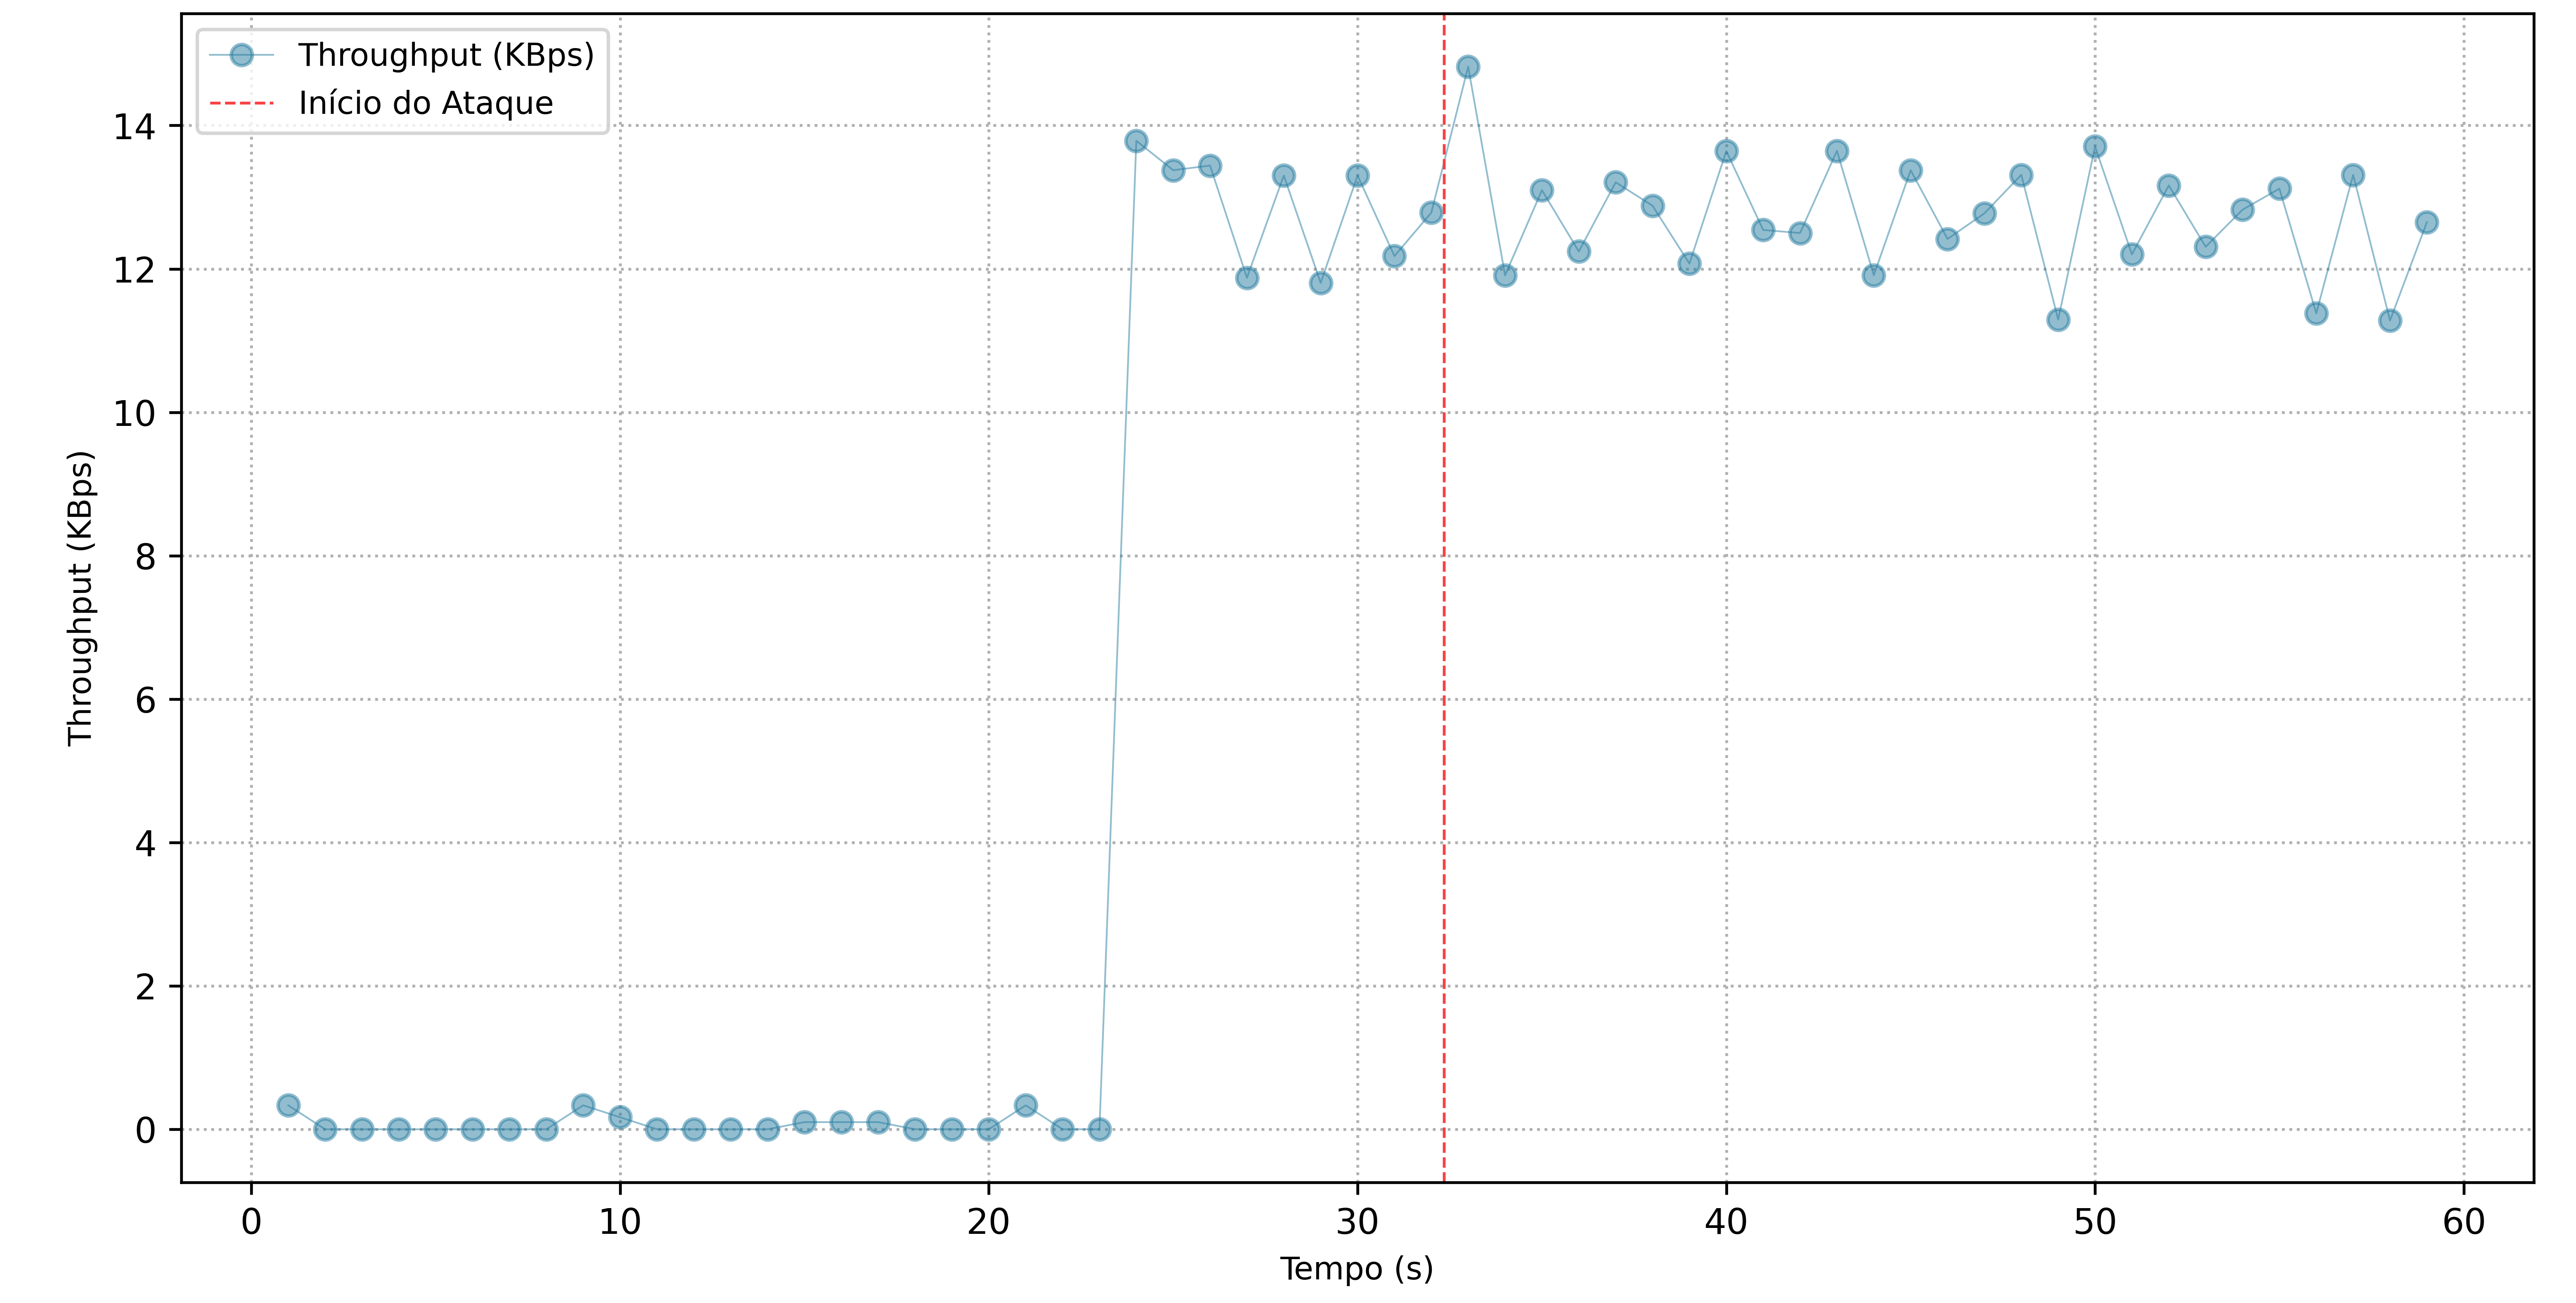
\includegraphics[width=1\textwidth, height=120pt]{USPSC-img/output/cropped/0-dos_certificate_inf_chain_loop-tput.png}
    \end{subfigure}%
    ~ 
    \begin{subfigure}[t]{0.5\textwidth}
        \centering
        \caption{Desempenho}
        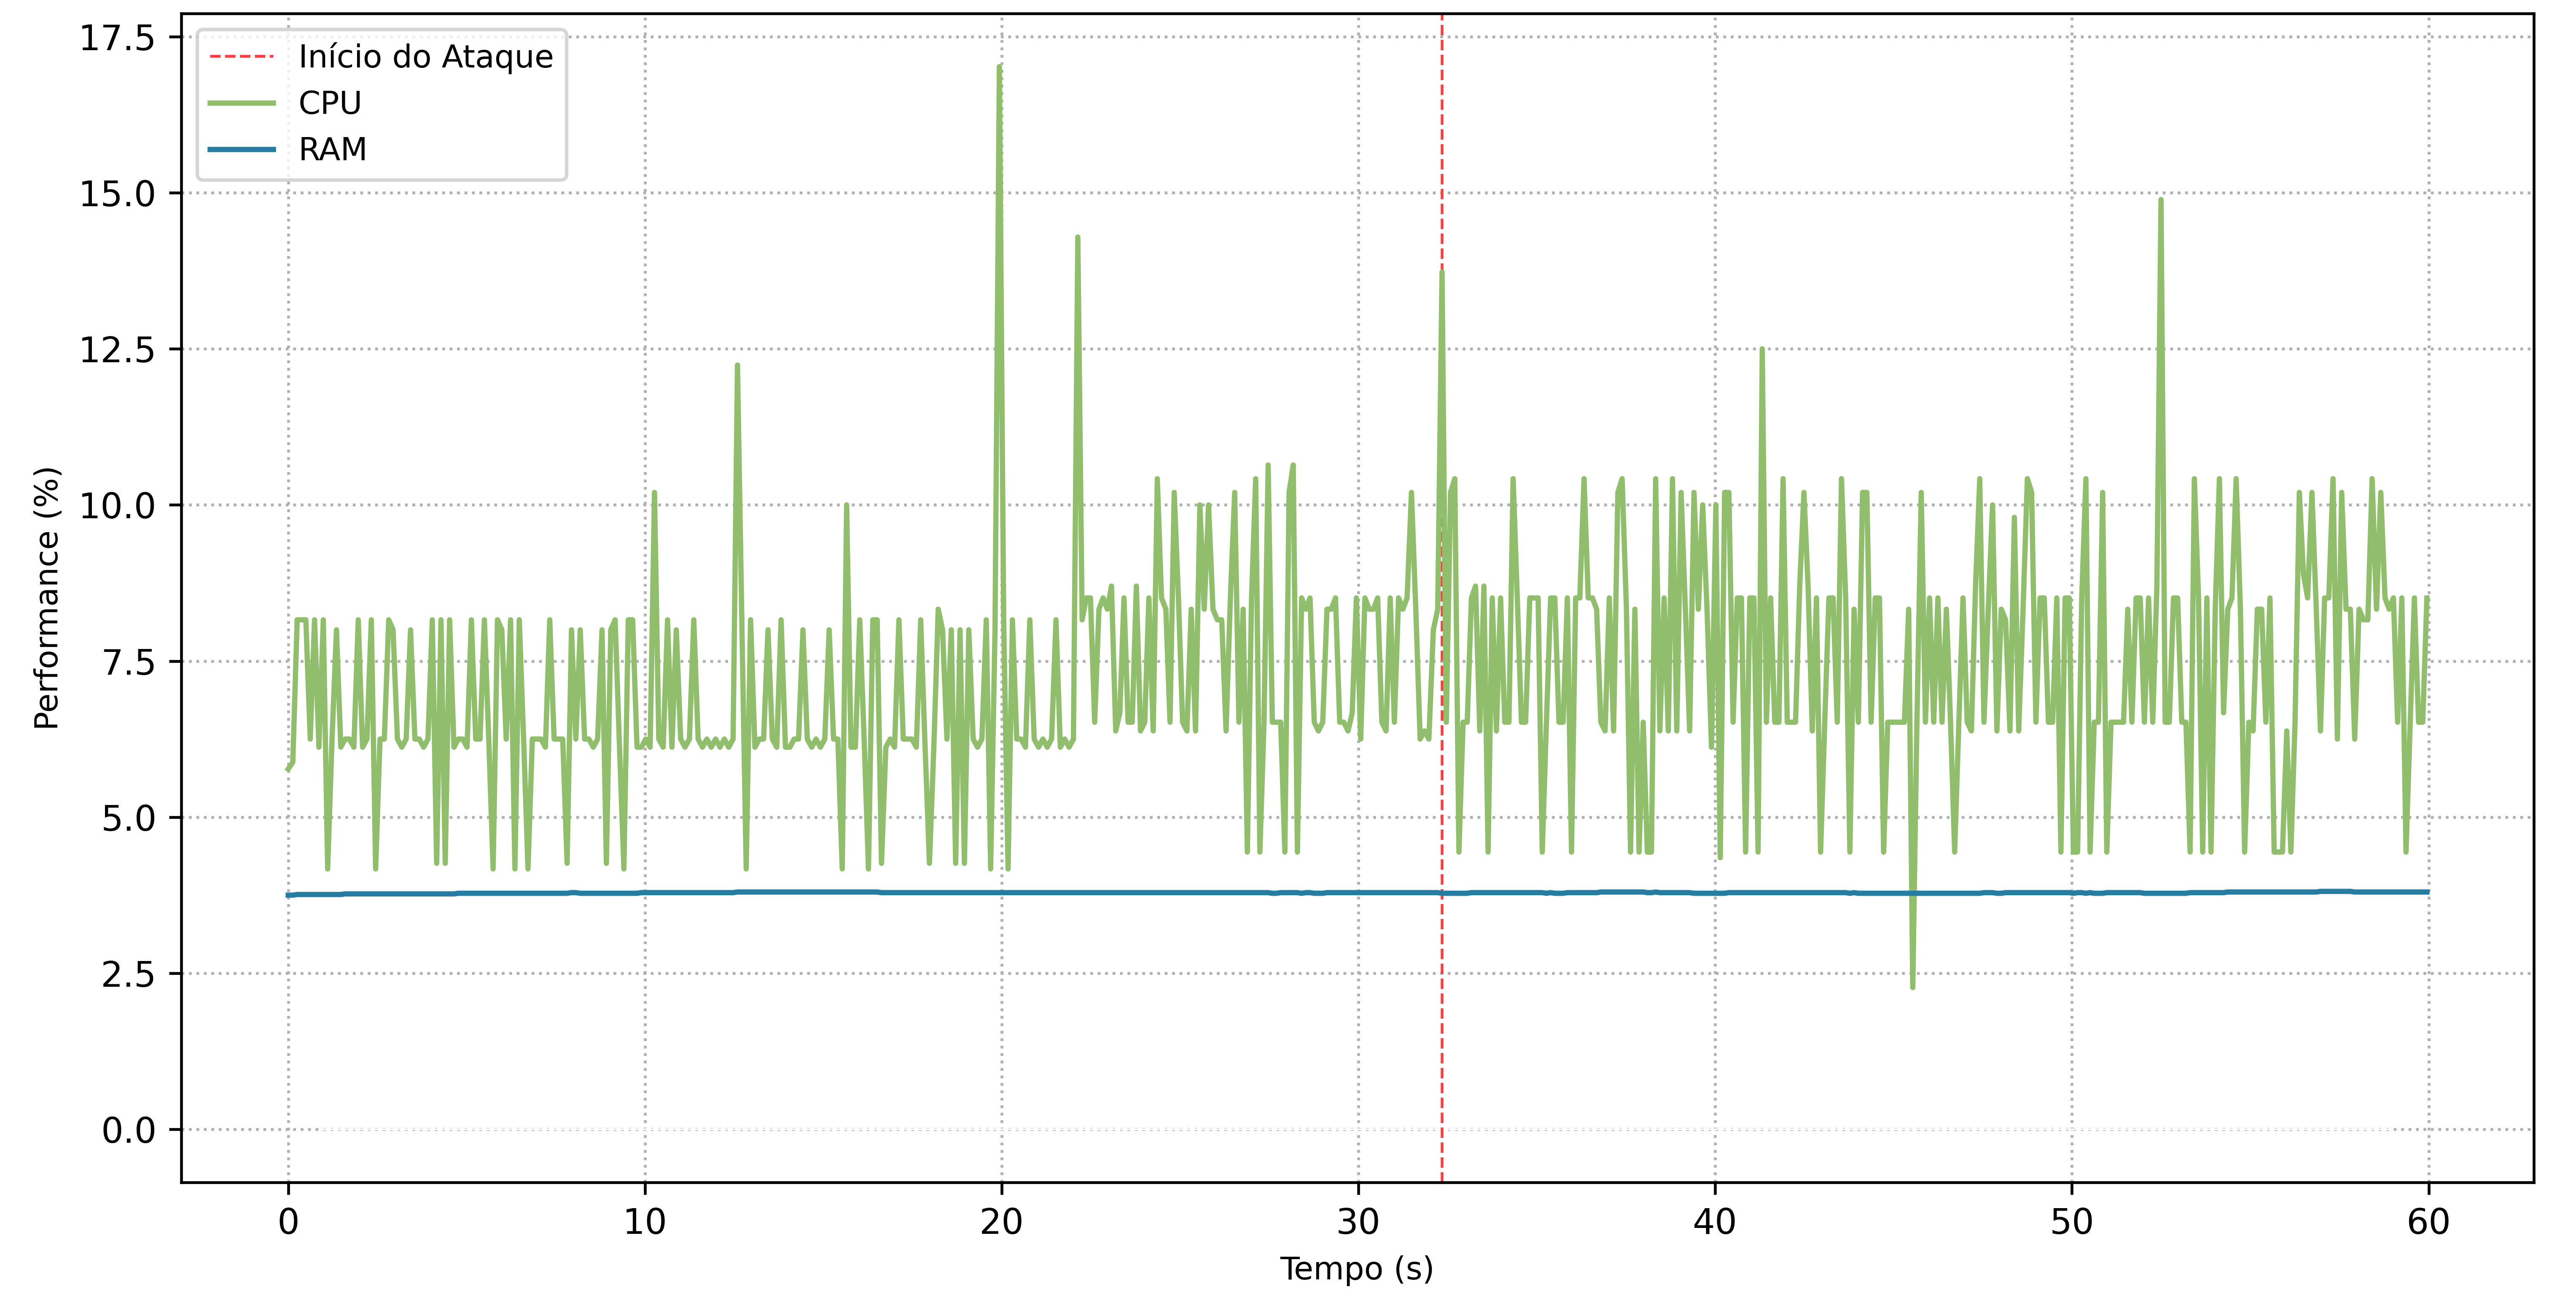
\includegraphics[width=1\textwidth, height=120pt]{USPSC-img/output/cropped/0-dos_certificate_inf_chain_loop-perf.png}
    \end{subfigure}%
    \\
    \begin{subfigure}[t]{0.5\textwidth}
        \centering
        \caption{Pacotes OPC UA}
        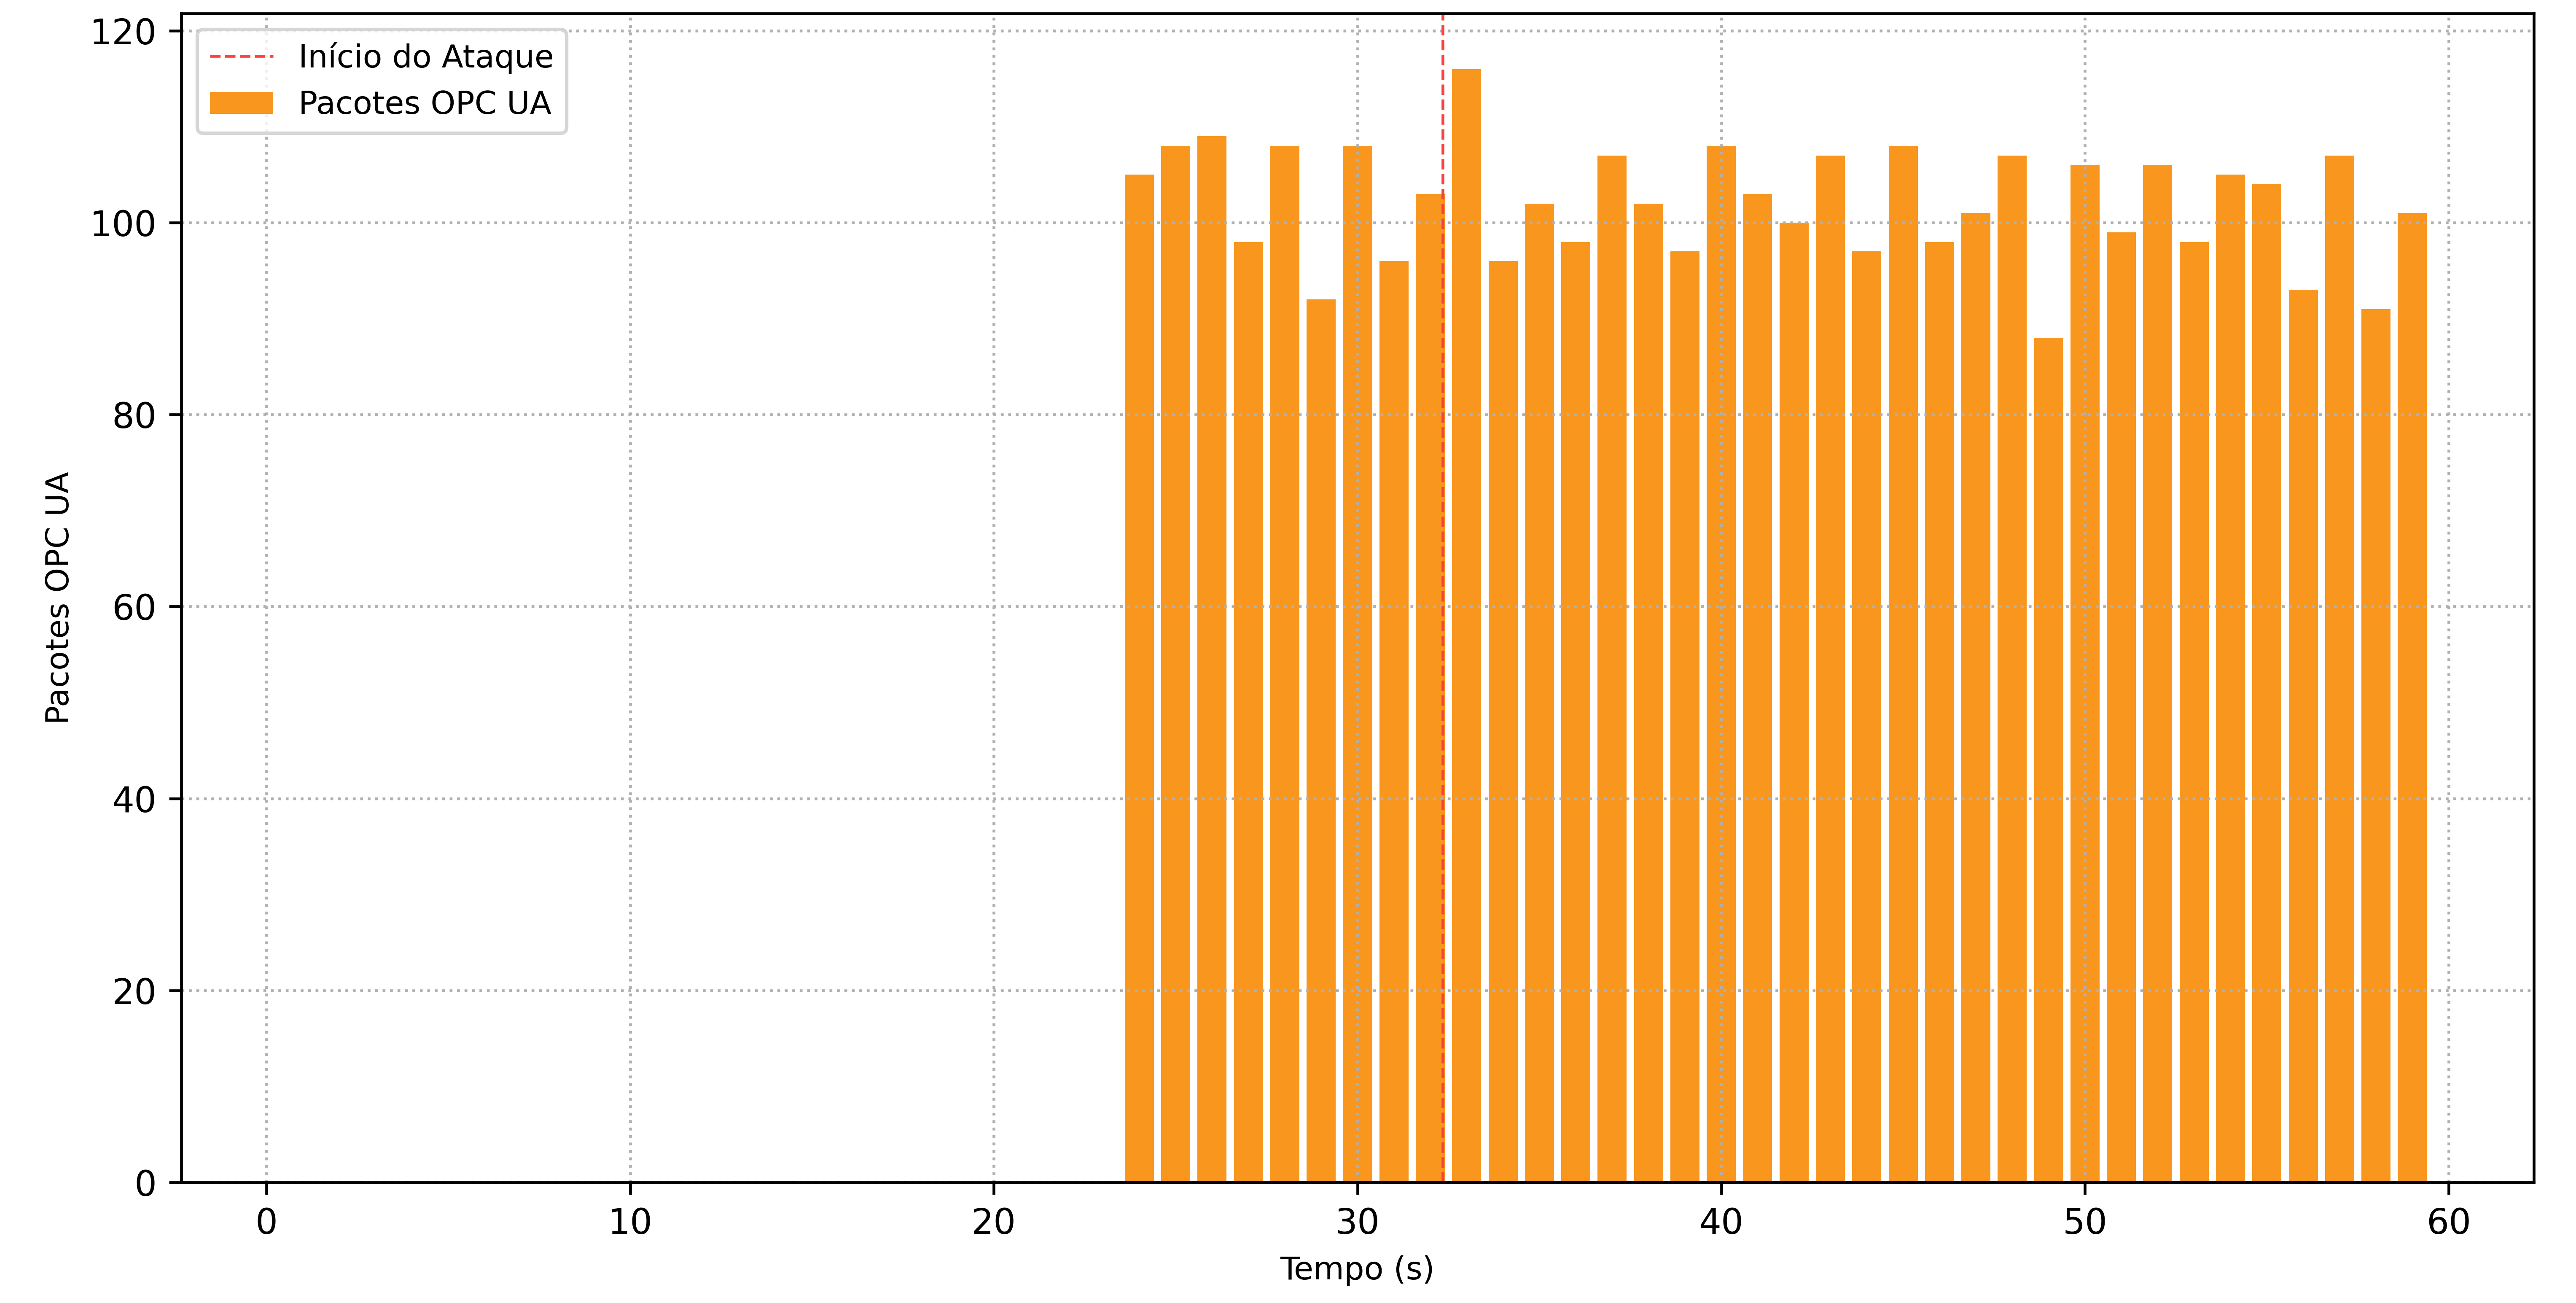
\includegraphics[width=1\textwidth, height=120pt]{USPSC-img/output/cropped/0-dos_certificate_inf_chain_loop-pack.png}
    \end{subfigure}%
    ~
    \begin{subfigure}[t]{0.5\textwidth}
        \centering
        \caption{RTT por pacote}
        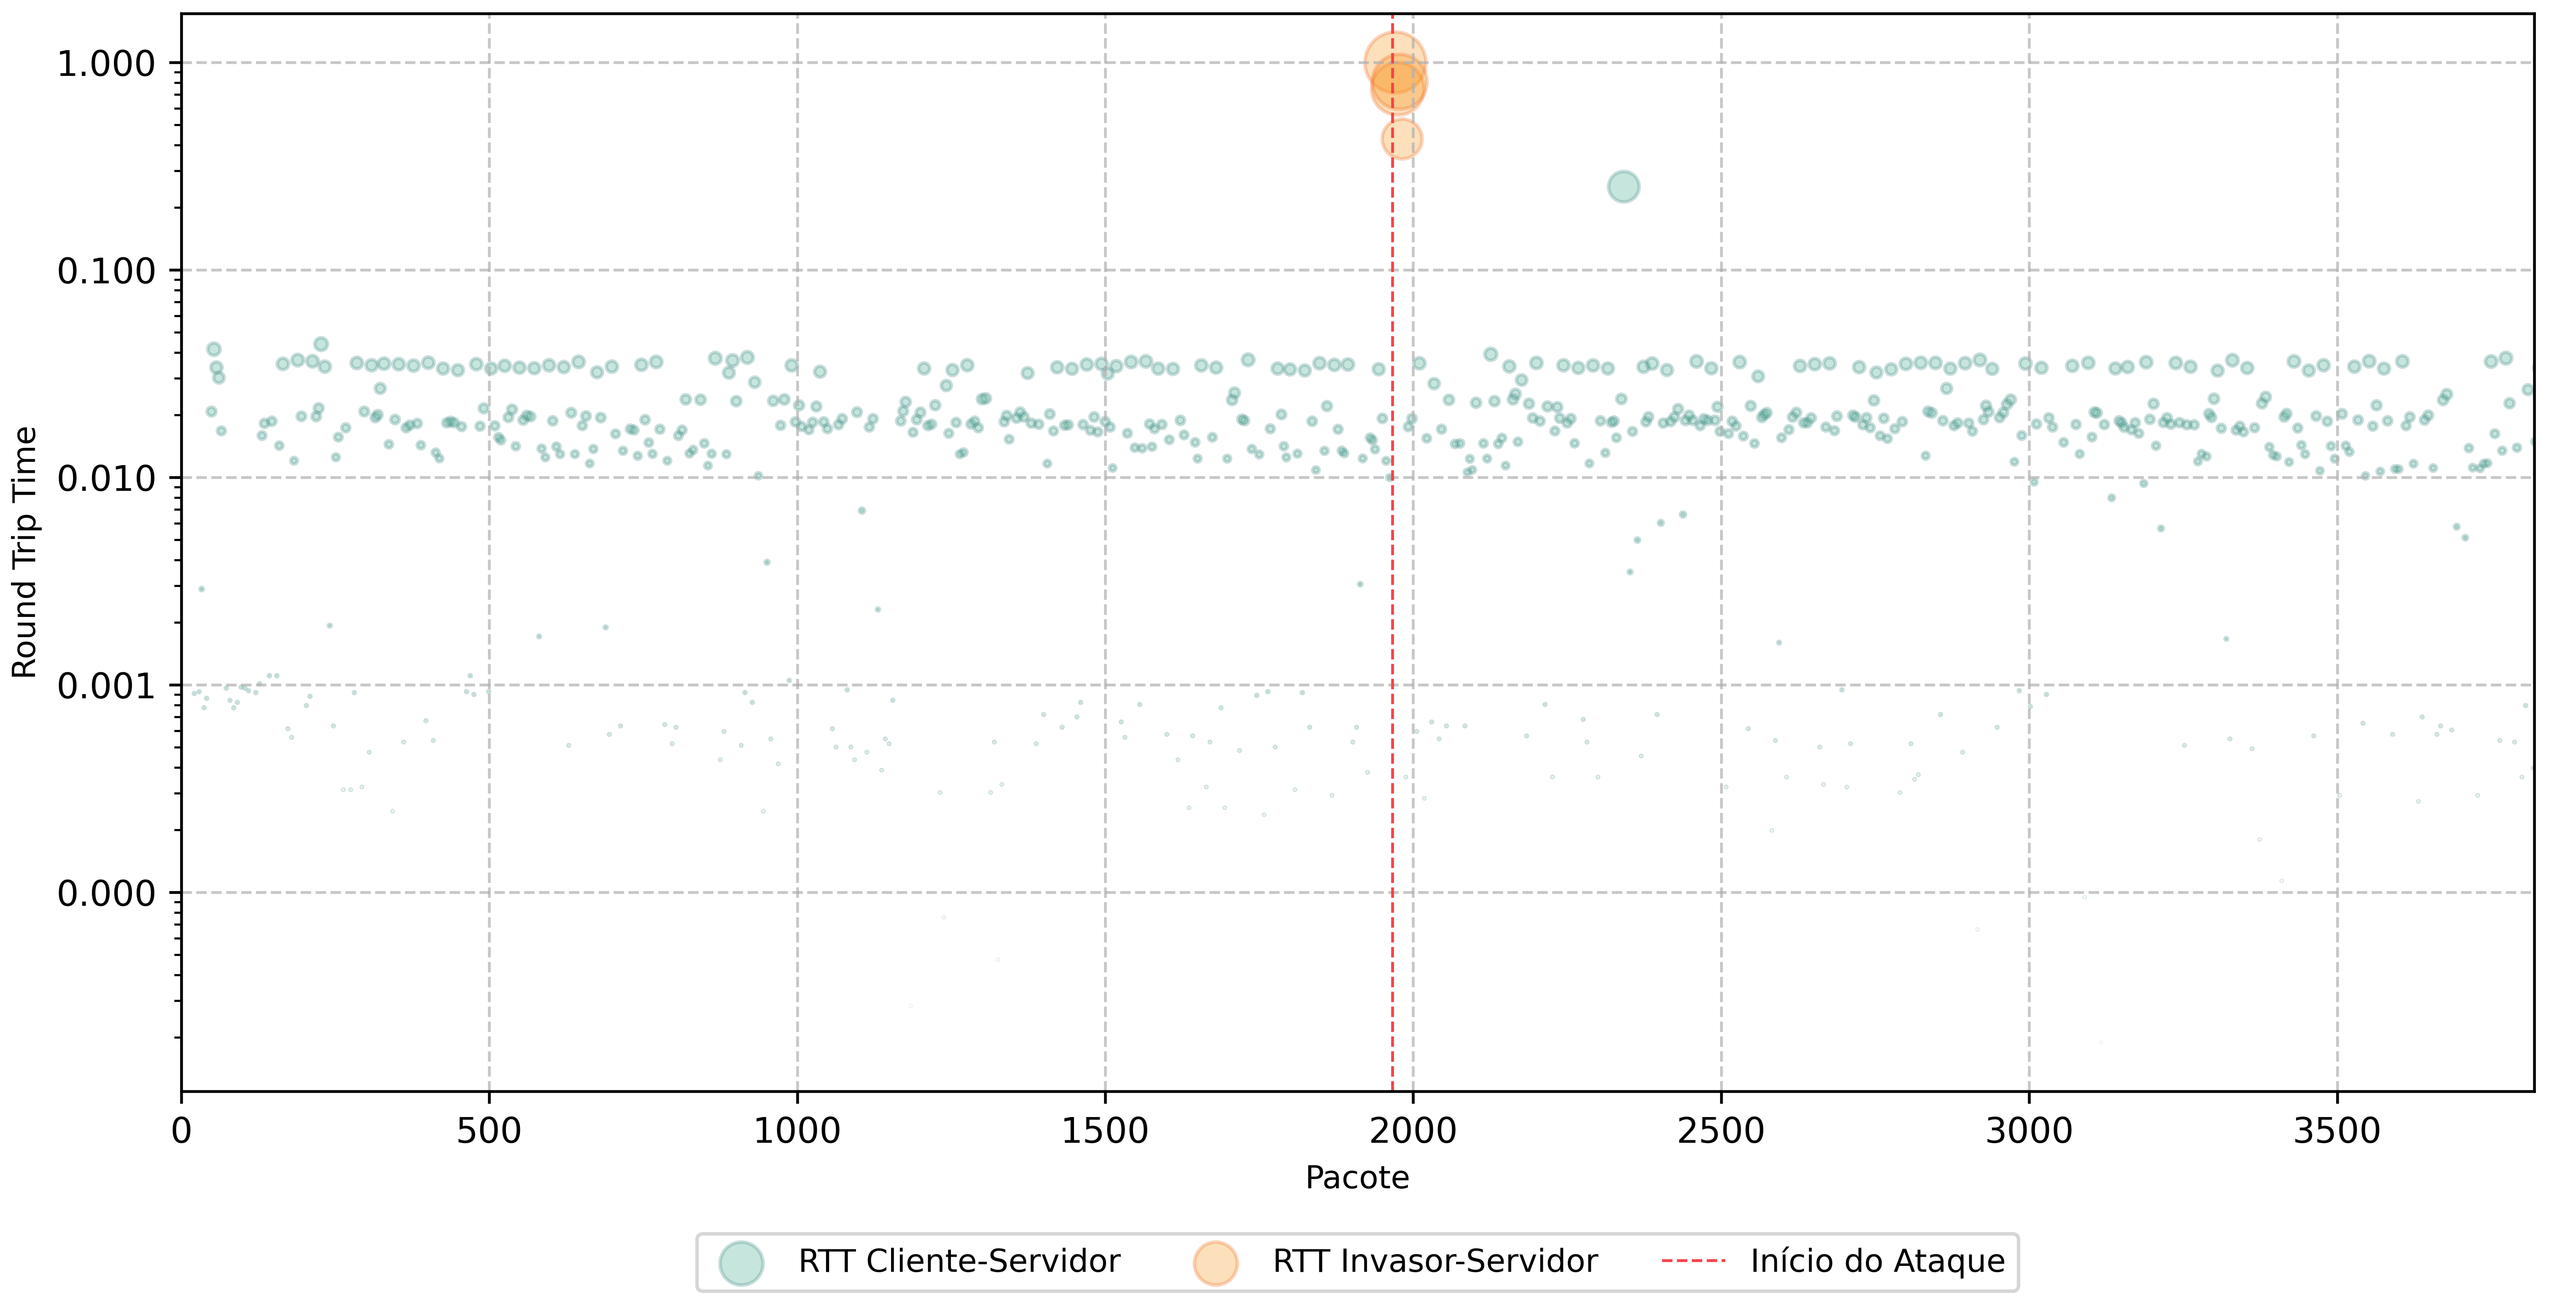
\includegraphics[width=1\textwidth, height=120pt]{USPSC-img/output/cropped/0-dos_certificate_inf_chain_loop-rttp.png}
    \end{subfigure}%
    % ~
    % \begin{subfigure}[t]{0.5\textwidth}
    %     \centering
    %     \caption{RTT por segundos}
    %     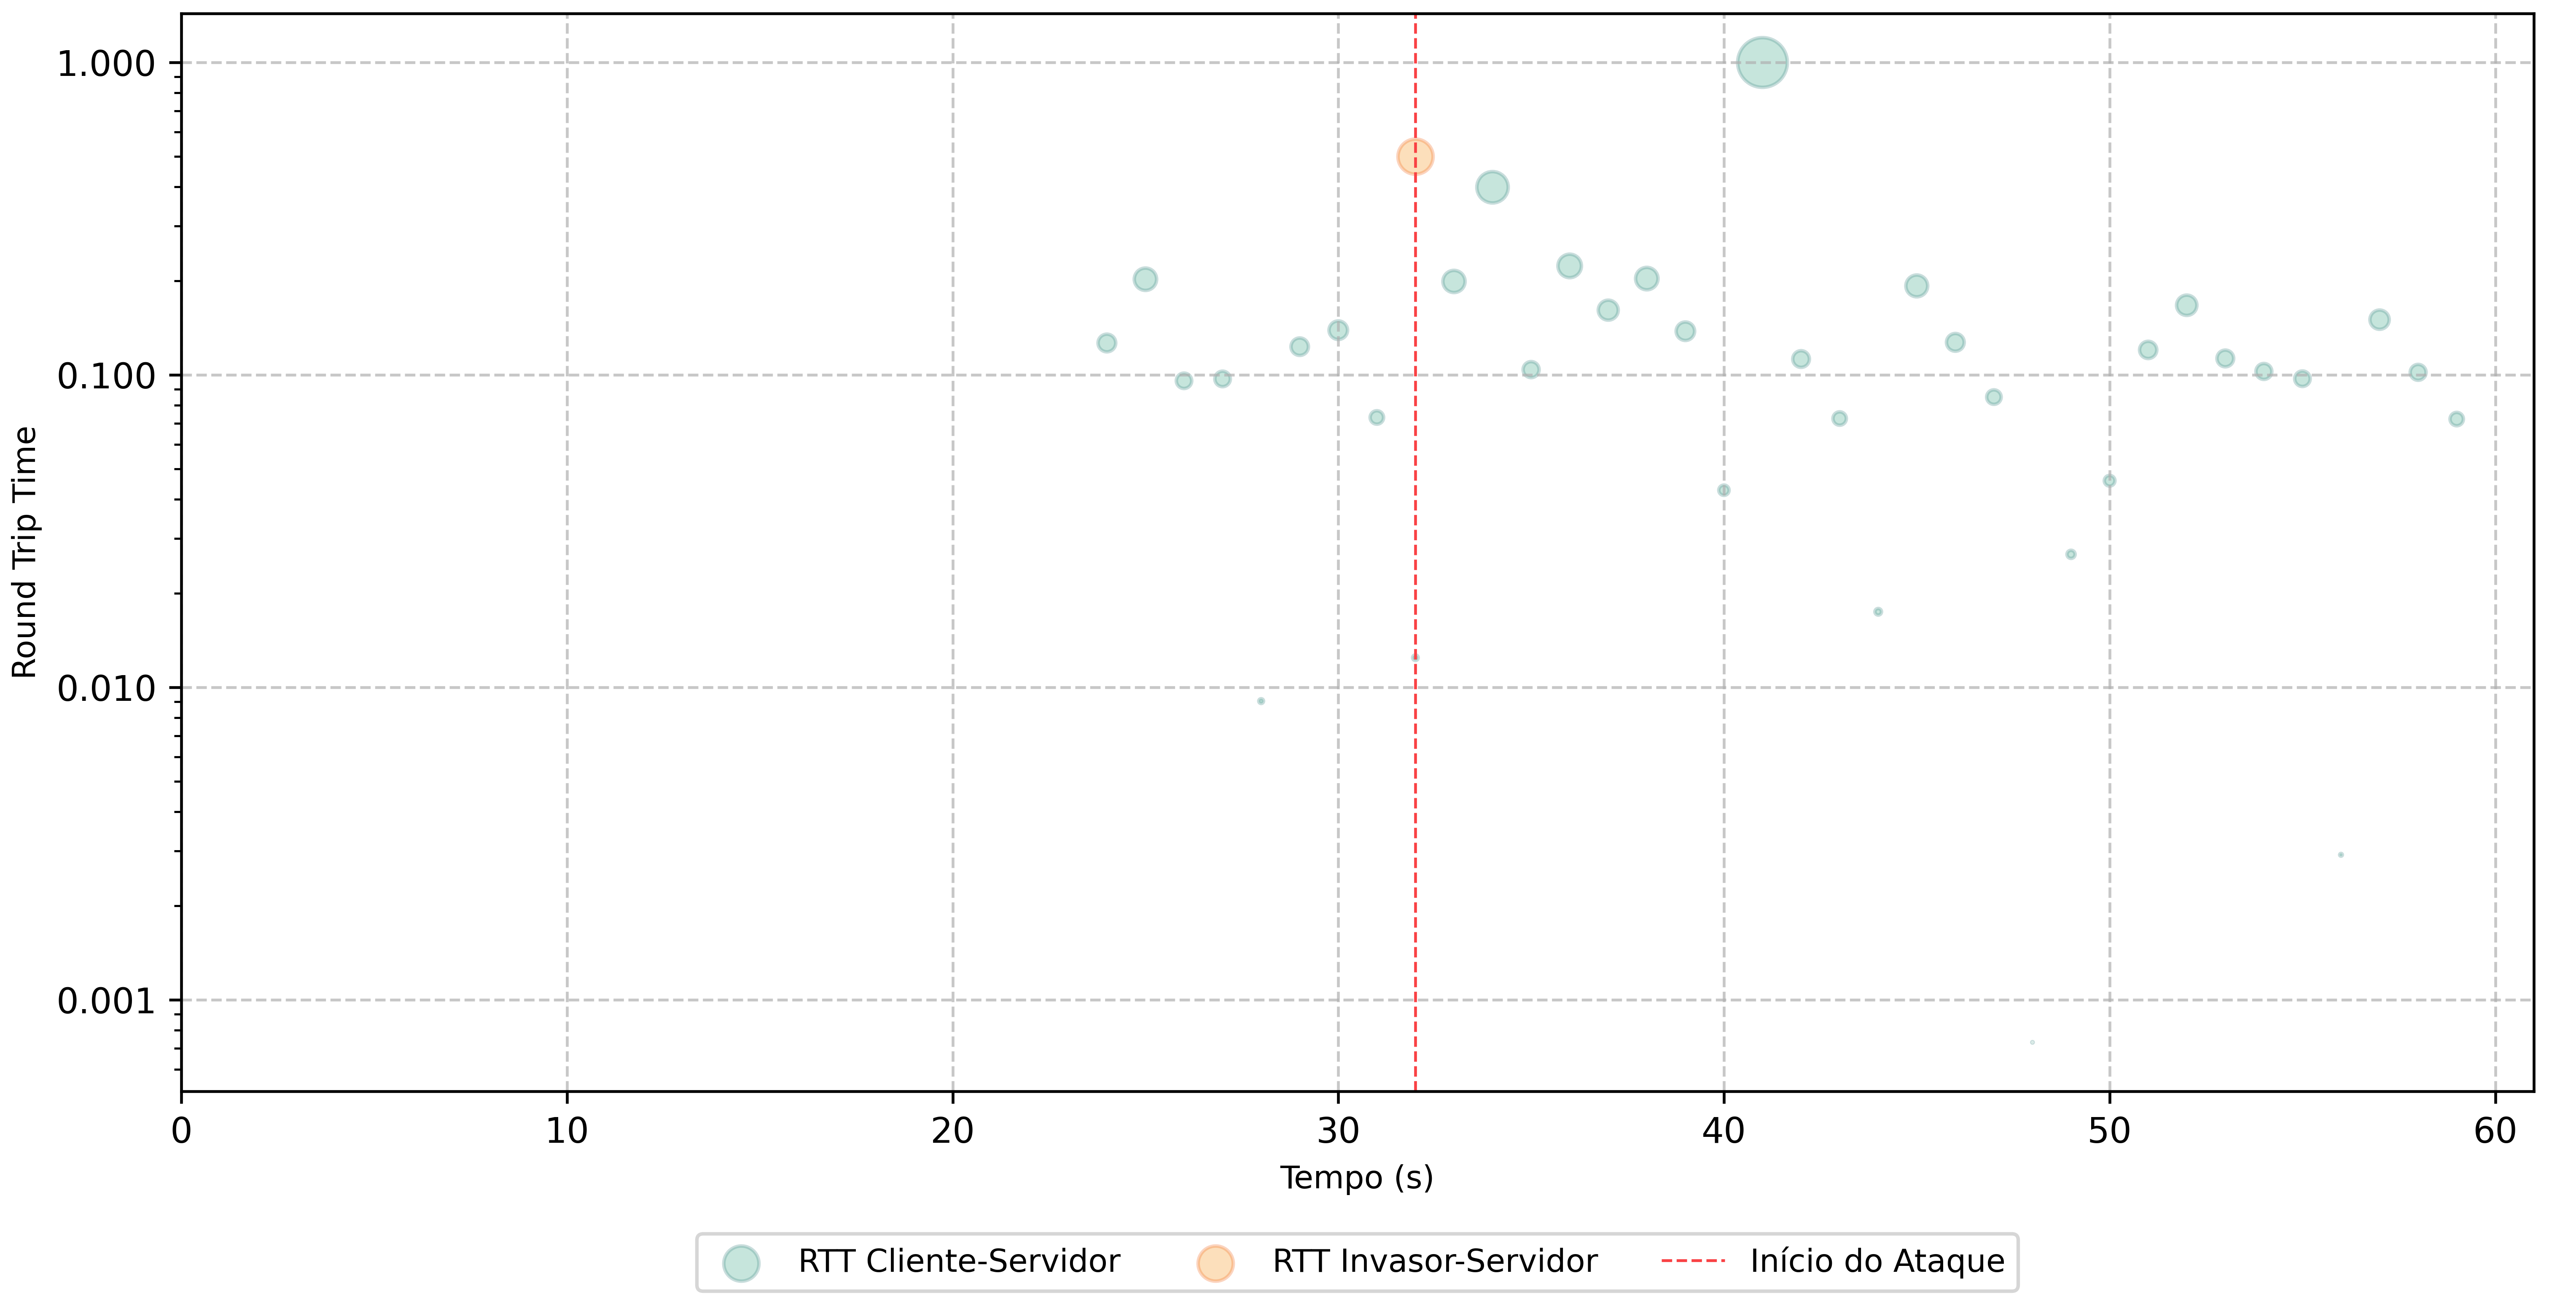
\includegraphics[width=1\textwidth, height=120pt]{USPSC-img/output/cropped/0-dos_certificate_inf_chain_loop-rtts.png}
    % \end{subfigure}%
\end{figure}

\begin{figure}[htbp!]
    \centering
    \caption{\label{fig:1-dos_certificate_inf_chain_loop}Gráficos do ataque de DoS por loop infinito na cadeia de certificados - nível de segurança: `Sign'.}
    \begin{subfigure}[t]{0.5\textwidth}
        \centering
        \caption{\textit{Throughput}}
        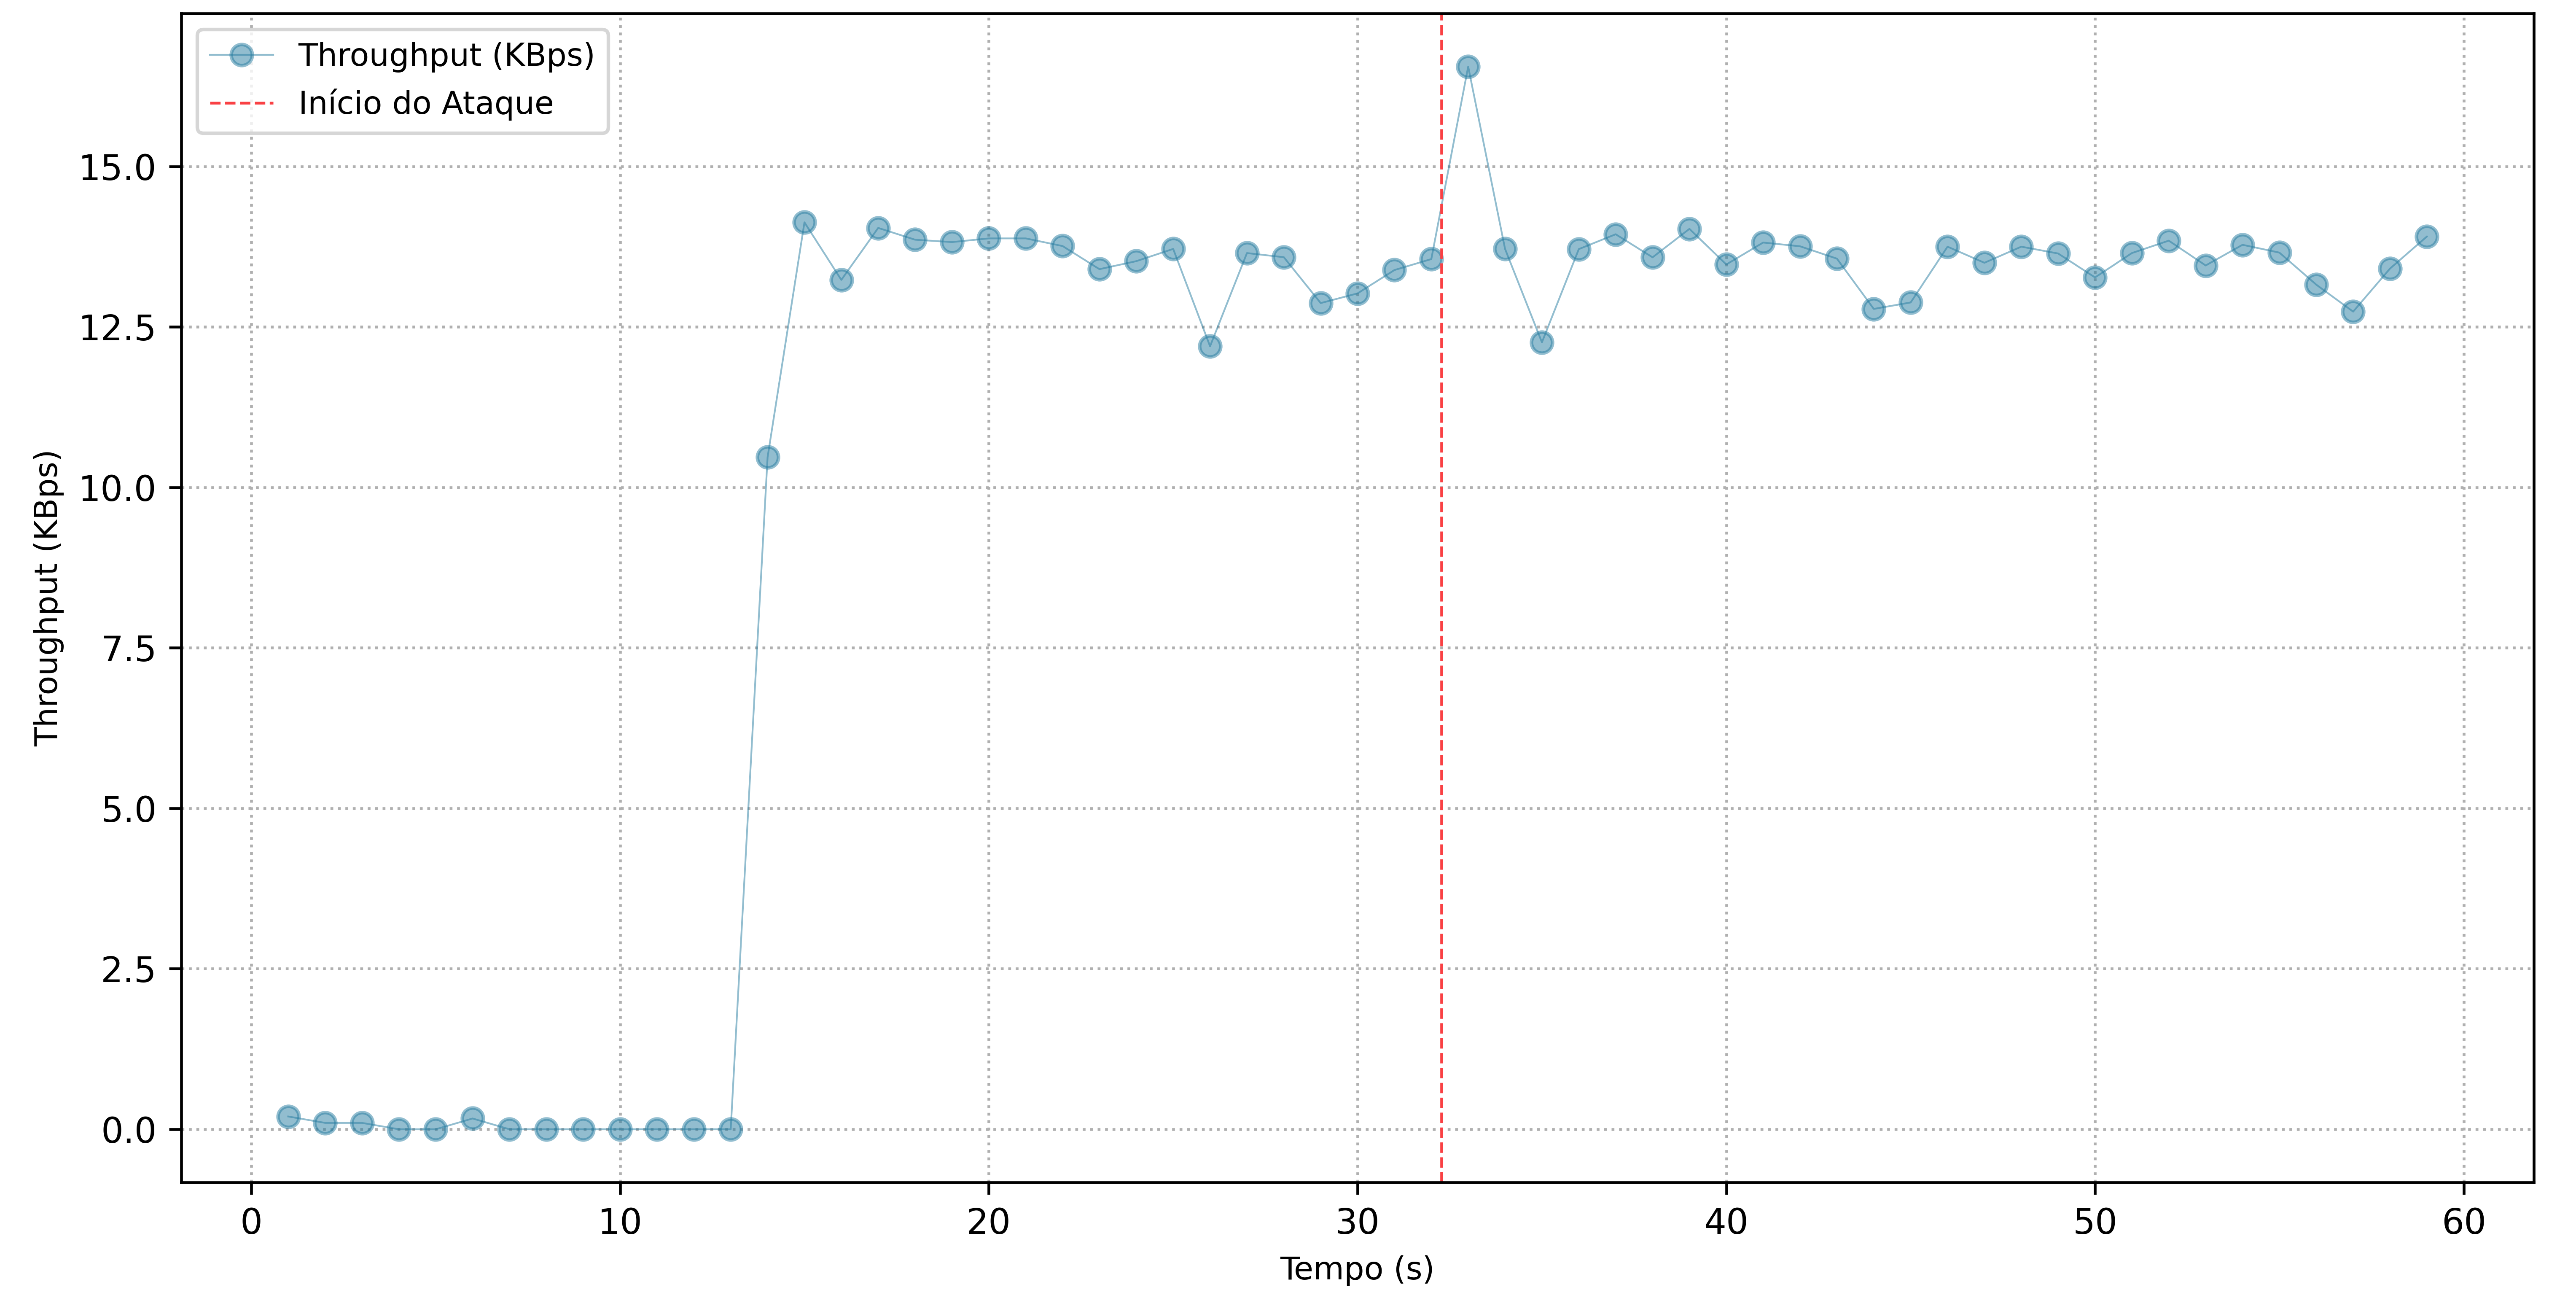
\includegraphics[width=1\textwidth, height=120pt]{USPSC-img/output/cropped/1-dos_certificate_inf_chain_loop-tput.png}
    \end{subfigure}%
    ~ 
    \begin{subfigure}[t]{0.5\textwidth}
        \centering
        \caption{Desempenho}
        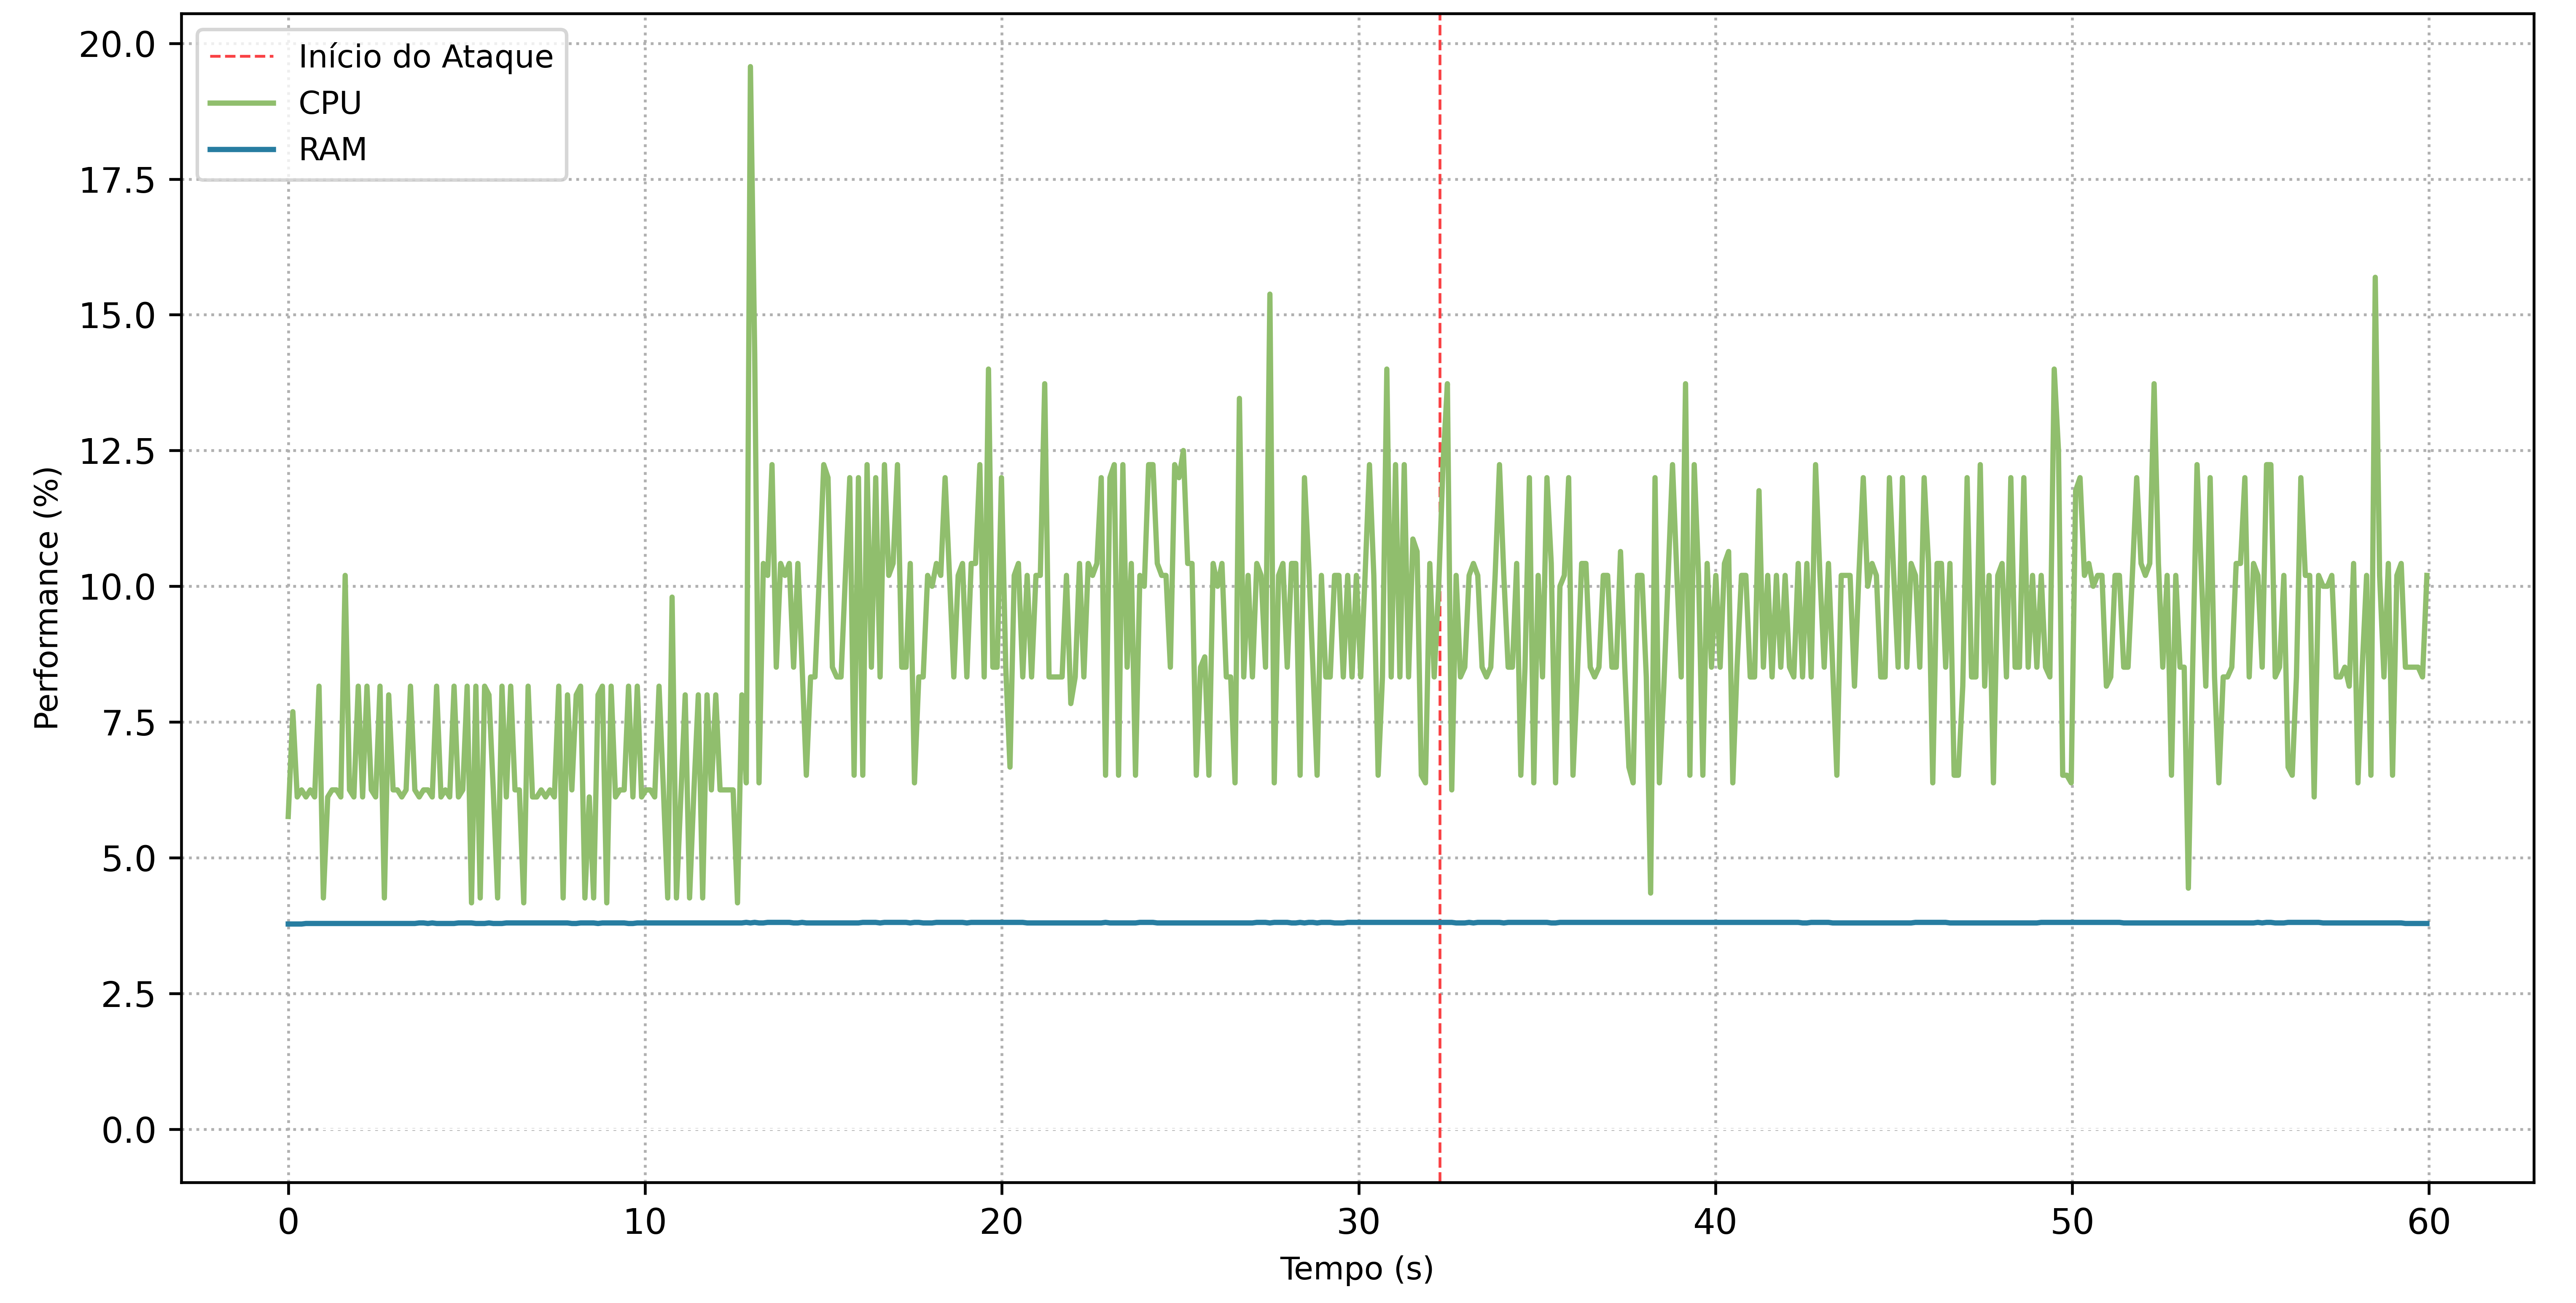
\includegraphics[width=1\textwidth, height=120pt]{USPSC-img/output/cropped/1-dos_certificate_inf_chain_loop-perf.png}
    \end{subfigure}%
    \\
    \begin{subfigure}[t]{0.5\textwidth}
        \centering
        \caption{Pacotes OPC UA}
        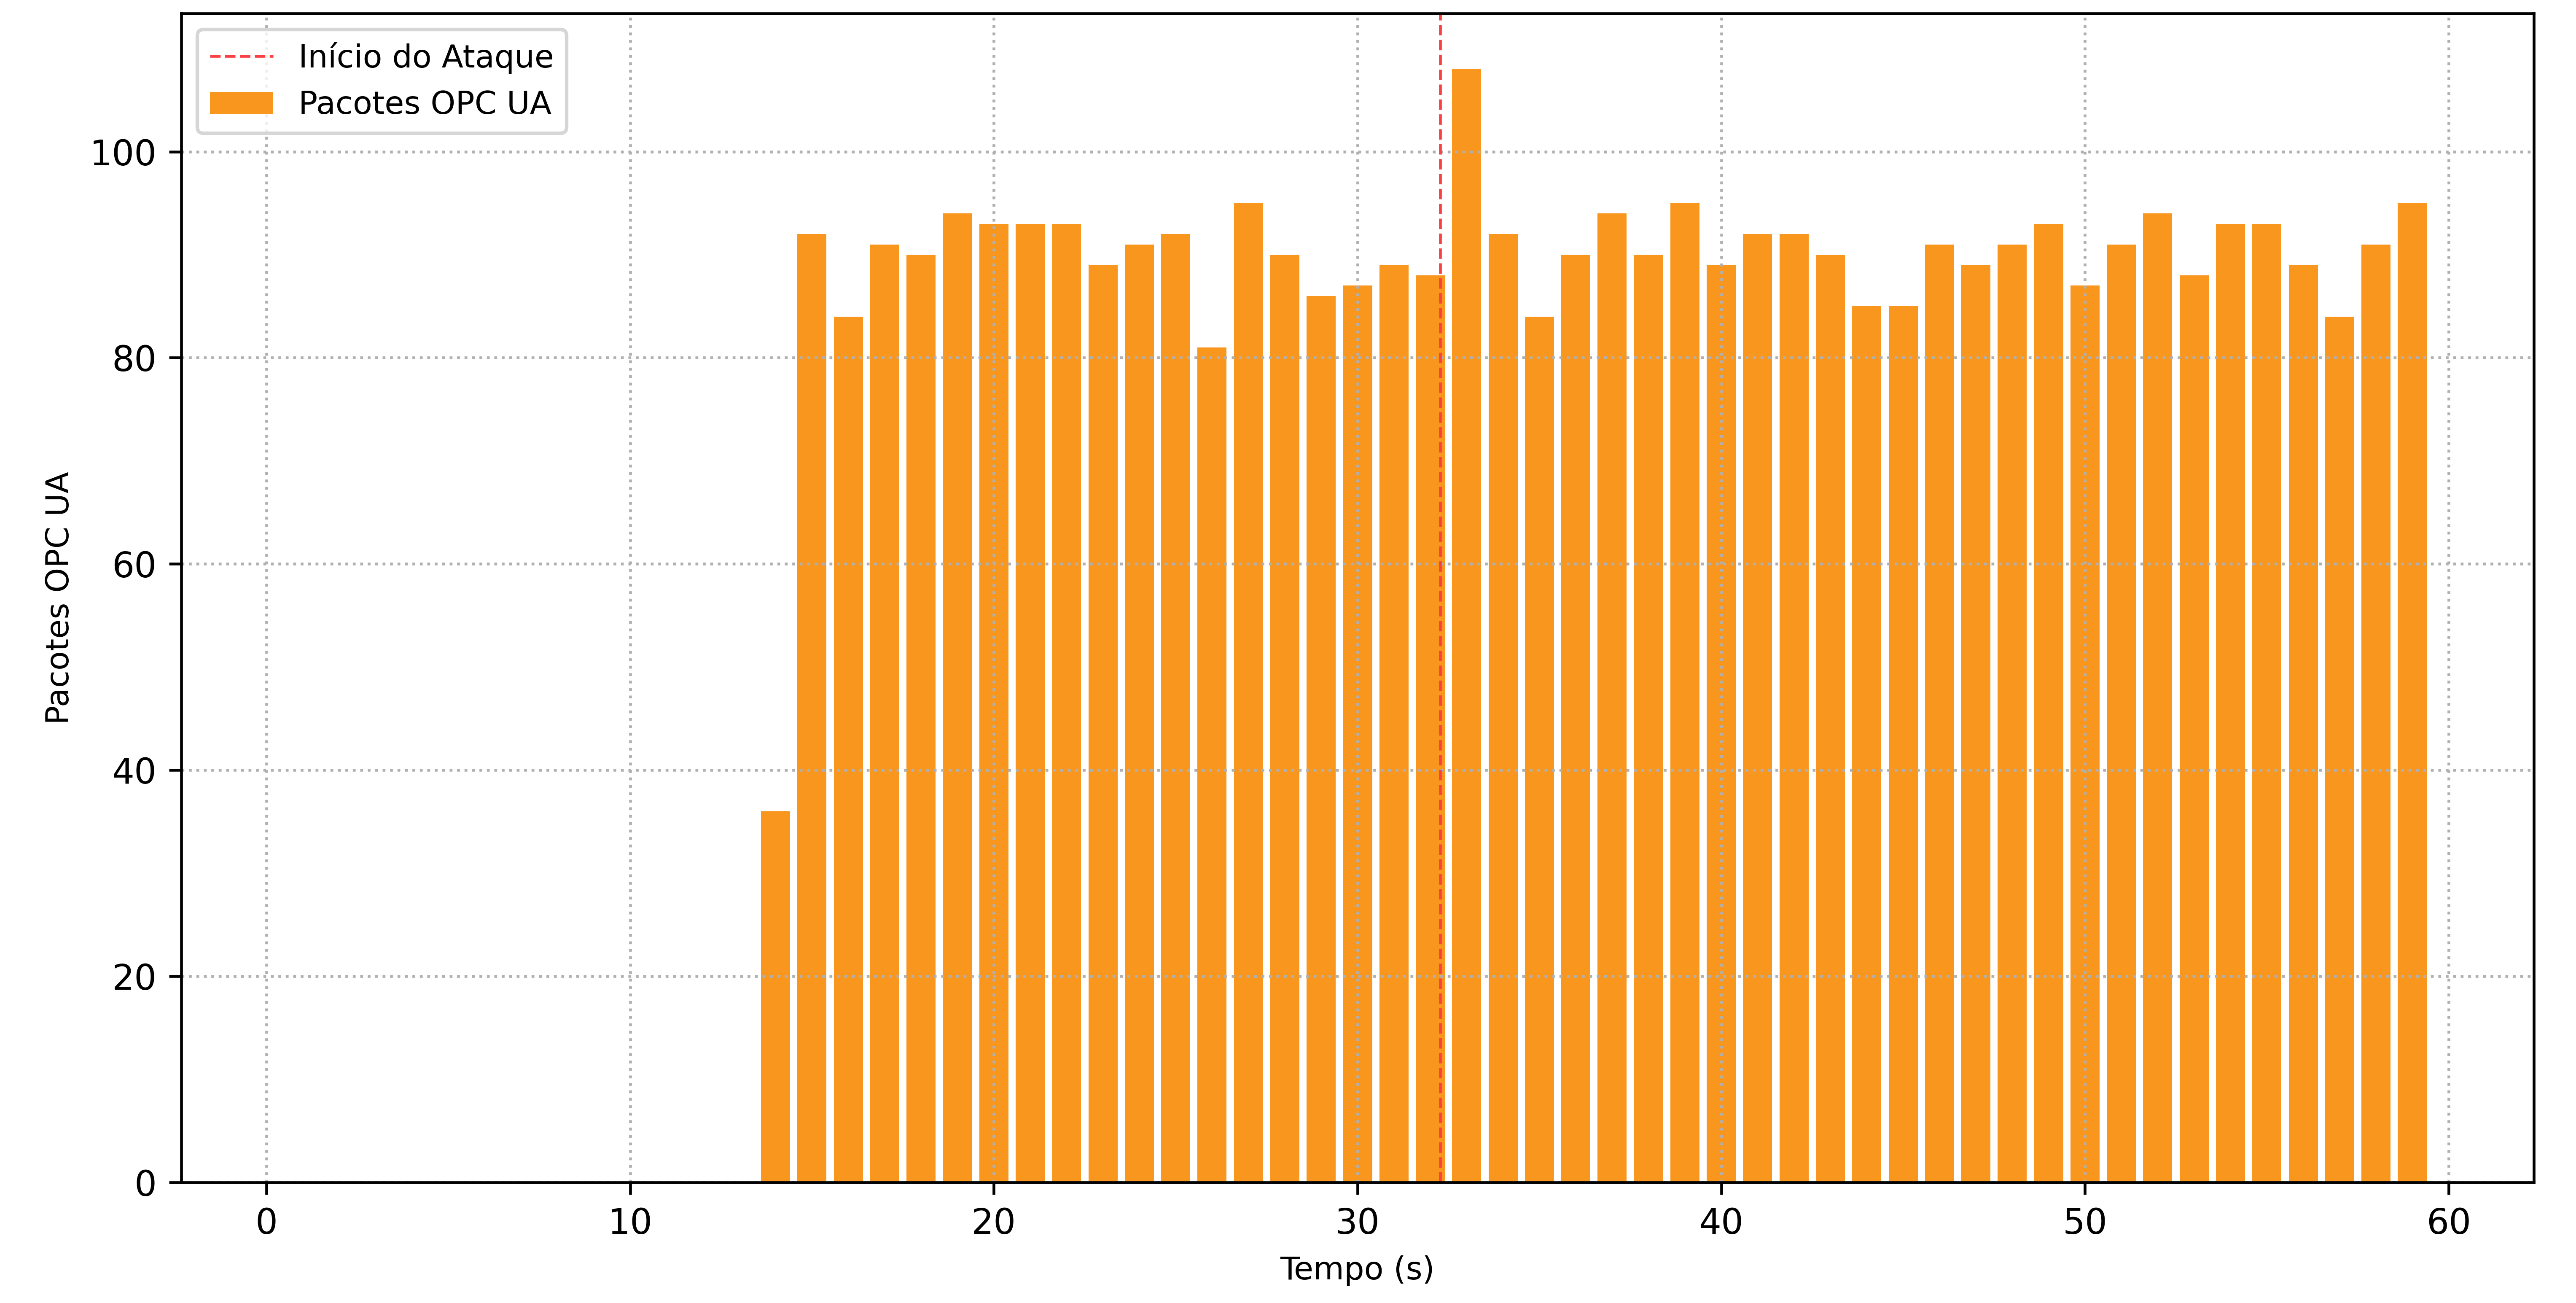
\includegraphics[width=1\textwidth, height=120pt]{USPSC-img/output/cropped/1-dos_certificate_inf_chain_loop-pack.png}
    \end{subfigure}%
    ~
    \begin{subfigure}[t]{0.5\textwidth}
        \centering
        \caption{RTT por pacote}
        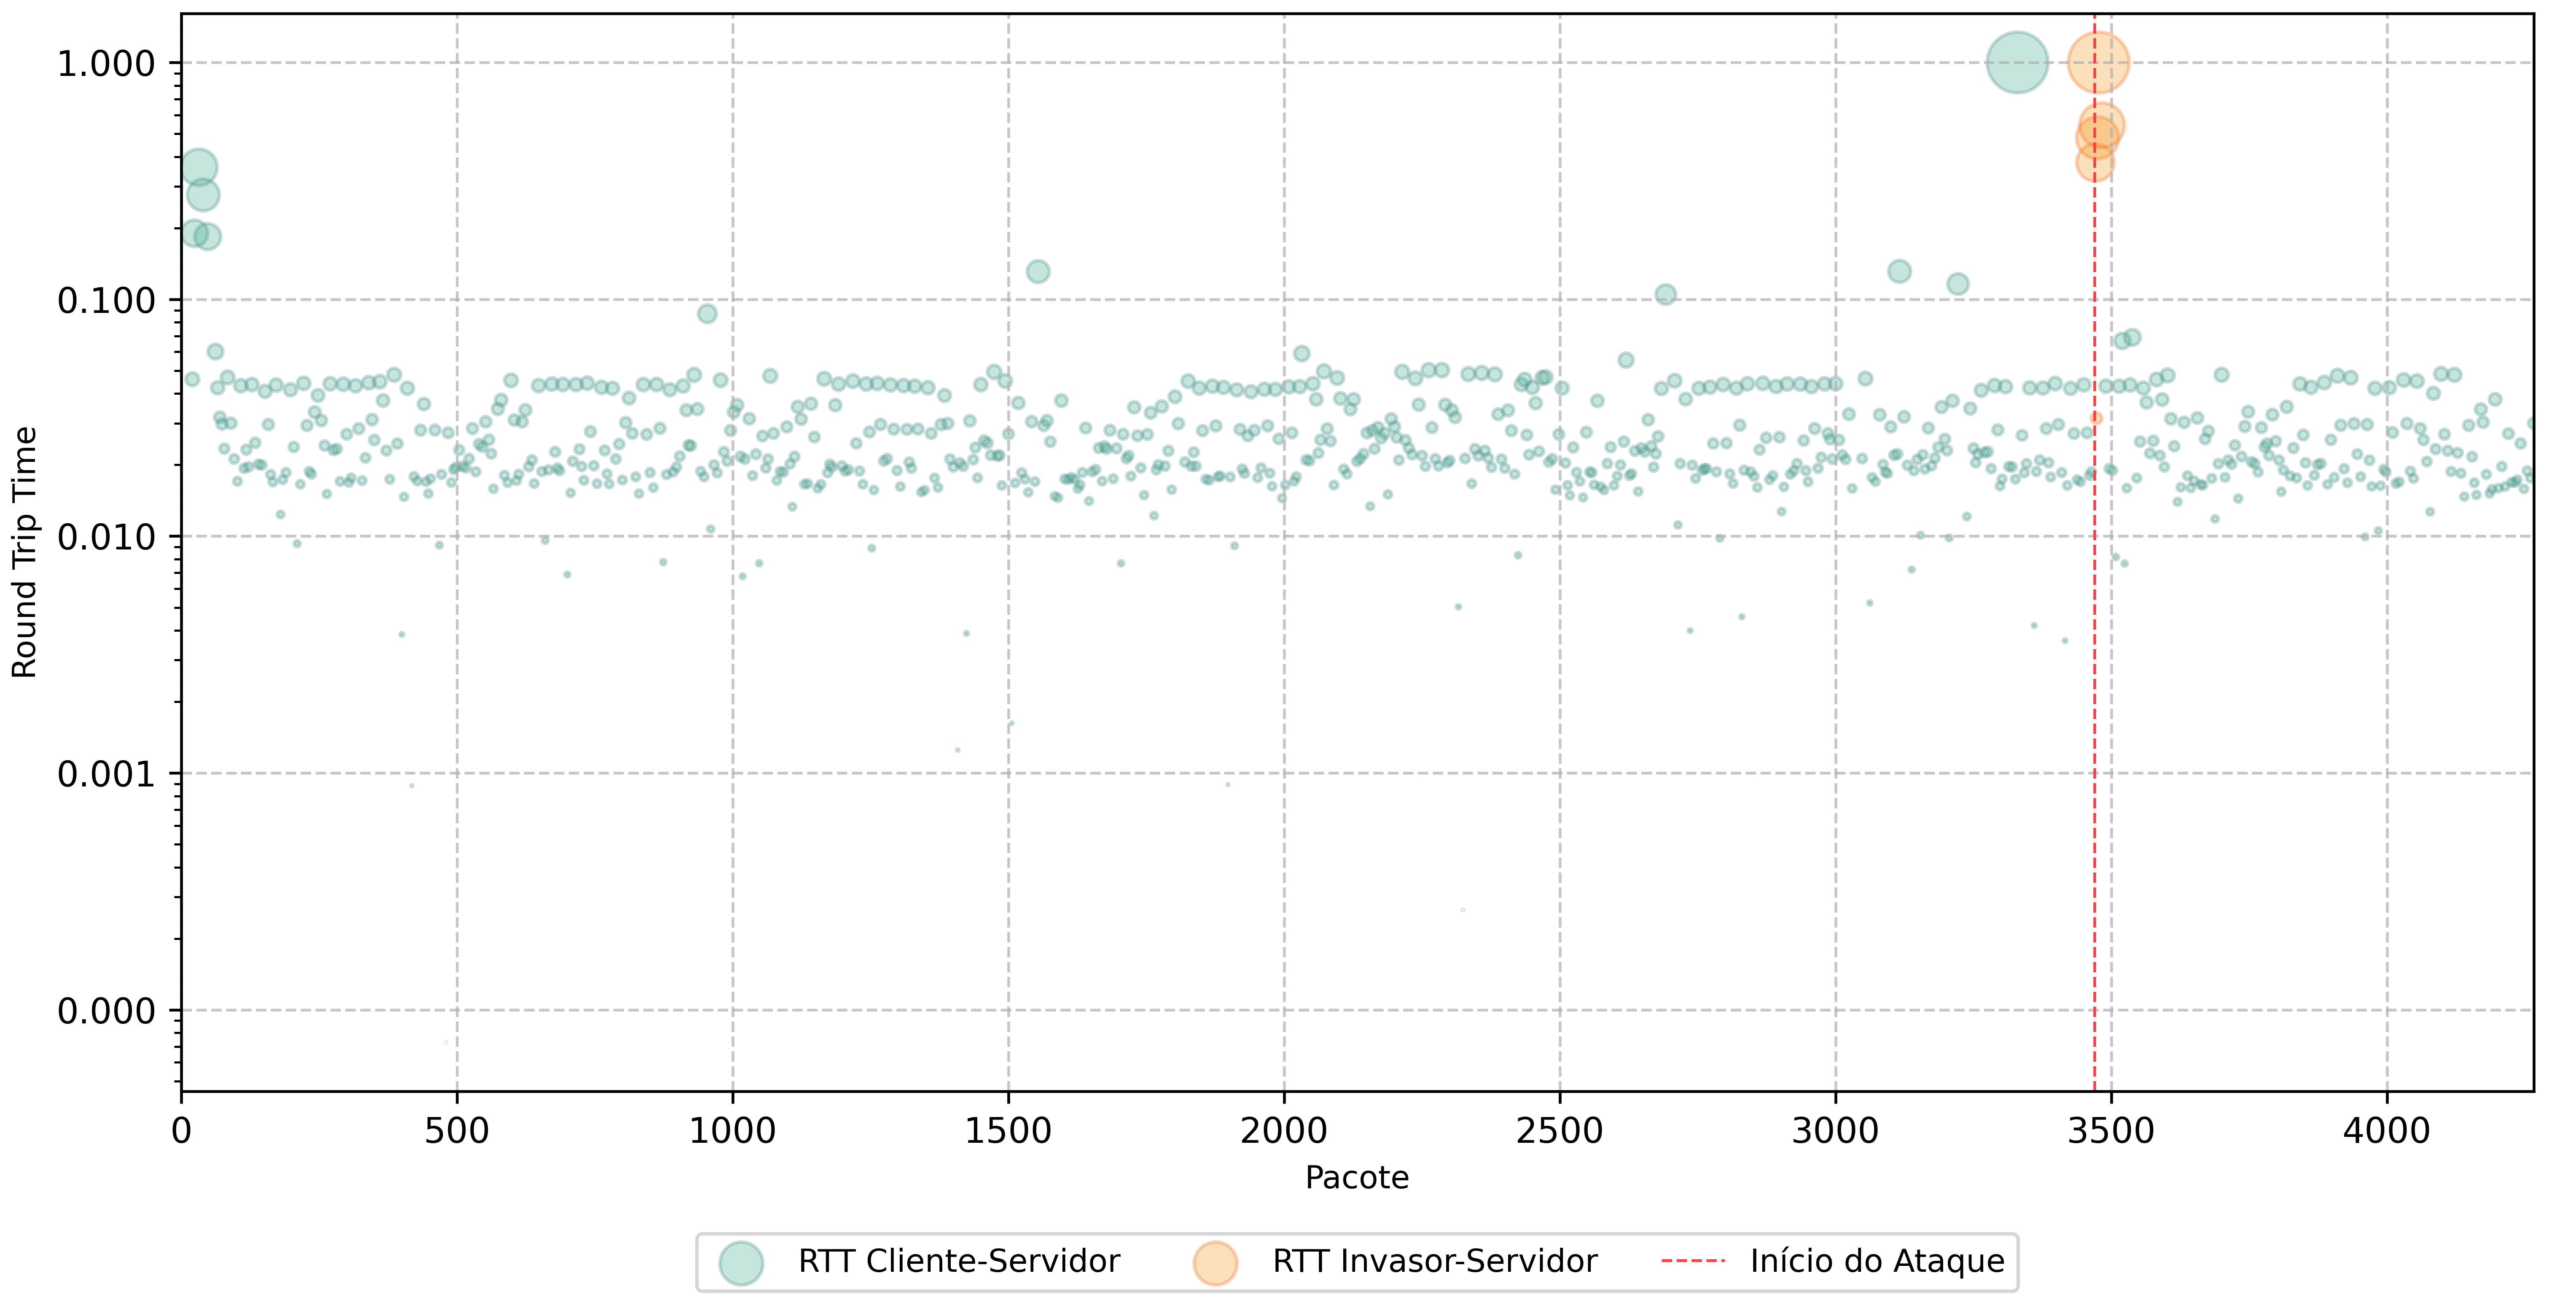
\includegraphics[width=1\textwidth, height=120pt]{USPSC-img/output/cropped/1-dos_certificate_inf_chain_loop-rttp.png}
    \end{subfigure}%
    % ~
    % \begin{subfigure}[t]{0.5\textwidth}
    %     \centering
    %     \caption{RTT por segundos}
    %     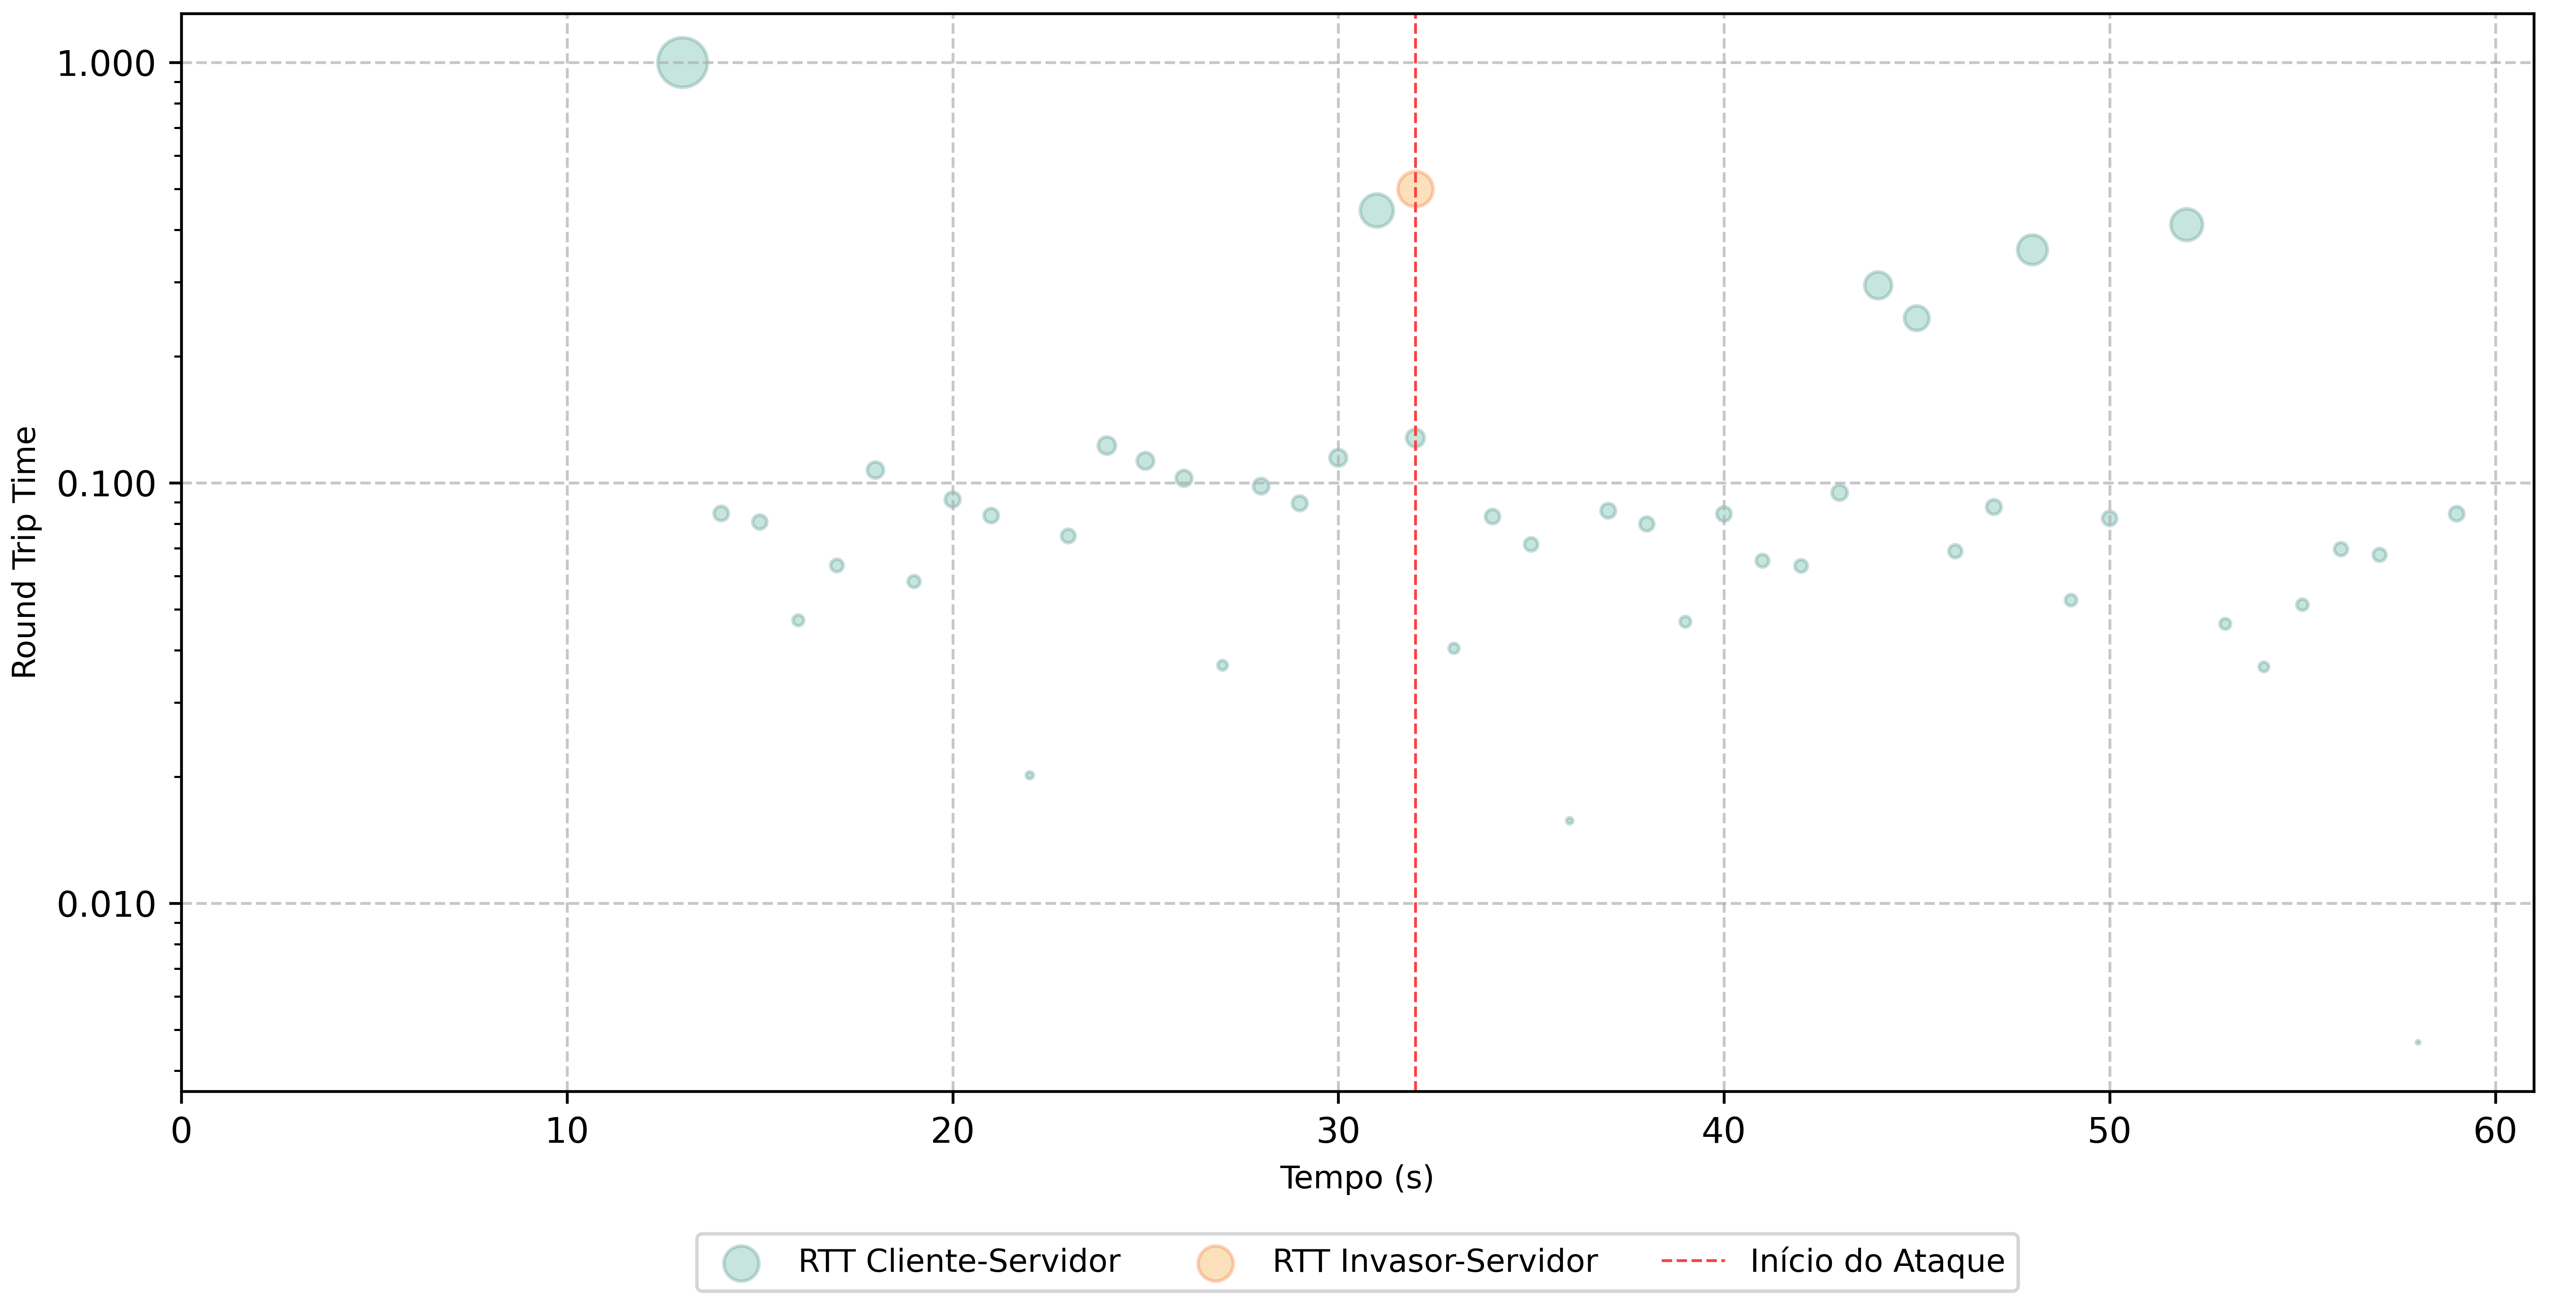
\includegraphics[width=1\textwidth, height=120pt]{USPSC-img/output/cropped/1-dos_certificate_inf_chain_loop-rtts.png}
    % \end{subfigure}%
\end{figure}

\begin{figure}[htbp!]
    \centering
    \caption{\label{fig:2-dos_certificate_inf_chain_loop}Gráficos do ataque de DoS por loop infinito na cadeia de certificados - nível de segurança: `Sign \& Encrypt'.}
    \begin{subfigure}[t]{0.5\textwidth}
        \centering
        \caption{\textit{Throughput}}
        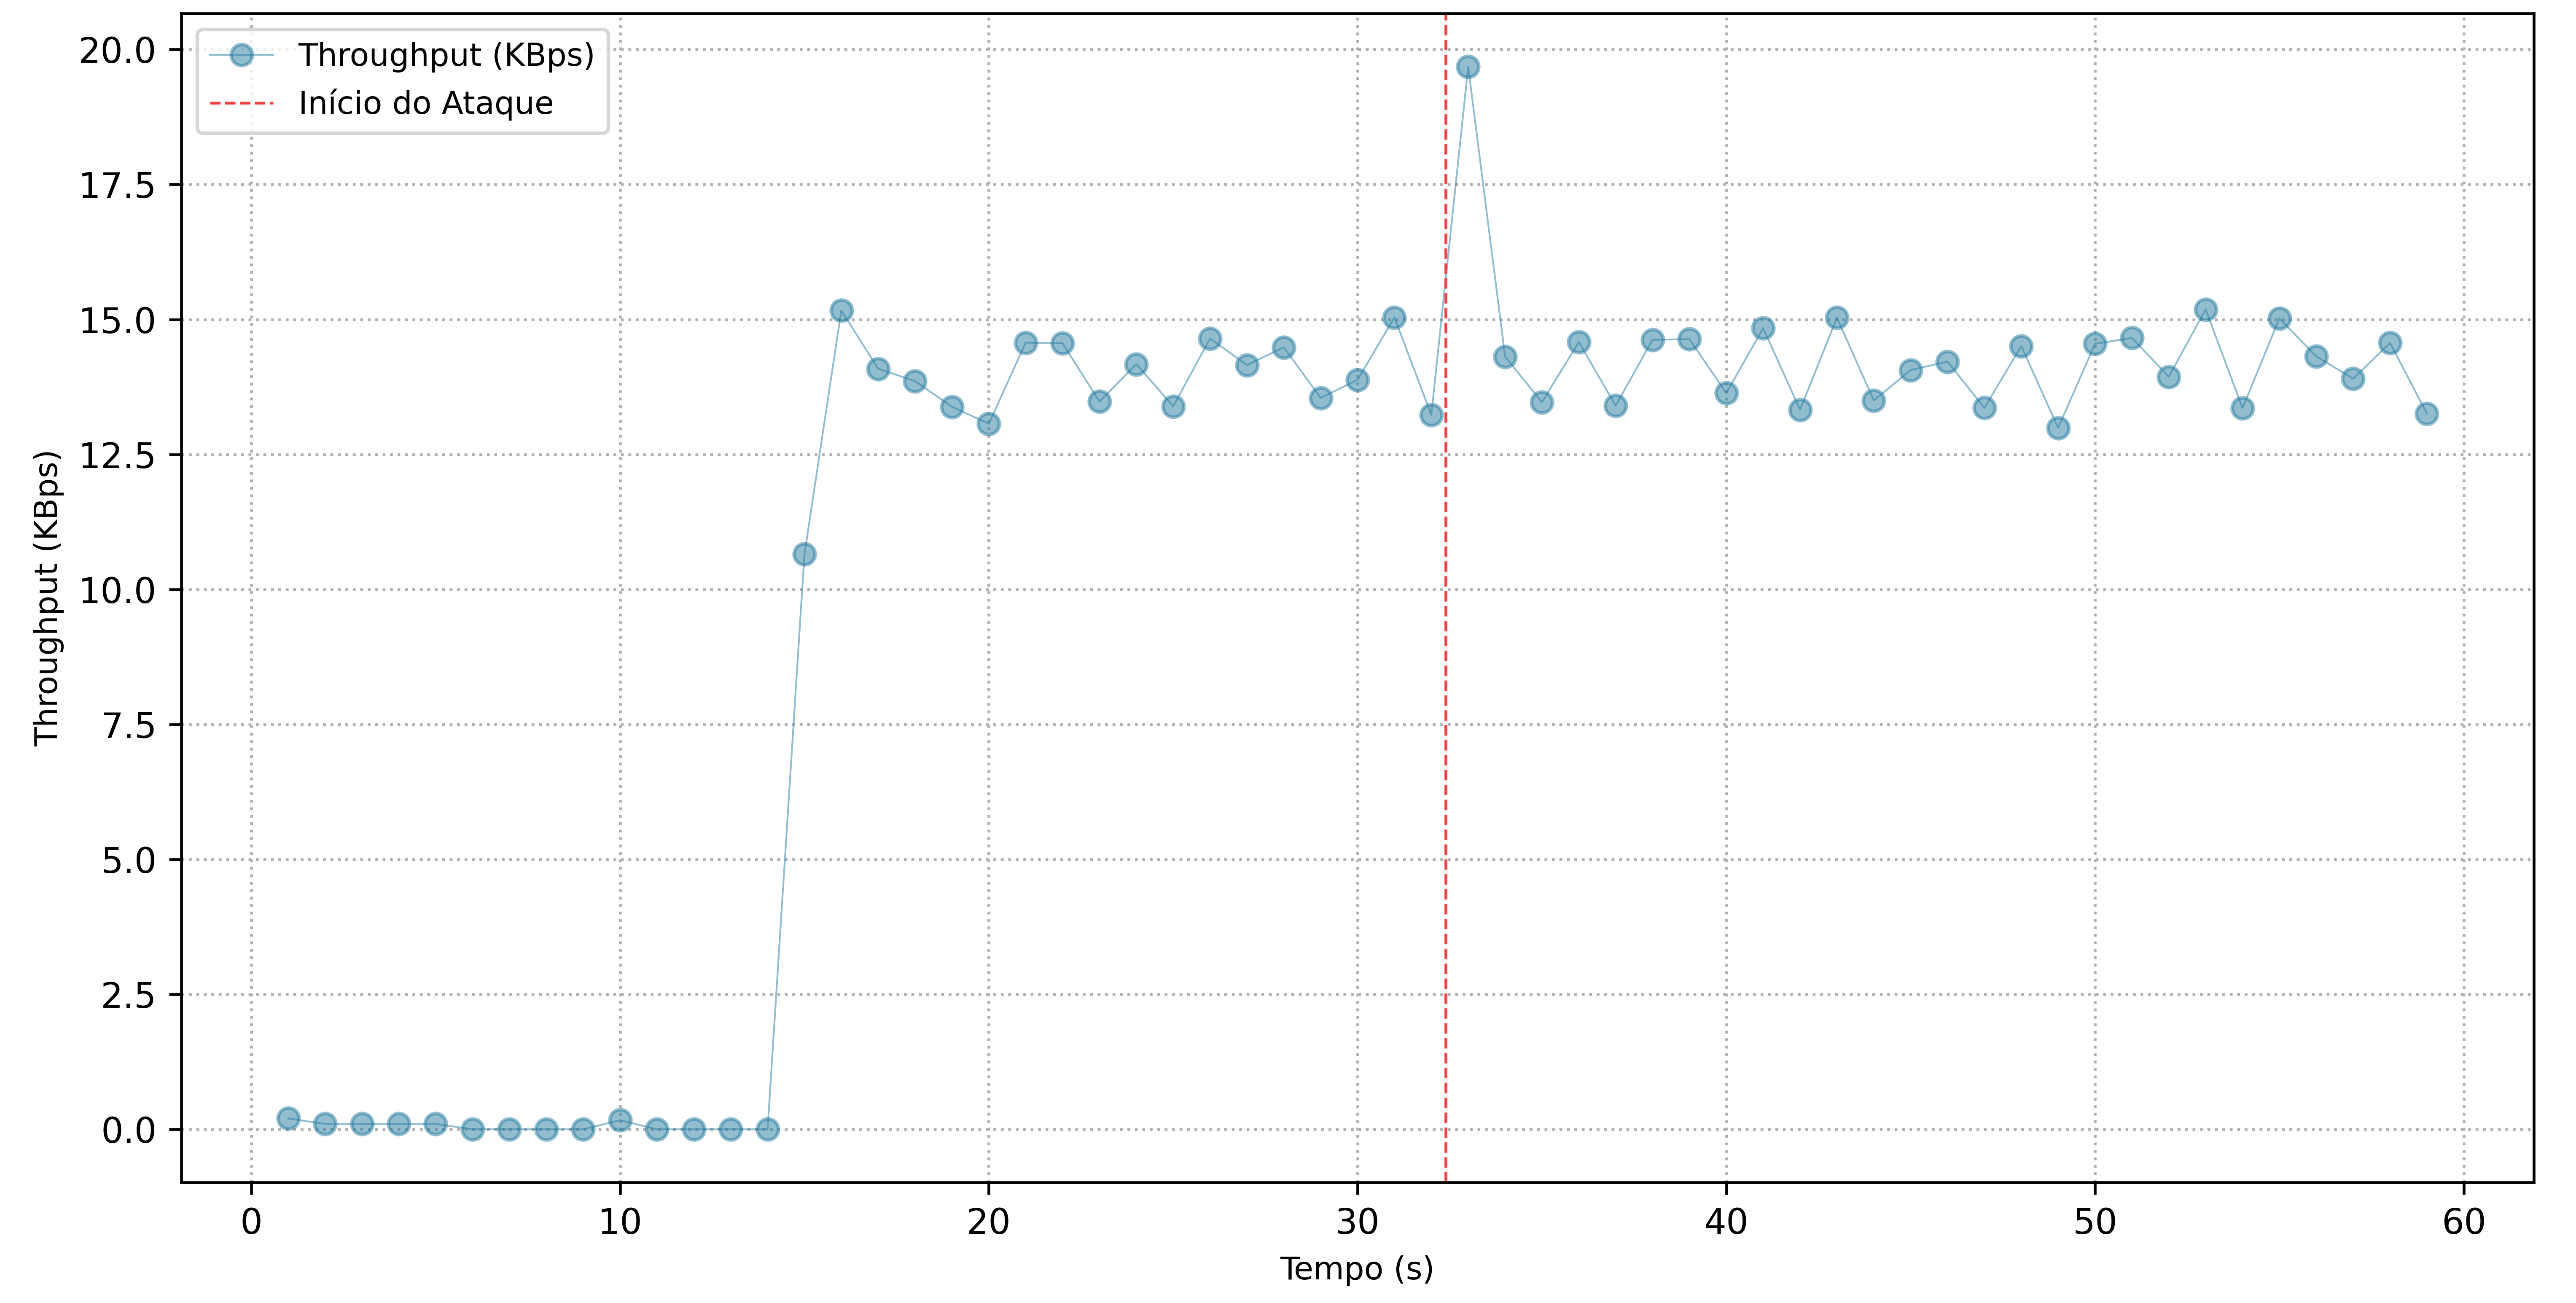
\includegraphics[width=1\textwidth, height=120pt]{USPSC-img/output/cropped/2-dos_certificate_inf_chain_loop-tput.png}
    \end{subfigure}%
    ~ 
    \begin{subfigure}[t]{0.5\textwidth}
        \centering
        \caption{Desempenho}
        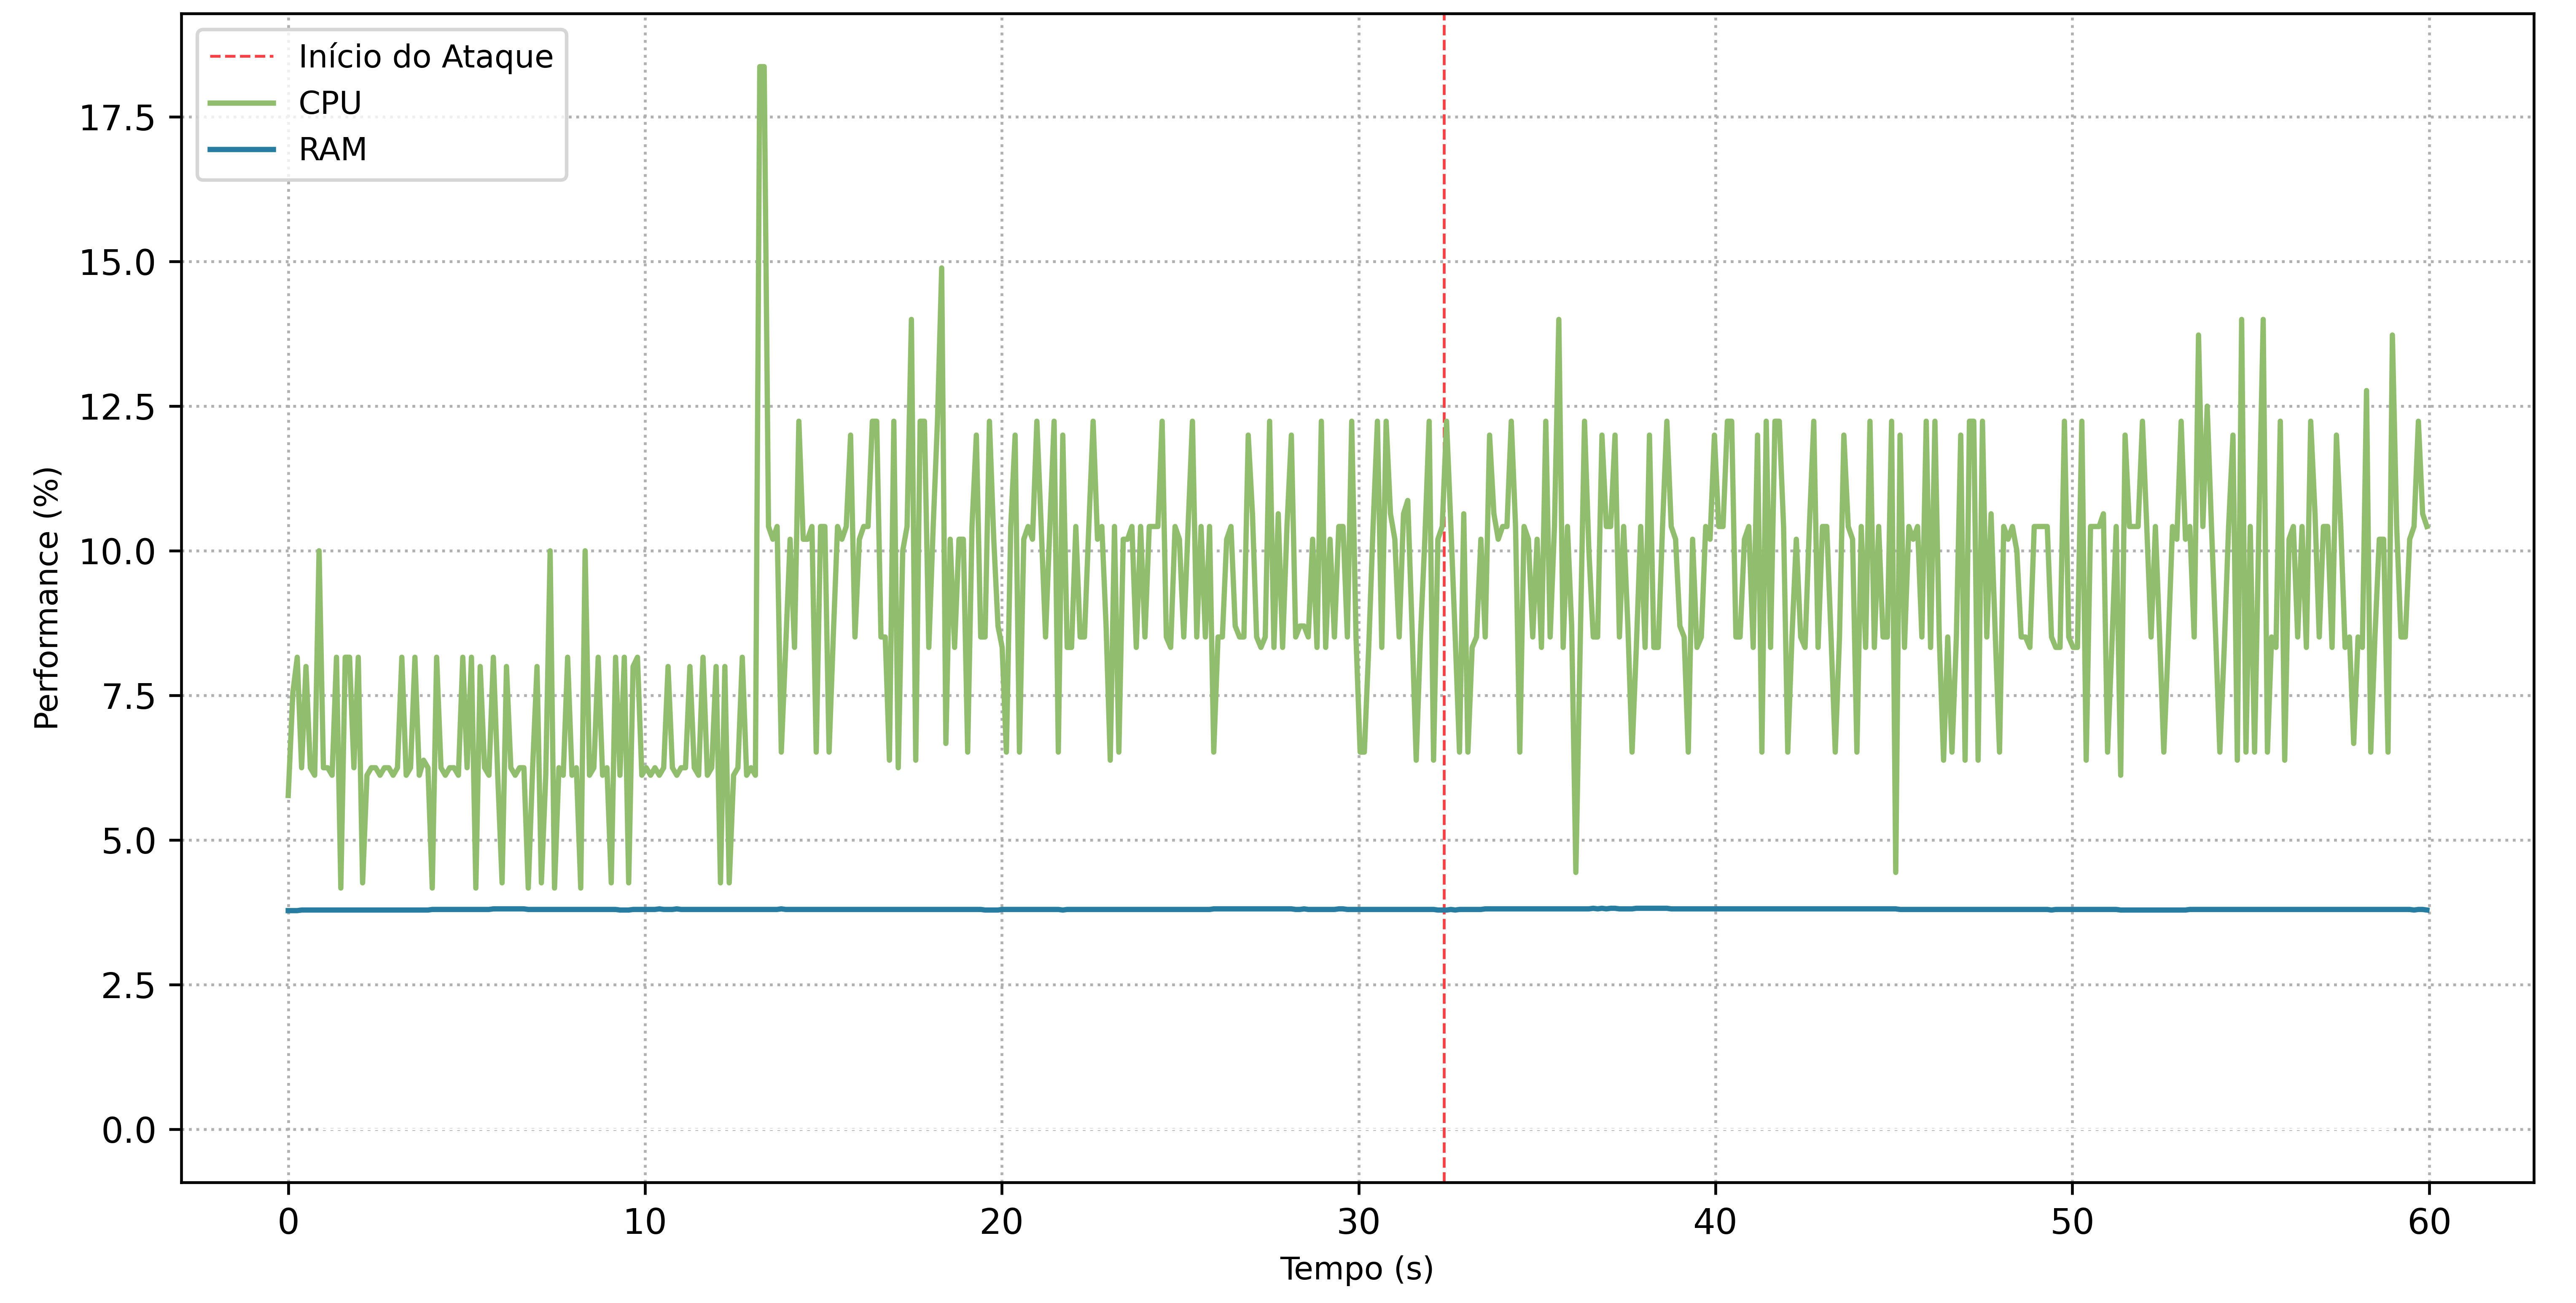
\includegraphics[width=1\textwidth, height=120pt]{USPSC-img/output/cropped/2-dos_certificate_inf_chain_loop-perf.png}
    \end{subfigure}%
    \\
    \begin{subfigure}[t]{0.5\textwidth}
        \centering
        \caption{Pacotes OPC UA}
        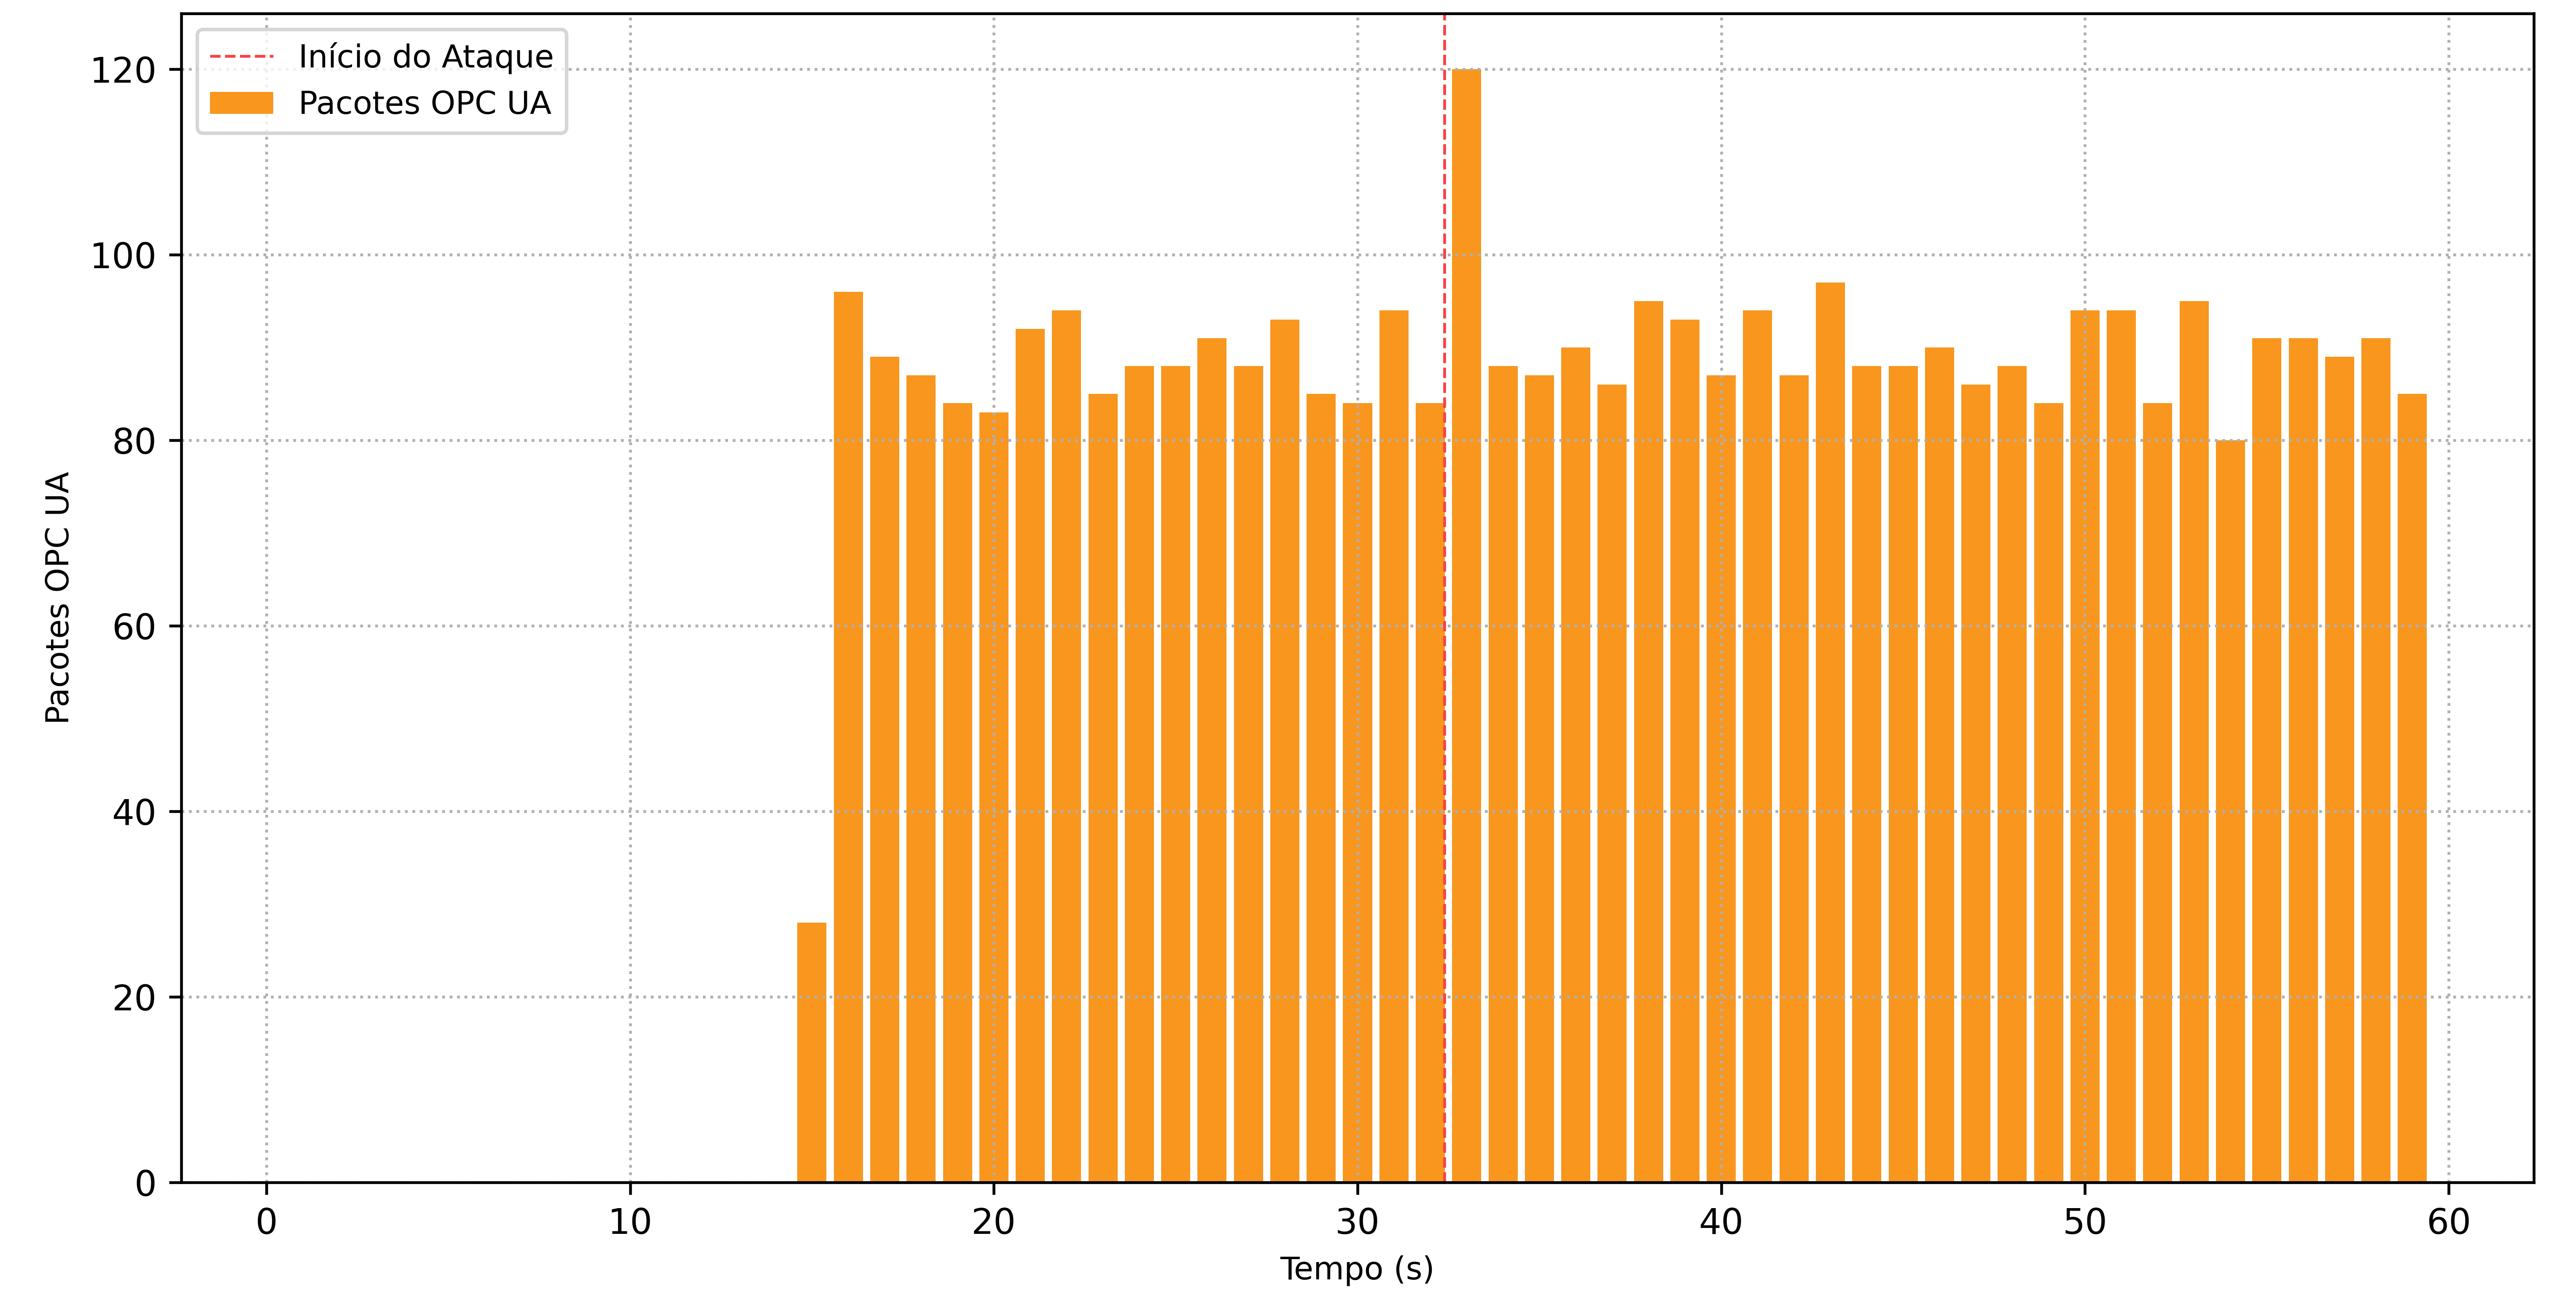
\includegraphics[width=1\textwidth, height=120pt]{USPSC-img/output/cropped/2-dos_certificate_inf_chain_loop-pack.png}
    \end{subfigure}%
    ~
    \begin{subfigure}[t]{0.5\textwidth}
        \centering
        \caption{RTT por pacote}
        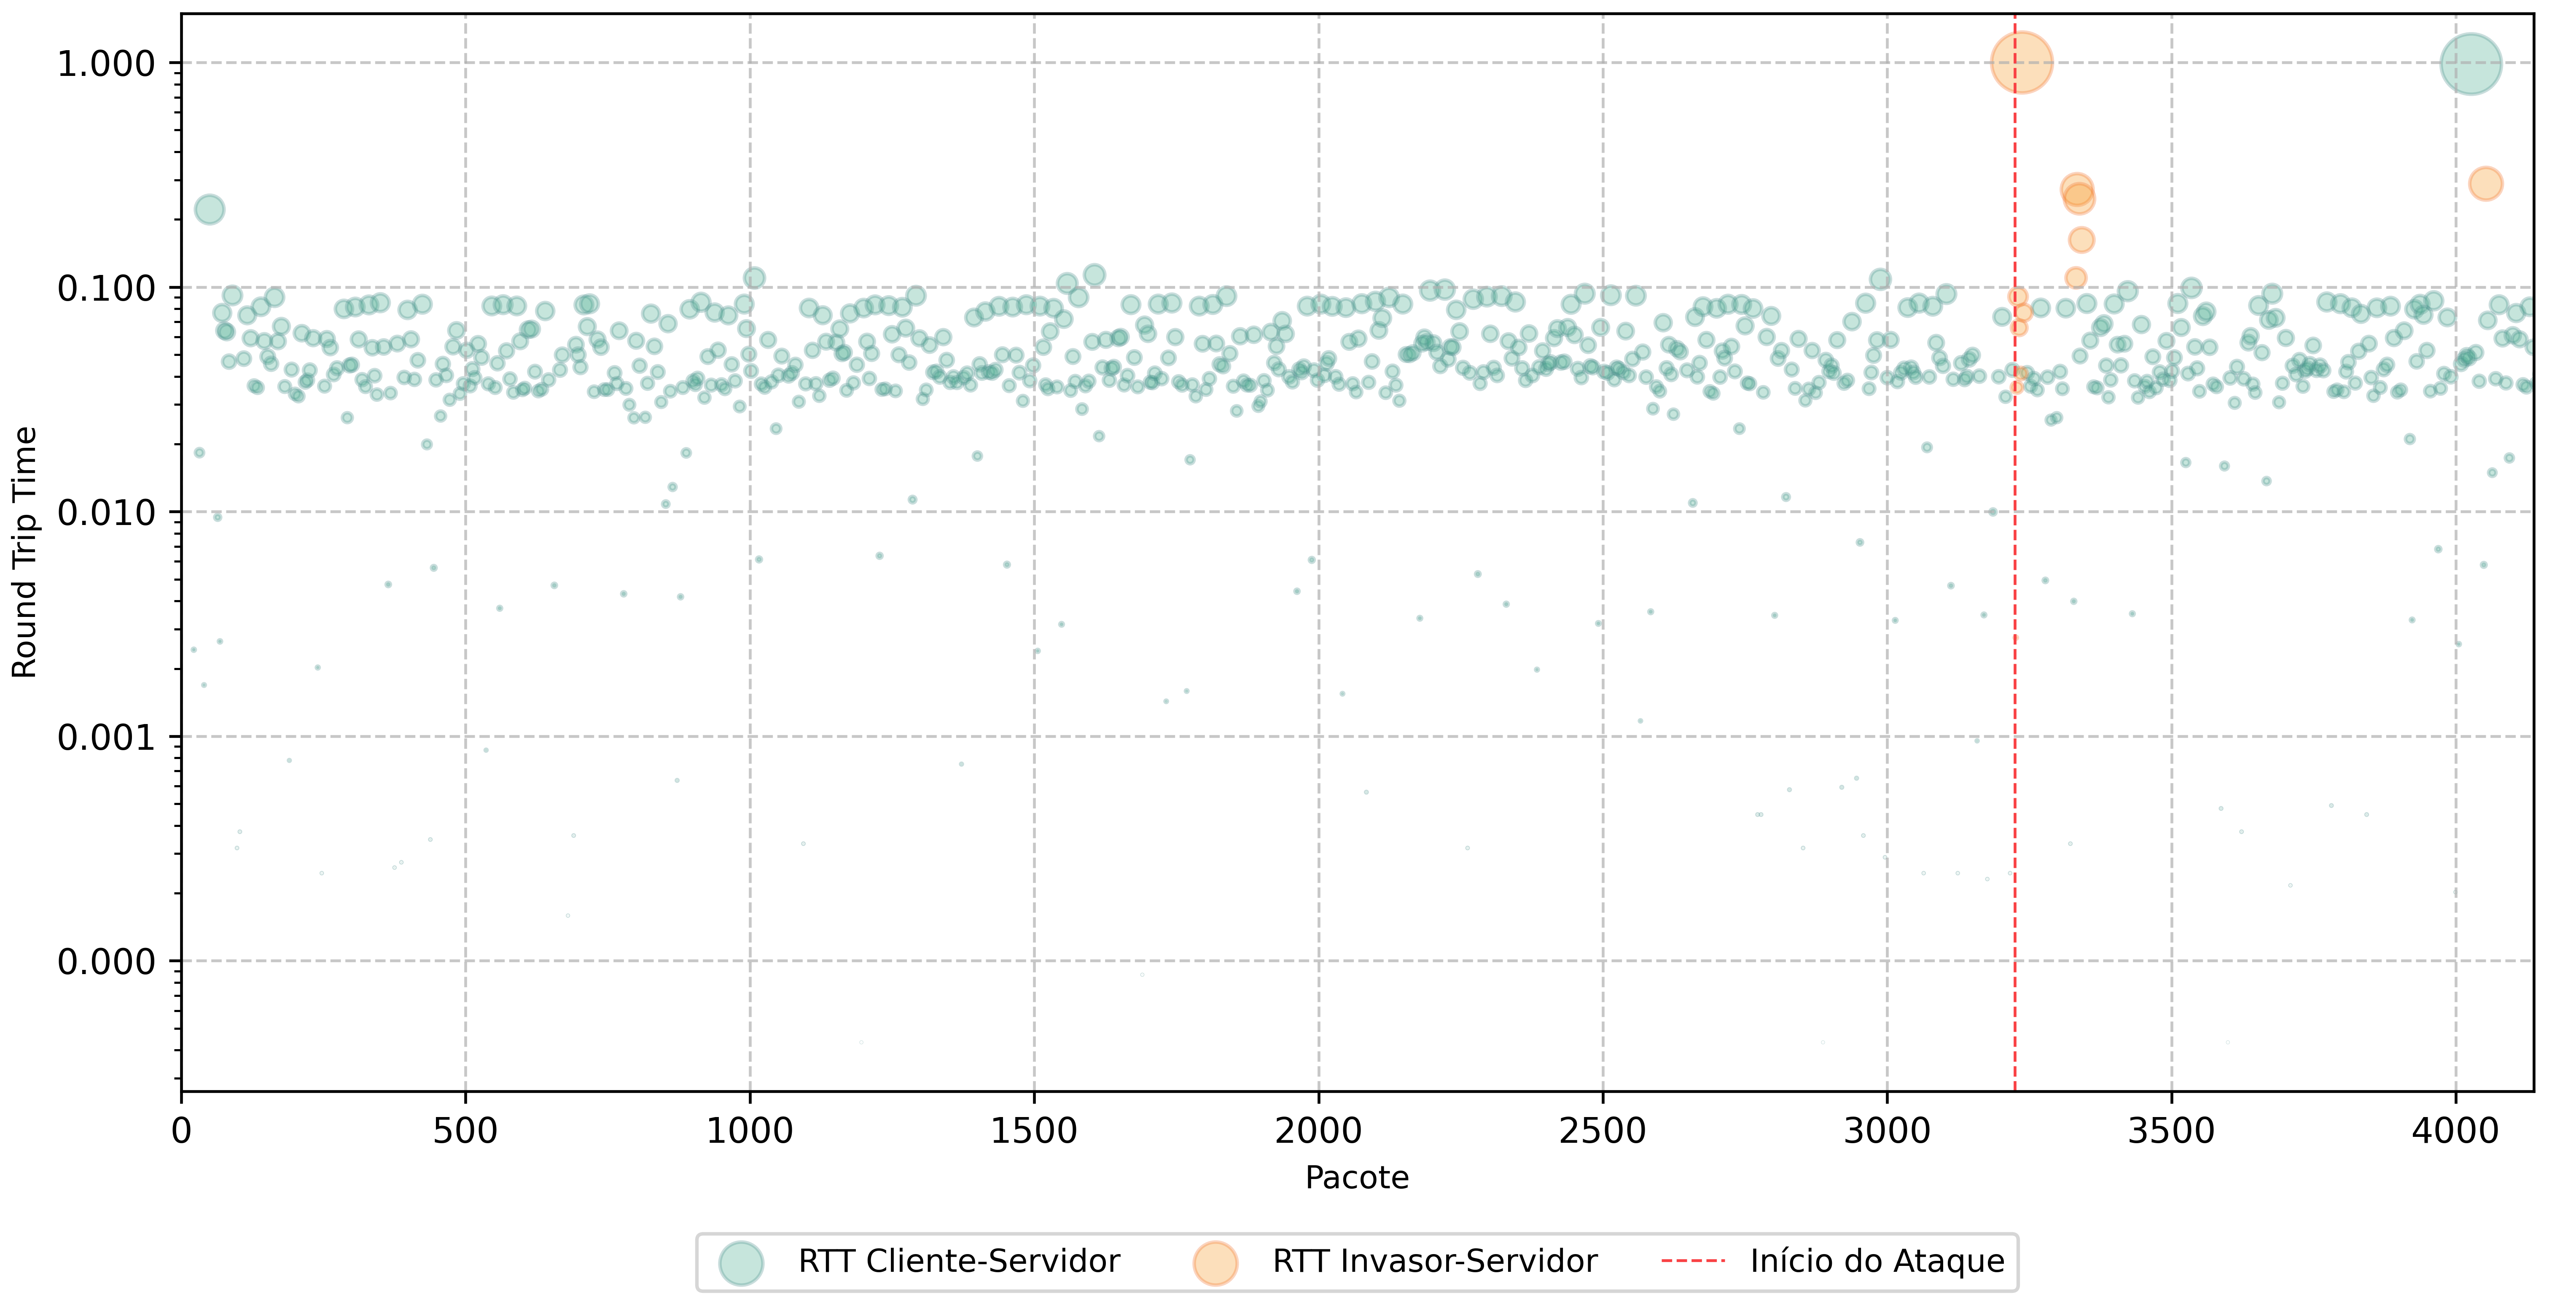
\includegraphics[width=1\textwidth, height=120pt]{USPSC-img/output/cropped/2-dos_certificate_inf_chain_loop-rttp.png}
    \end{subfigure}%
    % ~
    % \begin{subfigure}[t]{0.5\textwidth}
    %     \centering
    %     \caption{RTT por segundos}
    %     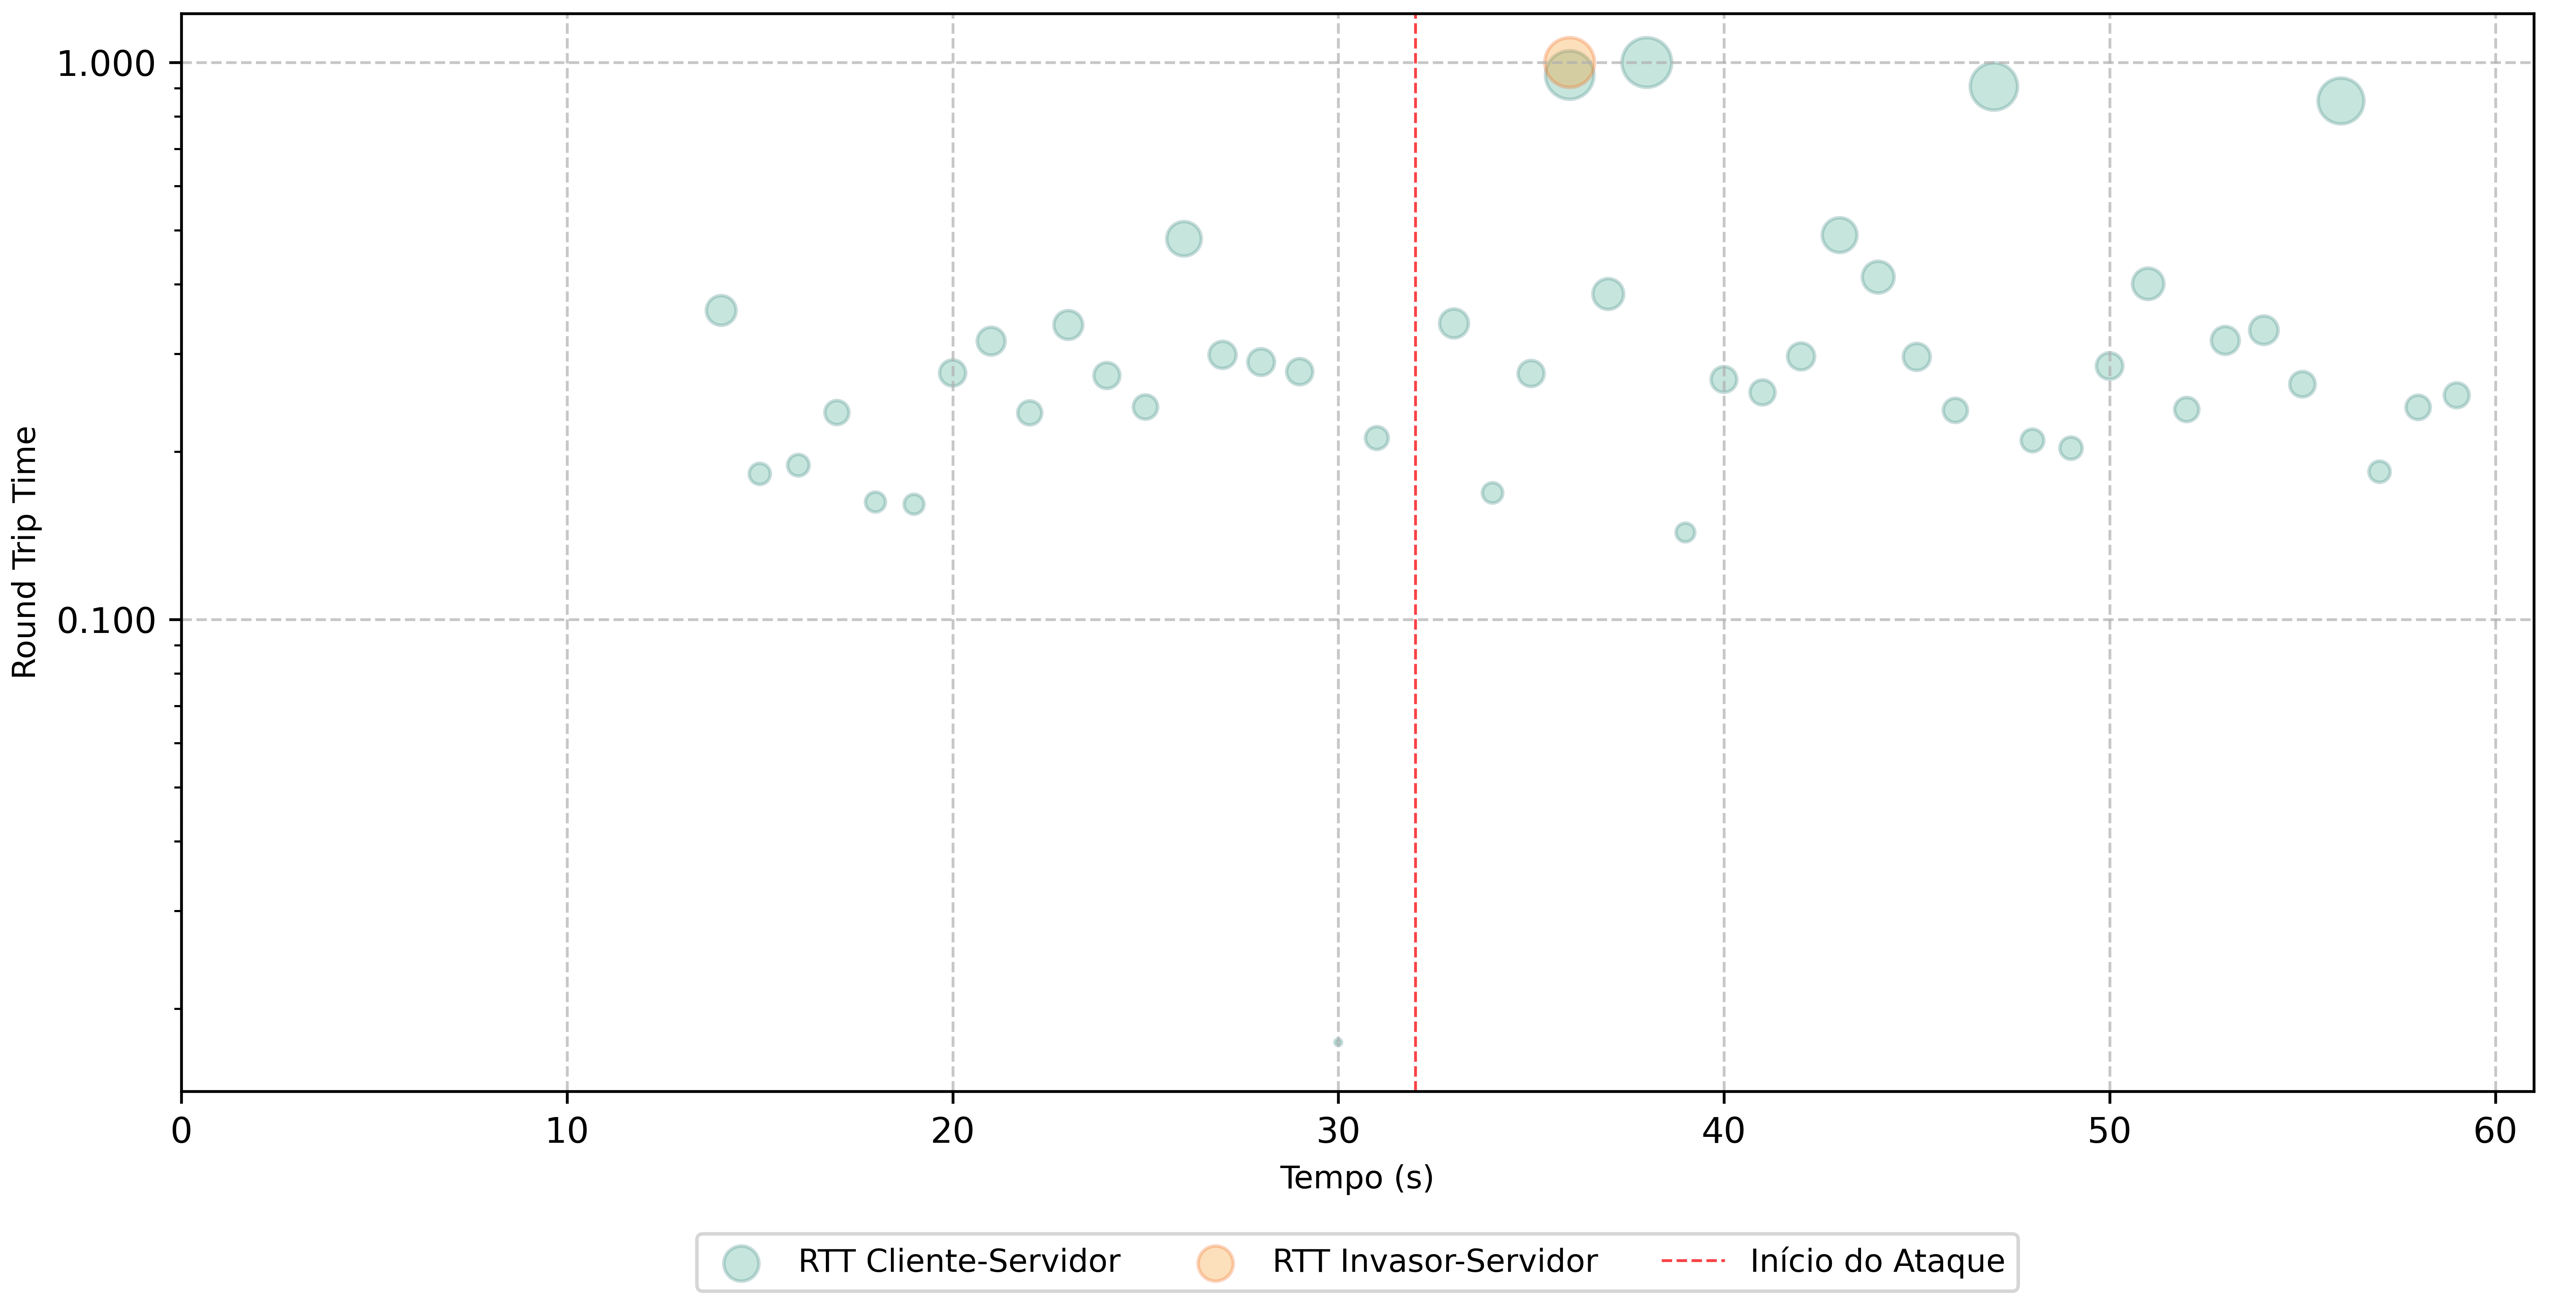
\includegraphics[width=1\textwidth, height=120pt]{USPSC-img/output/cropped/2-dos_certificate_inf_chain_loop-rtts.png}
    % \end{subfigure}%
\end{figure}

\begin{figure}[htbp!]
    \centering
    \caption{\label{fig:0-dos_function_call_null_deref}Gráficos do ataque de DoS pela chamada da função \textit{Dereference} nula - nível de segurança: `None'.}
    \begin{subfigure}[t]{0.5\textwidth}
        \centering
        \caption{\textit{Throughput}}
        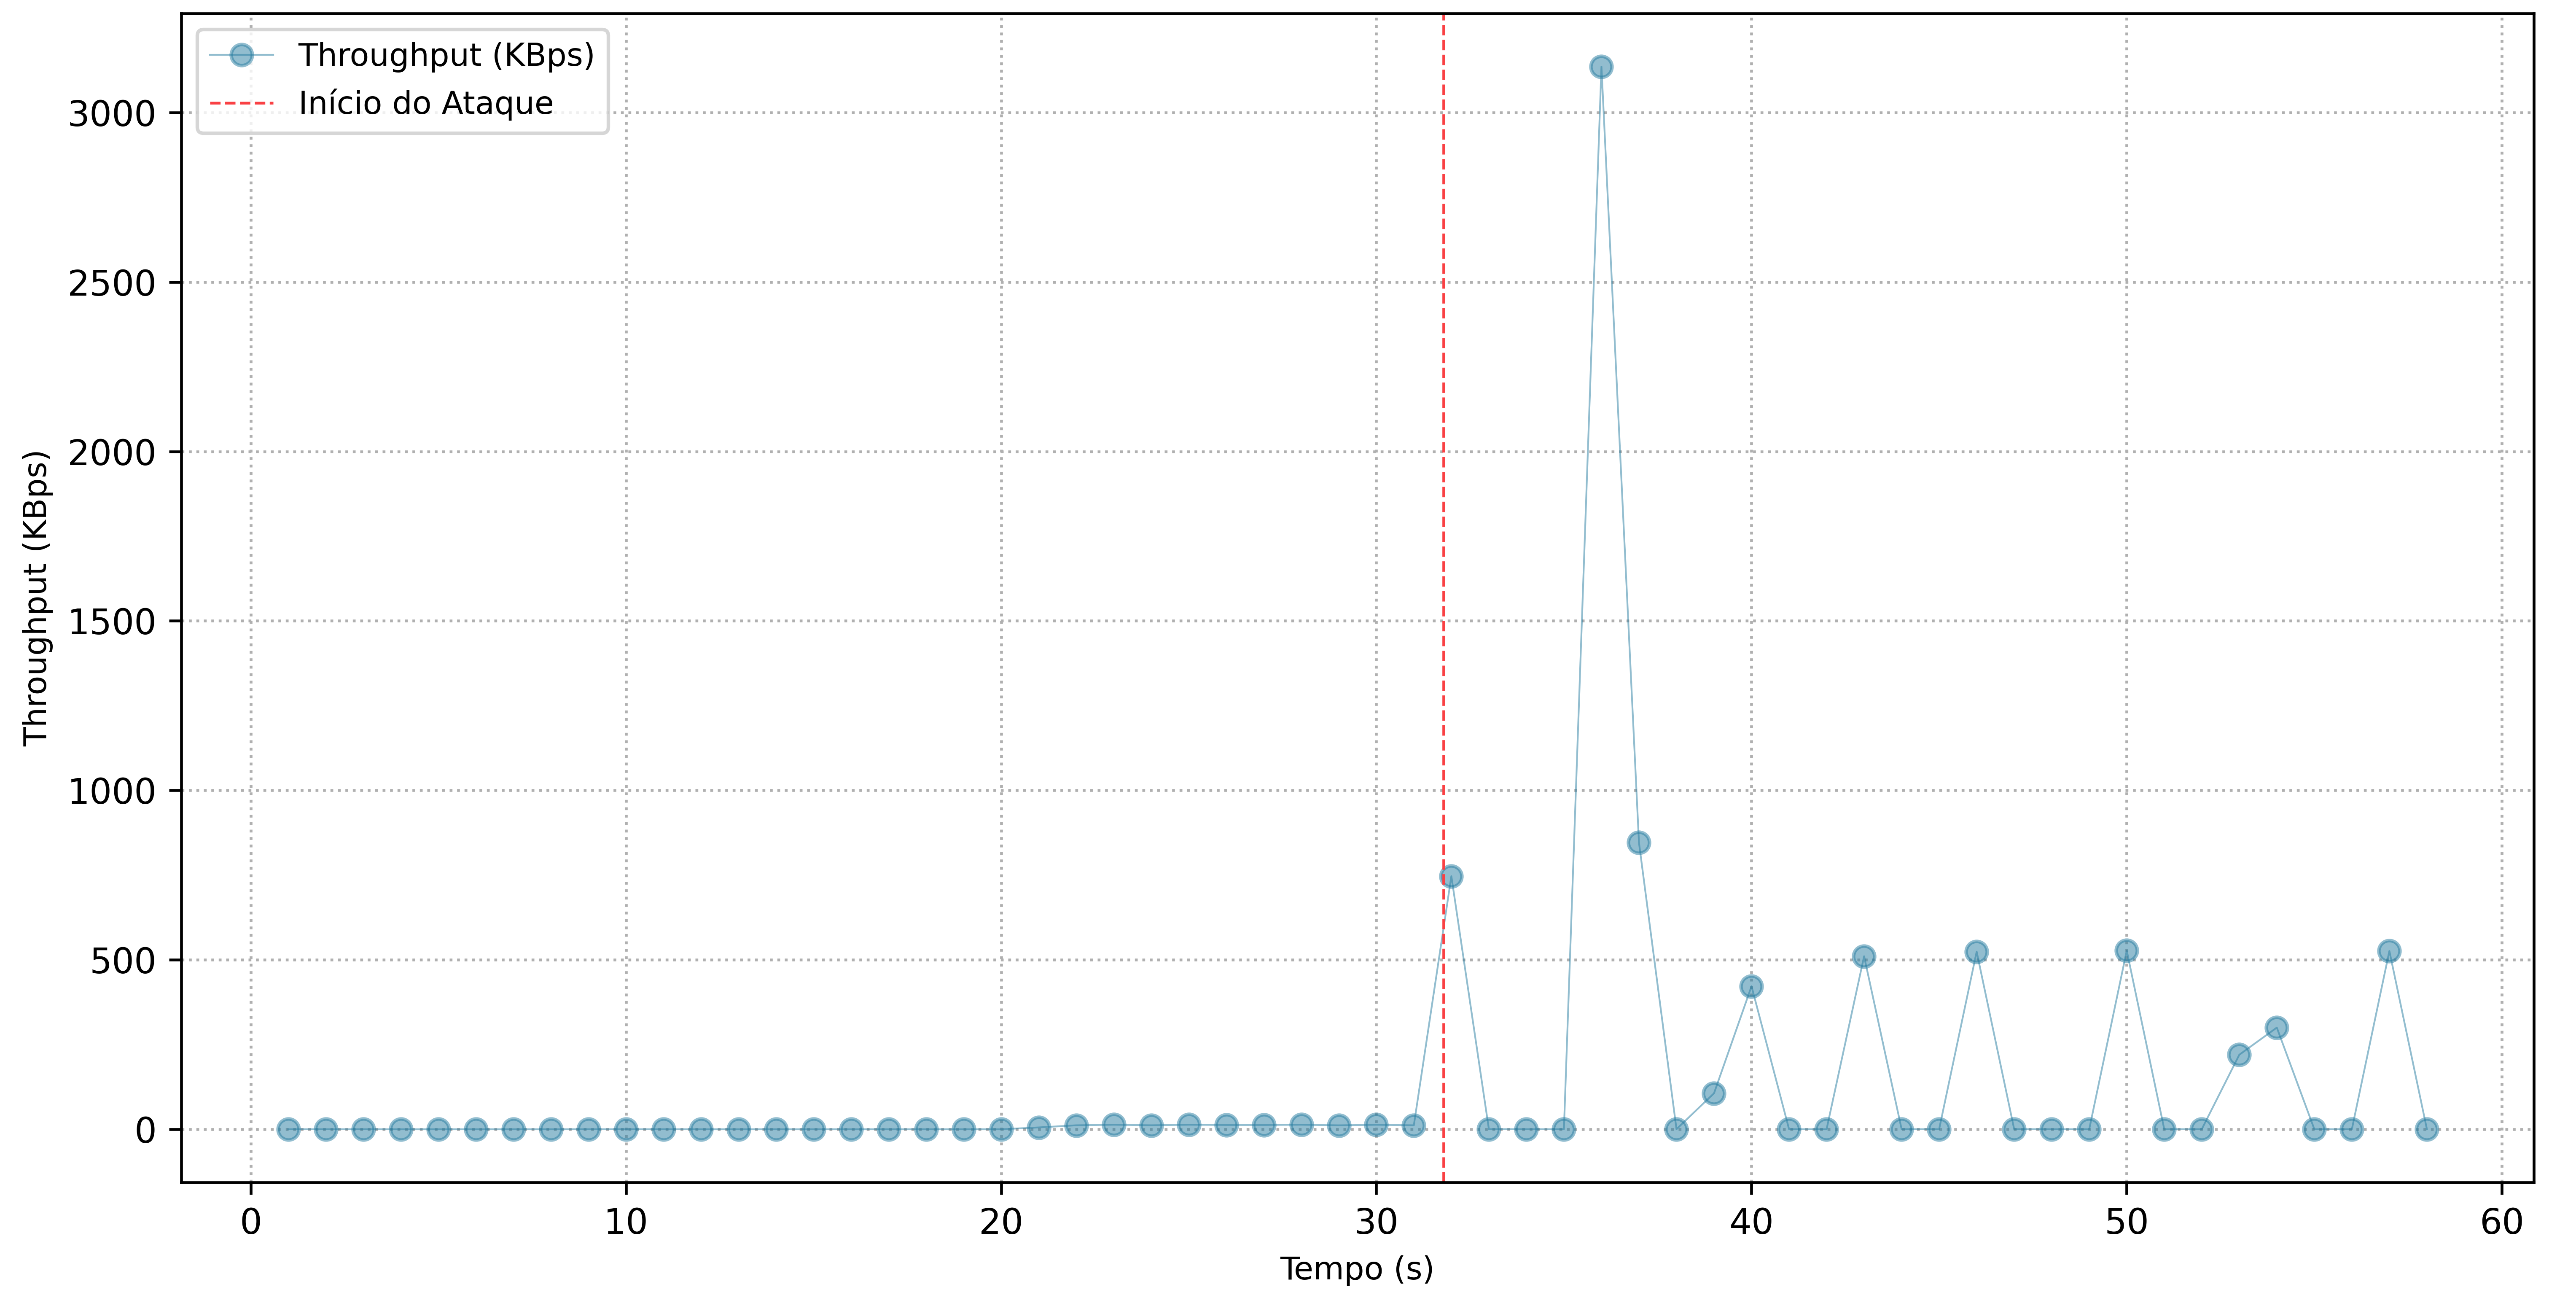
\includegraphics[width=1\textwidth, height=120pt]{USPSC-img/output/cropped/0-dos_function_call_null_deref-tput.png}
    \end{subfigure}%
    ~ 
    \begin{subfigure}[t]{0.5\textwidth}
        \centering
        \caption{Desempenho}
        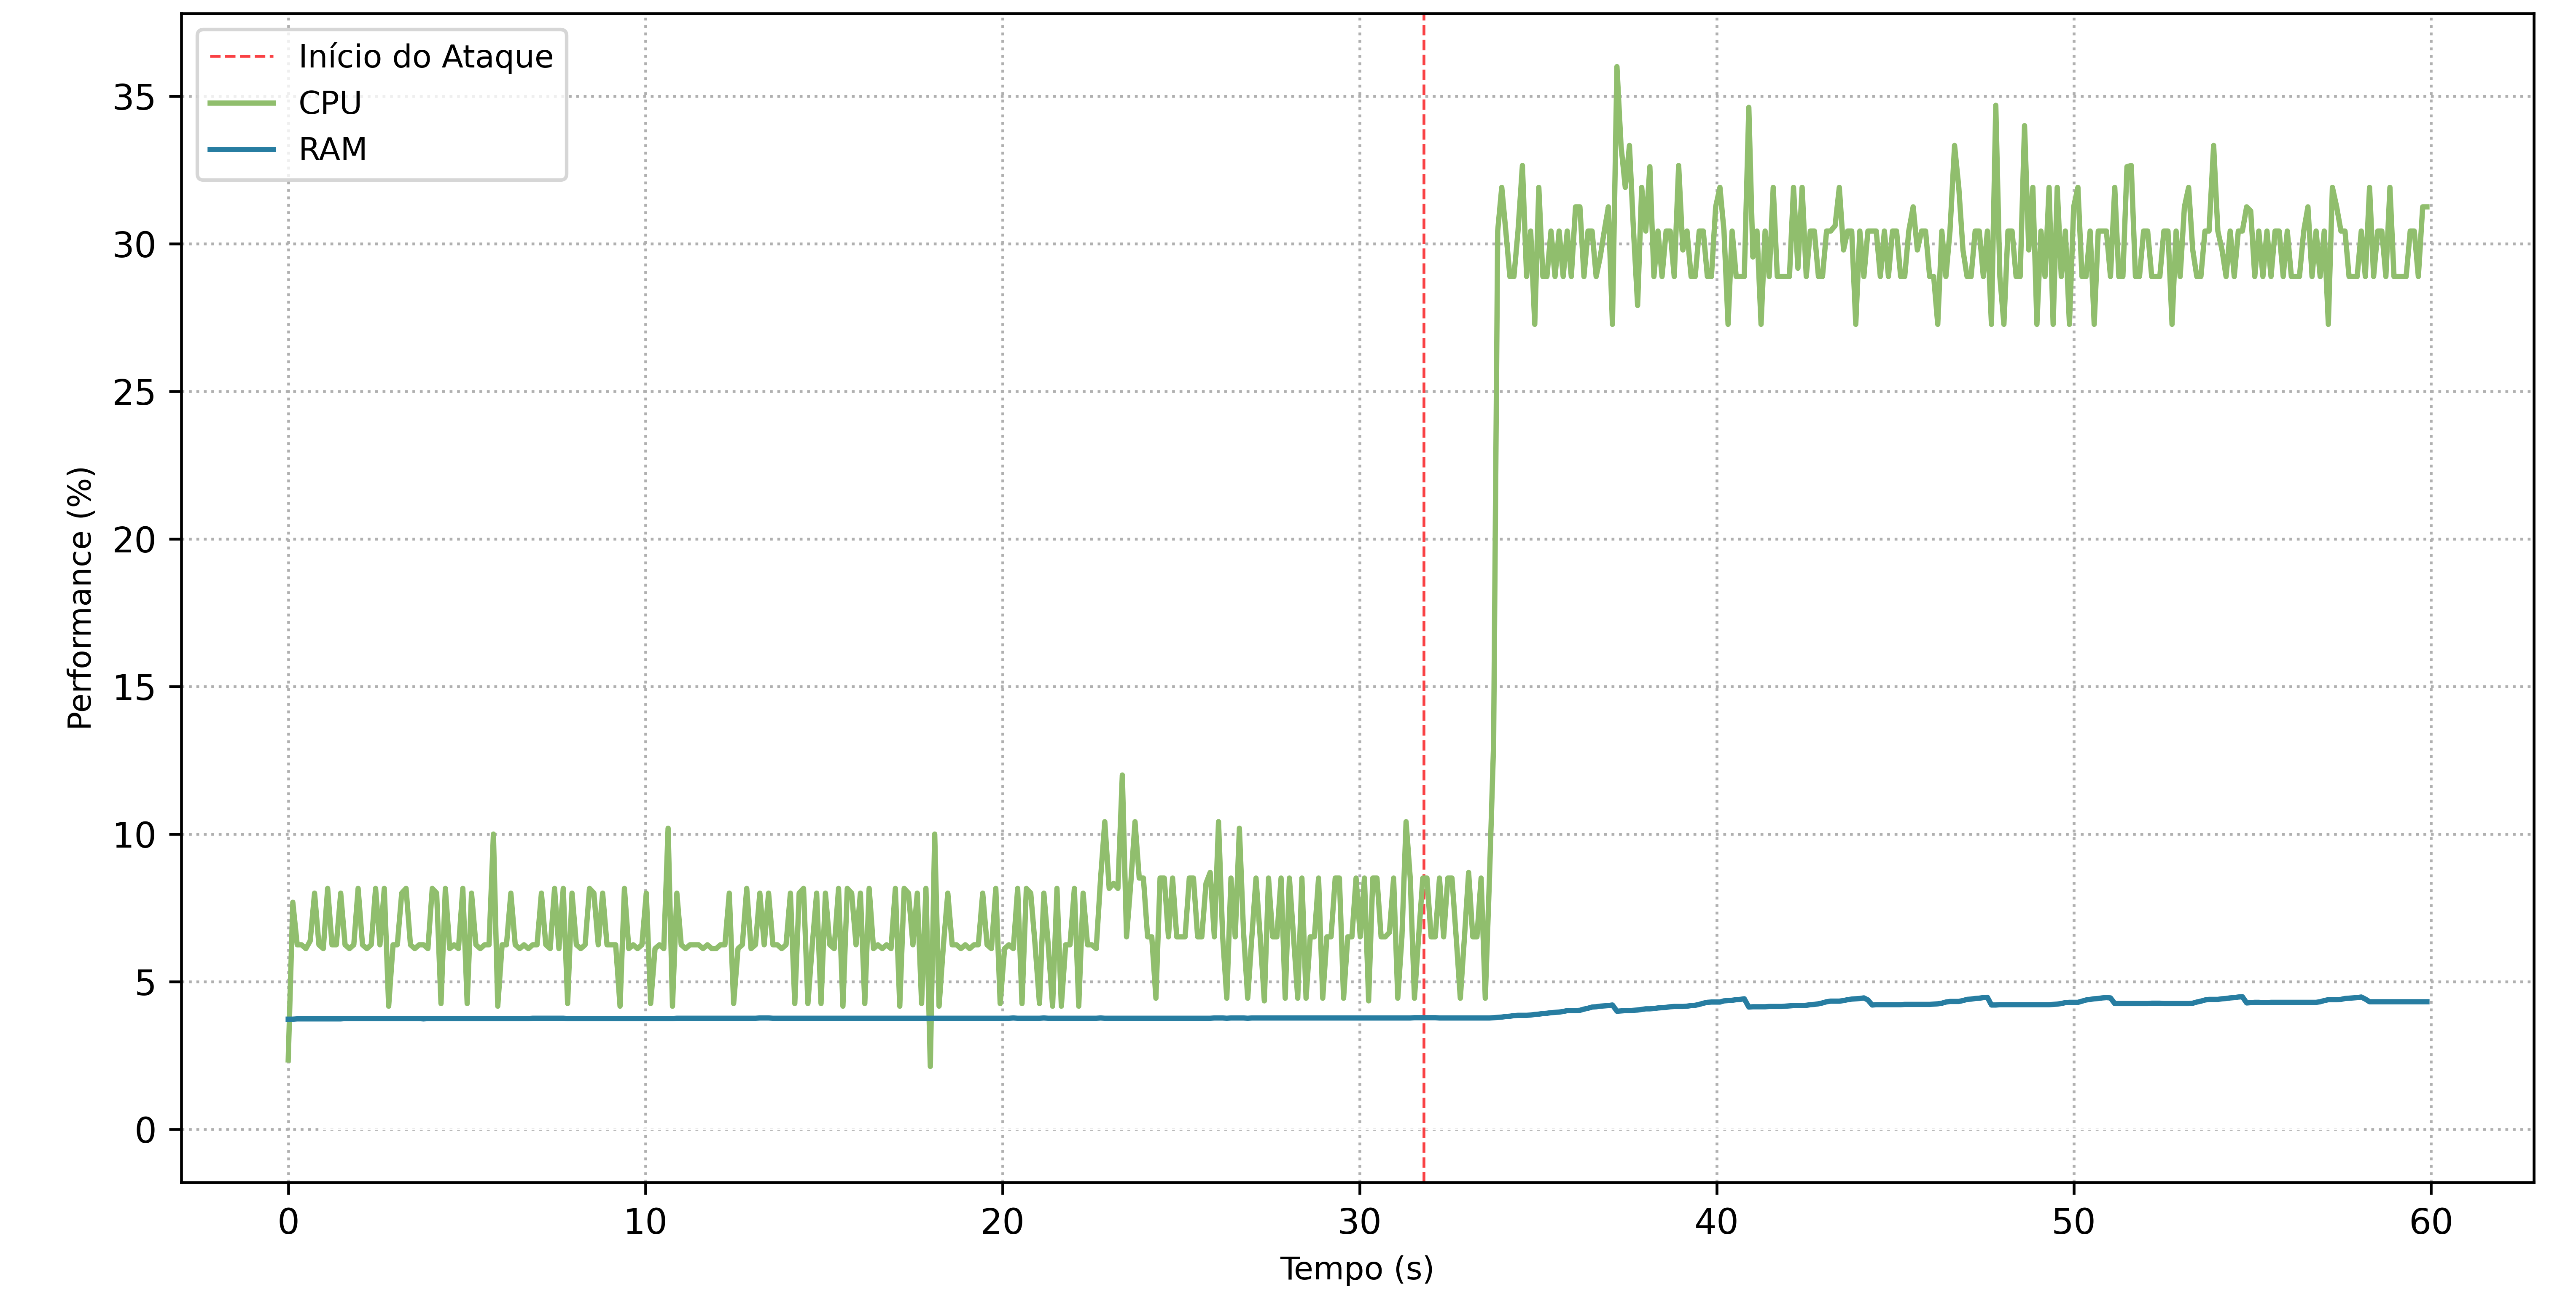
\includegraphics[width=1\textwidth, height=120pt]{USPSC-img/output/cropped/0-dos_function_call_null_deref-perf.png}
    \end{subfigure}%
    \\
    \begin{subfigure}[t]{0.5\textwidth}
        \centering
        \caption{Pacotes OPC UA}
        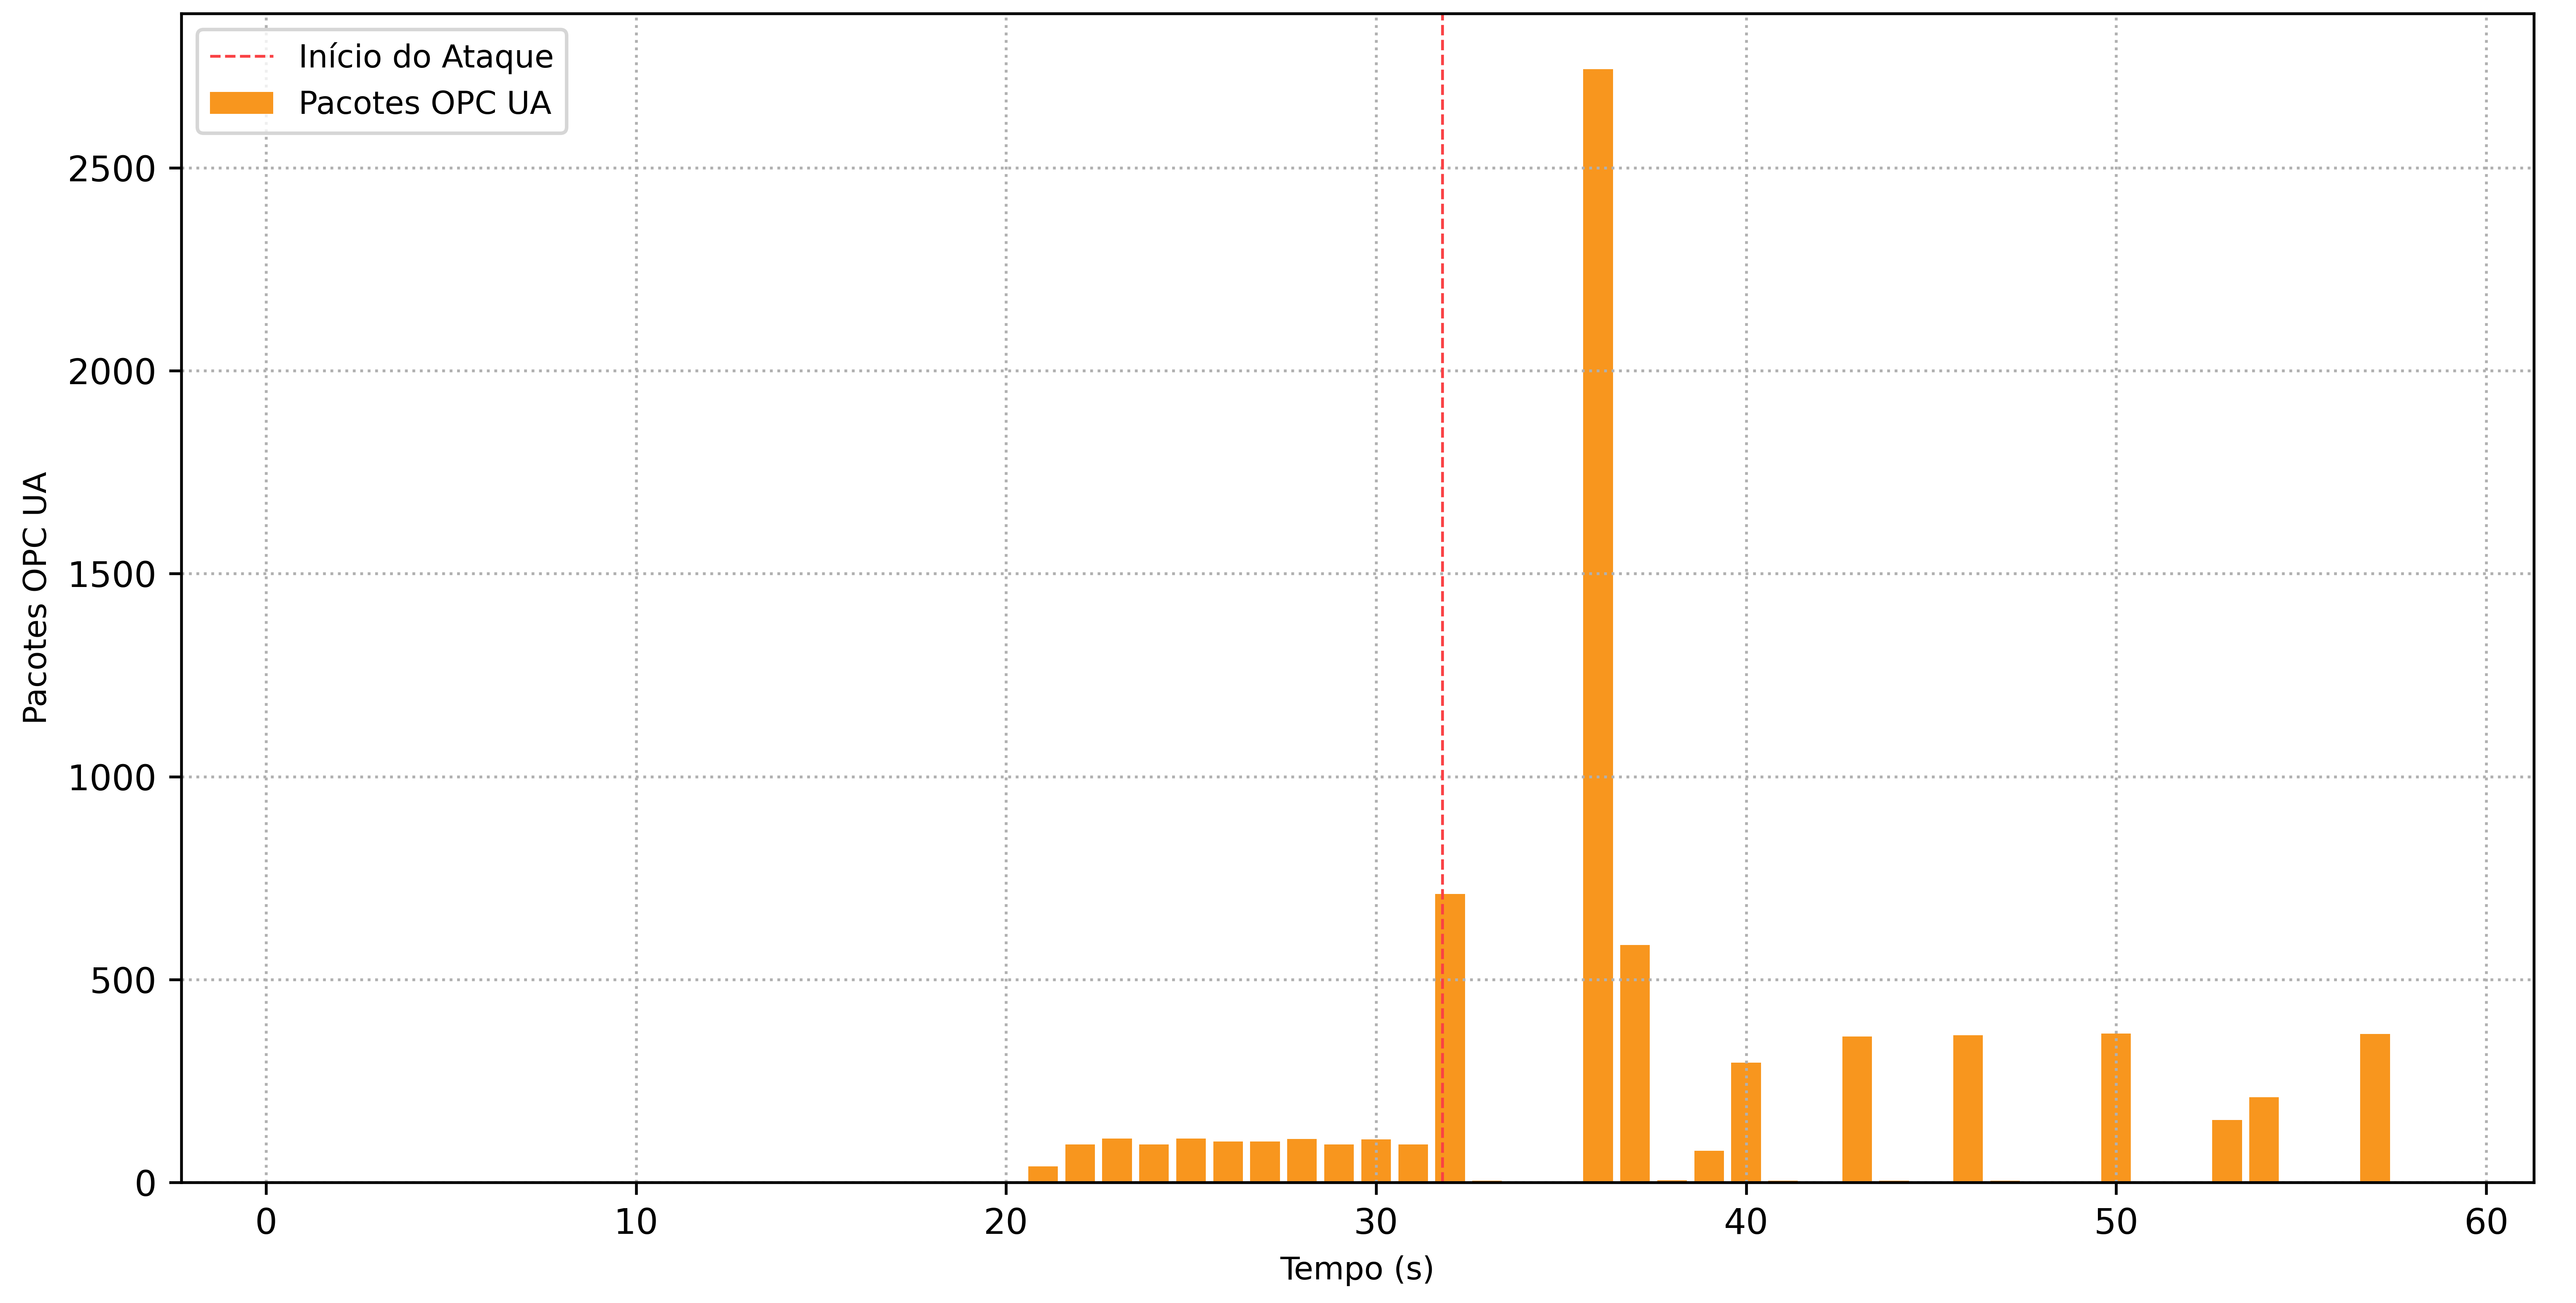
\includegraphics[width=1\textwidth, height=120pt]{USPSC-img/output/cropped/0-dos_function_call_null_deref-pack.png}
    \end{subfigure}%
    ~
    \begin{subfigure}[t]{0.5\textwidth}
        \centering
        \caption{RTT por pacote}
        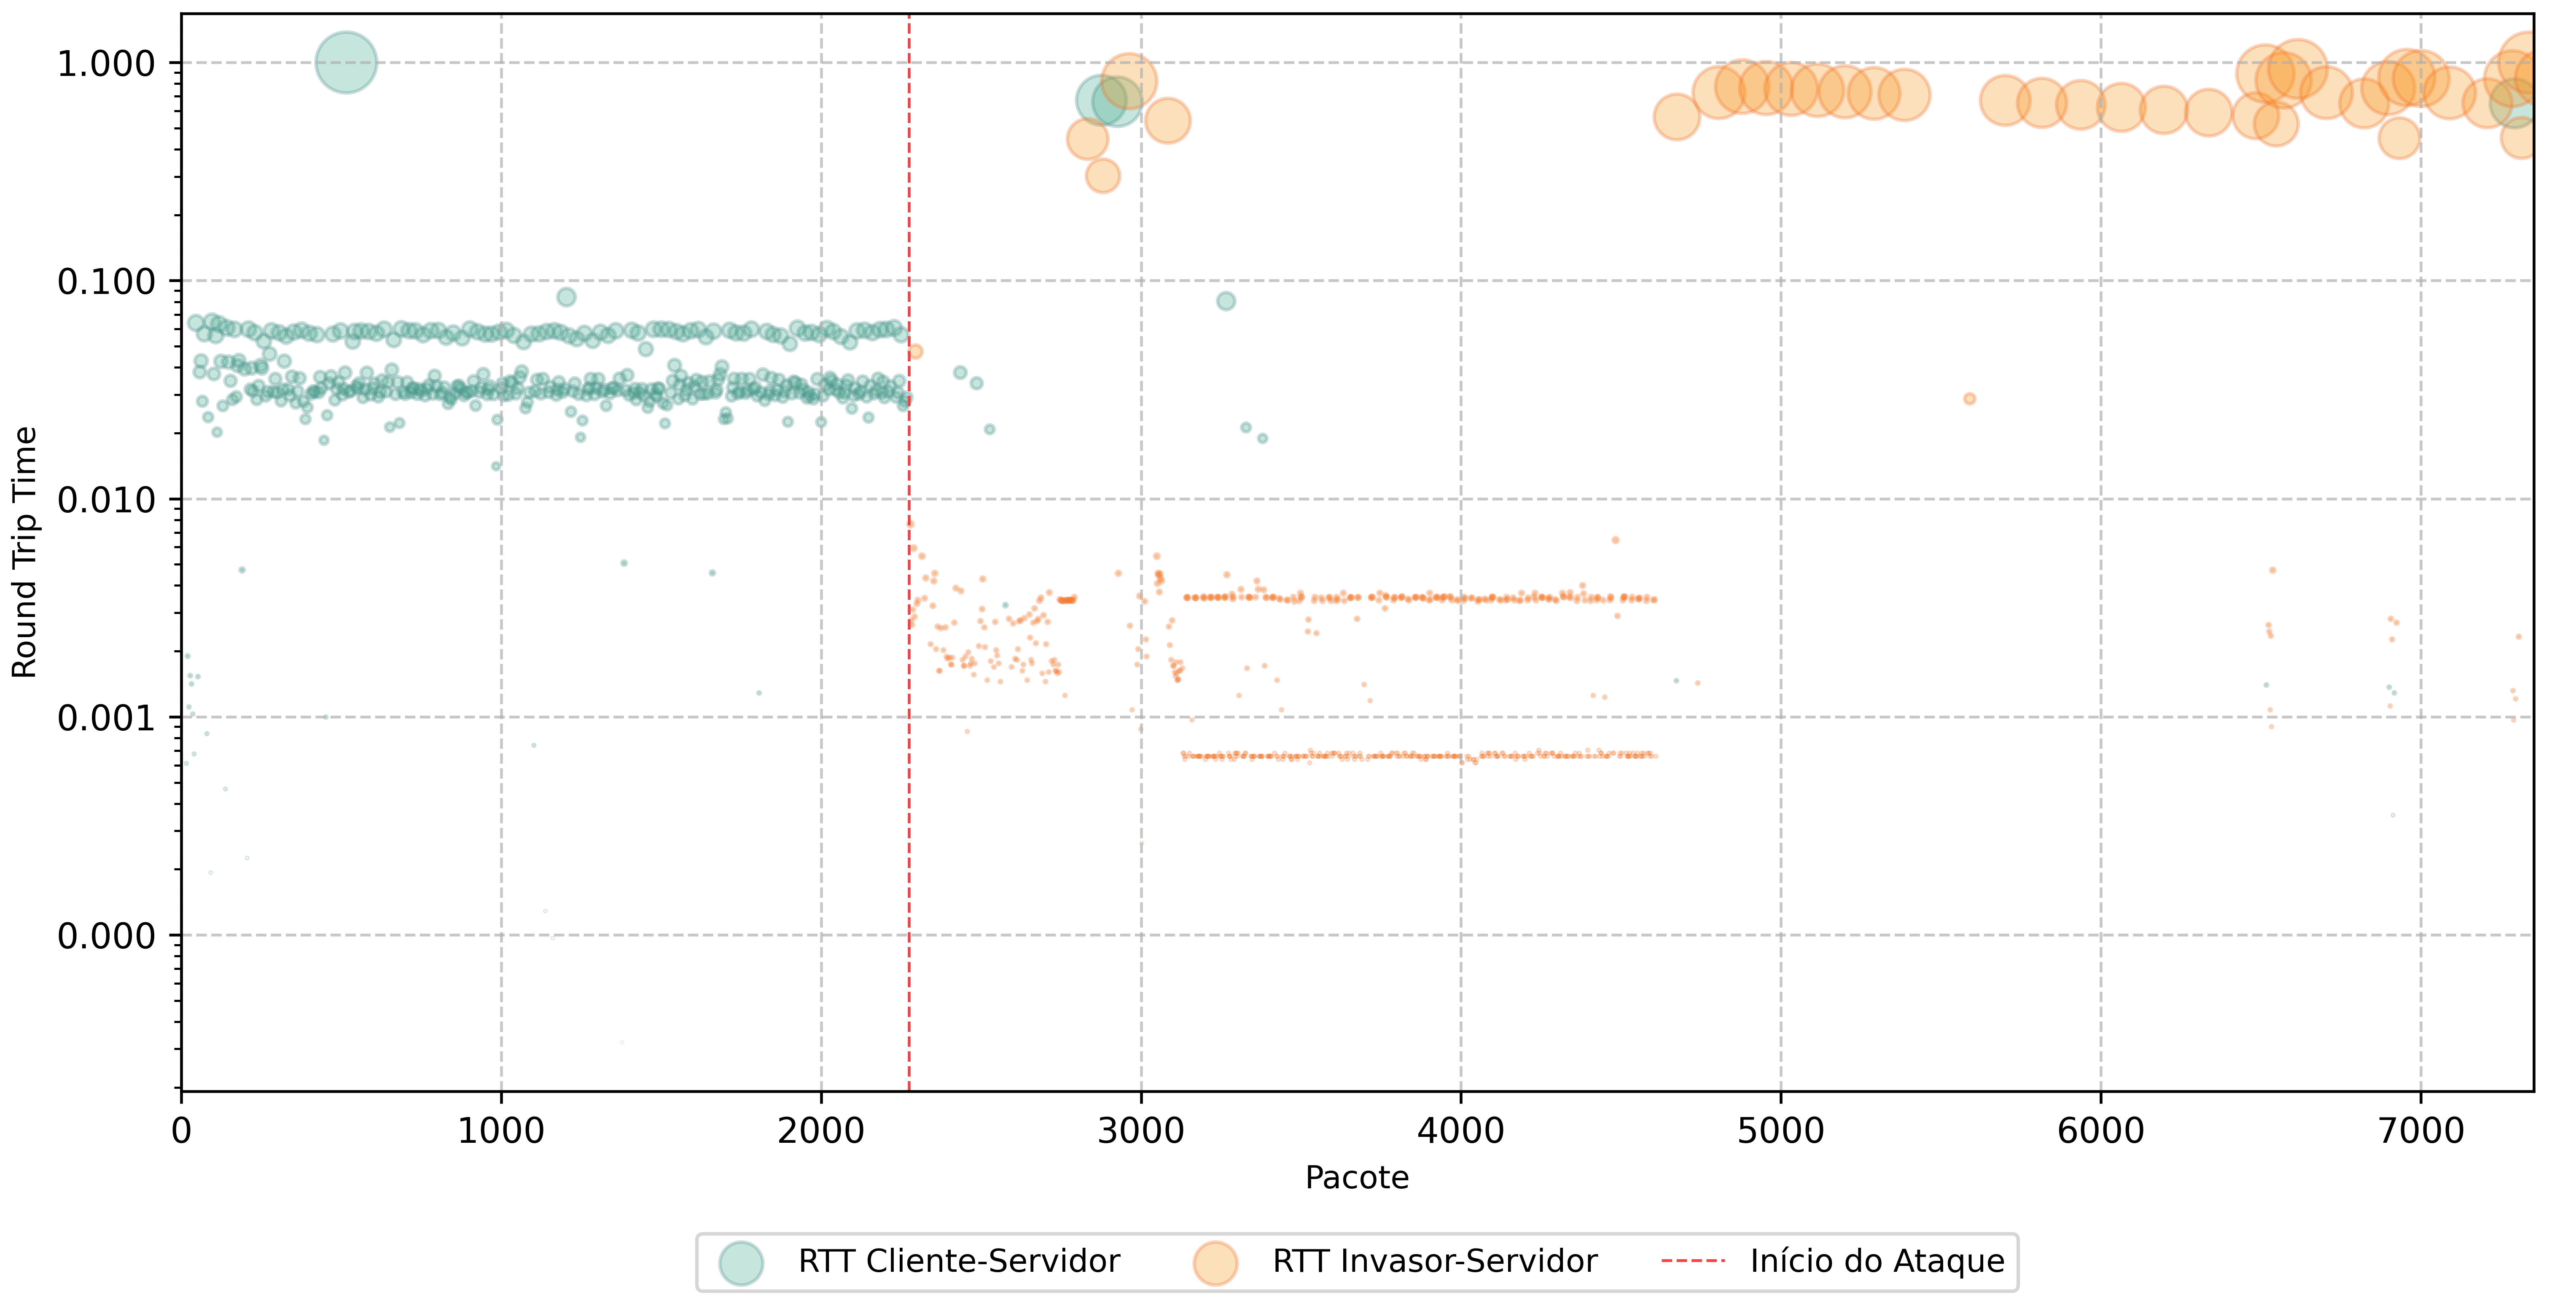
\includegraphics[width=1\textwidth, height=120pt]{USPSC-img/output/cropped/0-dos_function_call_null_deref-rttp.png}
    \end{subfigure}%
    % ~
    % \begin{subfigure}[t]{0.5\textwidth}
    %     \centering
    %     \caption{RTT por segundos}
    %     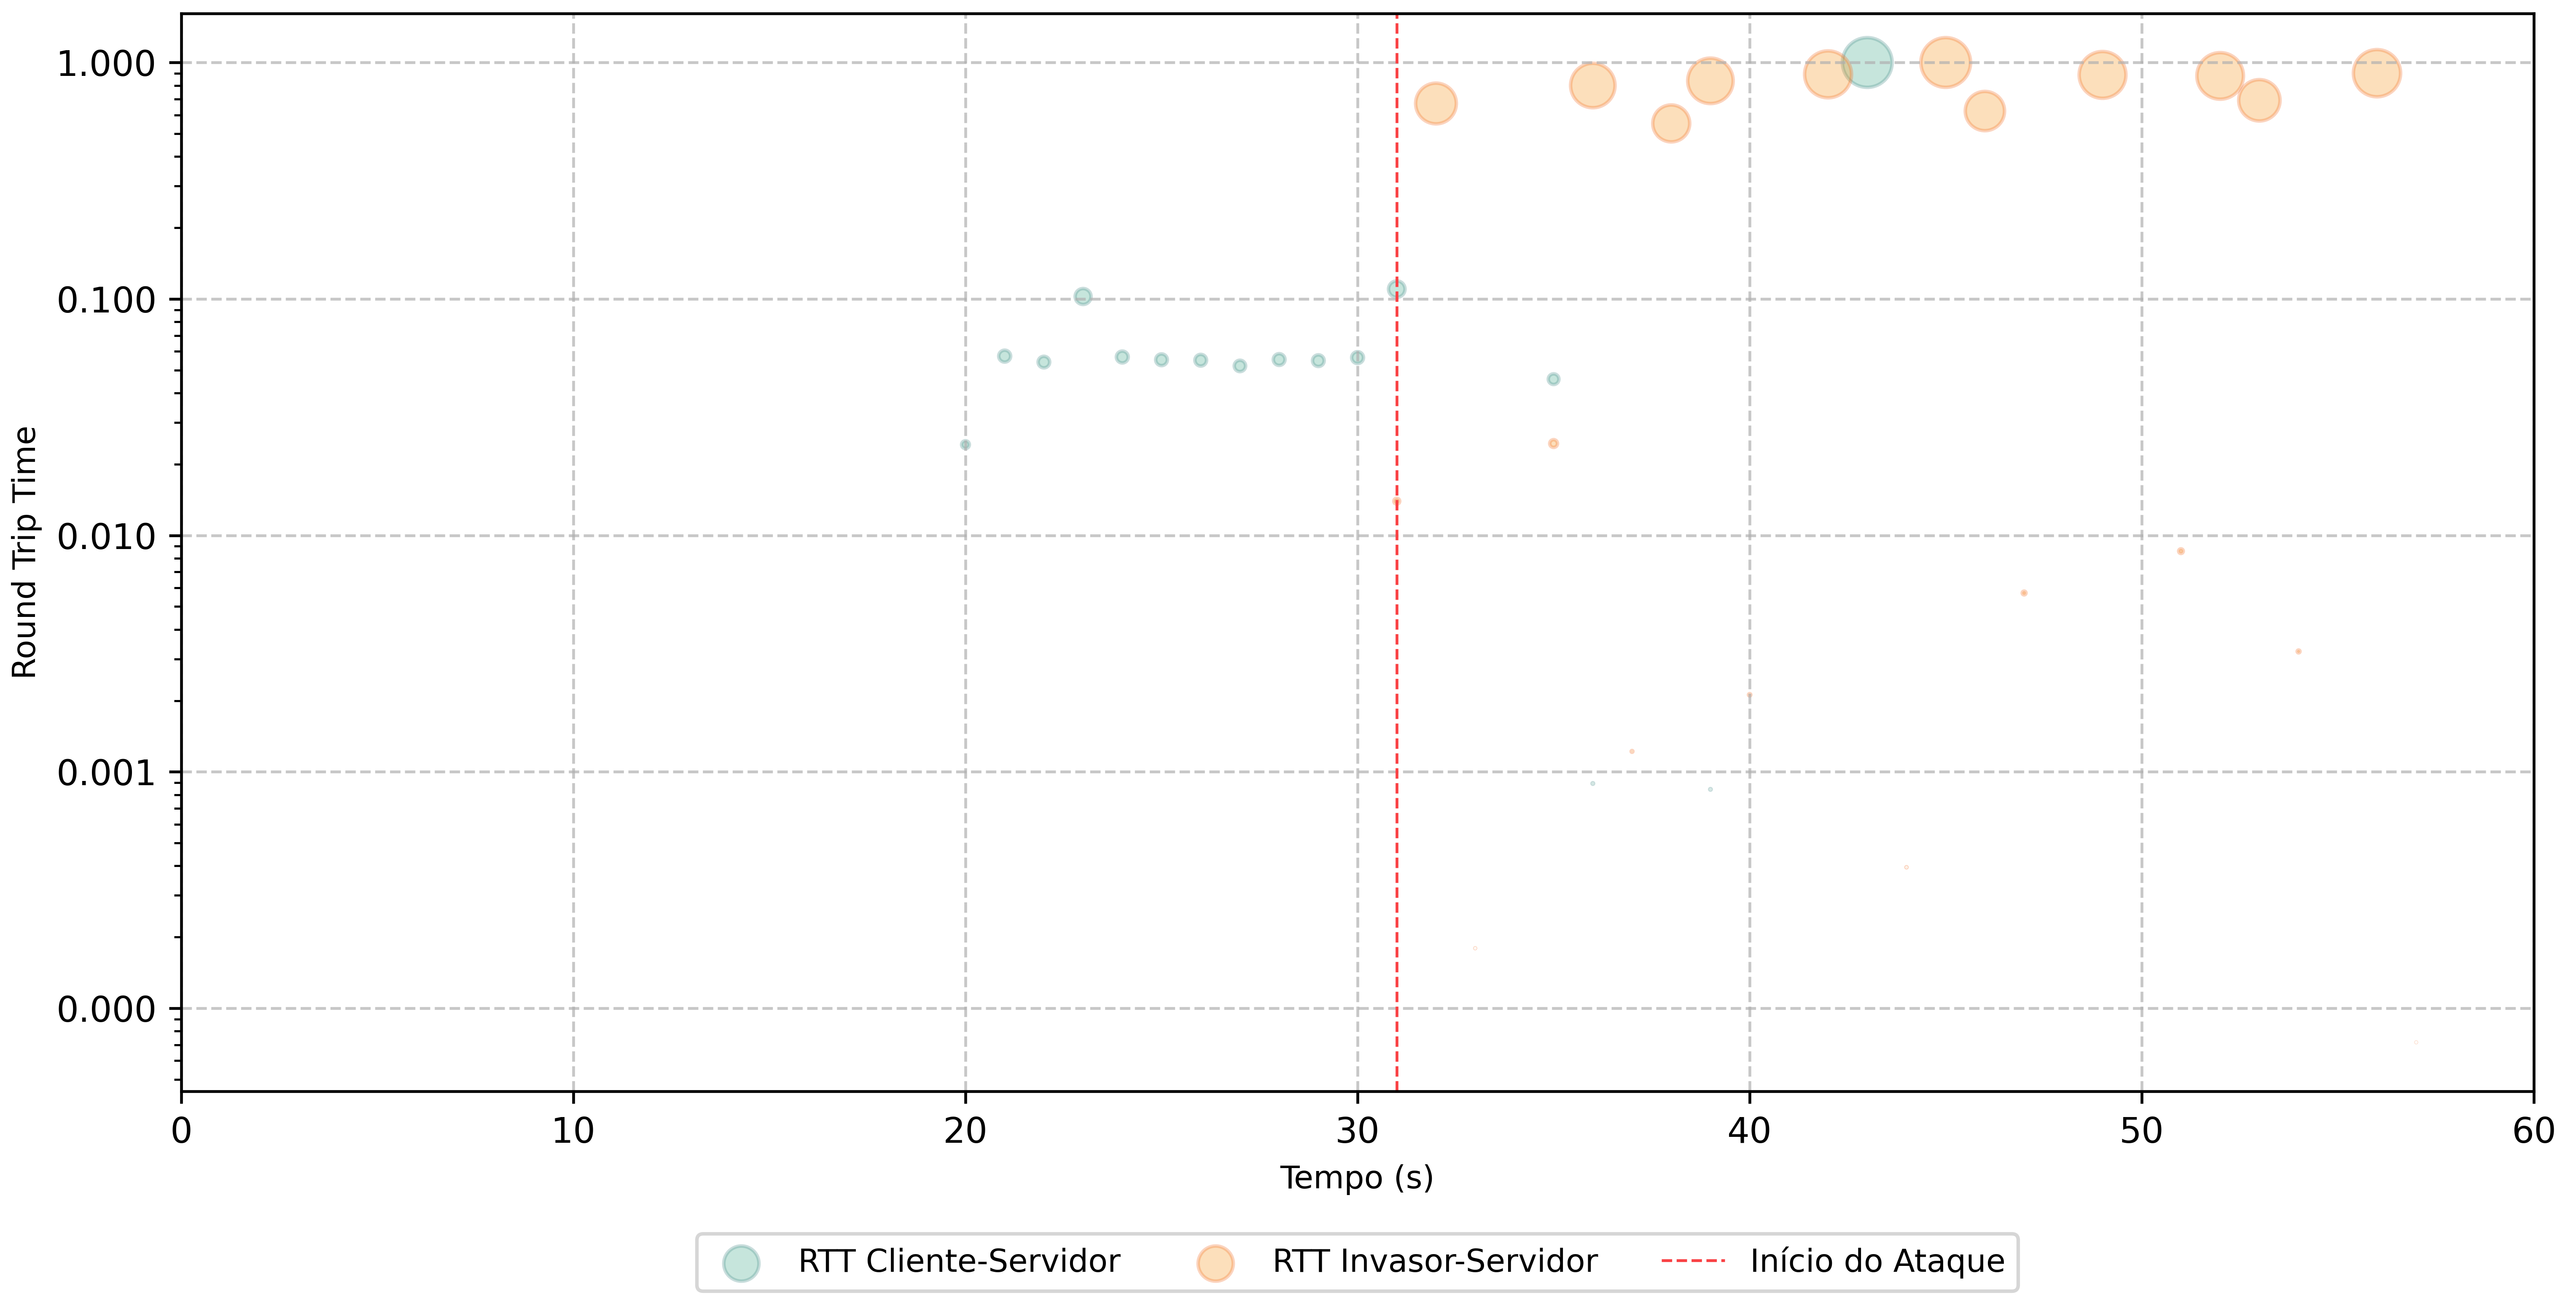
\includegraphics[width=1\textwidth, height=120pt]{USPSC-img/output/cropped/0-dos_function_call_null_deref-rtts.png}
    % \end{subfigure}%
\end{figure}

\begin{figure}[htbp!]
    \centering
    \caption{\label{fig:1-dos_function_call_null_deref}Gráficos do ataque de DoS pela chamada da função \textit{Dereference} nula - nível de segurança: `Sign'.}
    \begin{subfigure}[t]{0.5\textwidth}
        \centering
        \caption{\textit{Throughput}}
        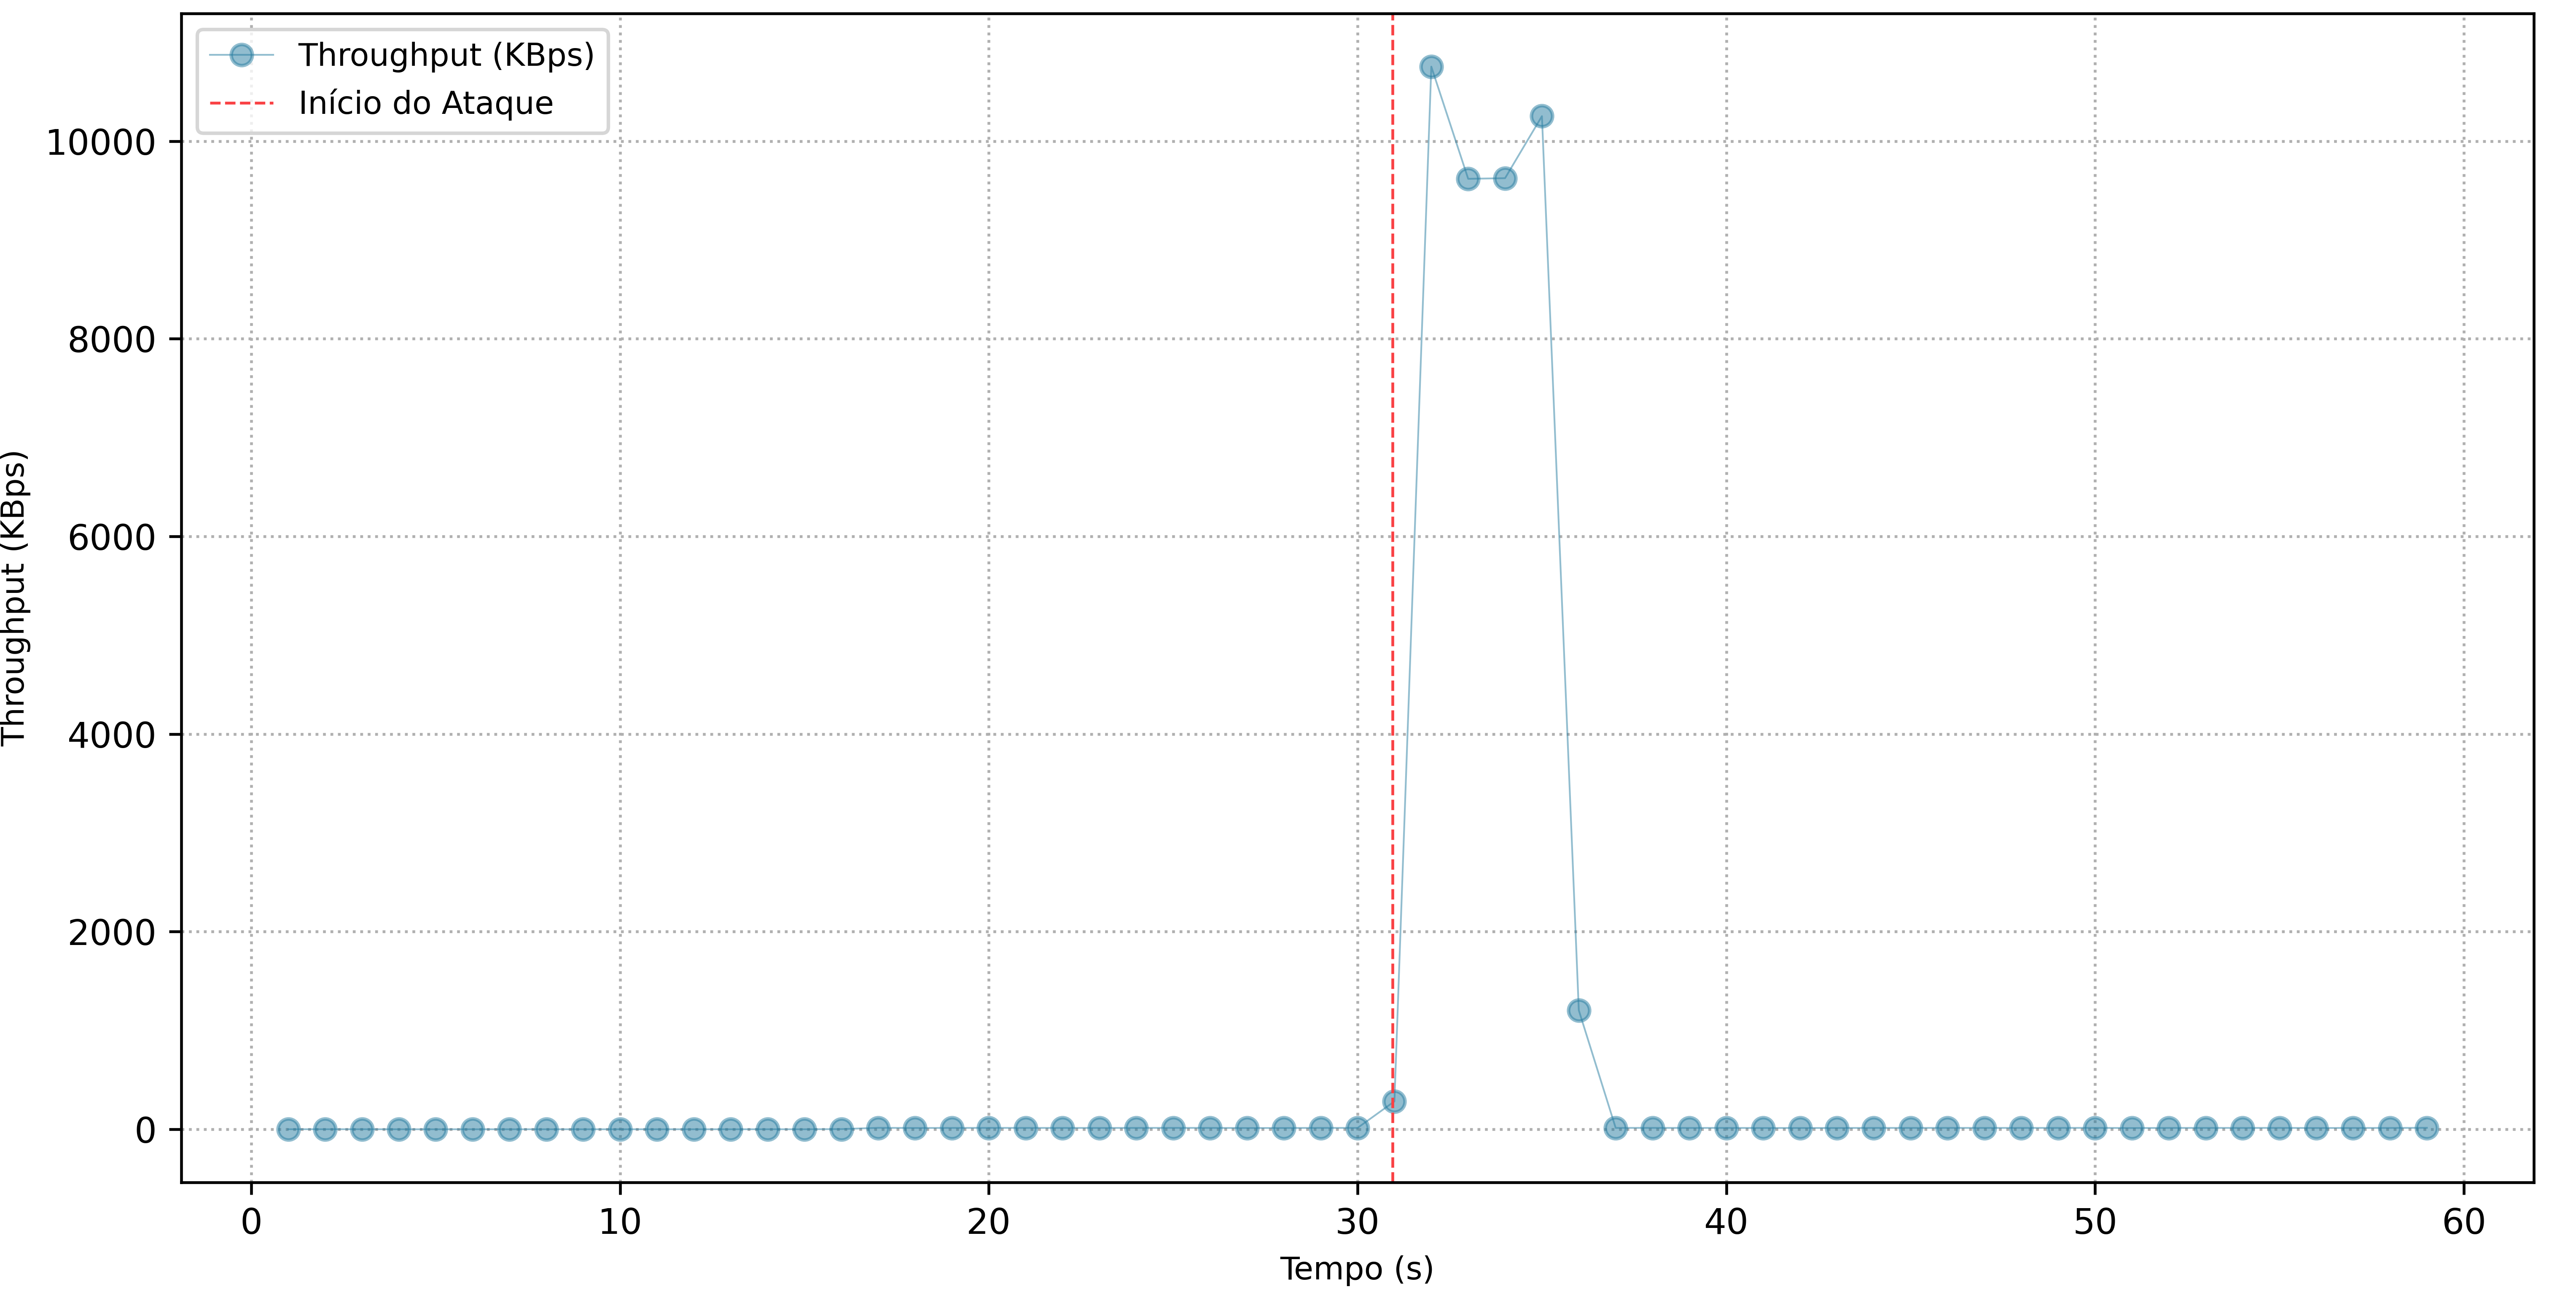
\includegraphics[width=1\textwidth, height=120pt]{USPSC-img/output/cropped/1-dos_function_call_null_deref-tput.png}
    \end{subfigure}%
    ~ 
    \begin{subfigure}[t]{0.5\textwidth}
        \centering
        \caption{Desempenho}
        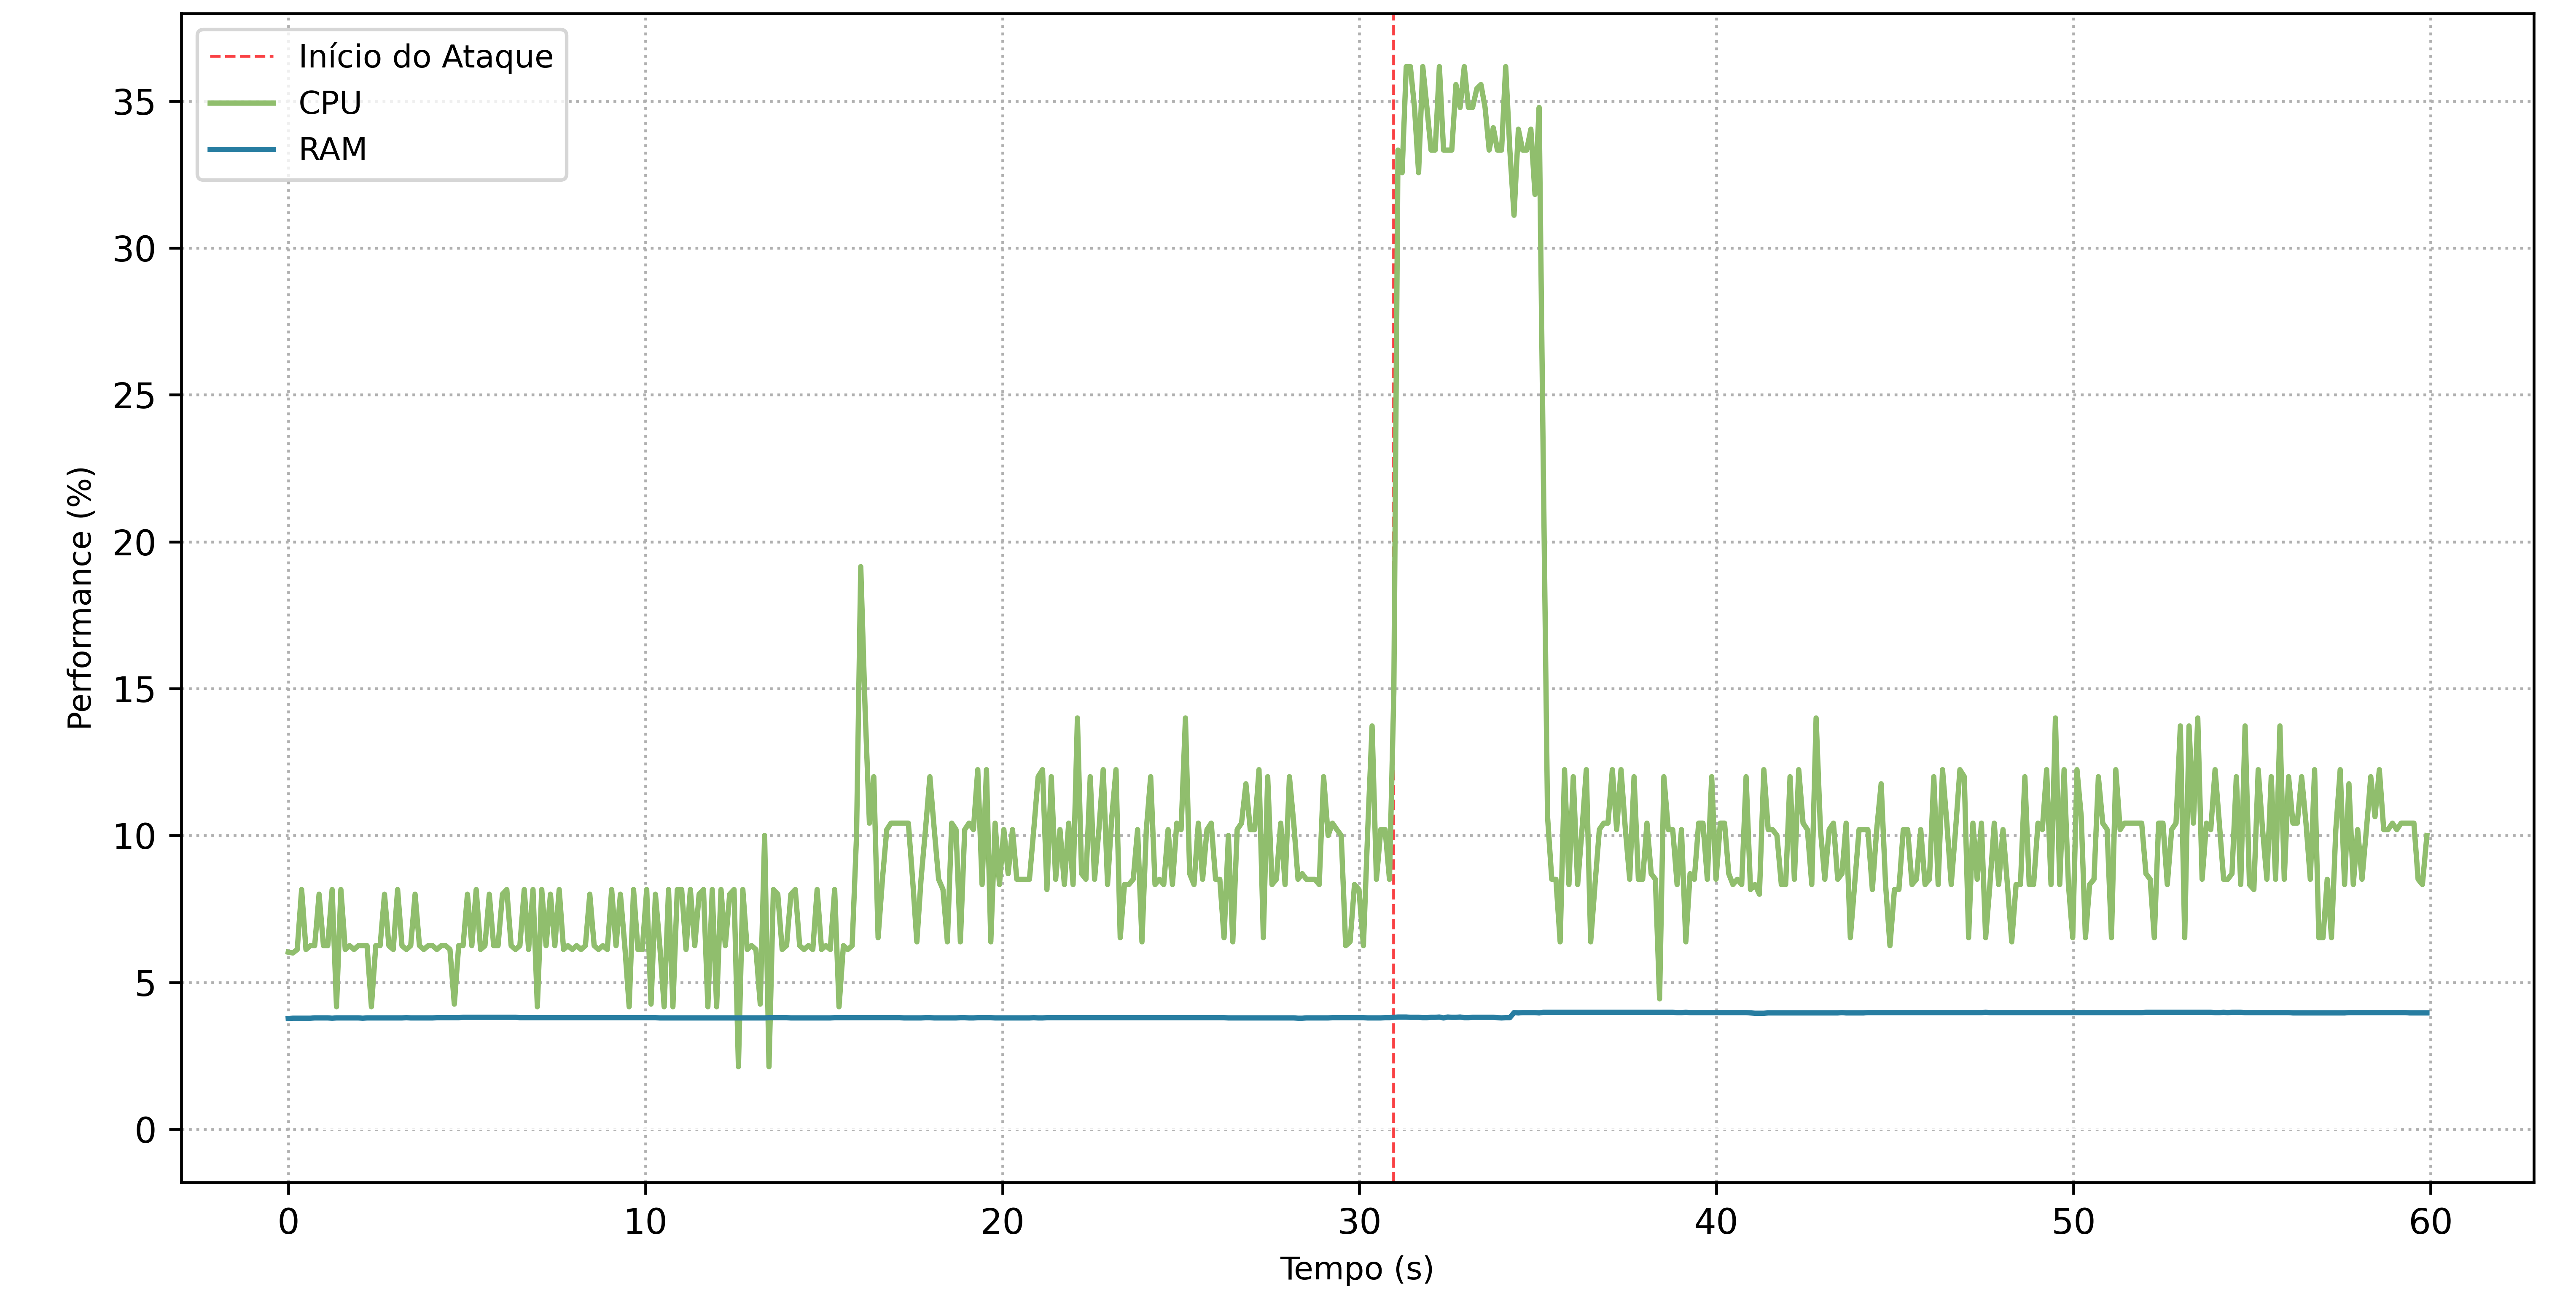
\includegraphics[width=1\textwidth, height=120pt]{USPSC-img/output/cropped/1-dos_function_call_null_deref-perf.png}
    \end{subfigure}%
    \\
    \begin{subfigure}[t]{0.5\textwidth}
        \centering
        \caption{Pacotes OPC UA}
        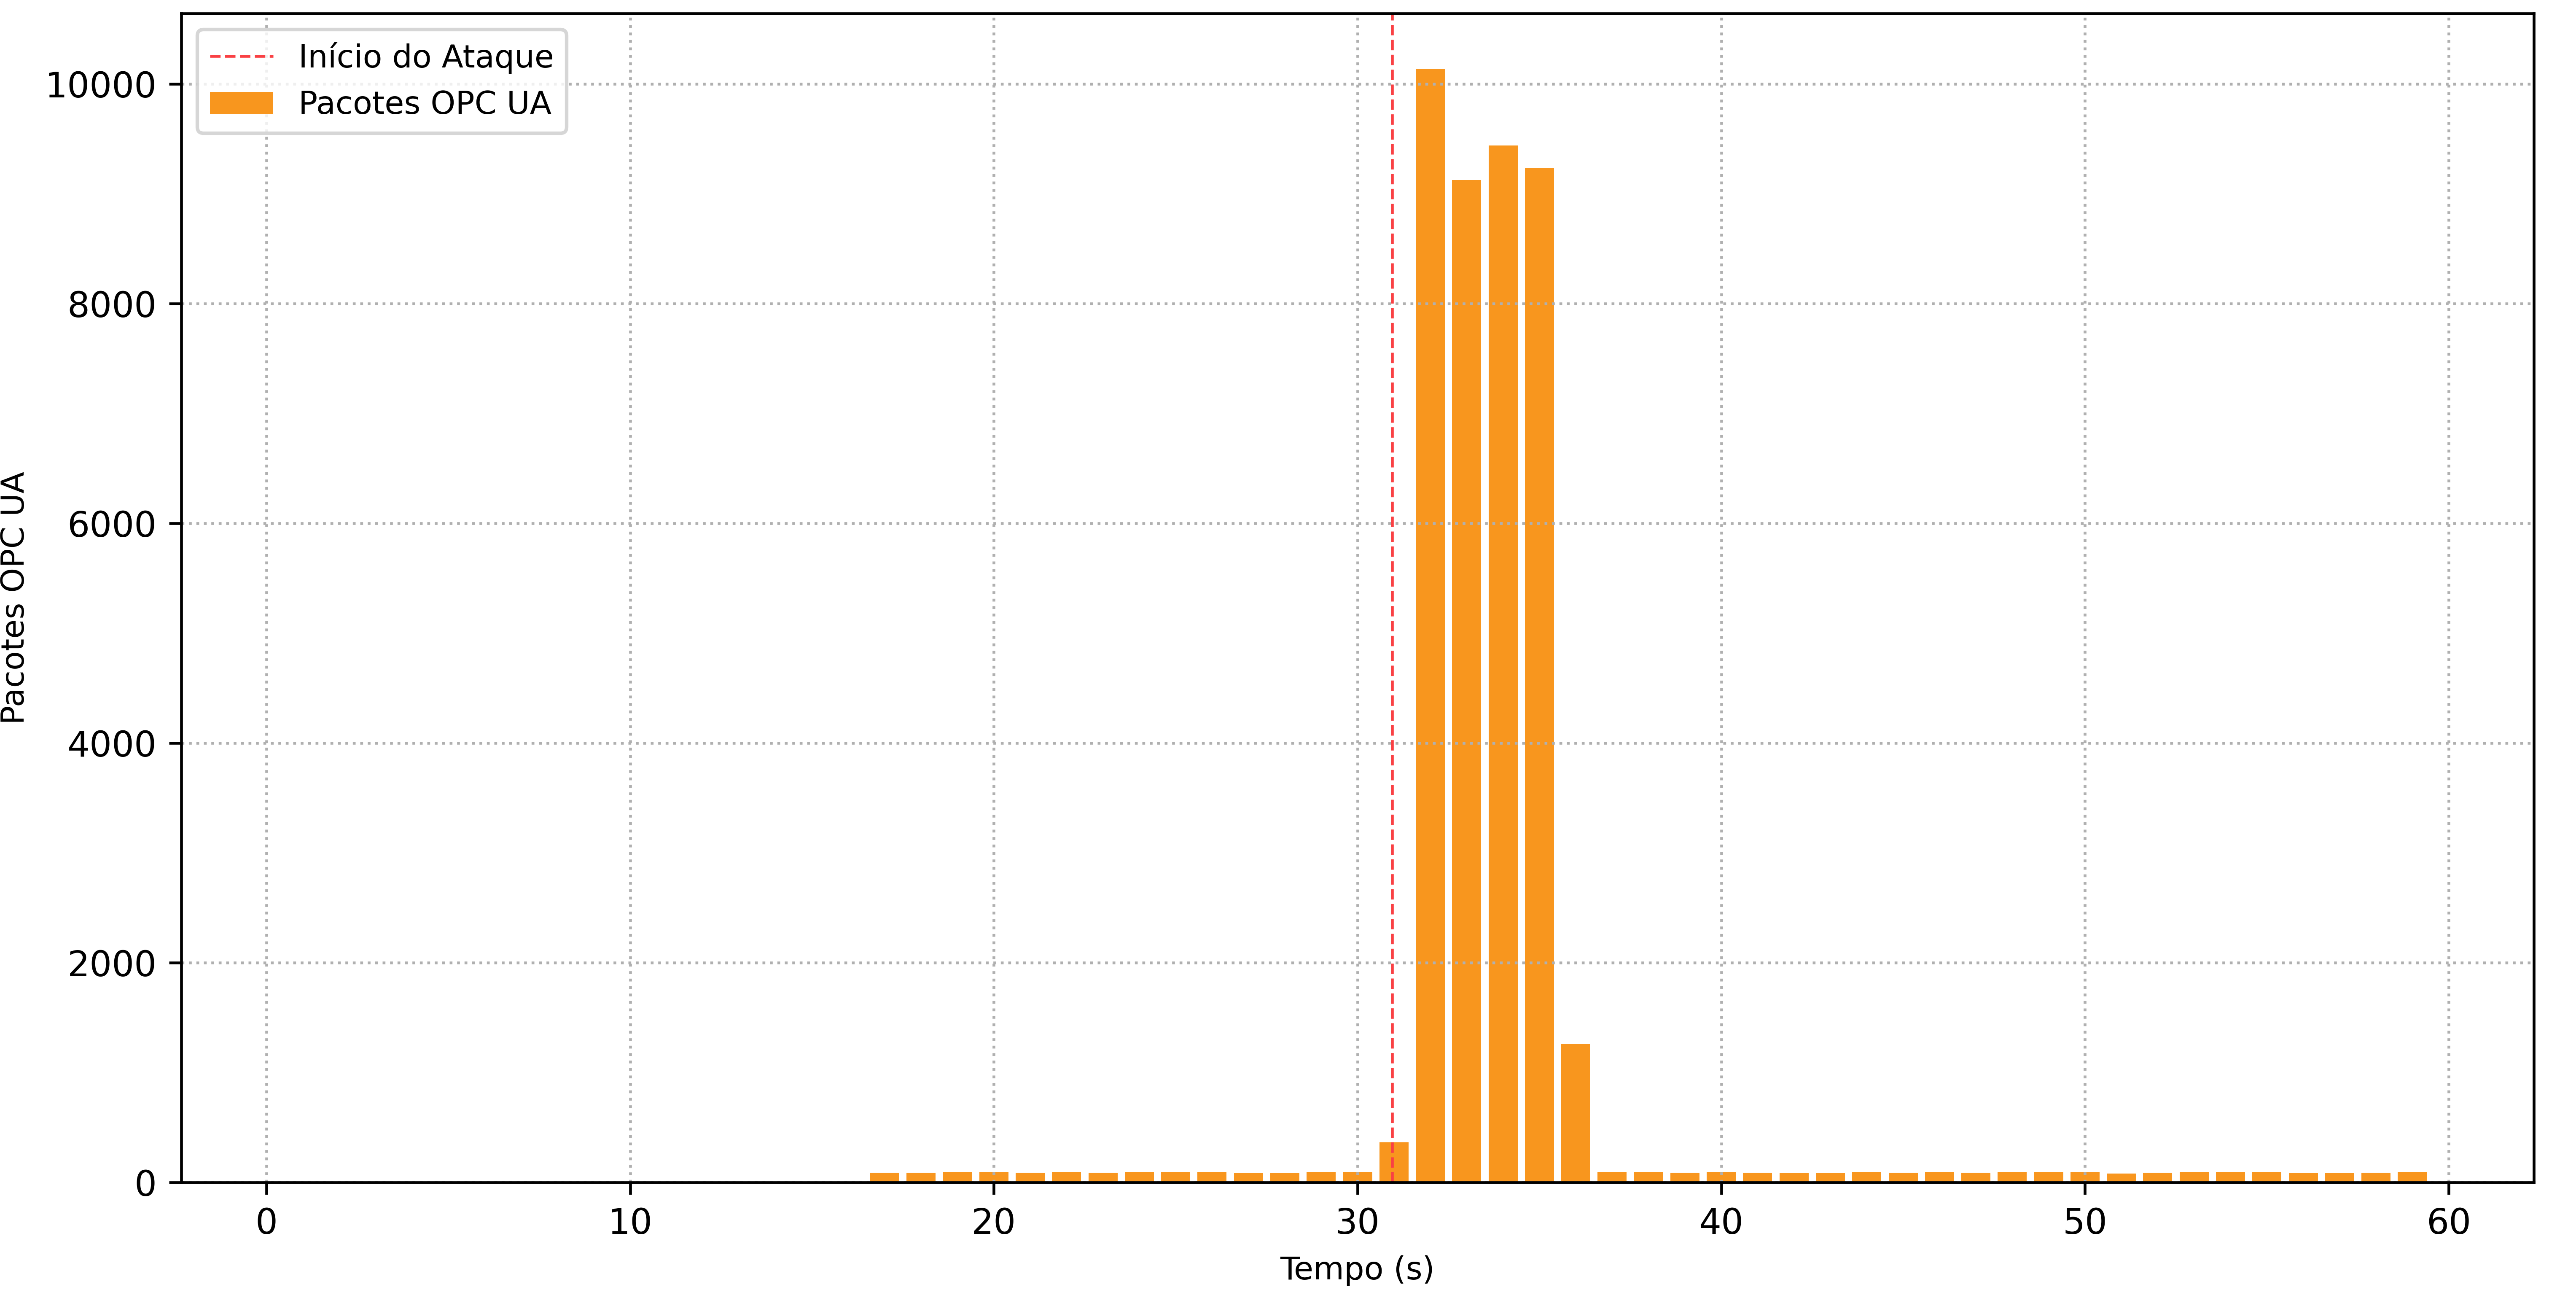
\includegraphics[width=1\textwidth, height=120pt]{USPSC-img/output/cropped/1-dos_function_call_null_deref-pack.png}
    \end{subfigure}%
    ~
    \begin{subfigure}[t]{0.5\textwidth}
        \centering
        \caption{RTT por pacote}
        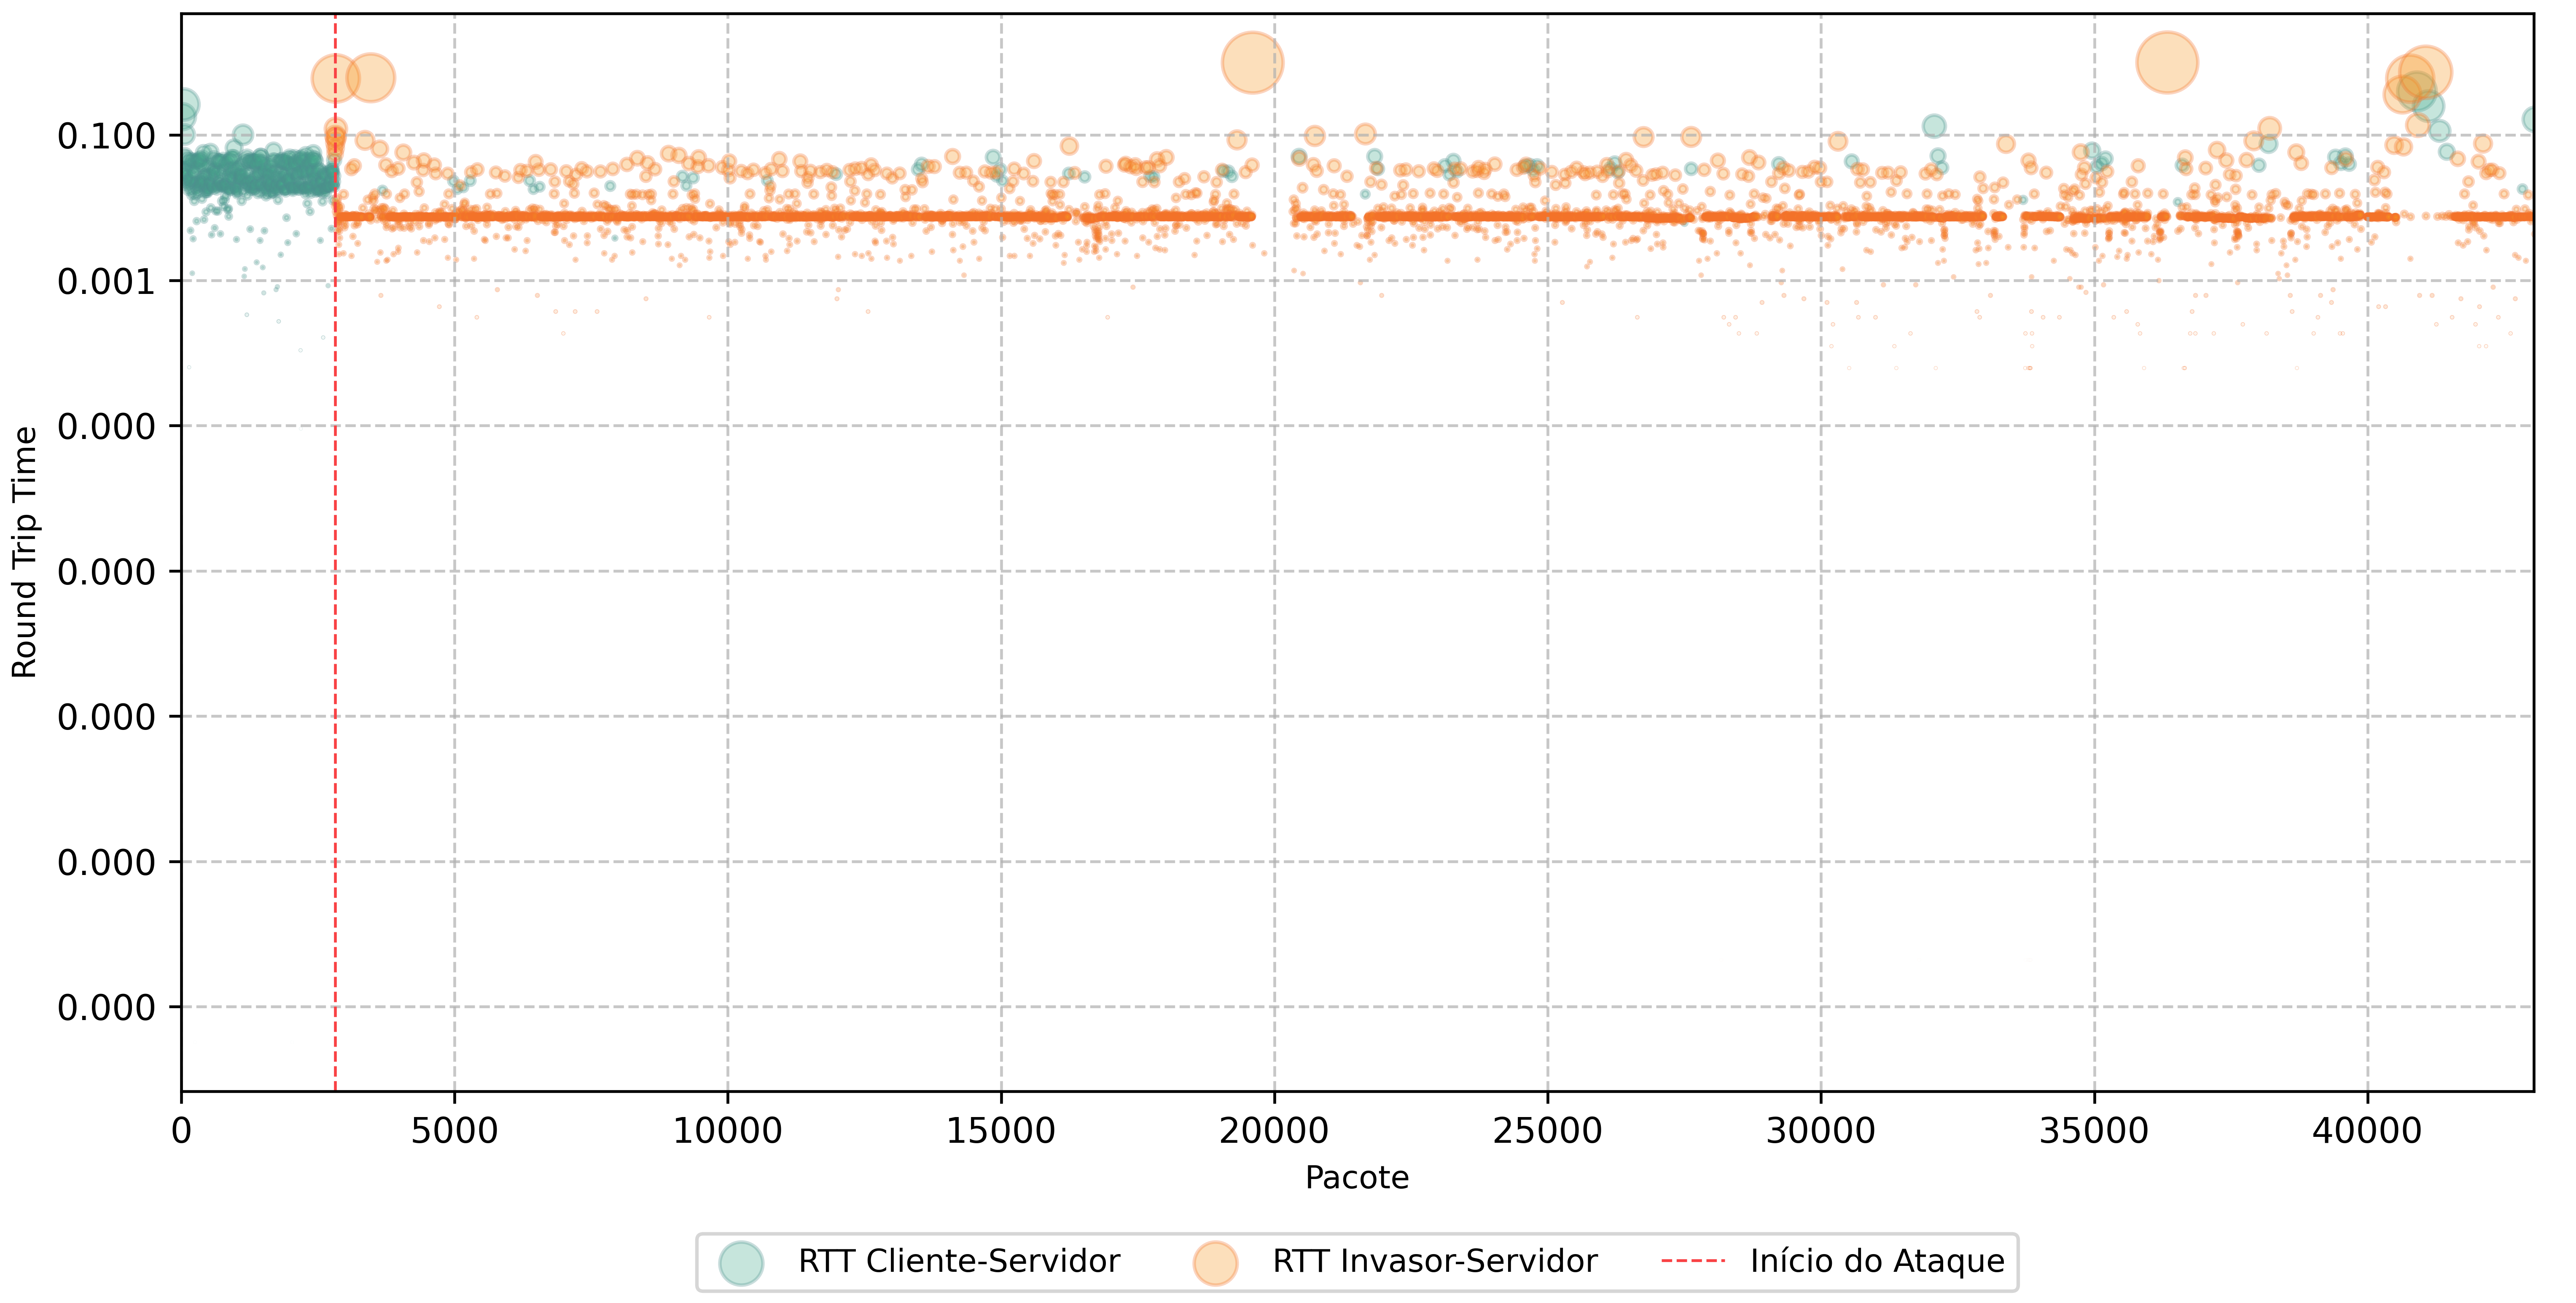
\includegraphics[width=1\textwidth, height=120pt]{USPSC-img/output/cropped/1-dos_function_call_null_deref-rttp.png}
    \end{subfigure}%
    % ~
    % \begin{subfigure}[t]{0.5\textwidth}
    %     \centering
    %     \caption{RTT por segundos}
    %     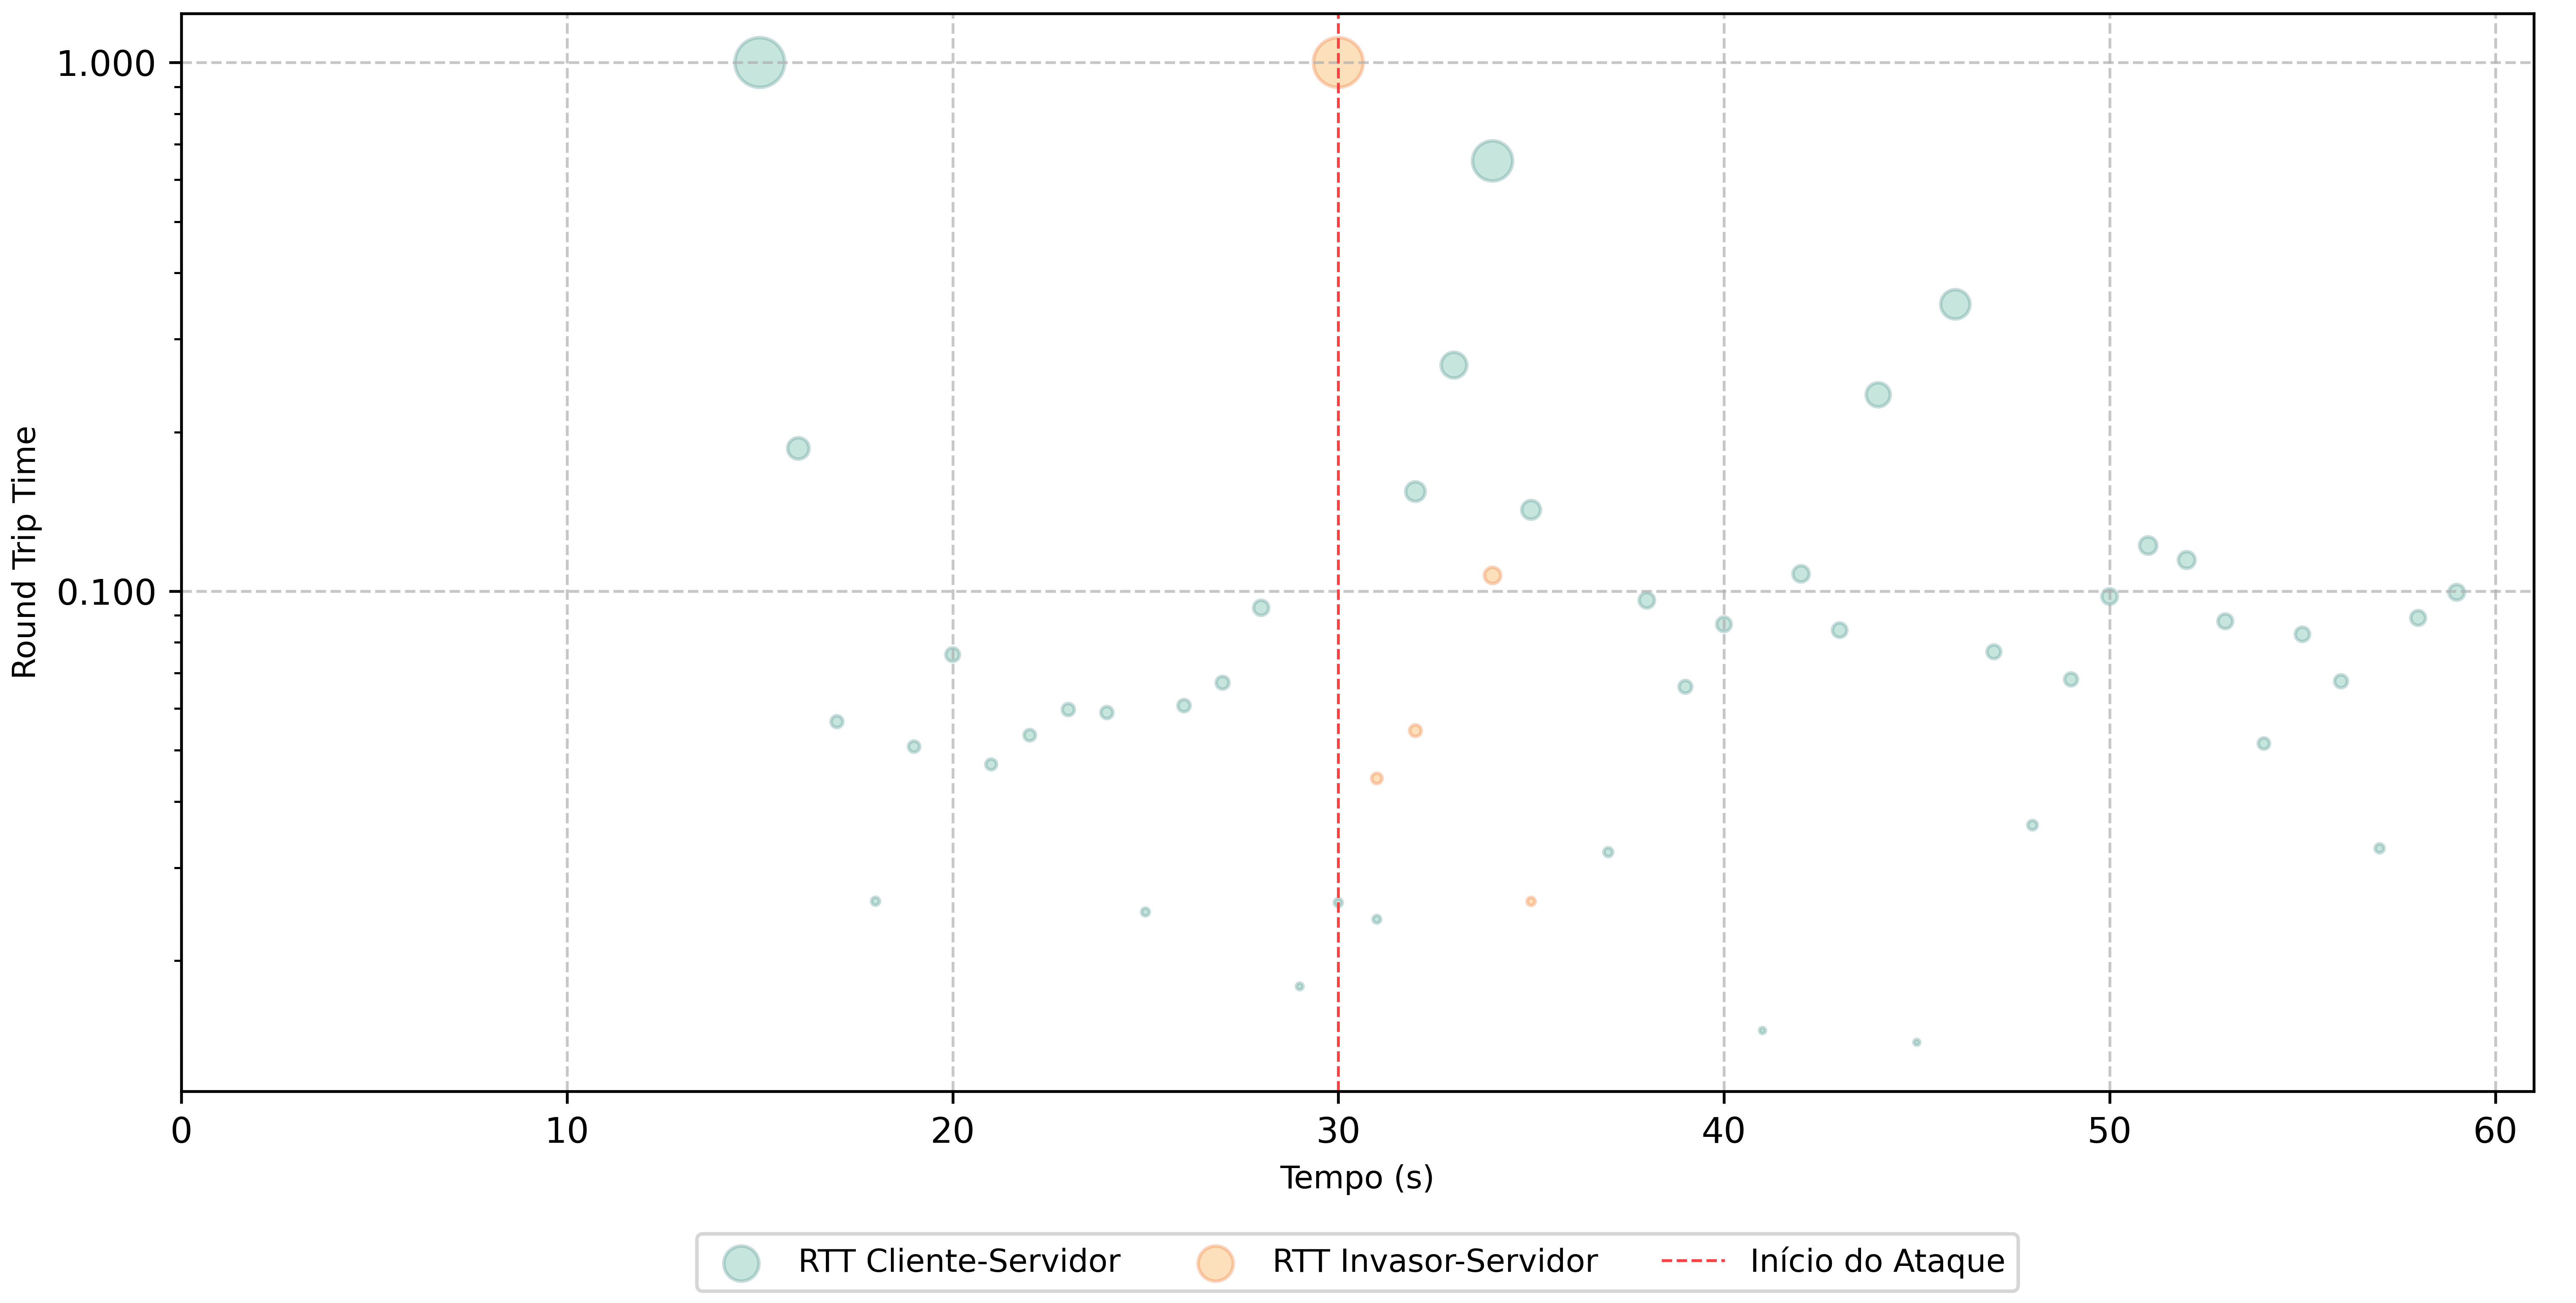
\includegraphics[width=1\textwidth, height=120pt]{USPSC-img/output/cropped/1-dos_function_call_null_deref-rtts.png}
    % \end{subfigure}%
\end{figure}

\begin{figure}[htbp!]
    \centering
    \caption{\label{fig:2-dos_function_call_null_deref}Gráficos do ataque de DoS pela chamada da função \textit{Dereference} nula - nível de segurança: `Sign \& Encrypt'.}
    \begin{subfigure}[t]{0.5\textwidth}
        \centering
        \caption{\textit{Throughput}}
        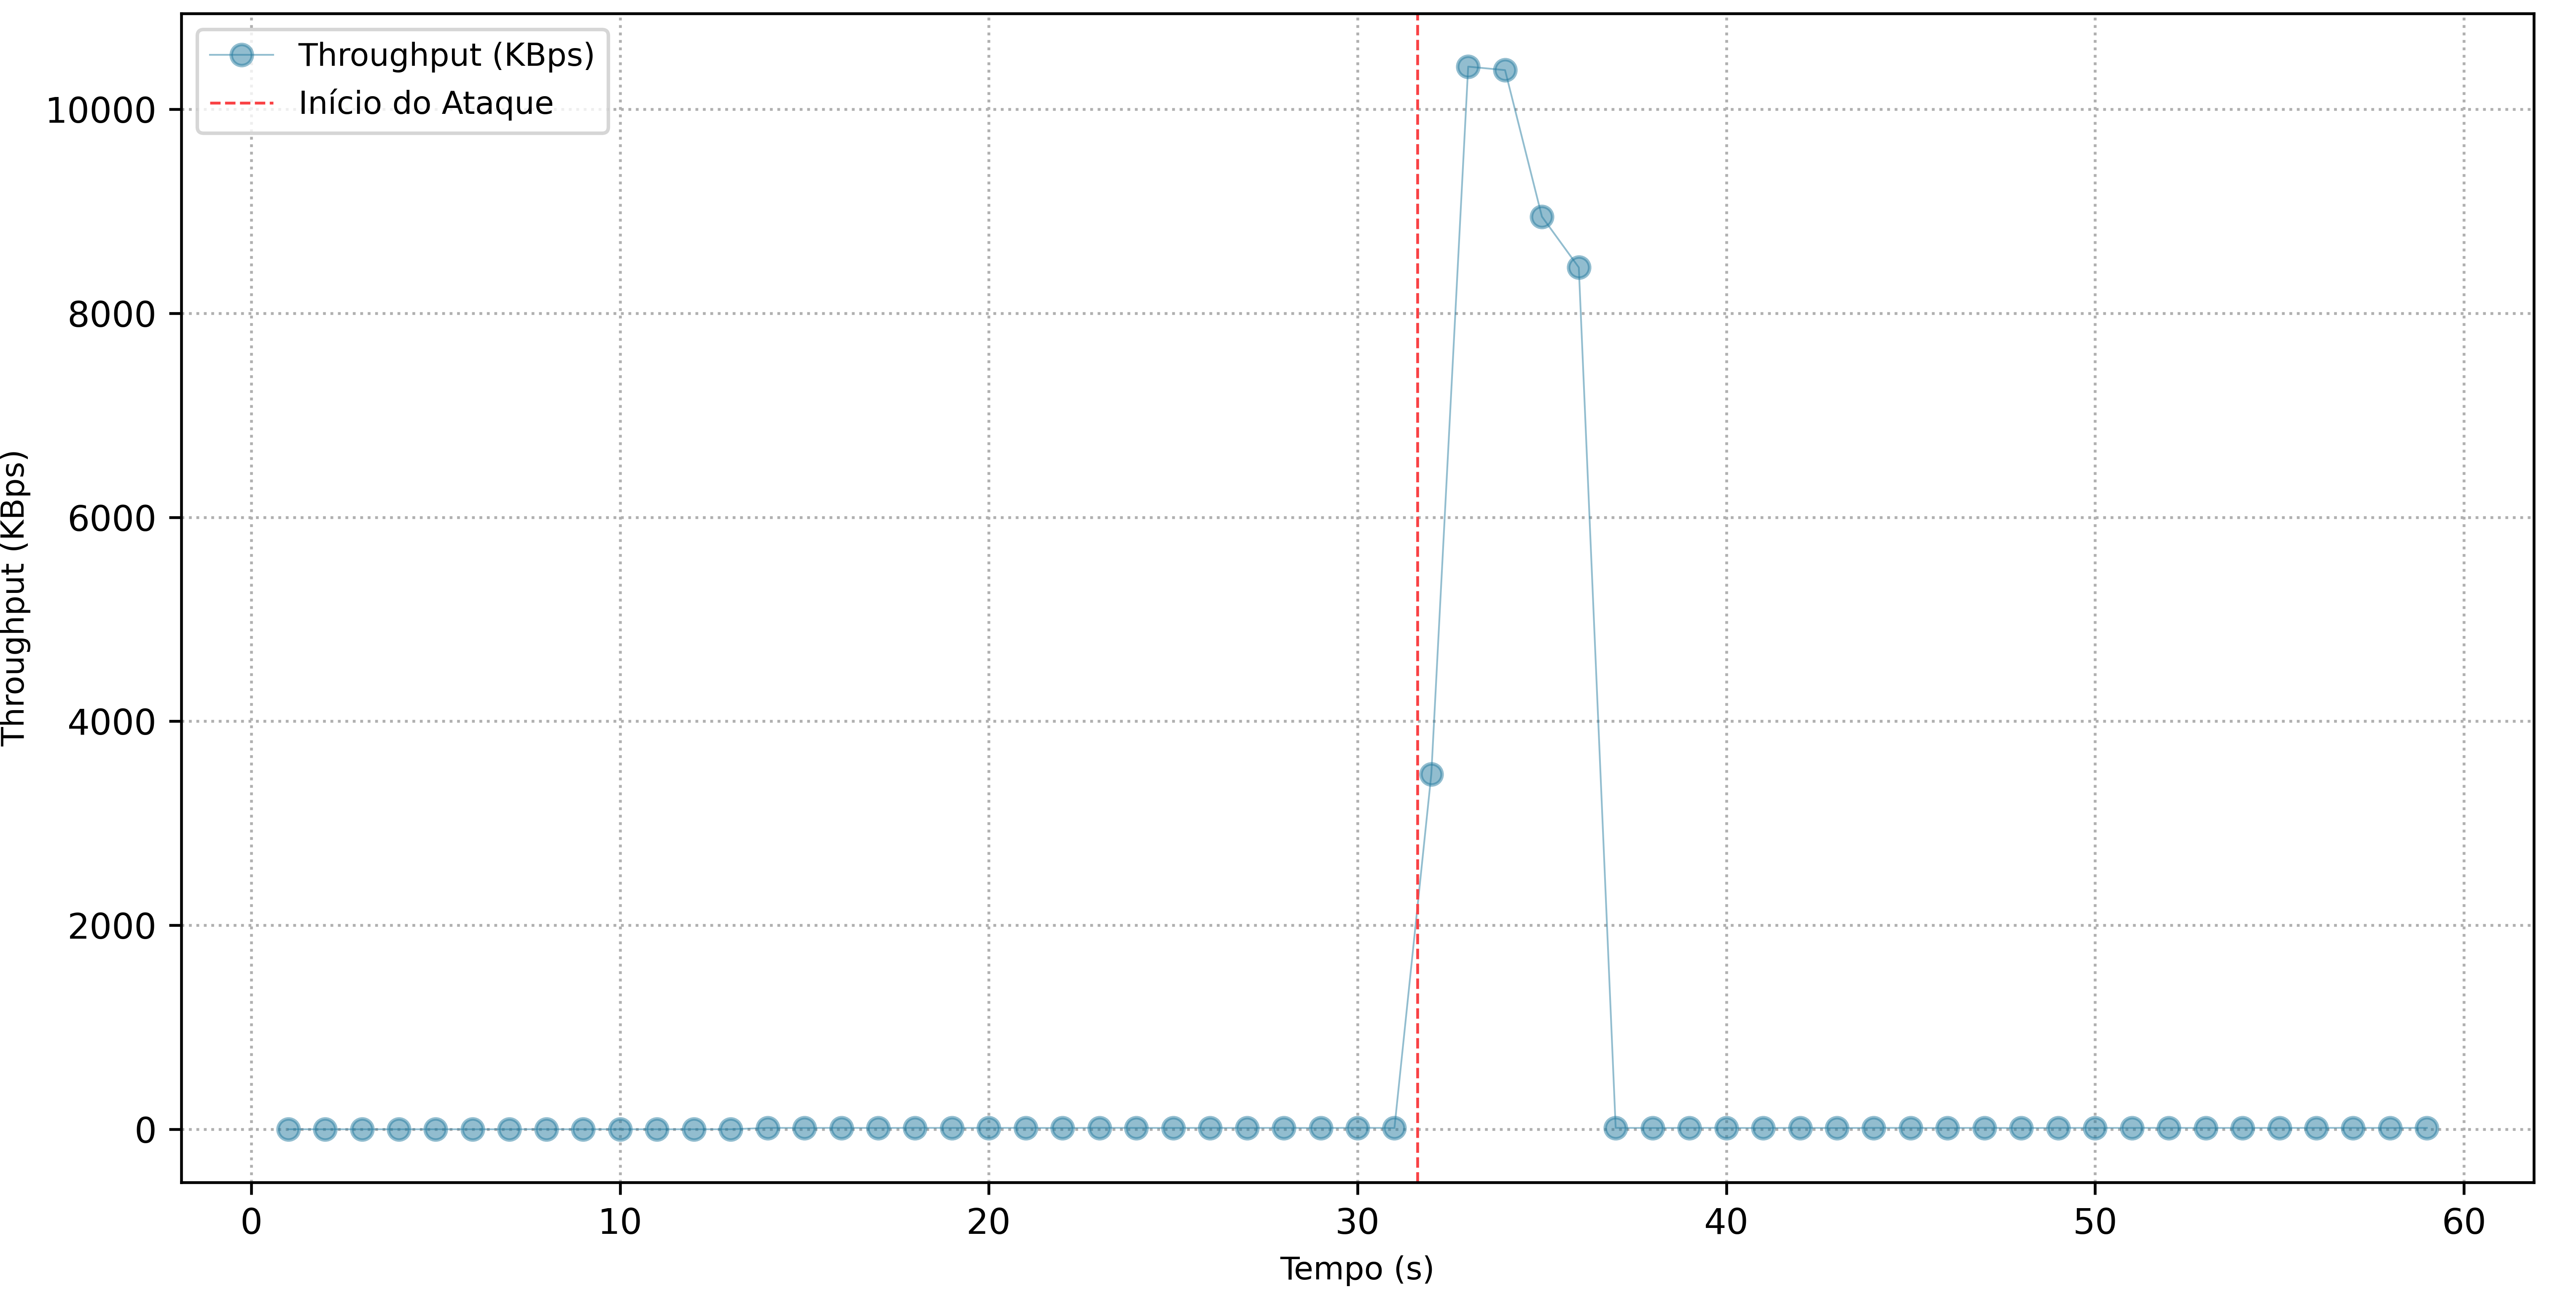
\includegraphics[width=1\textwidth, height=120pt]{USPSC-img/output/cropped/2-dos_function_call_null_deref-tput.png}
    \end{subfigure}%
    ~ 
    \begin{subfigure}[t]{0.5\textwidth}
        \centering
        \caption{Desempenho}
        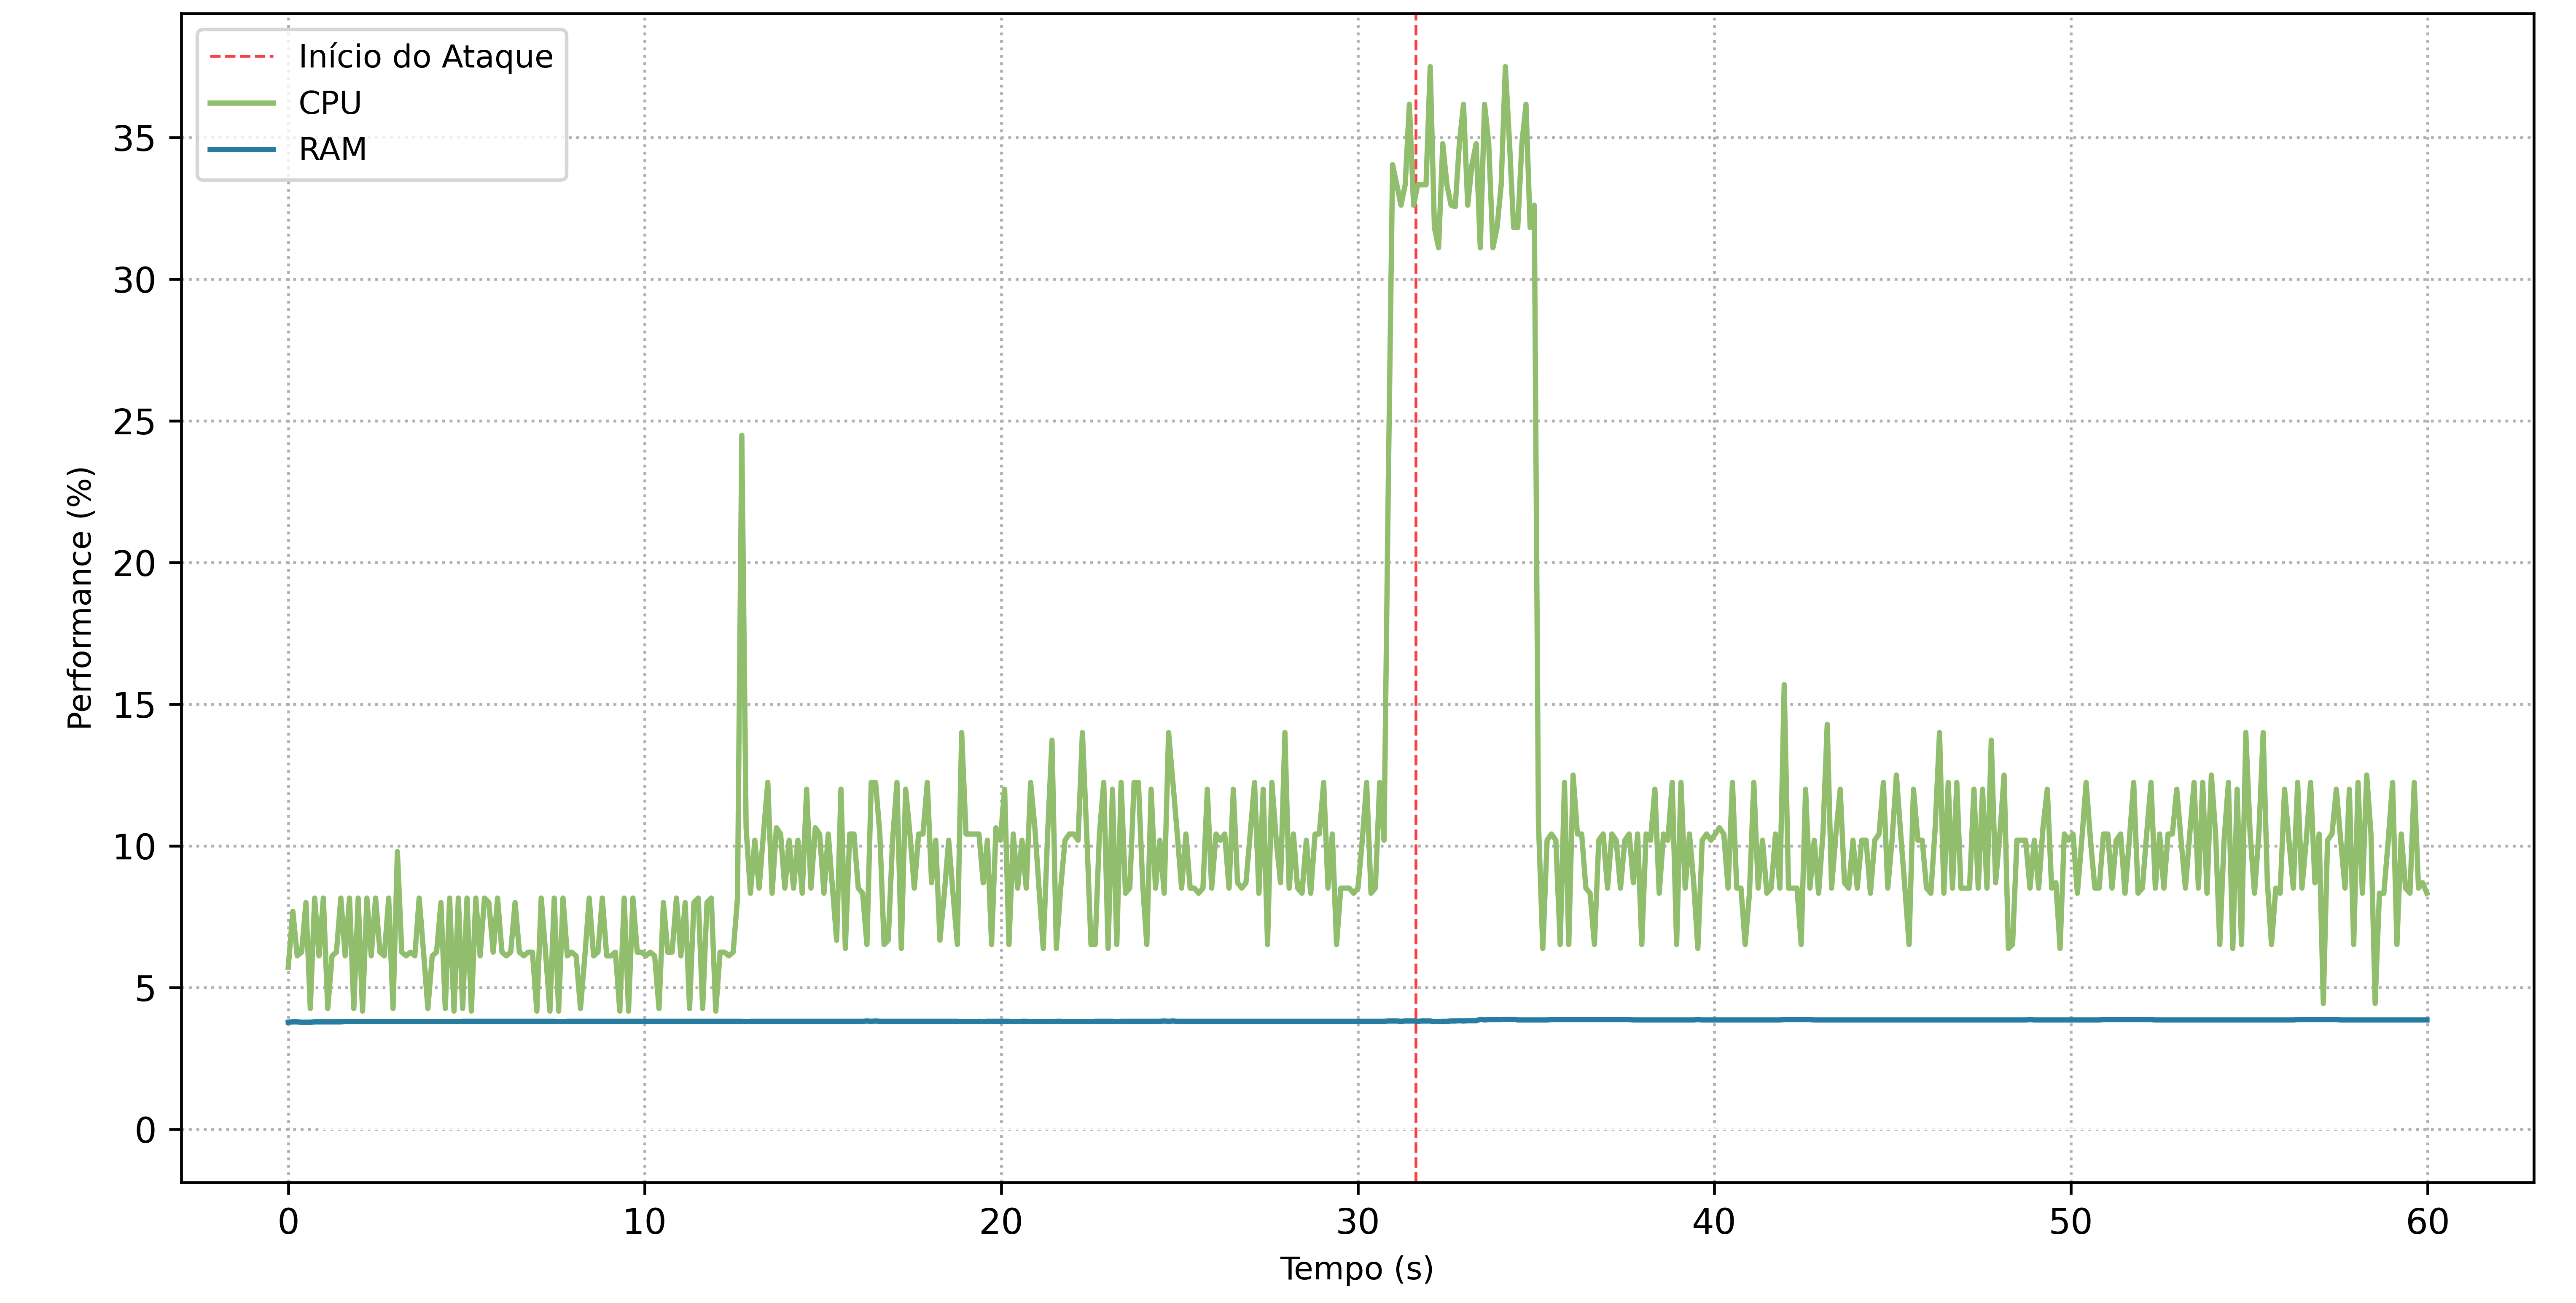
\includegraphics[width=1\textwidth, height=120pt]{USPSC-img/output/cropped/2-dos_function_call_null_deref-perf.png}
    \end{subfigure}%
    \\
    \begin{subfigure}[t]{0.5\textwidth}
        \centering
        \caption{Pacotes OPC UA}
        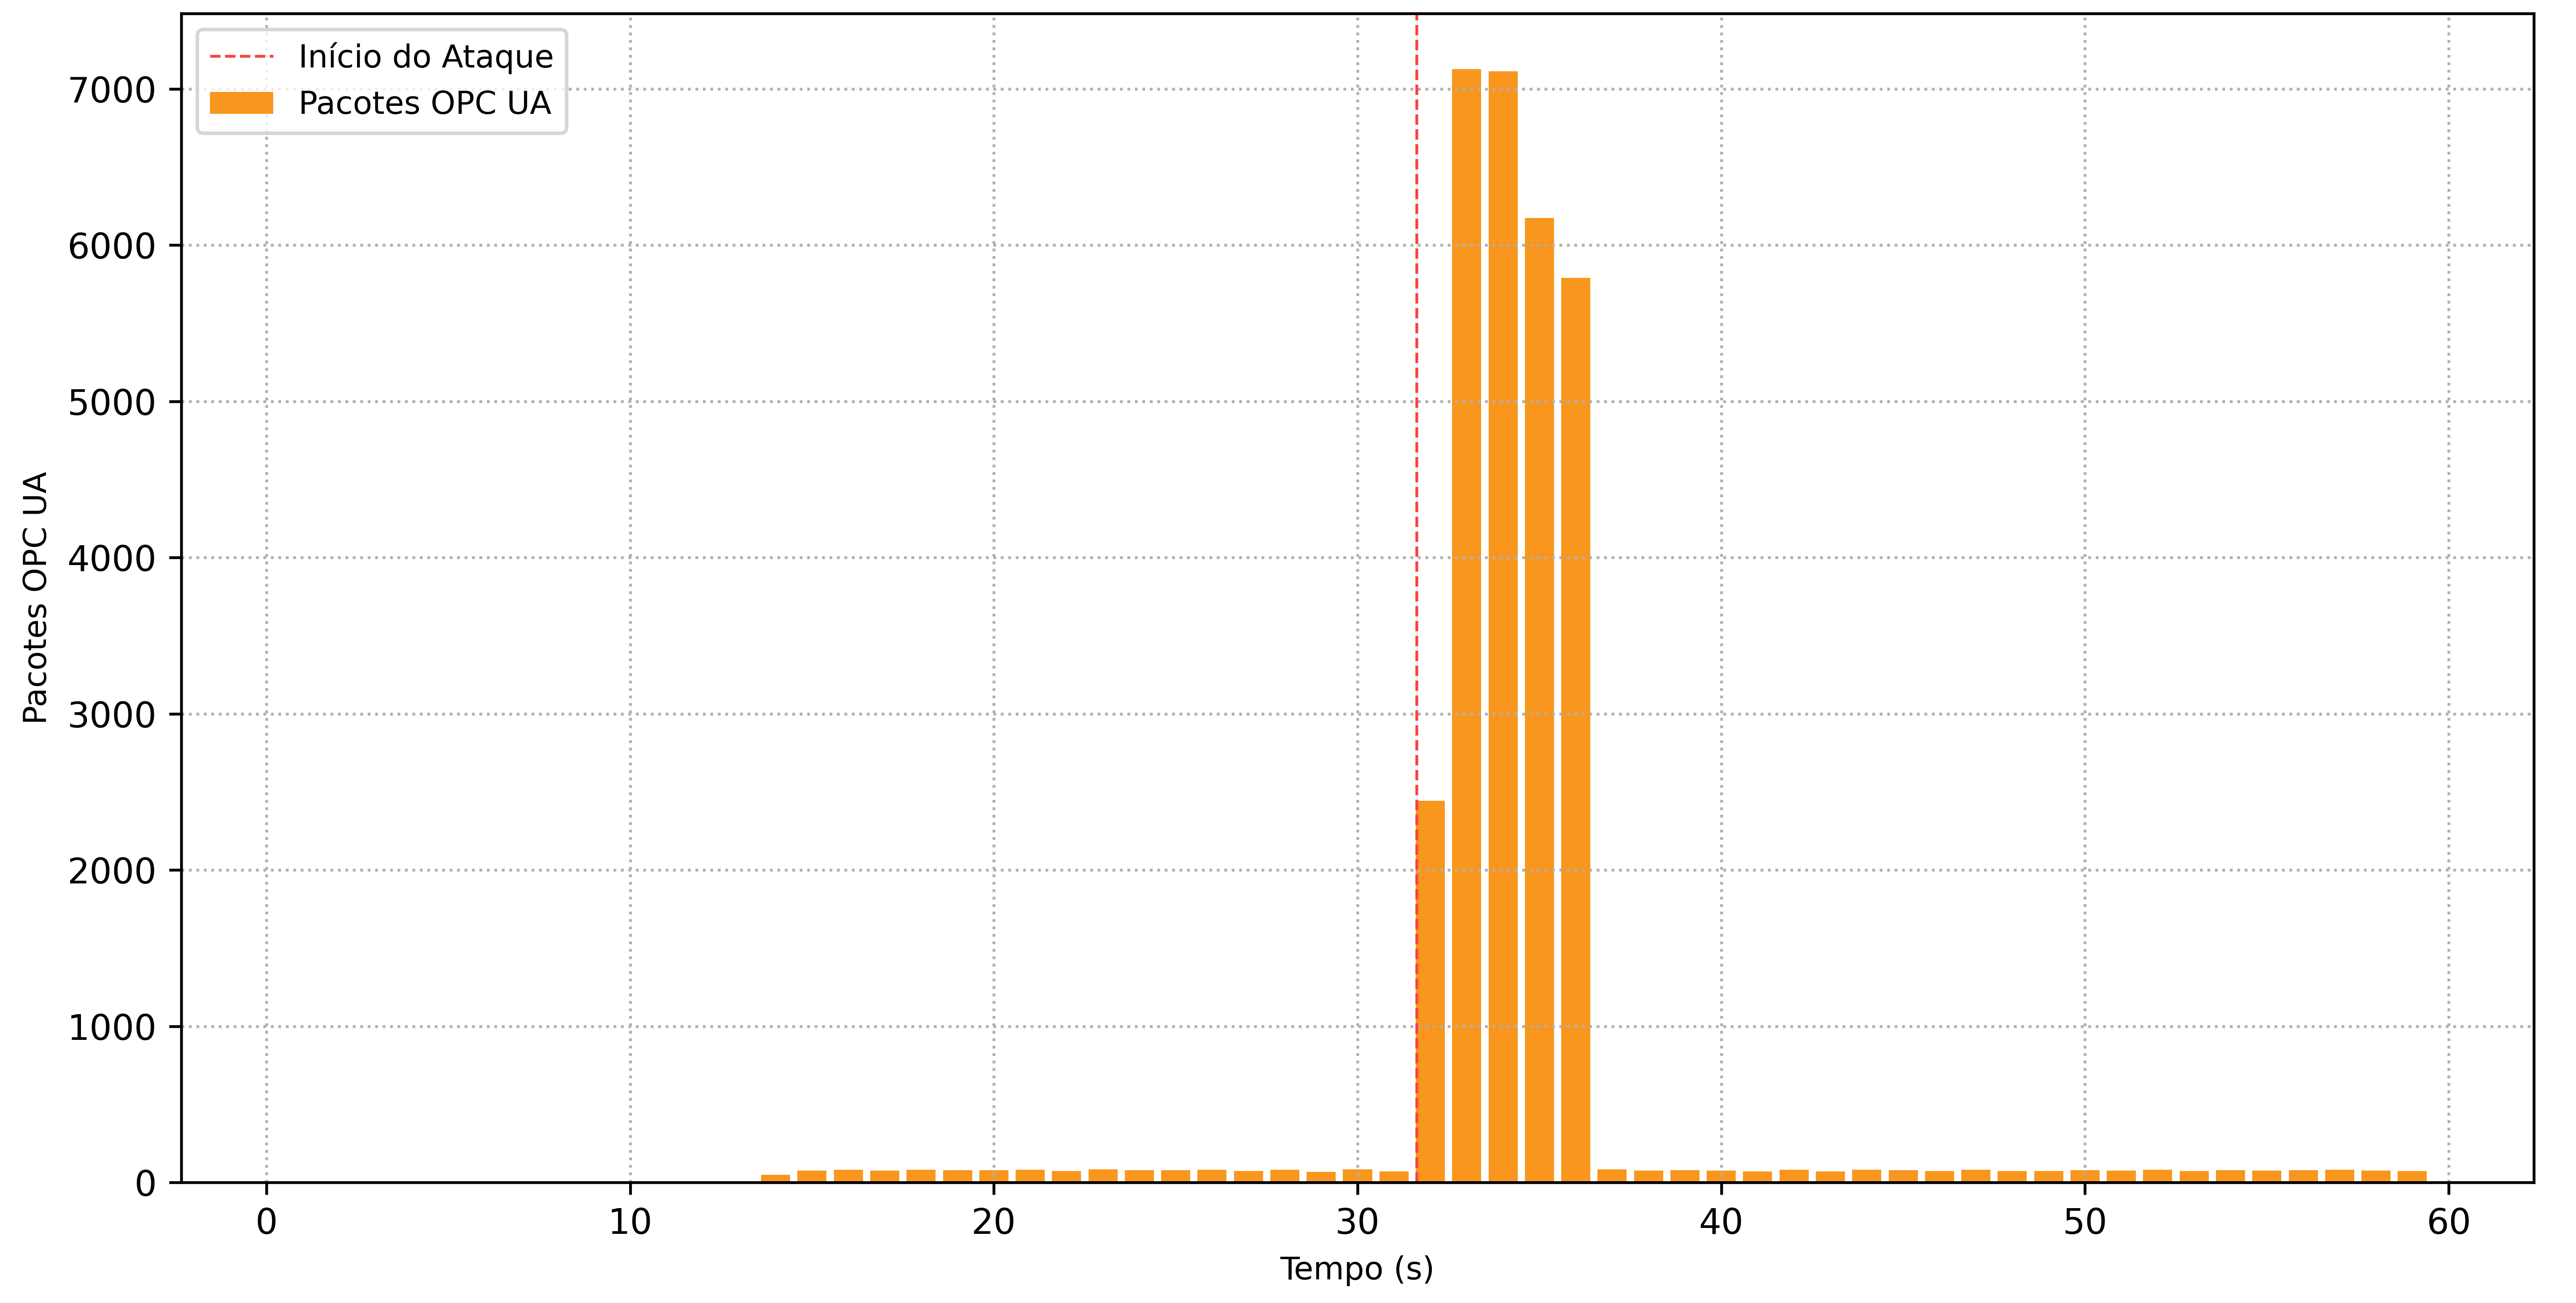
\includegraphics[width=1\textwidth, height=120pt]{USPSC-img/output/cropped/2-dos_function_call_null_deref-pack.png}
    \end{subfigure}%
    ~
    \begin{subfigure}[t]{0.5\textwidth}
        \centering
        \caption{RTT por pacote}
        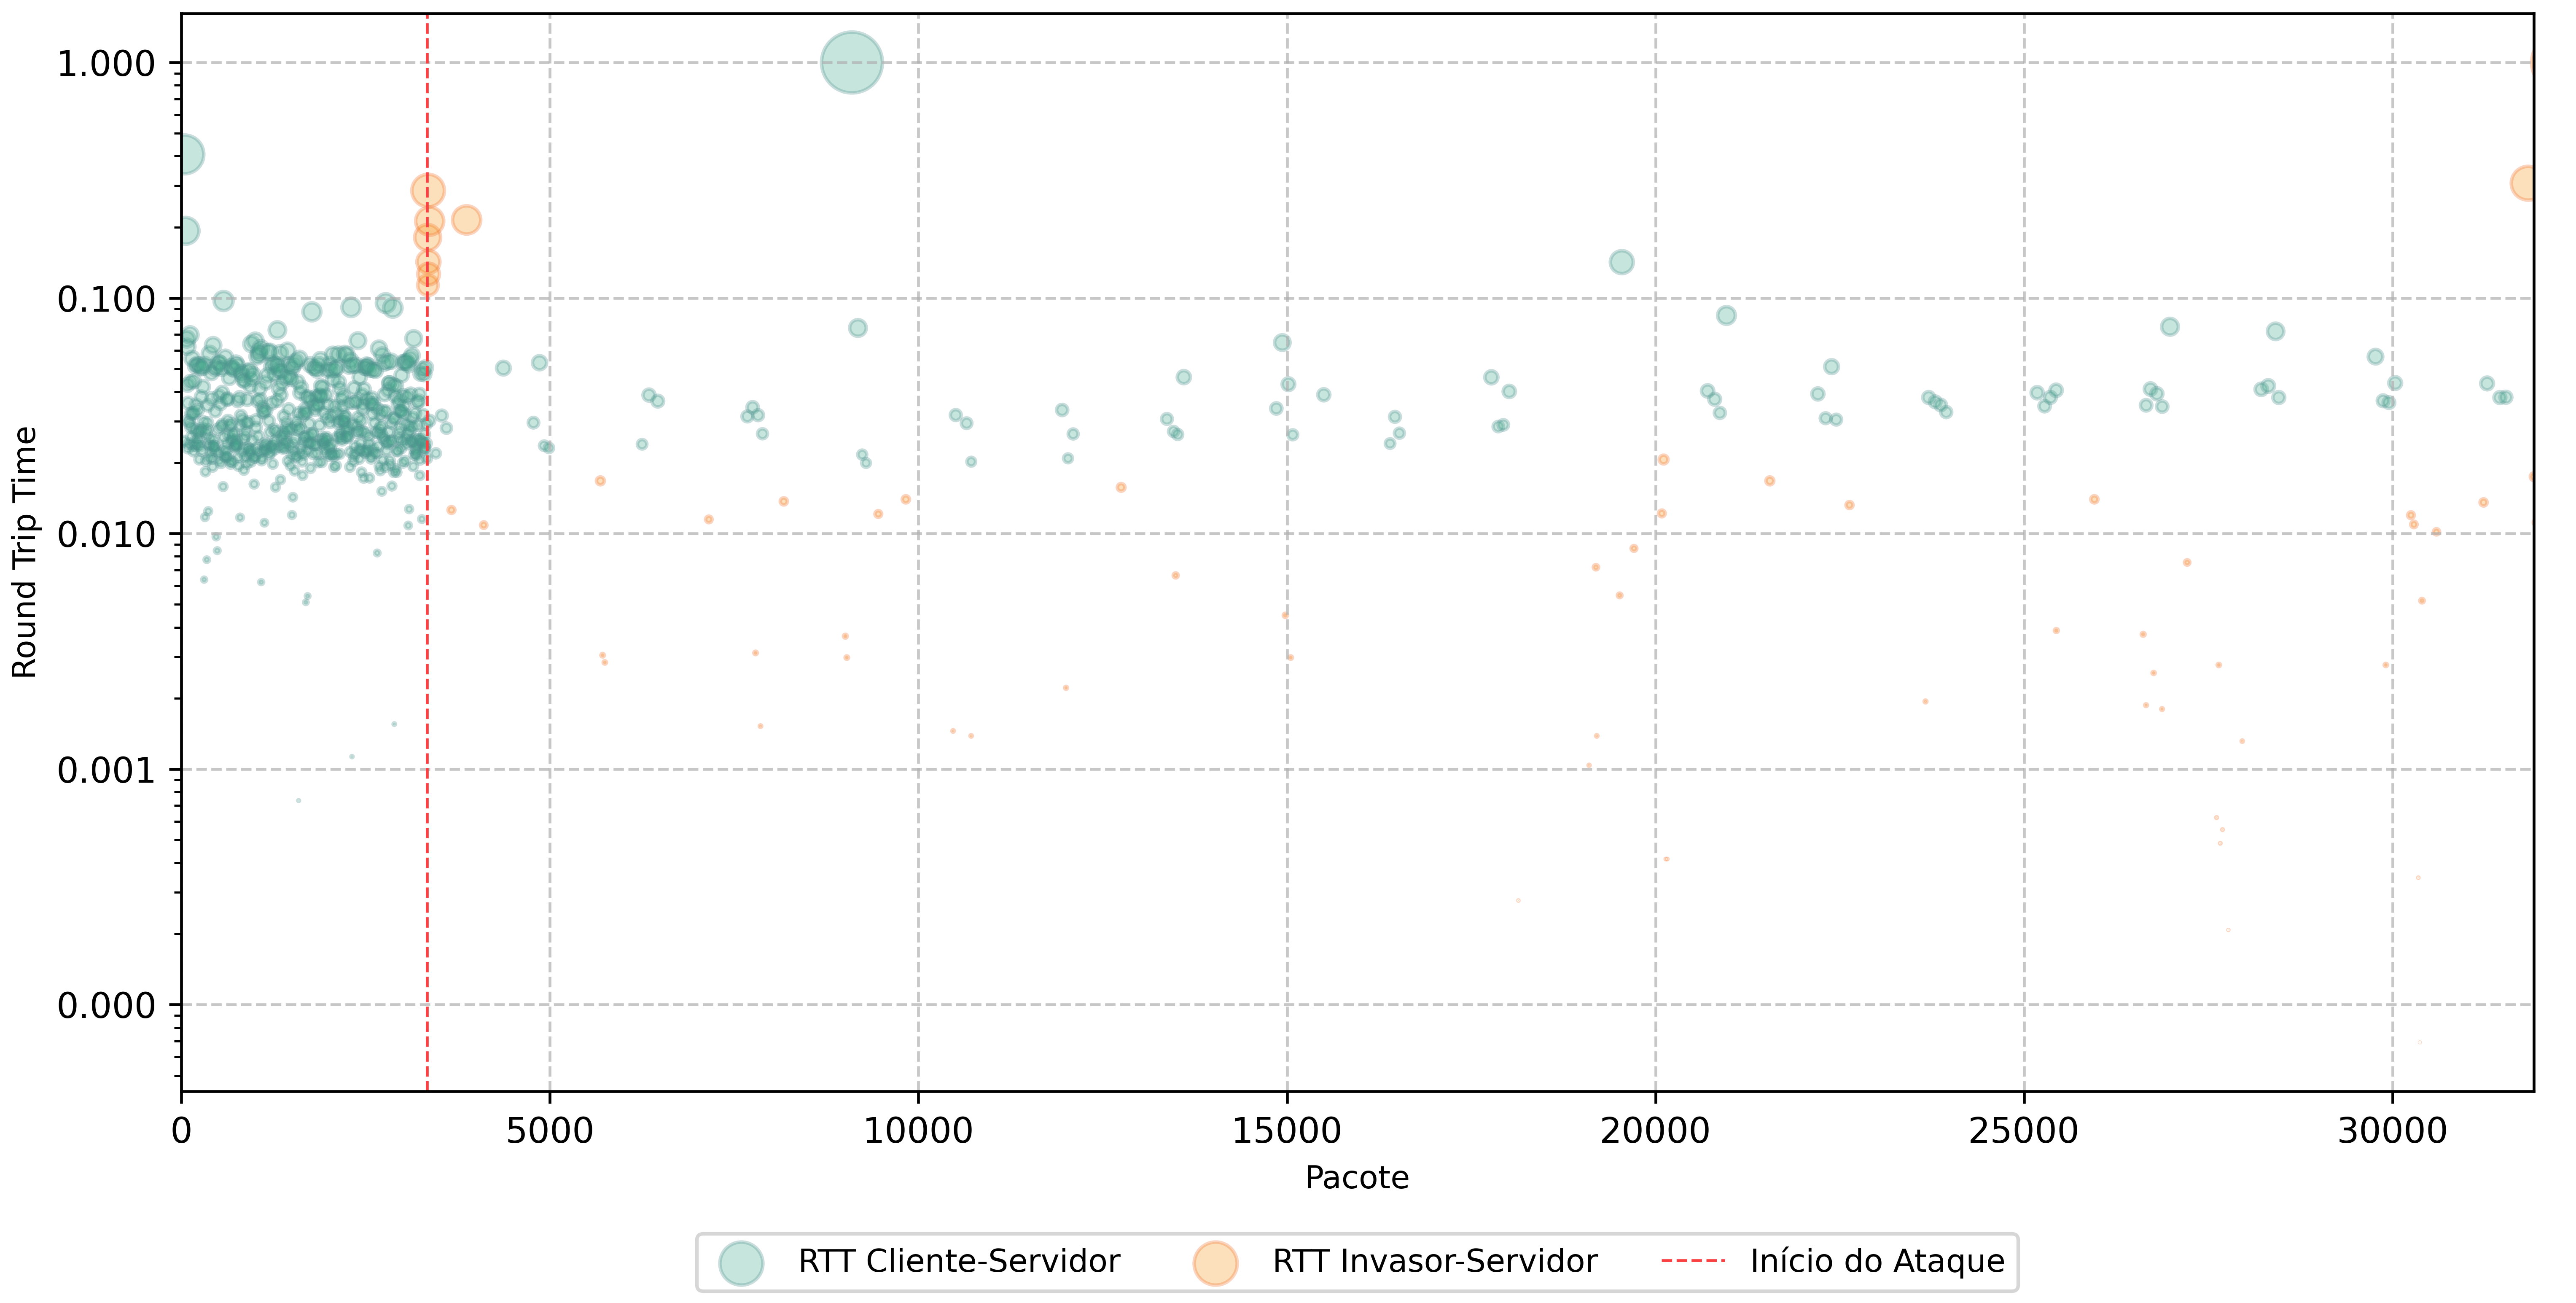
\includegraphics[width=1\textwidth, height=120pt]{USPSC-img/output/cropped/2-dos_function_call_null_deref-rttp.png}
    \end{subfigure}%
    % ~
    % \begin{subfigure}[t]{0.5\textwidth}
    %     \centering
    %     \caption{RTT por segundos}
    %     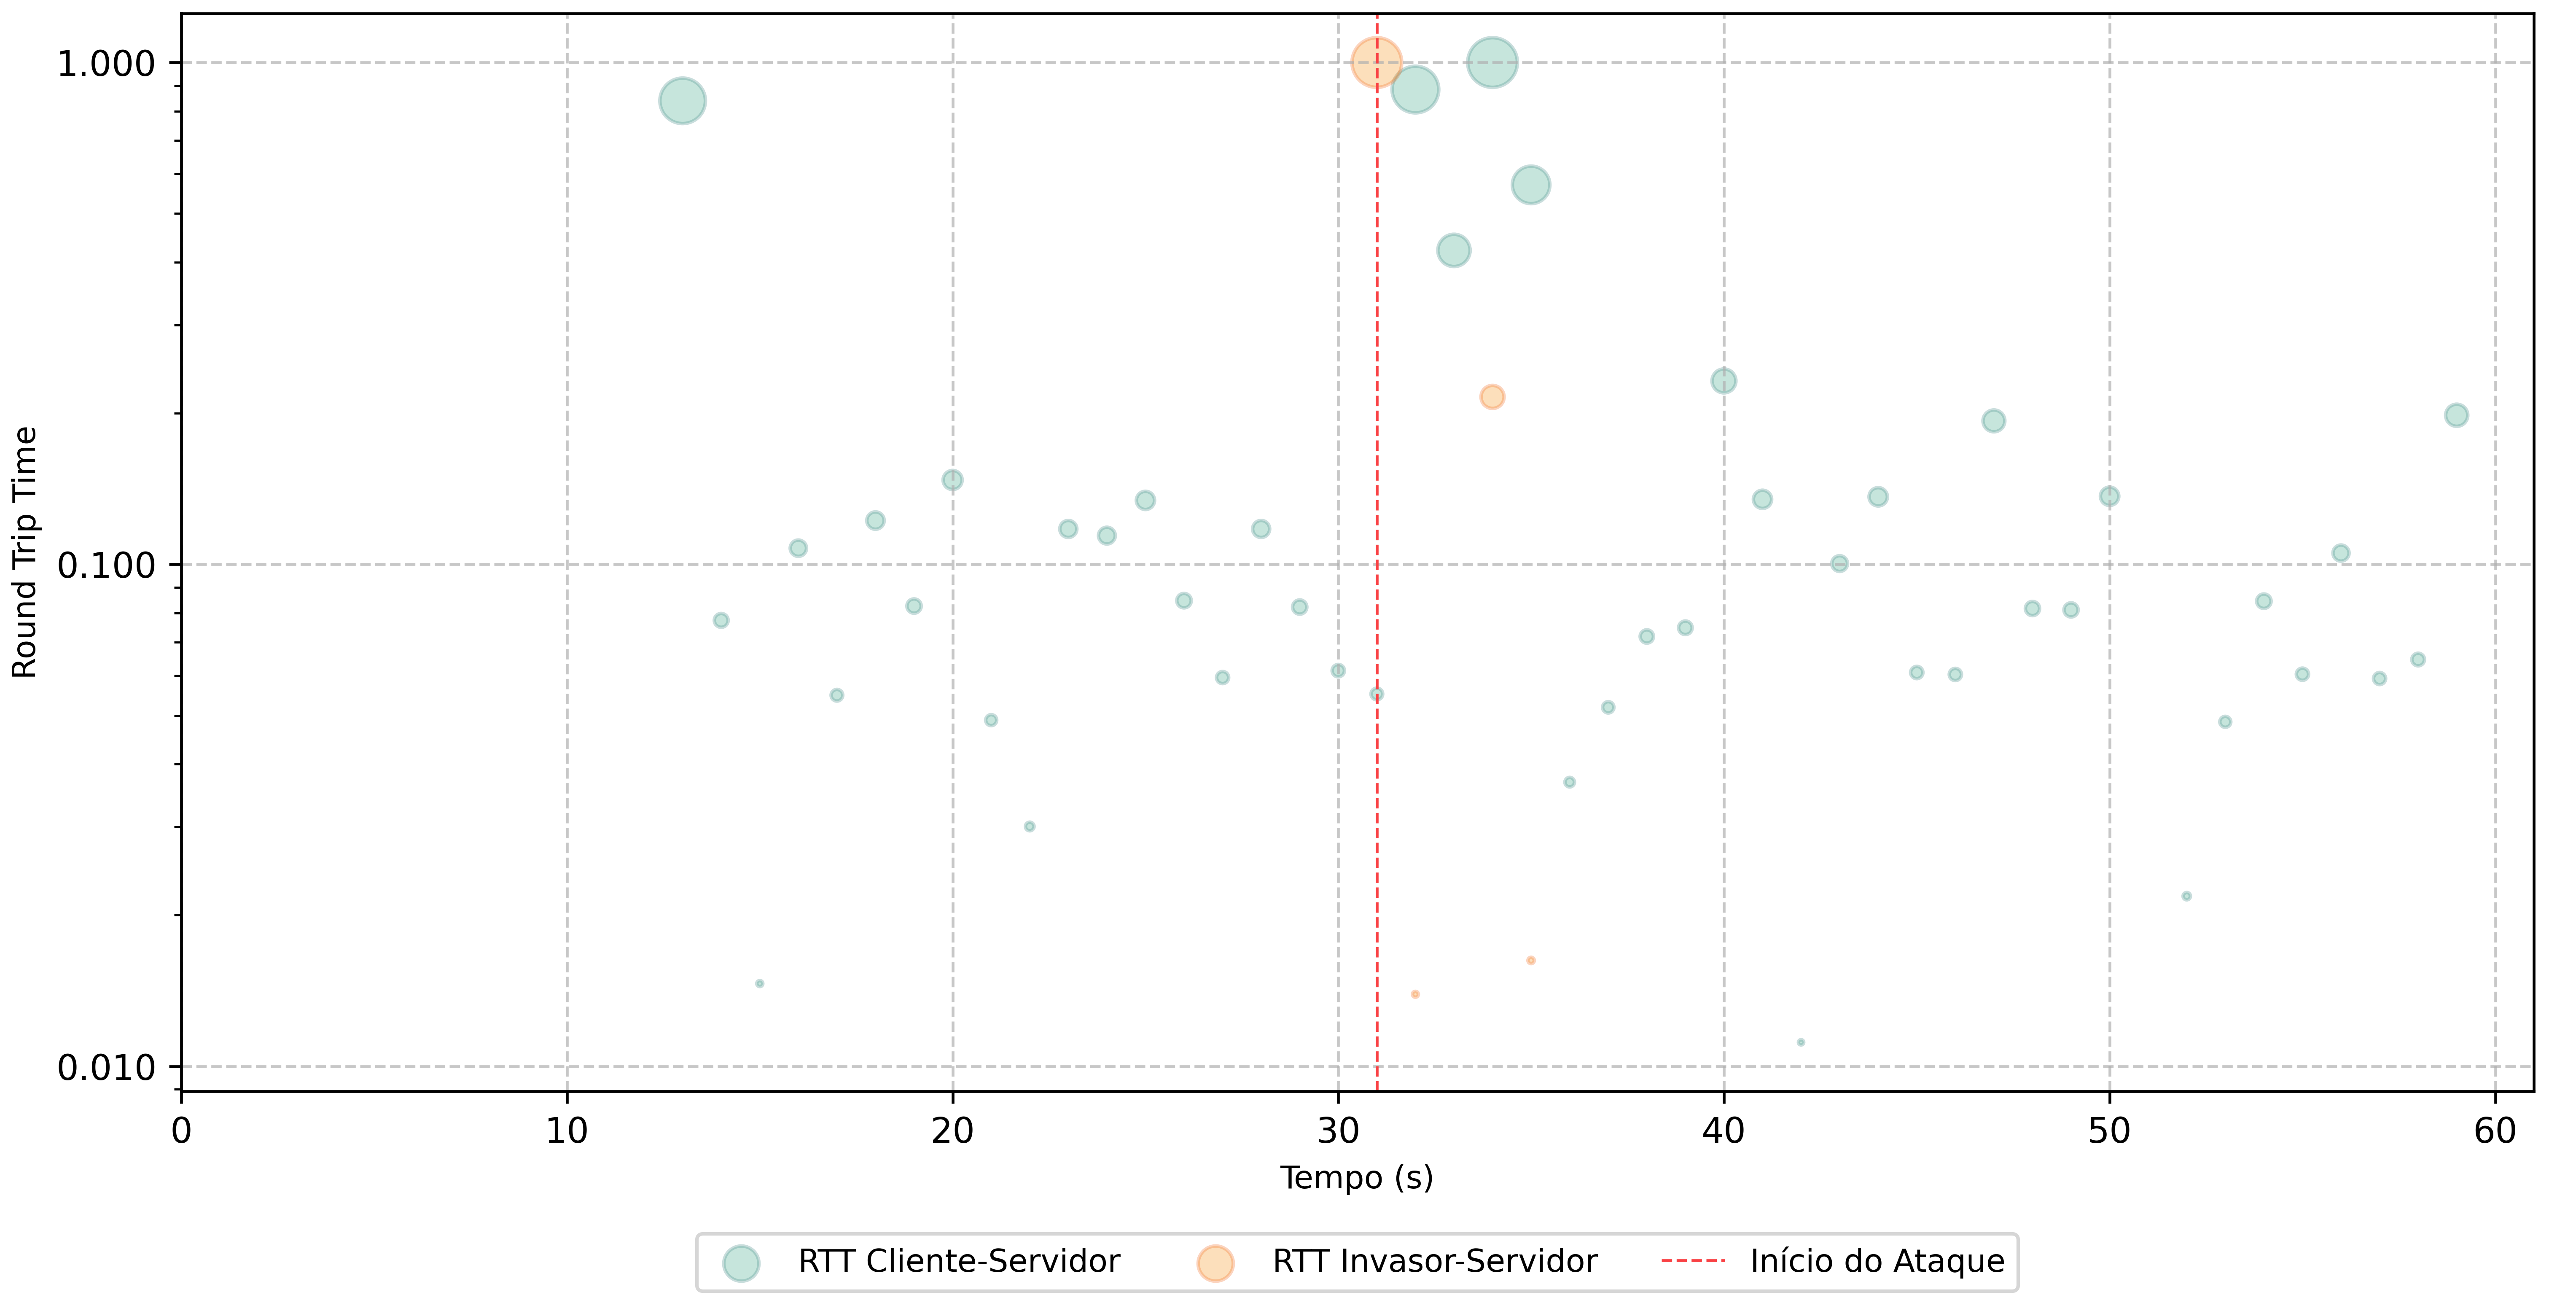
\includegraphics[width=1\textwidth, height=120pt]{USPSC-img/output/cropped/2-dos_function_call_null_deref-rtts.png}
    % \end{subfigure}%
\end{figure}

\begin{figure}[htbp!]
    \centering
    \caption{\label{fig:0-dos_hping3}Gráficos do ataque de DoS por inundação TCP/IP - nível de segurança: `None'.}
    \begin{subfigure}[t]{0.5\textwidth}
        \centering
        \caption{\textit{Throughput}}
        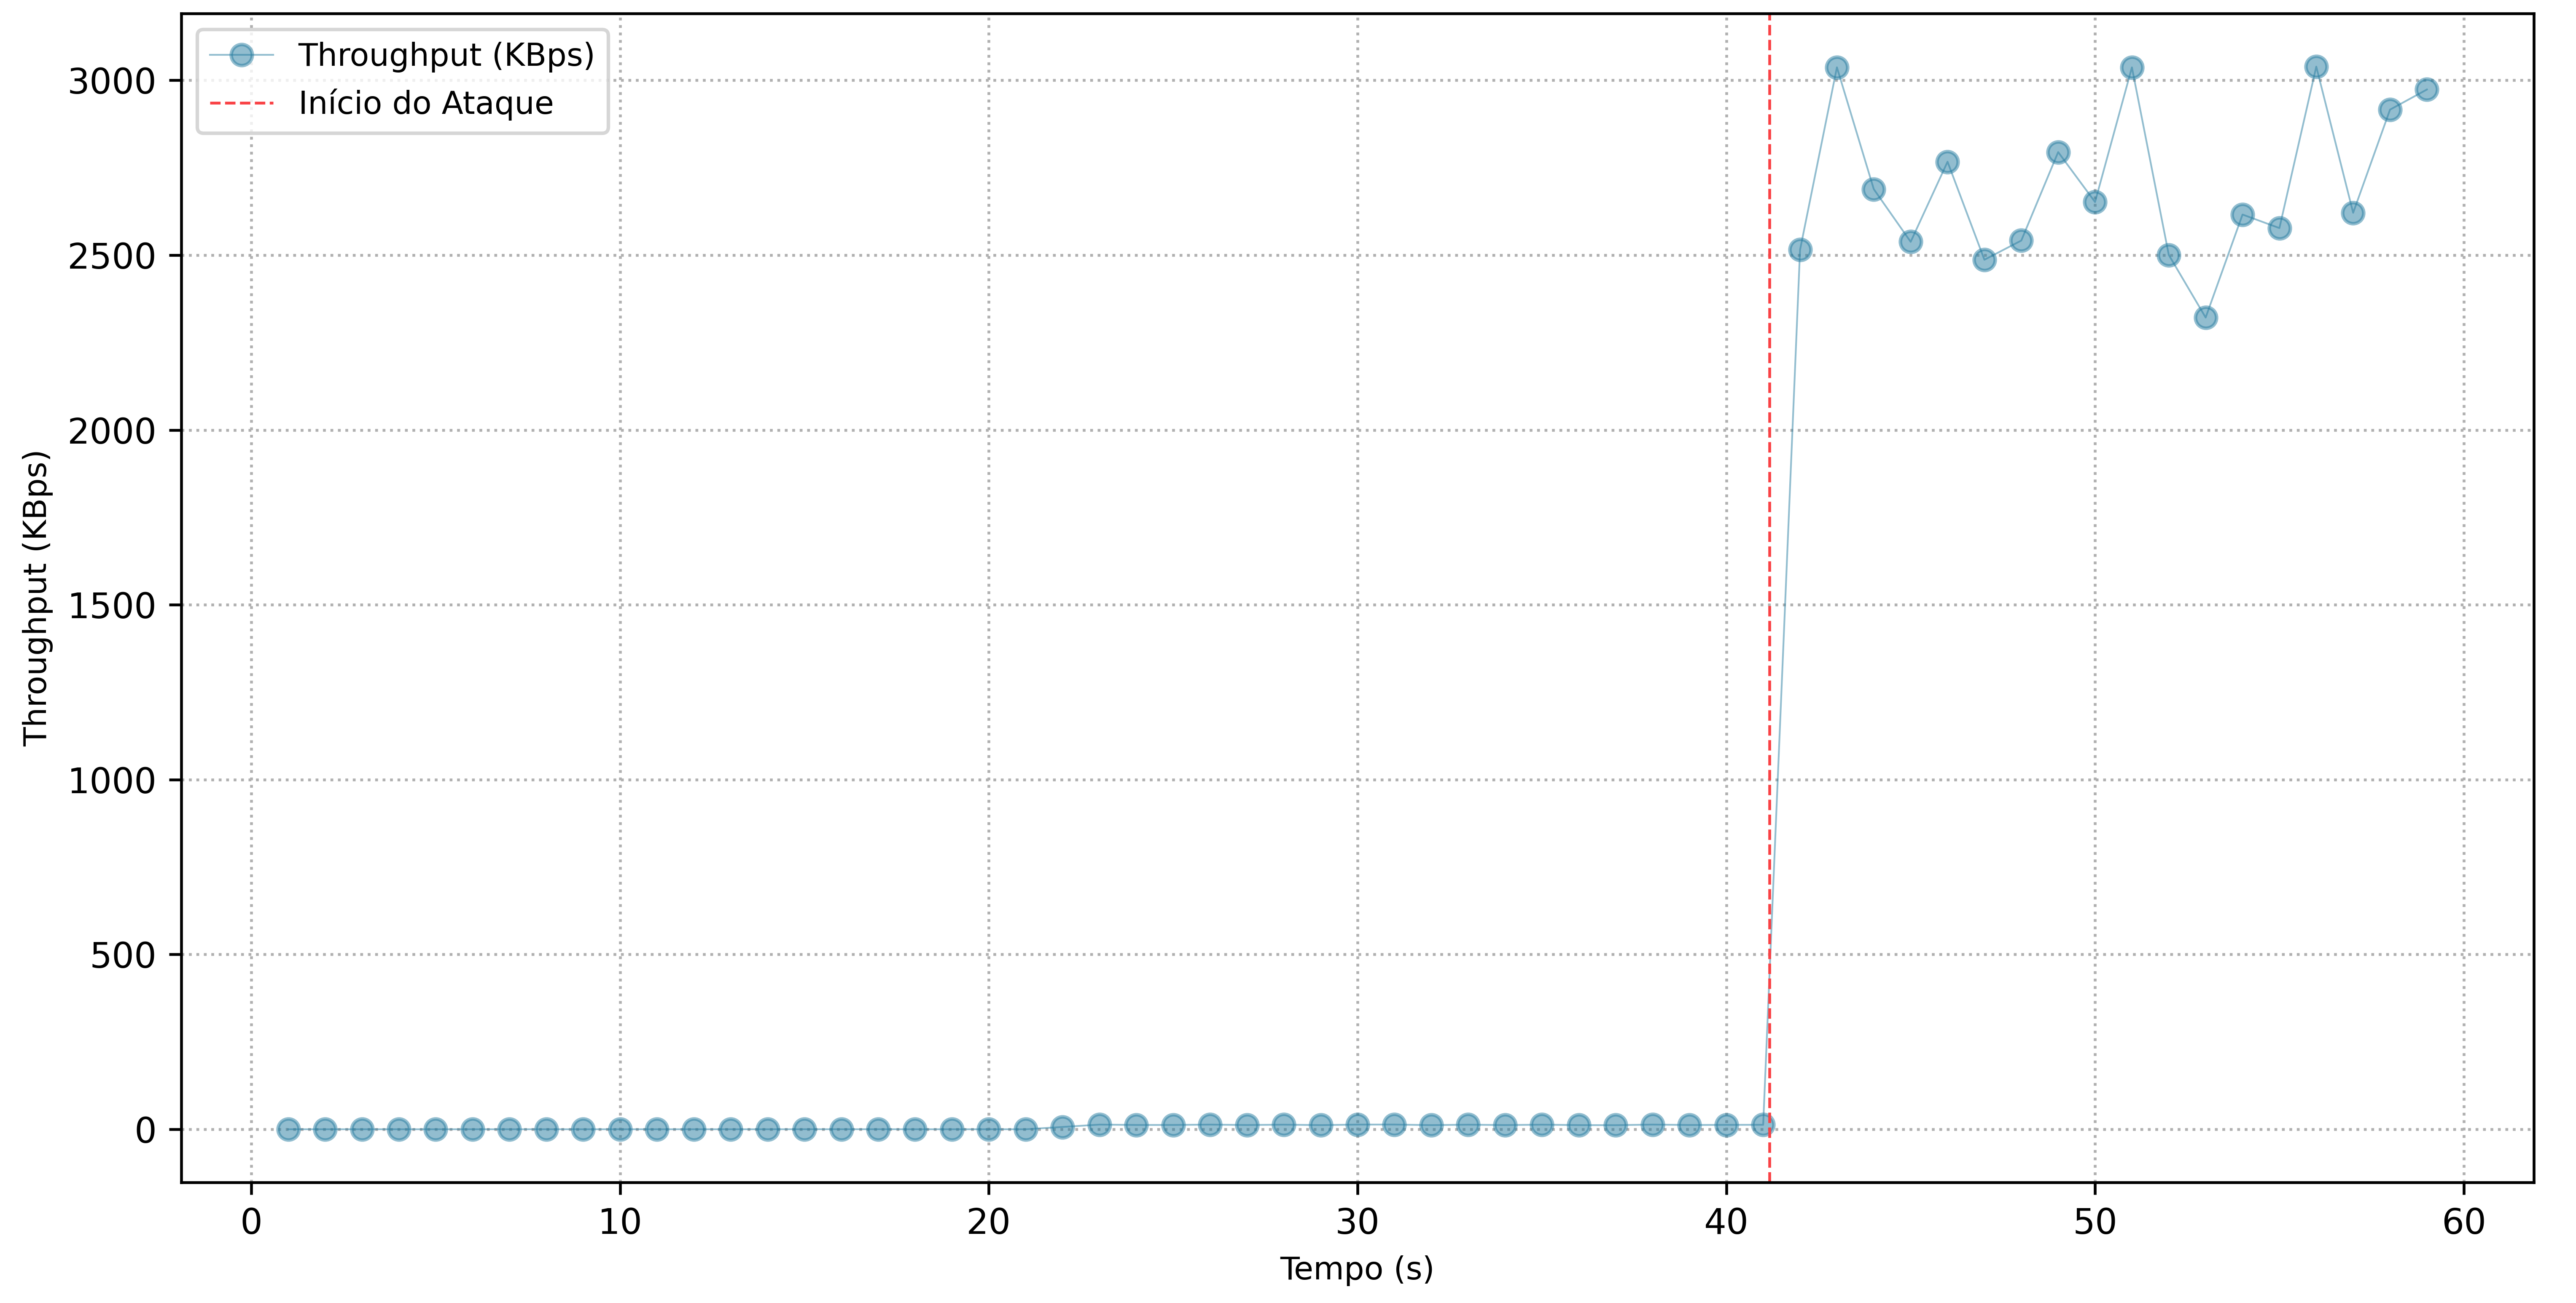
\includegraphics[width=1\textwidth, height=120pt]{USPSC-img/output/cropped/0-dos_hping3-tput.png}
    \end{subfigure}%
    ~ 
    \begin{subfigure}[t]{0.5\textwidth}
        \centering
        \caption{Desempenho}
        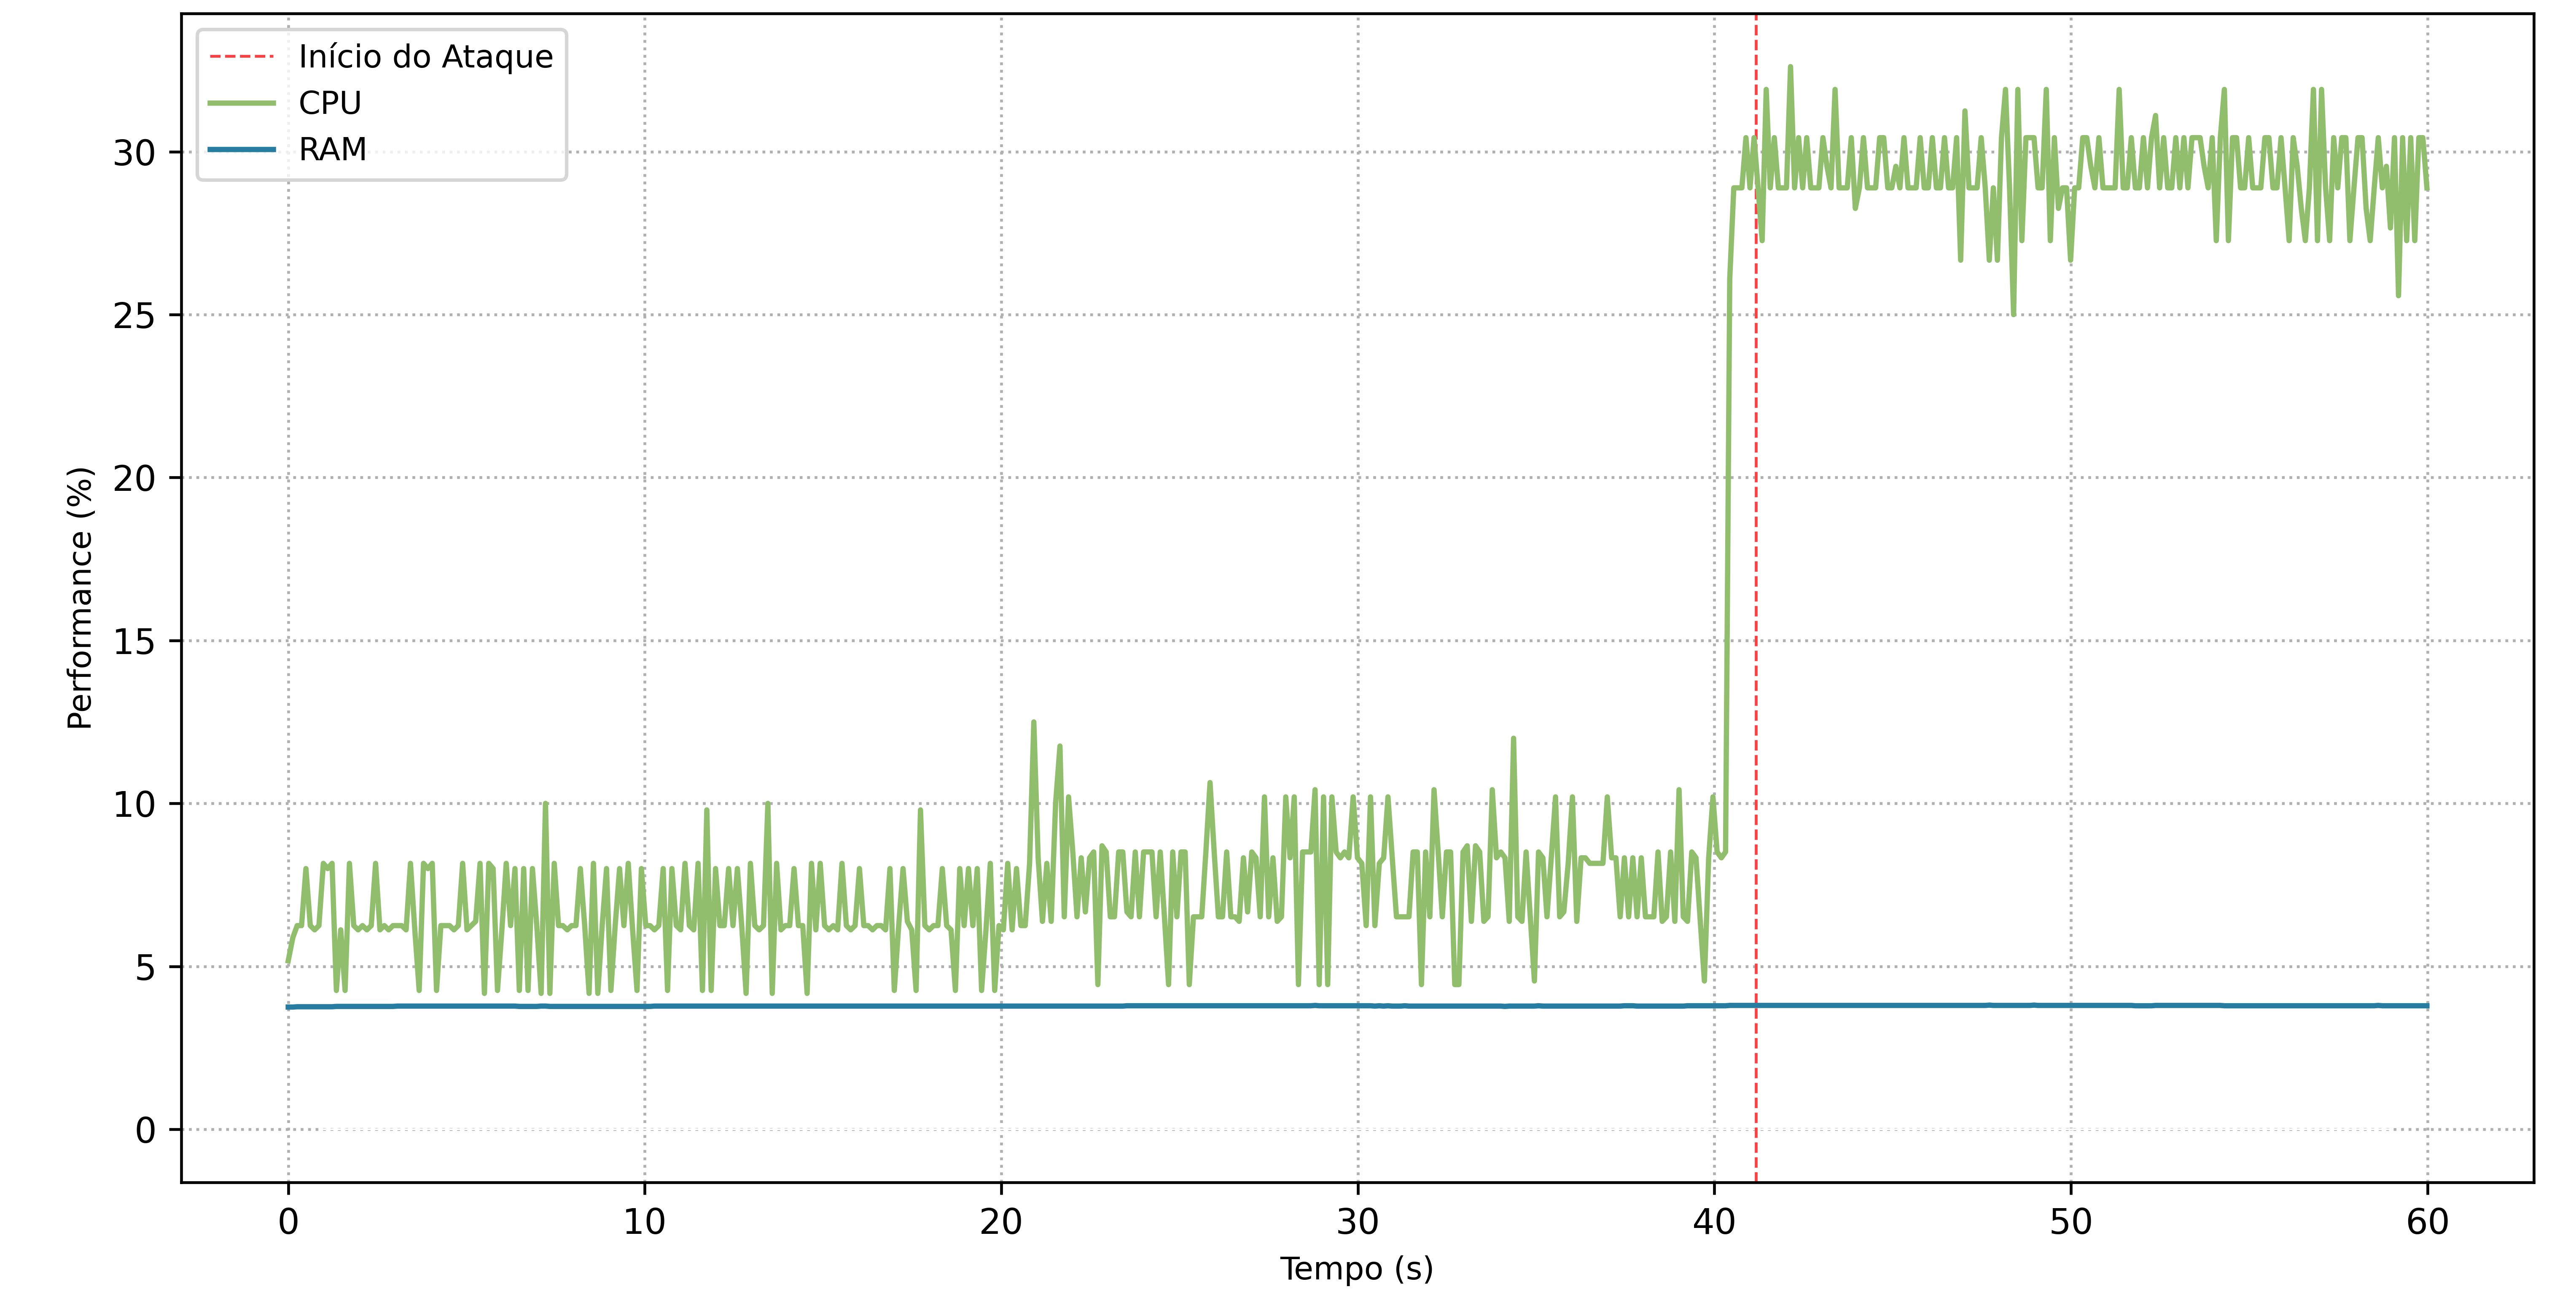
\includegraphics[width=1\textwidth, height=120pt]{USPSC-img/output/cropped/0-dos_hping3-perf.png}
    \end{subfigure}%
    \\
    \begin{subfigure}[t]{0.5\textwidth}
        \centering
        \caption{Pacotes OPC UA}
        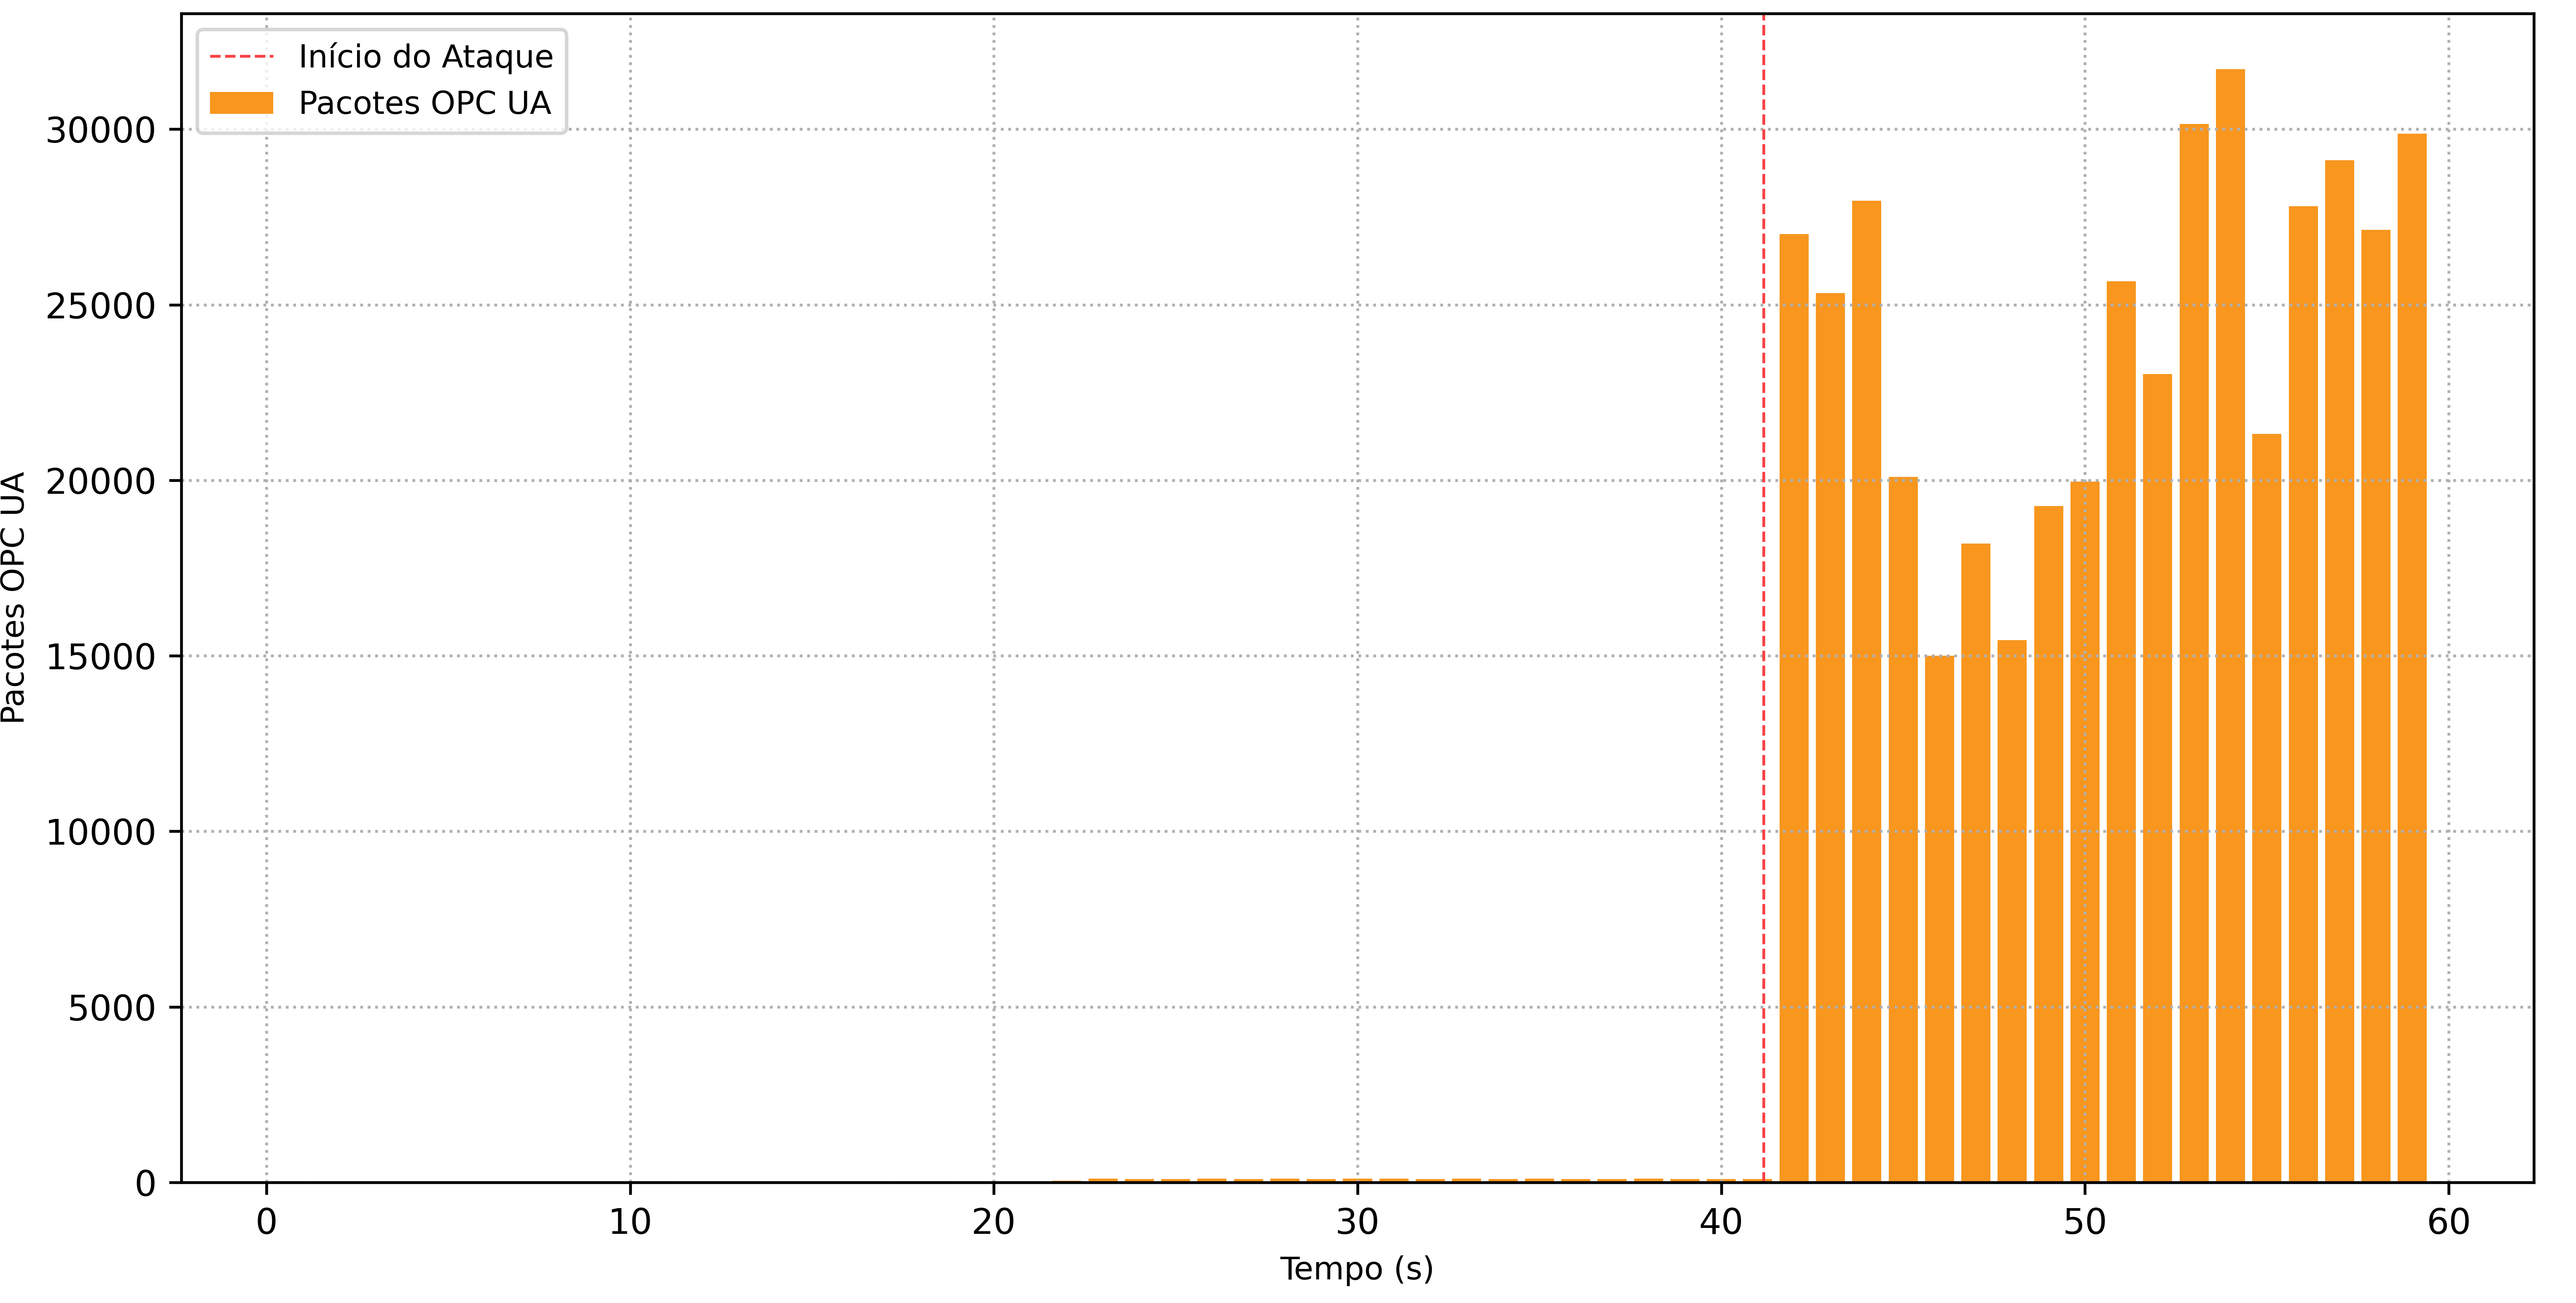
\includegraphics[width=1\textwidth, height=120pt]{USPSC-img/output/cropped/0-dos_hping3-pack.png}
    \end{subfigure}%
    ~
    \begin{subfigure}[t]{0.5\textwidth}
        \centering
        \caption{RTT por pacote}
        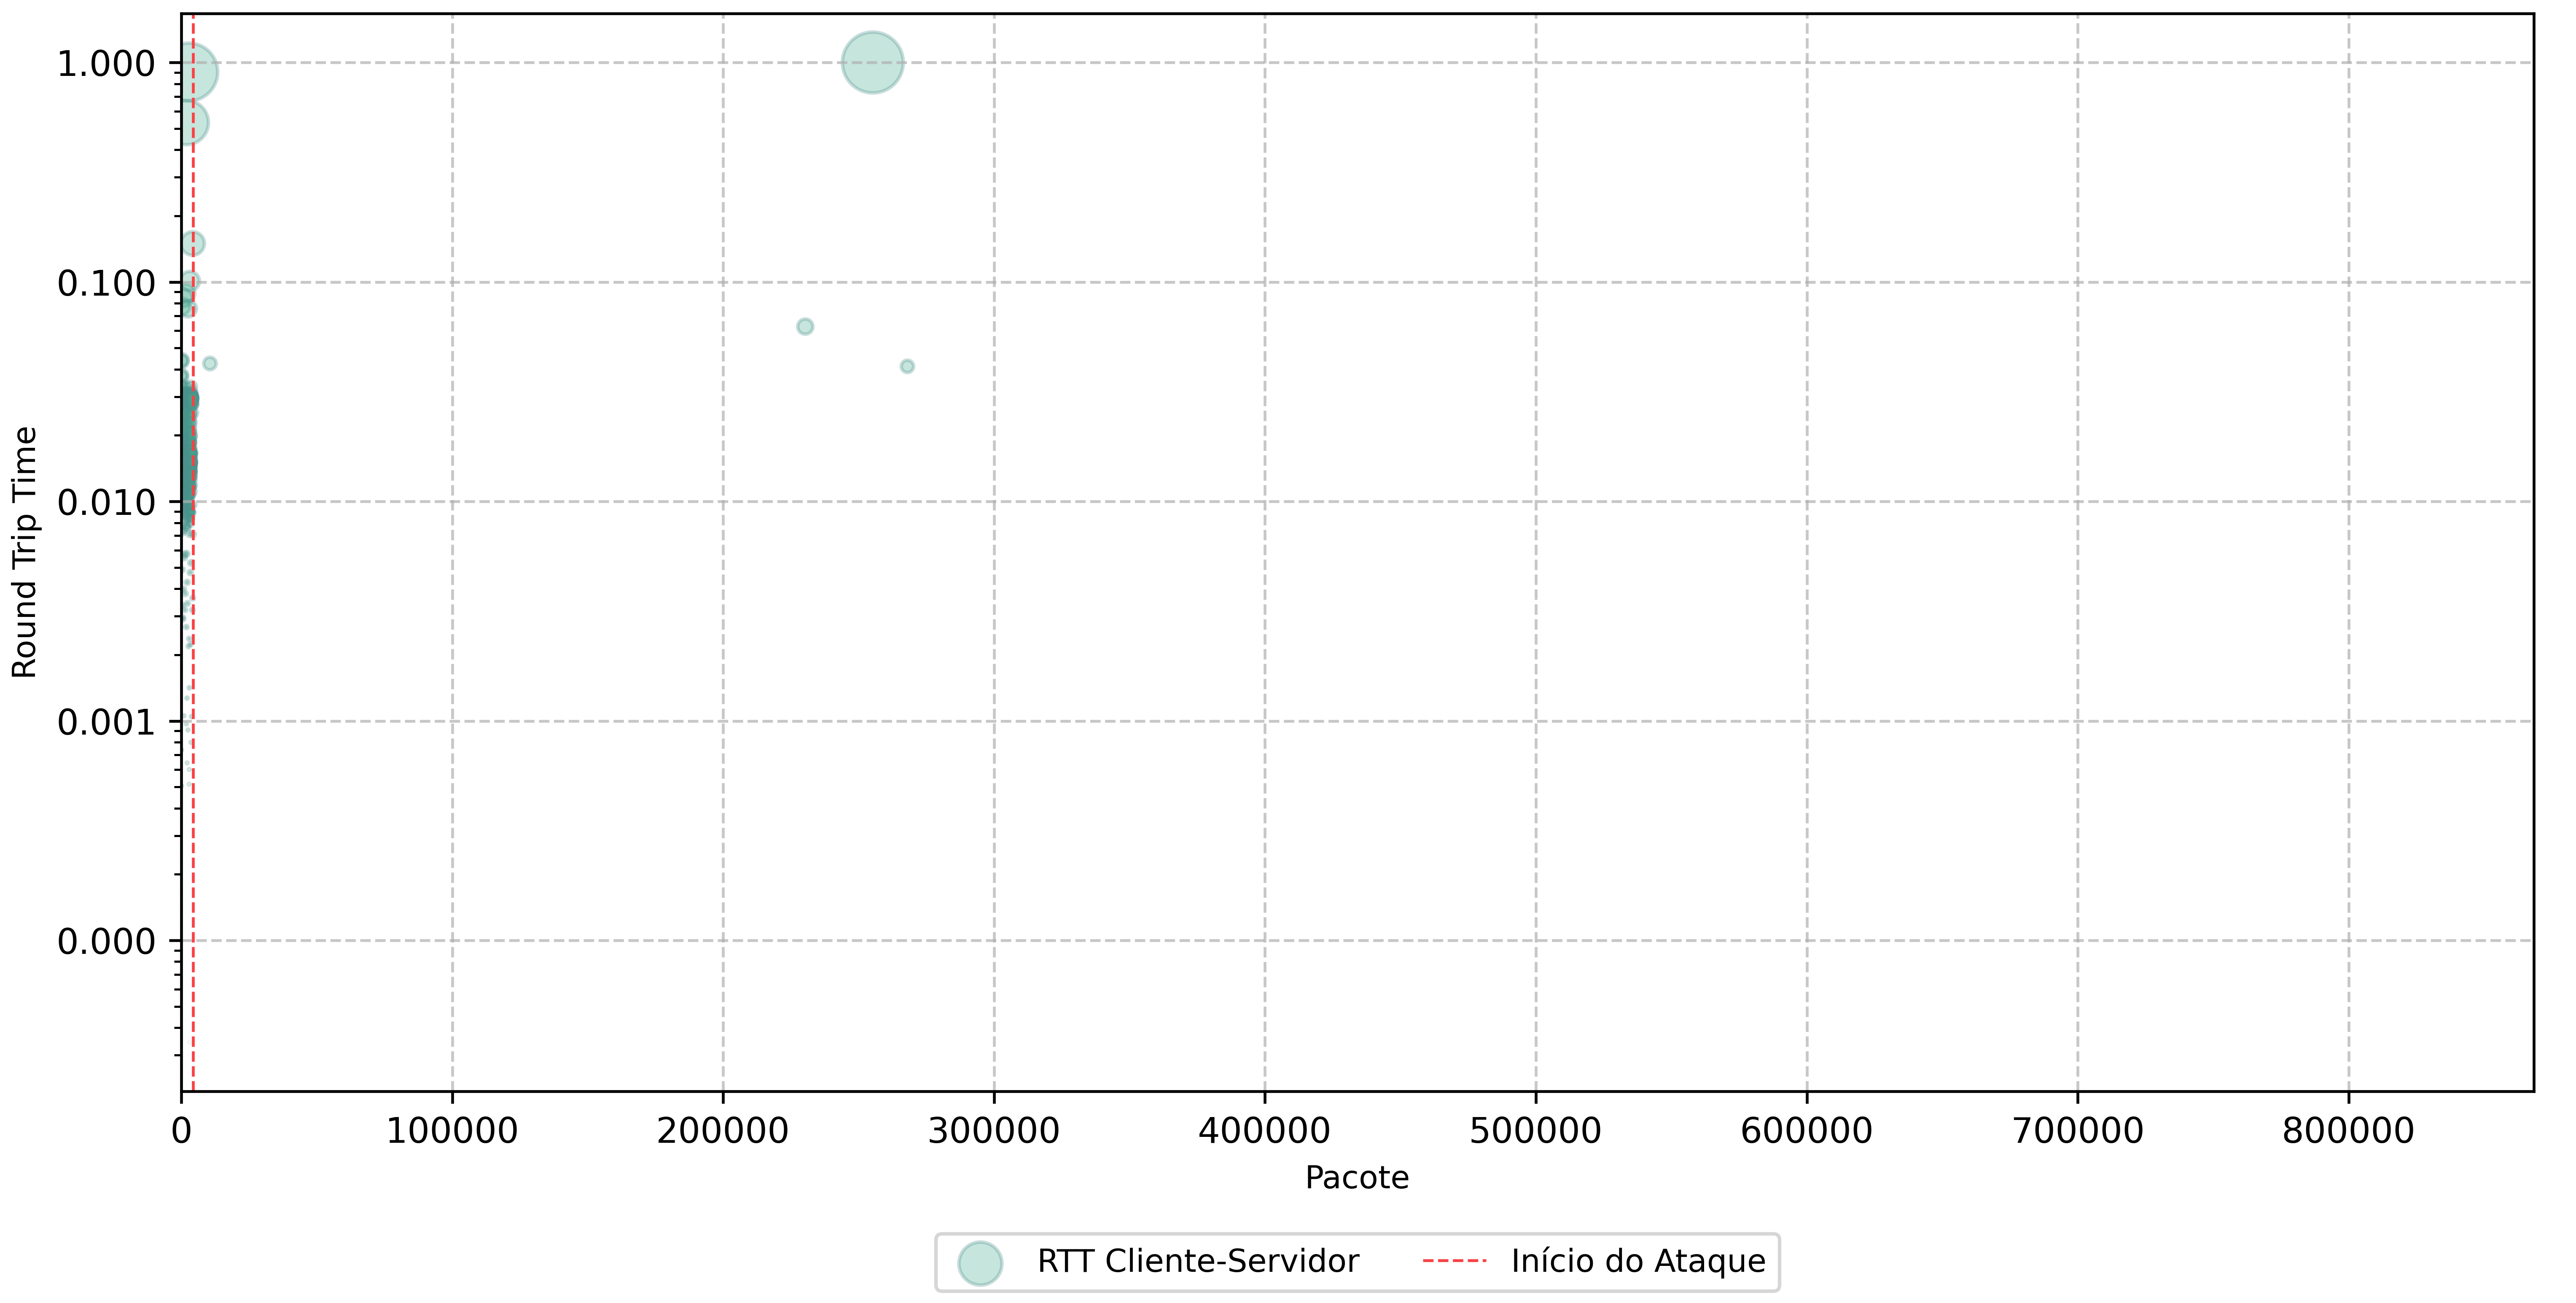
\includegraphics[width=1\textwidth, height=120pt]{USPSC-img/output/cropped/0-dos_hping3-rttp.png}
    \end{subfigure}%
    % ~
    % \begin{subfigure}[t]{0.5\textwidth}
    %     \centering
    %     \caption{RTT por segundos}
    %     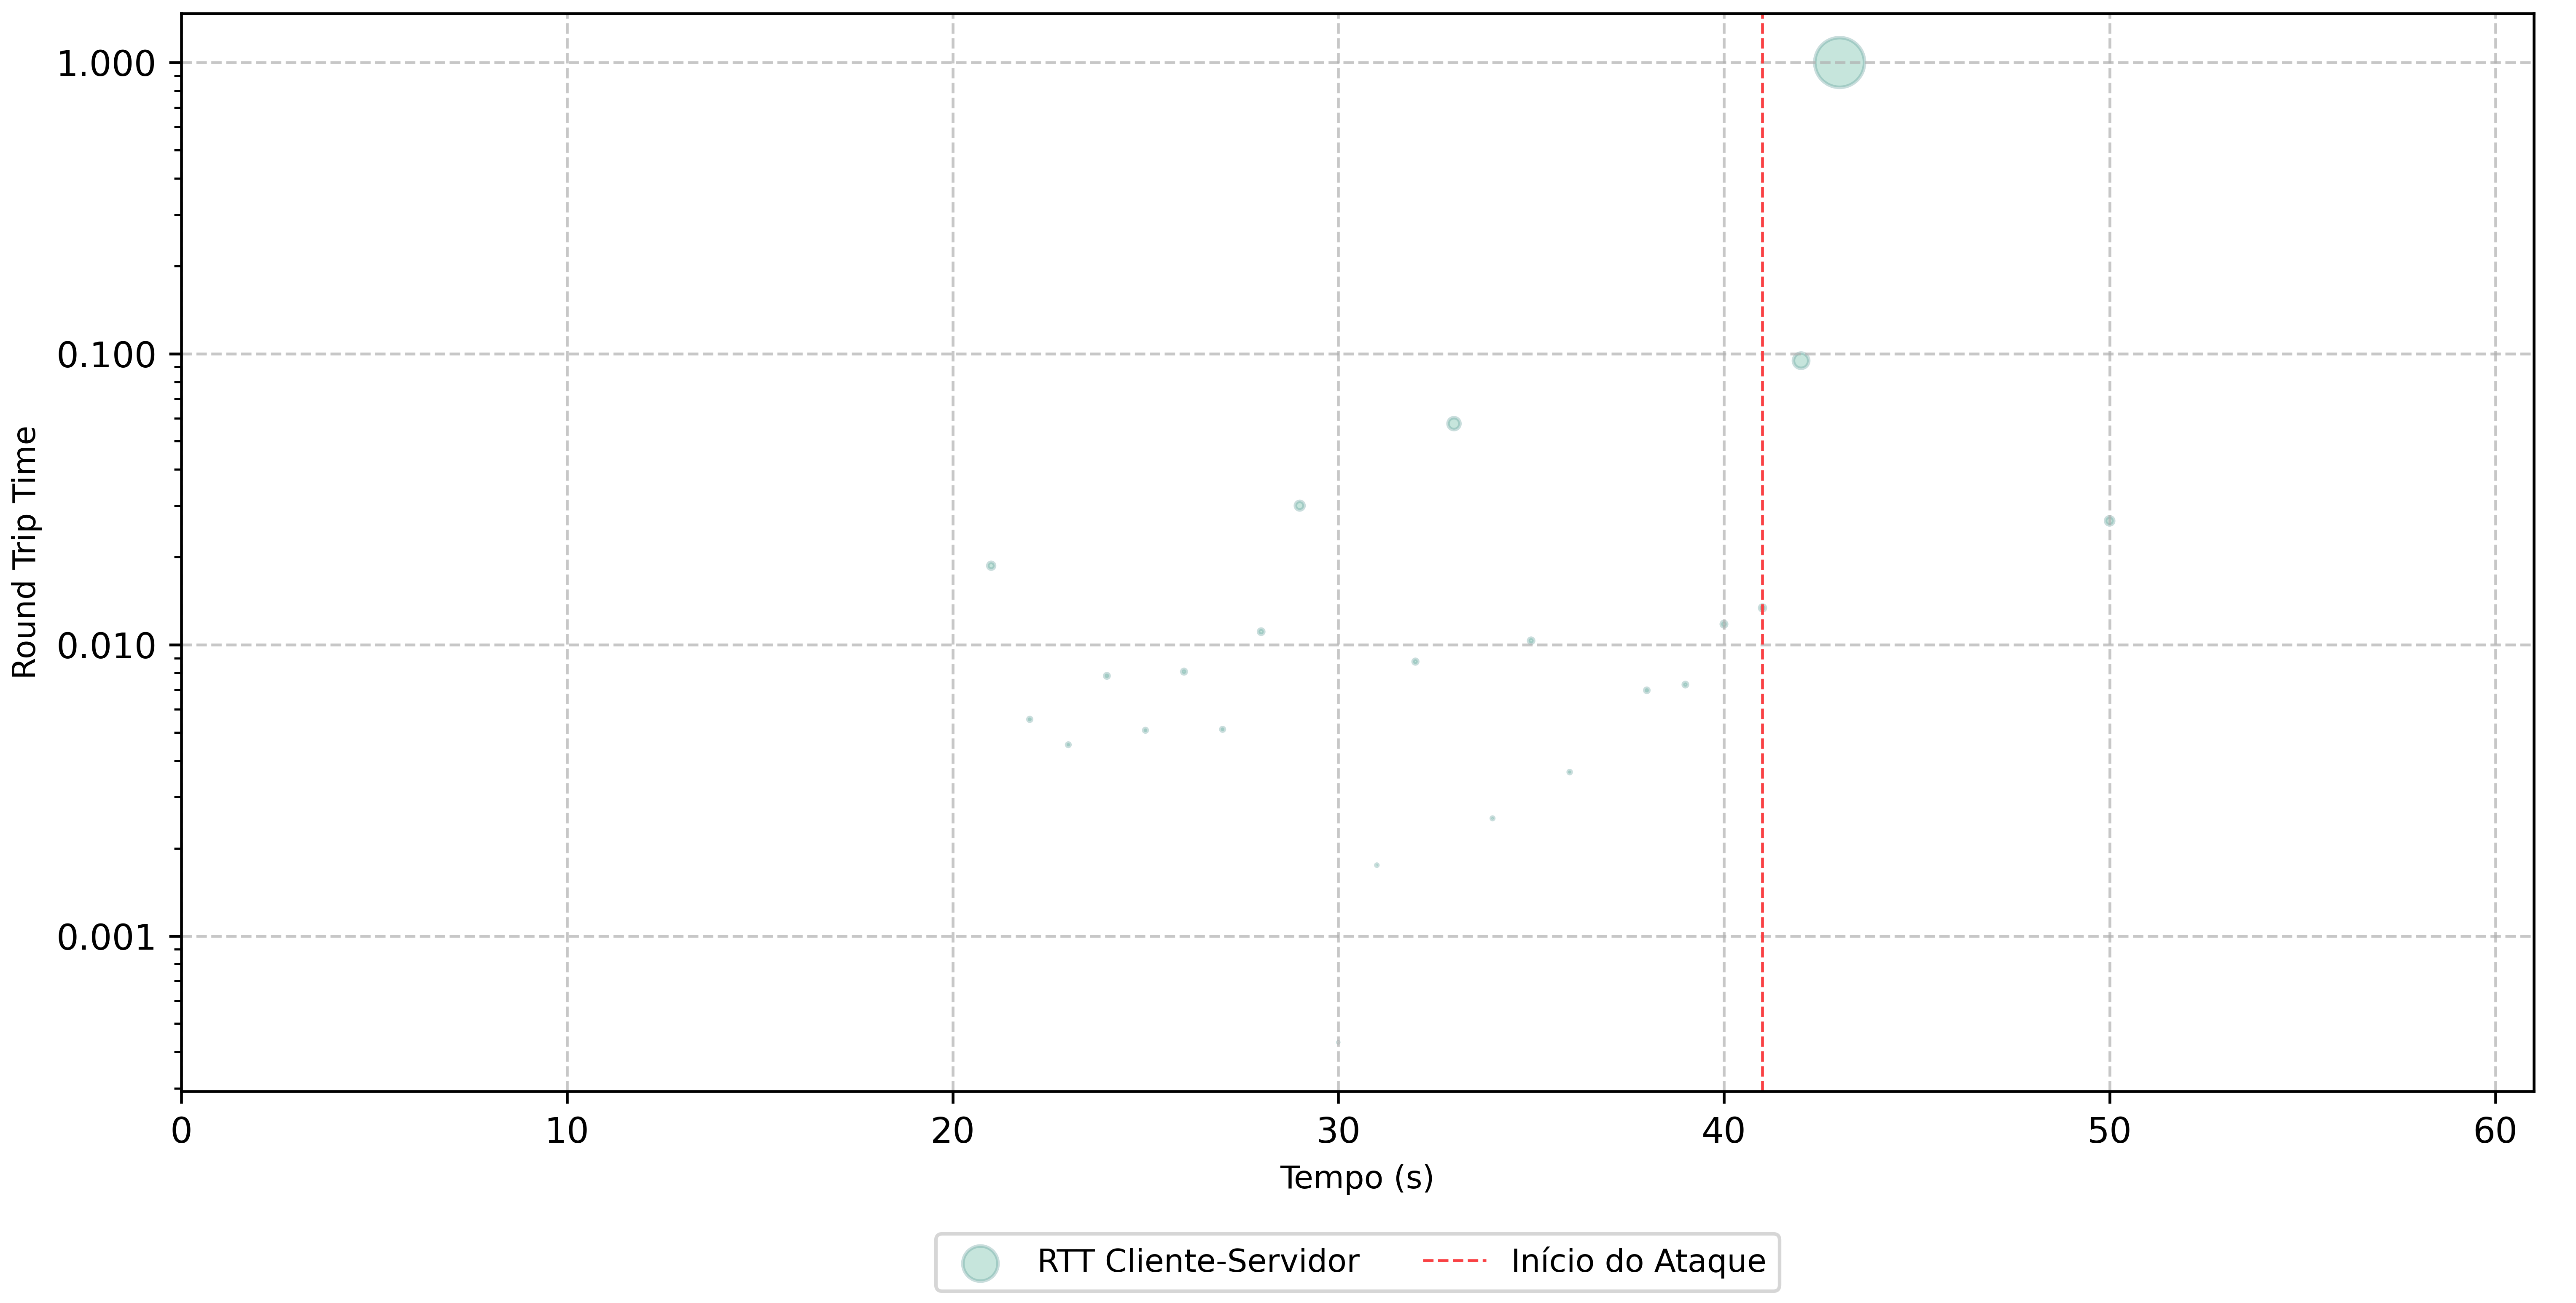
\includegraphics[width=1\textwidth, height=120pt]{USPSC-img/output/cropped/0-dos_hping3-rtts.png}
    % \end{subfigure}%
\end{figure}

\begin{figure}[htbp!]
    \centering
    \caption{\label{fig:1-dos_hping3}Gráficos do ataque de DoS por inundação TCP/IP - nível de segurança: `Sign'.}
    \begin{subfigure}[t]{0.5\textwidth}
        \centering
        \caption{\textit{Throughput}}
        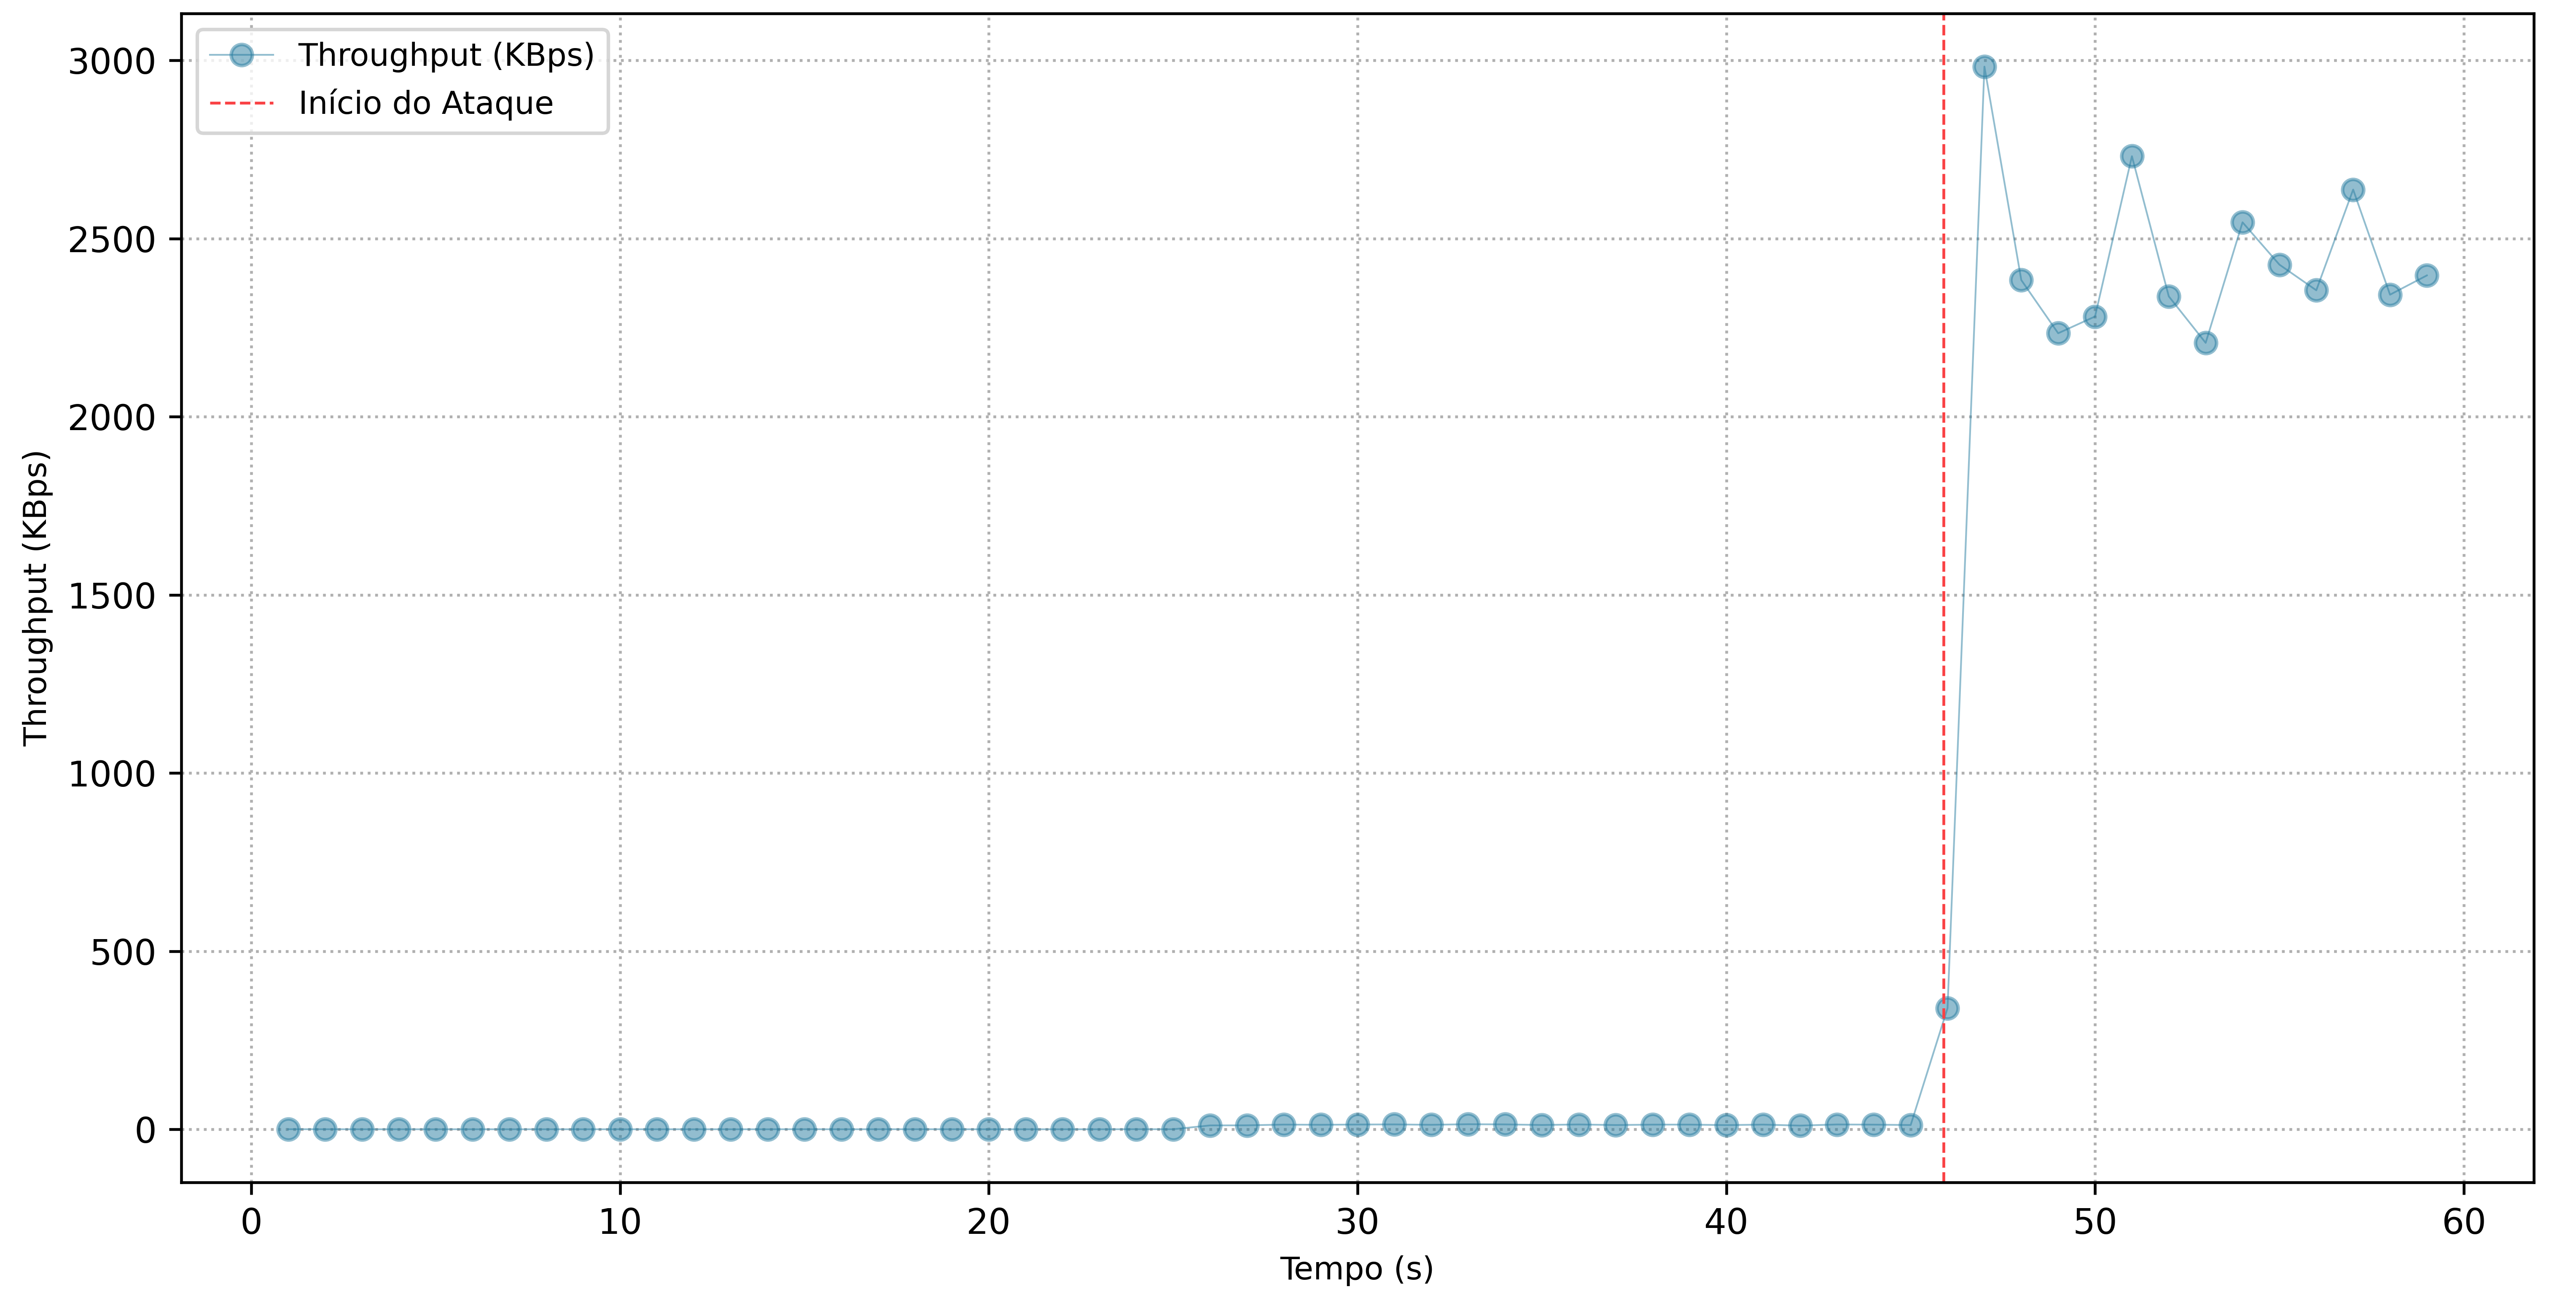
\includegraphics[width=1\textwidth, height=120pt]{USPSC-img/output/cropped/1-dos_hping3-tput.png}
    \end{subfigure}%
    ~ 
    \begin{subfigure}[t]{0.5\textwidth}
        \centering
        \caption{Desempenho}
        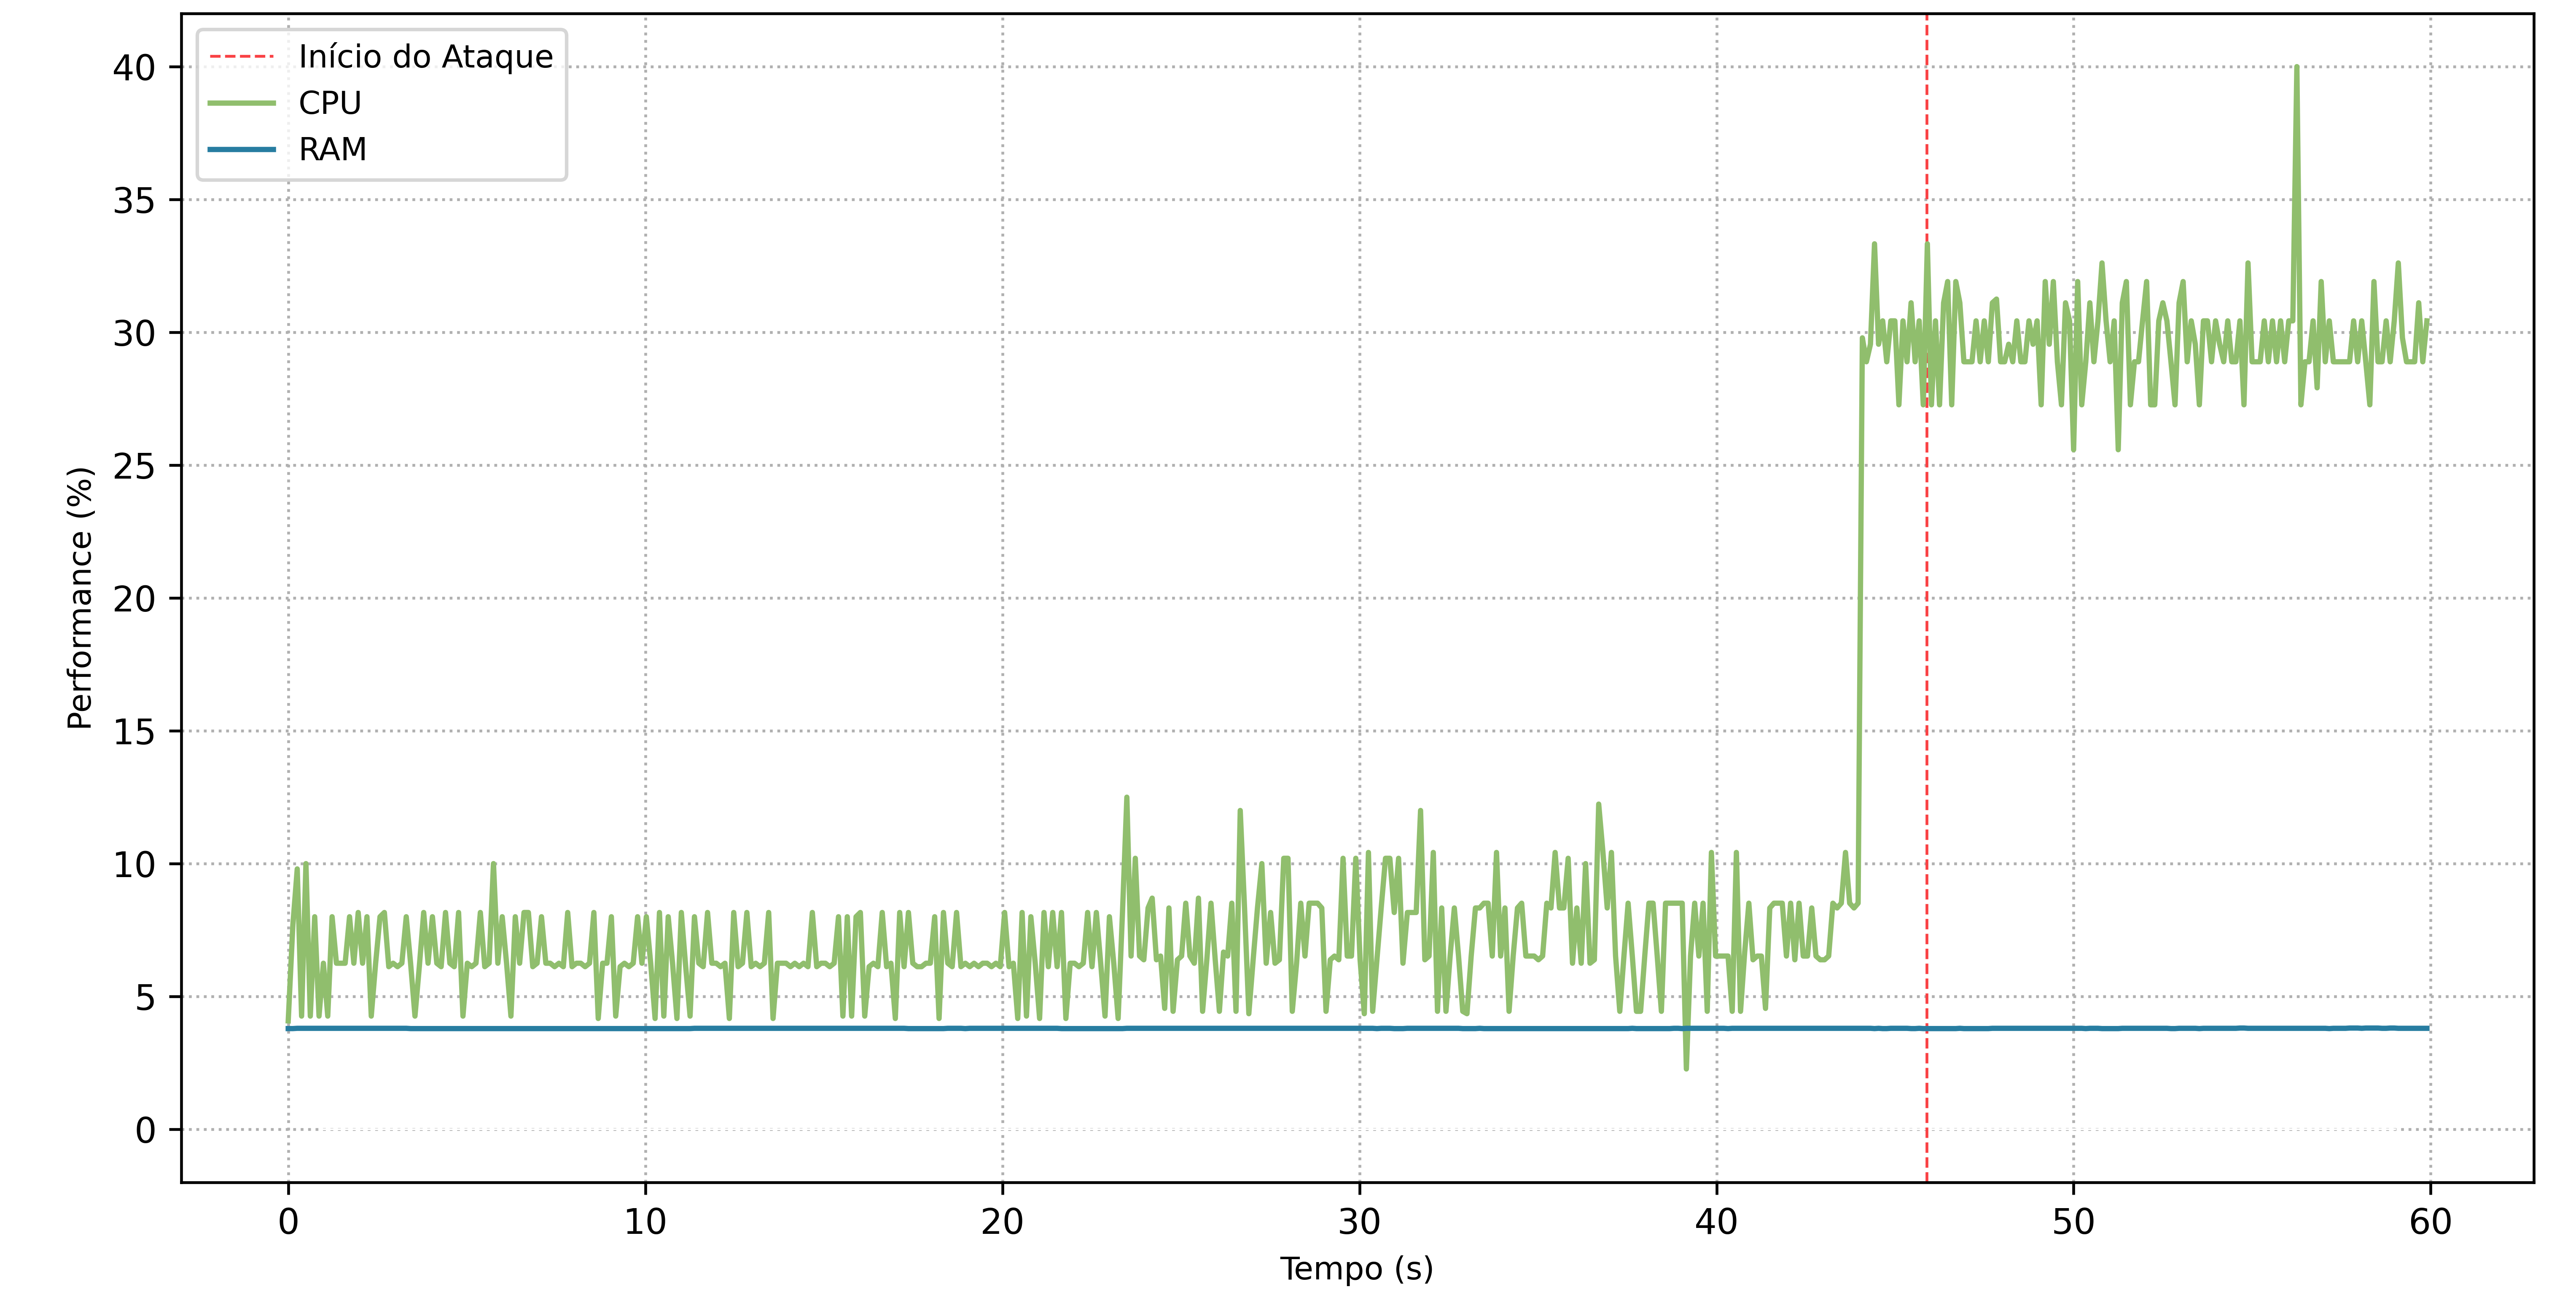
\includegraphics[width=1\textwidth, height=120pt]{USPSC-img/output/cropped/1-dos_hping3-perf.png}
    \end{subfigure}%
    \\
    \begin{subfigure}[t]{0.5\textwidth}
        \centering
        \caption{Pacotes OPC UA}
        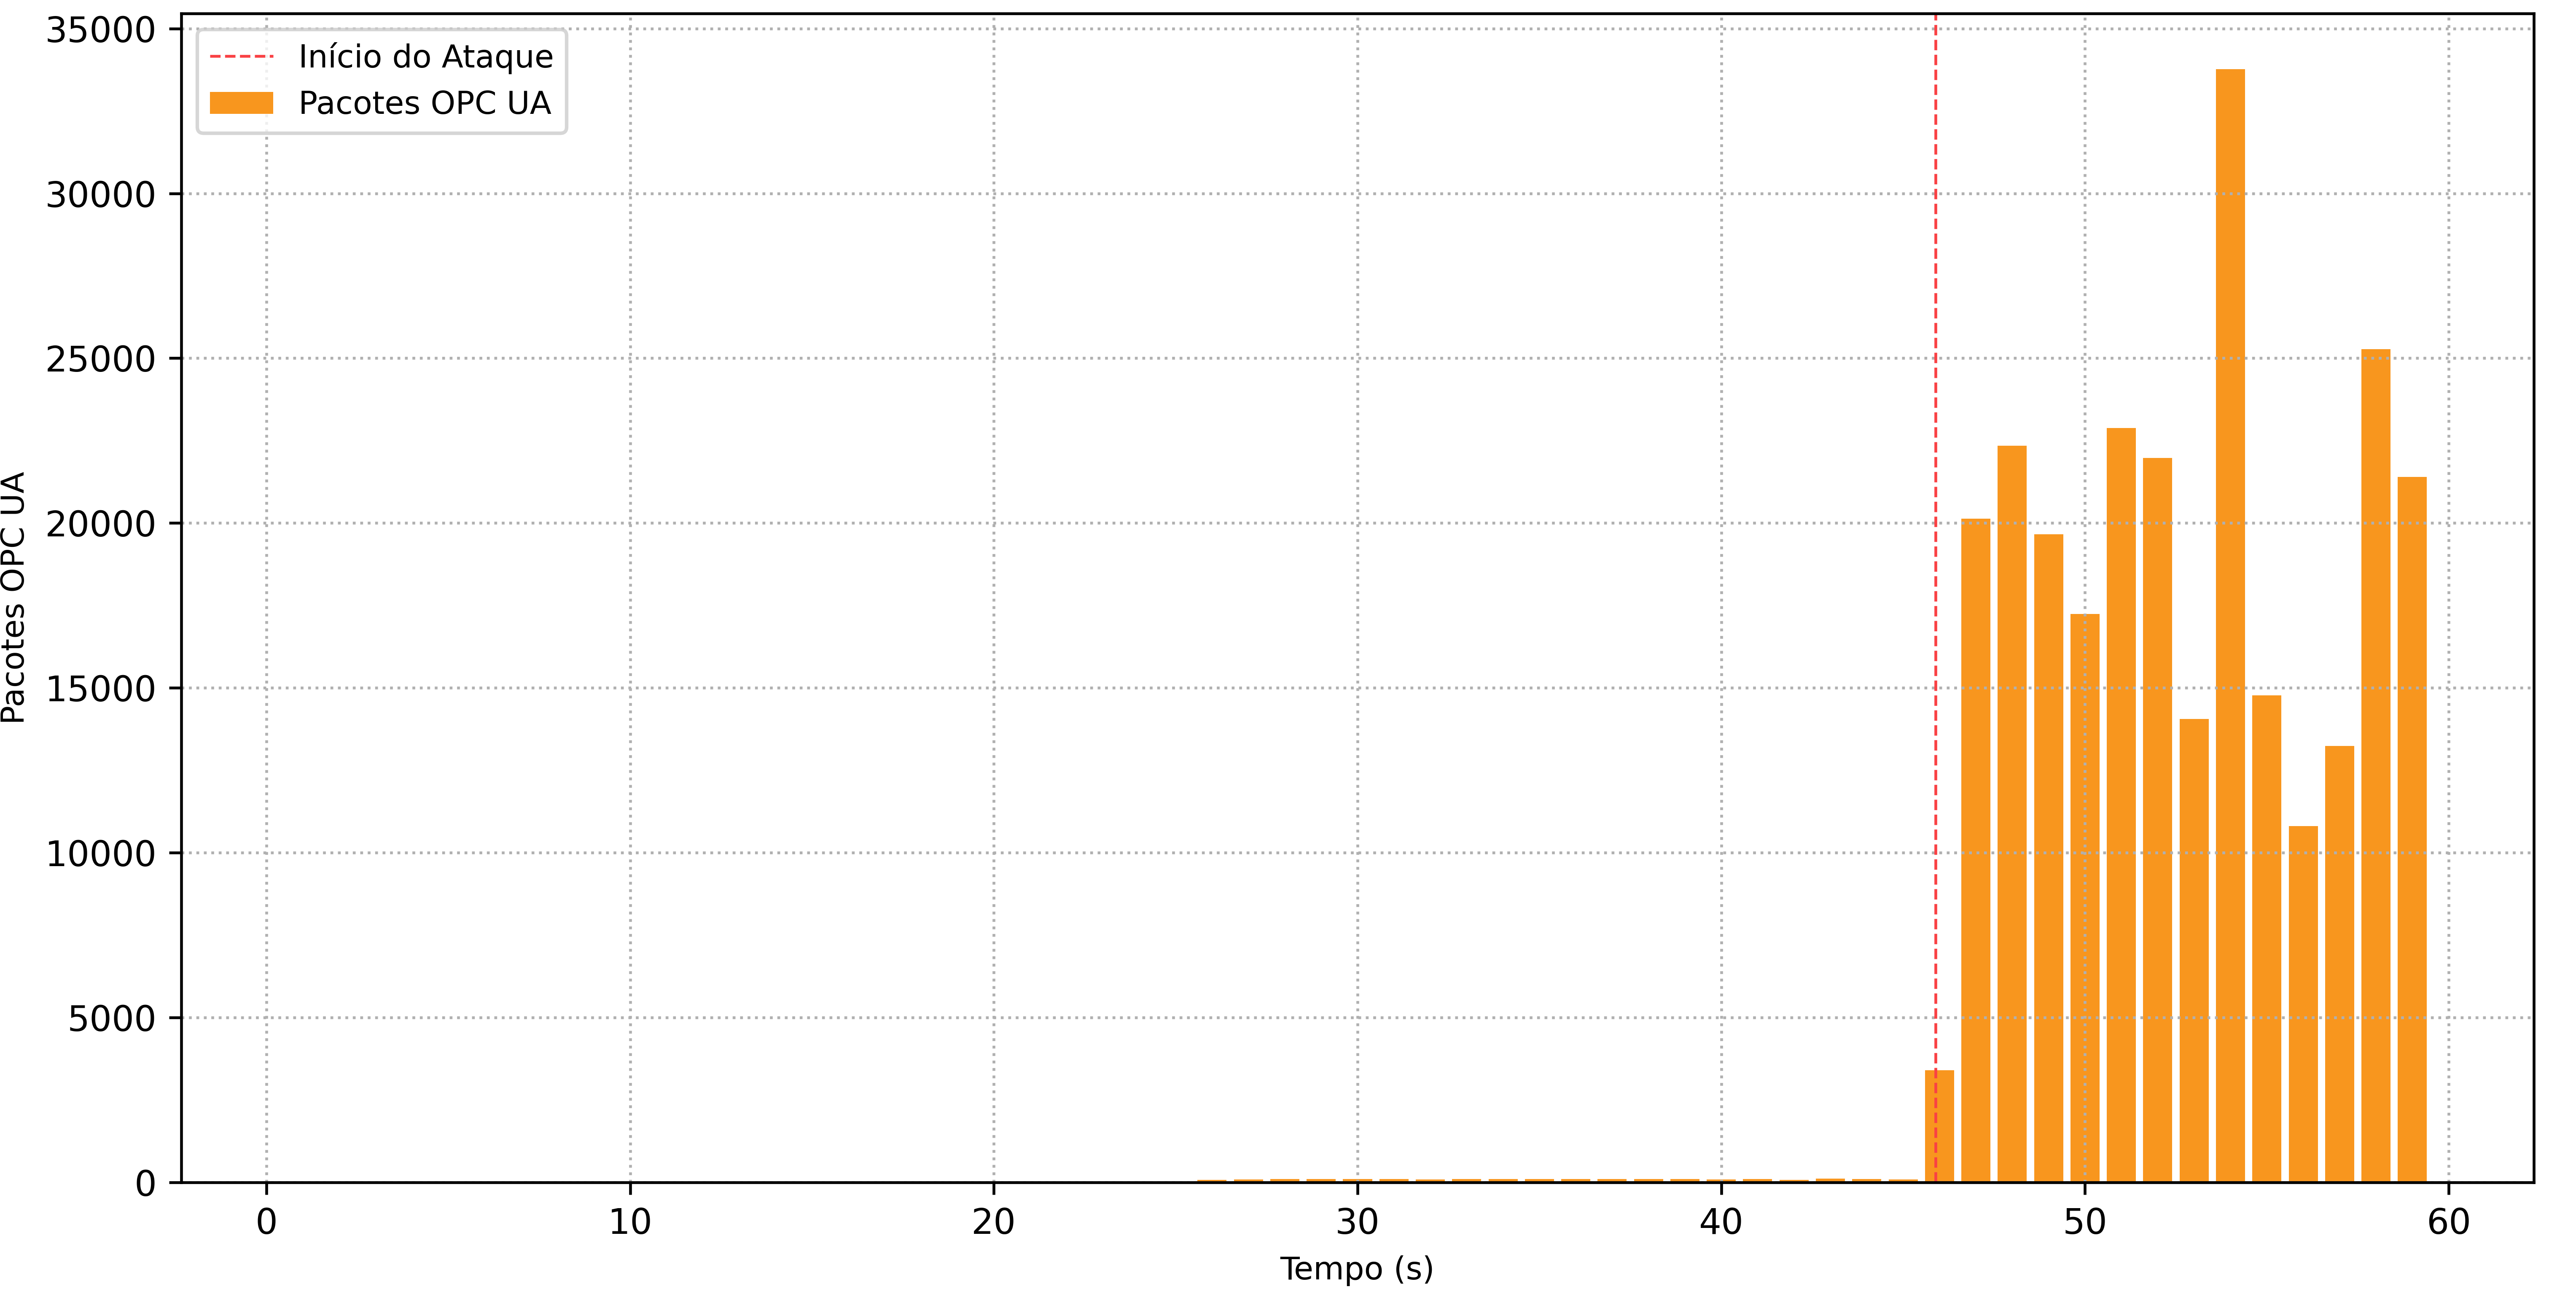
\includegraphics[width=1\textwidth, height=120pt]{USPSC-img/output/cropped/1-dos_hping3-pack.png}
    \end{subfigure}%
    ~
    \begin{subfigure}[t]{0.5\textwidth}
        \centering
        \caption{RTT por pacote}
        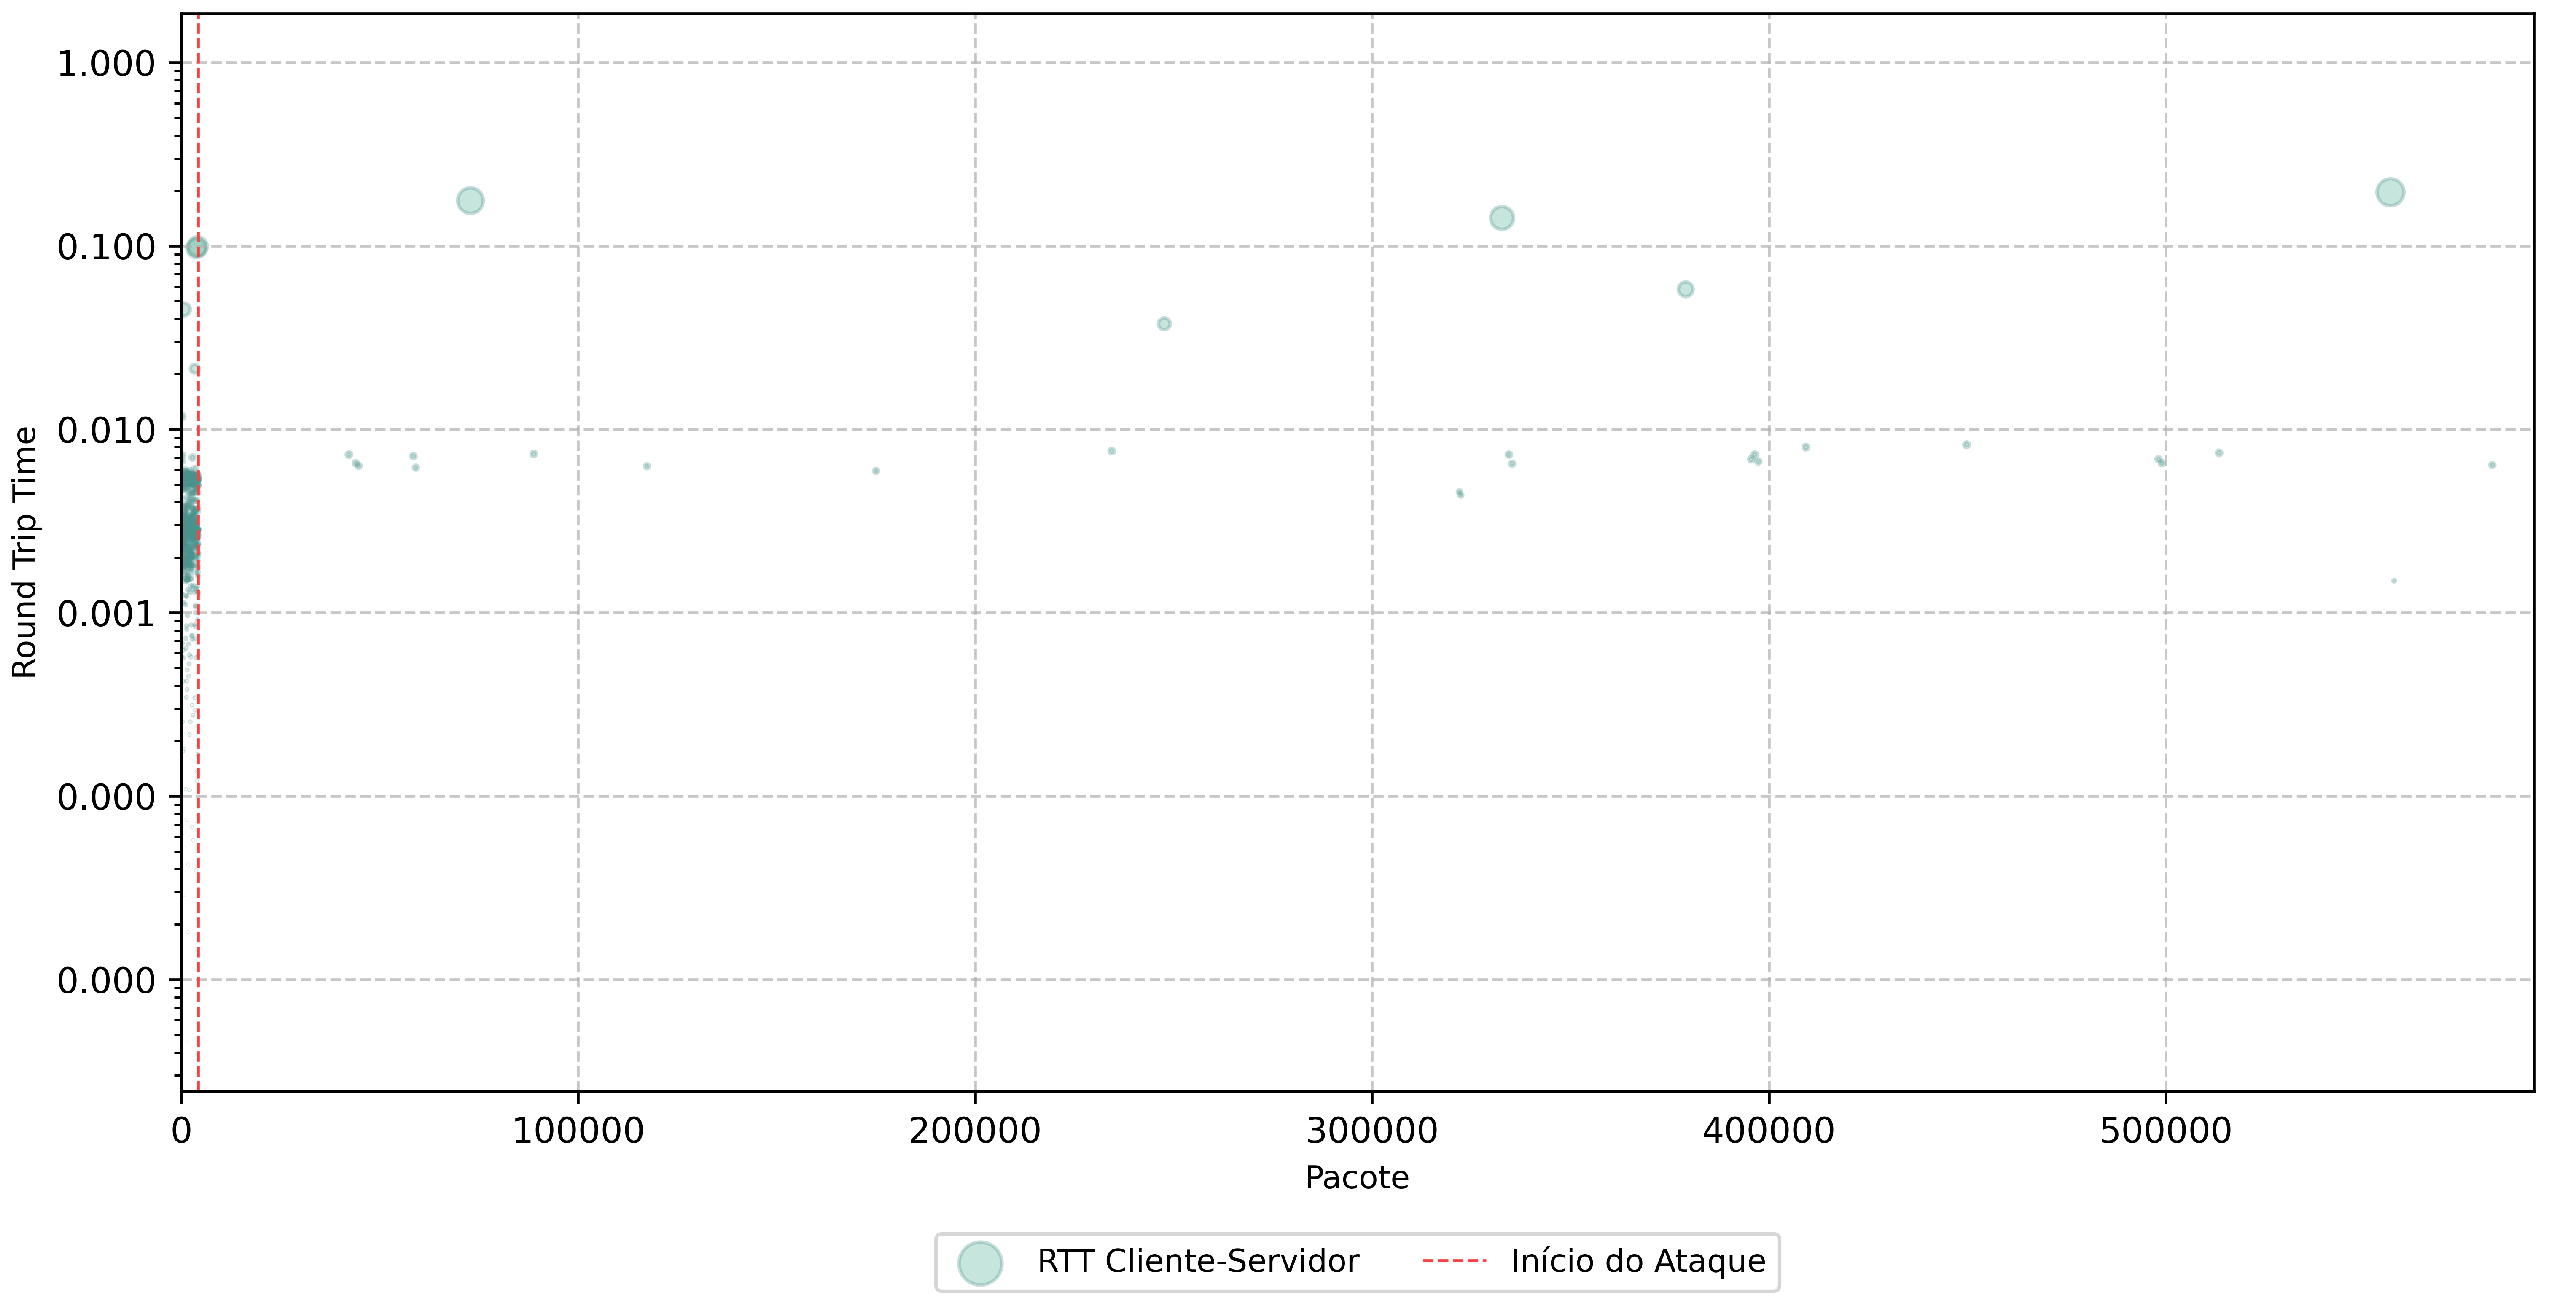
\includegraphics[width=1\textwidth, height=120pt]{USPSC-img/output/cropped/1-dos_hping3-rttp.png}
    \end{subfigure}%
    % ~
    % \begin{subfigure}[t]{0.5\textwidth}
    %     \centering
    %     \caption{RTT por segundos}
    %     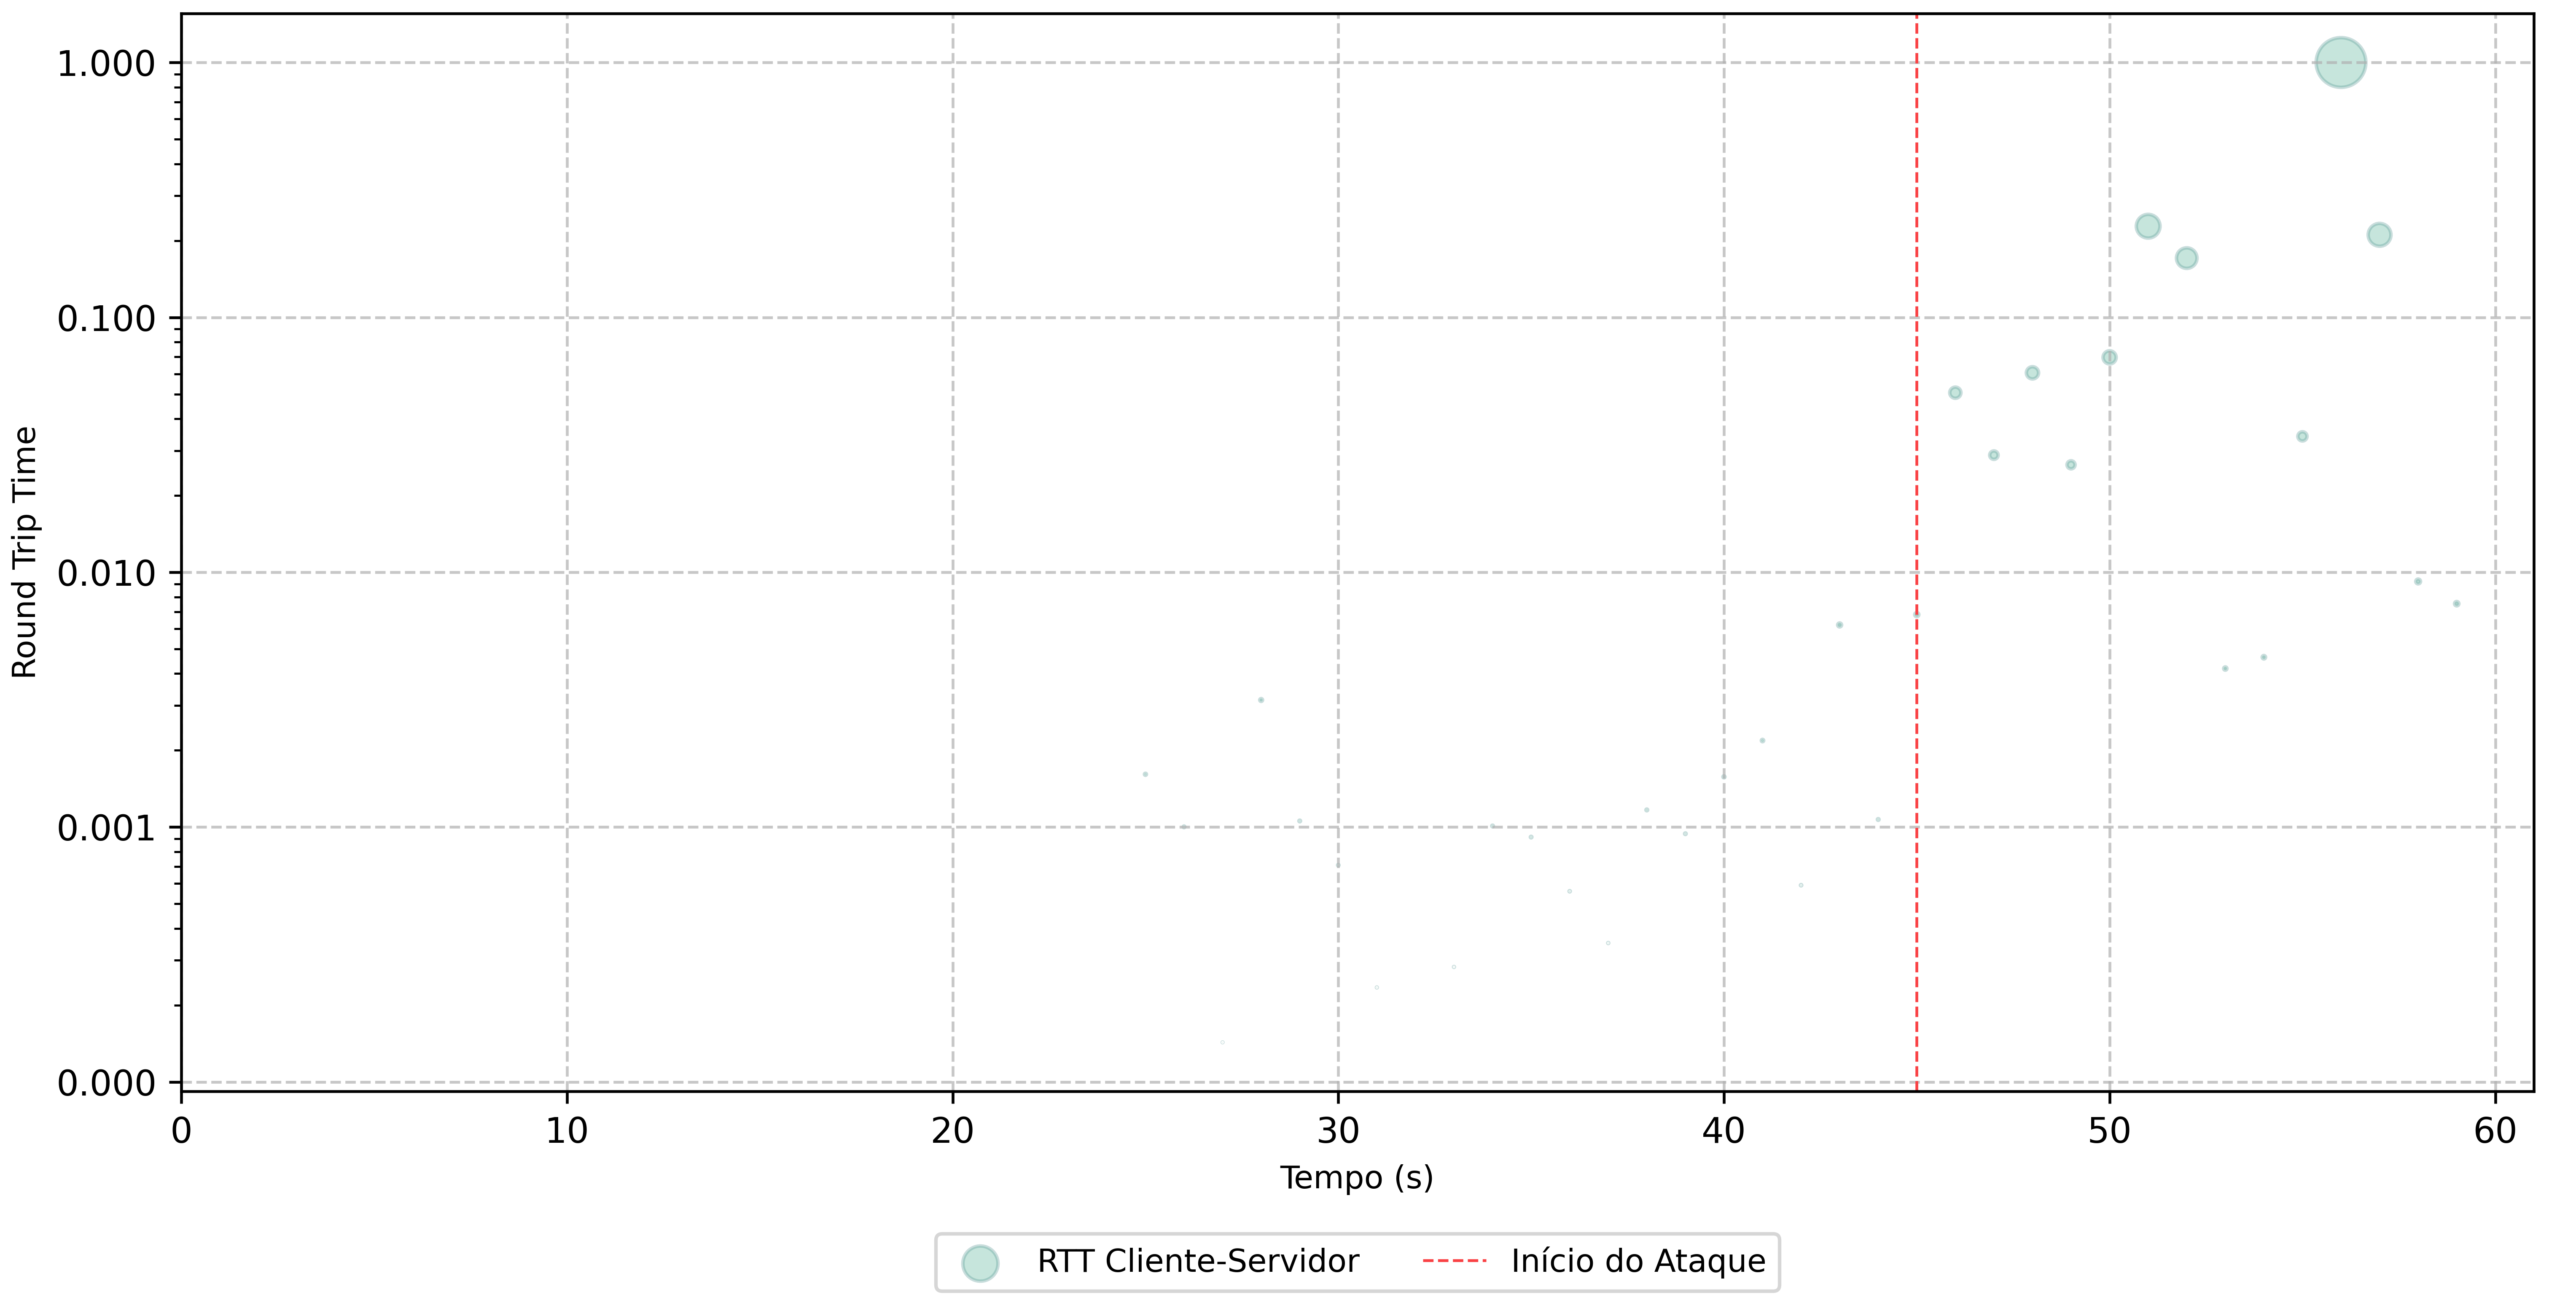
\includegraphics[width=1\textwidth, height=120pt]{USPSC-img/output/cropped/1-dos_hping3-rtts.png}
    % \end{subfigure}%
\end{figure}

\begin{figure}[htbp!]
    \centering
    \caption{\label{fig:2-dos_hping3}Gráficos do ataque de DoS por inundação TCP/IP - nível de segurança: `Sign \& Encrypt'.}
    \begin{subfigure}[t]{0.5\textwidth}
        \centering
        \caption{\textit{Throughput}}
        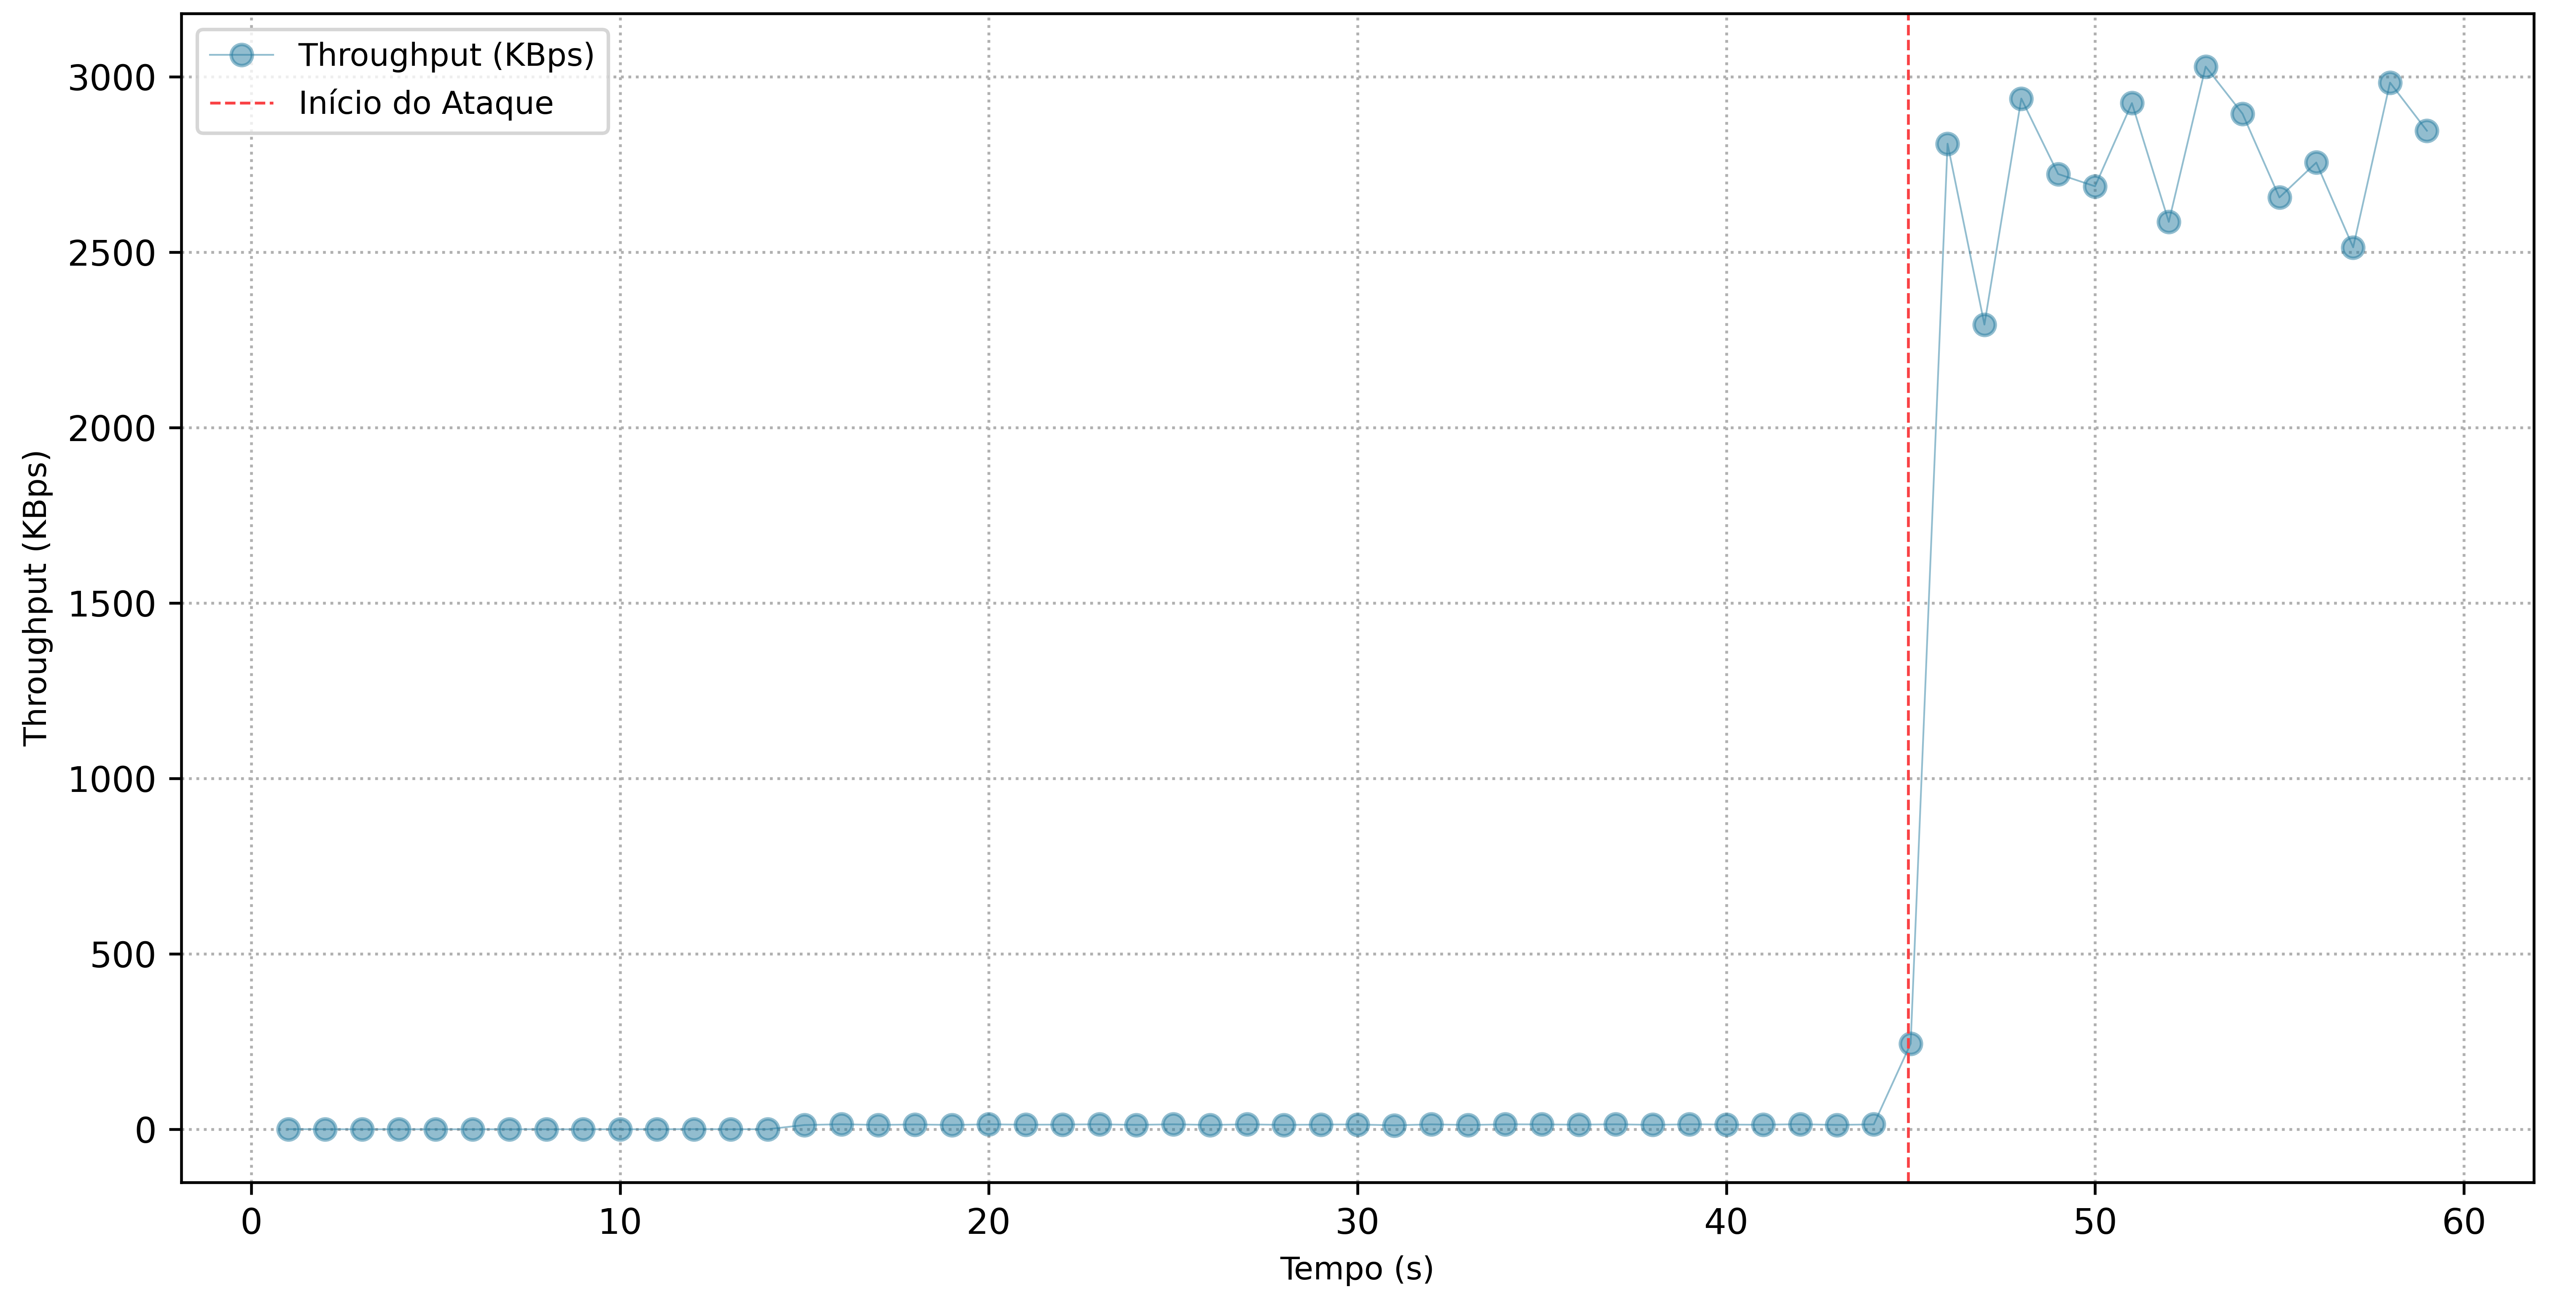
\includegraphics[width=1\textwidth, height=120pt]{USPSC-img/output/cropped/2-dos_hping3-tput.png}
    \end{subfigure}%
    ~ 
    \begin{subfigure}[t]{0.5\textwidth}
        \centering
        \caption{Desempenho}
        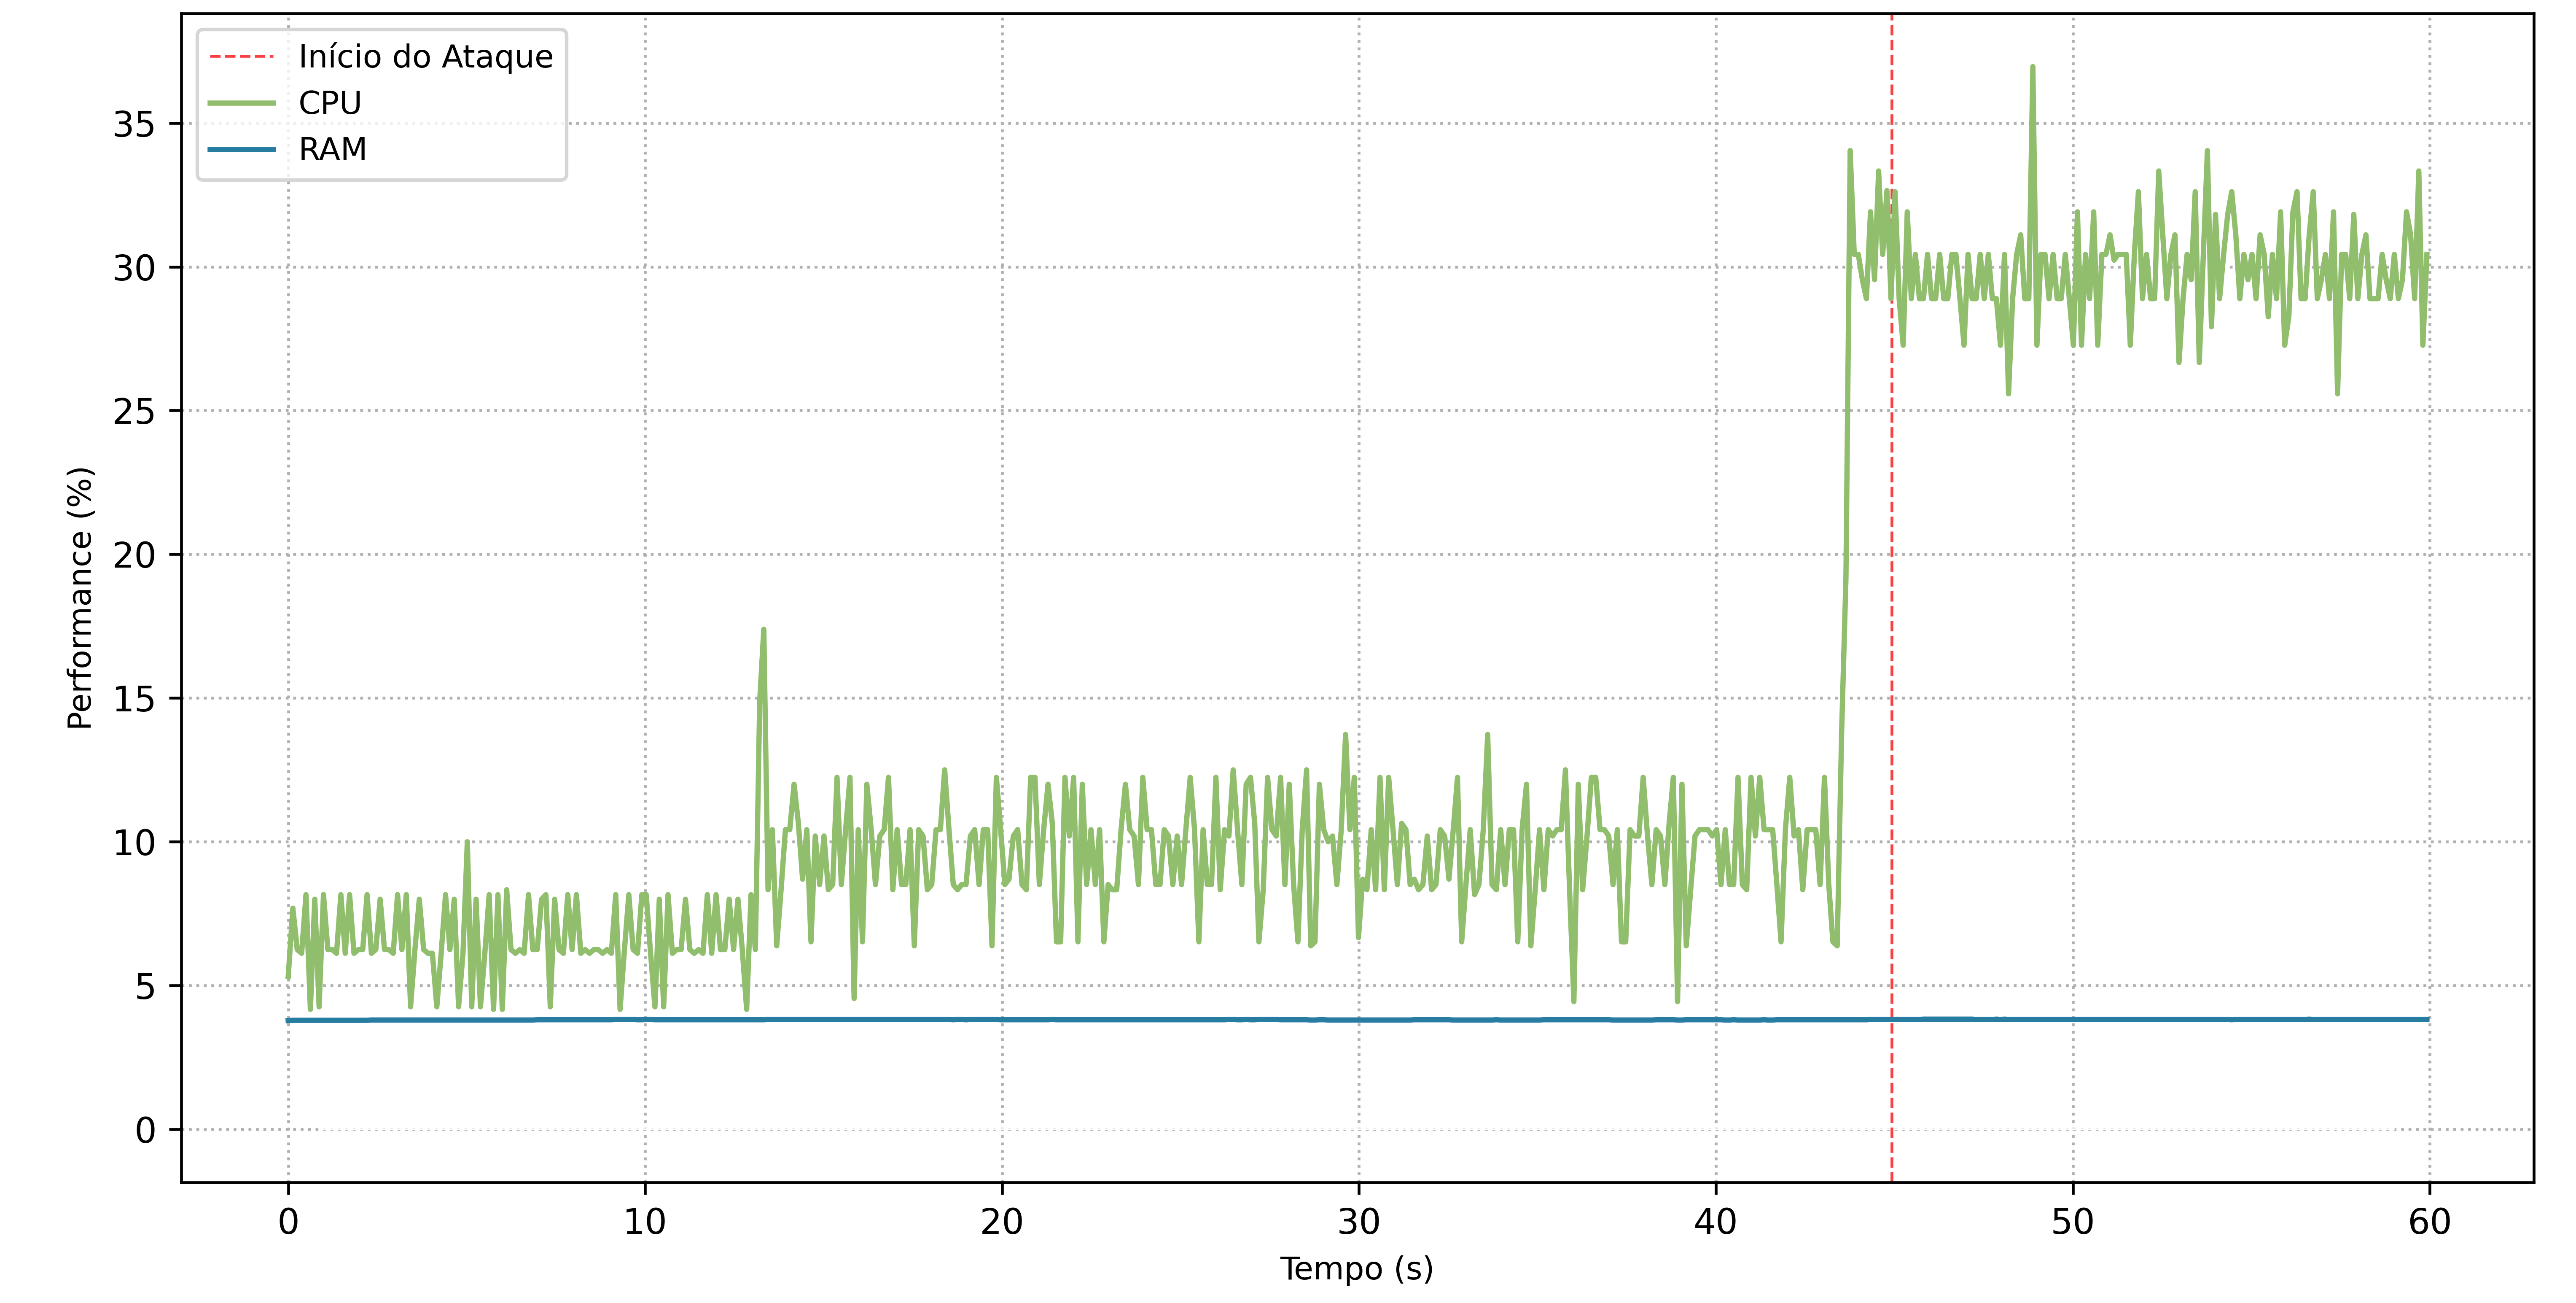
\includegraphics[width=1\textwidth, height=120pt]{USPSC-img/output/cropped/2-dos_hping3-perf.png}
    \end{subfigure}%
    \\
    % \begin{subfigure}[t]{0.5\textwidth}
    %     \centering
    %     \caption{Pacotes OPC UA}
    %     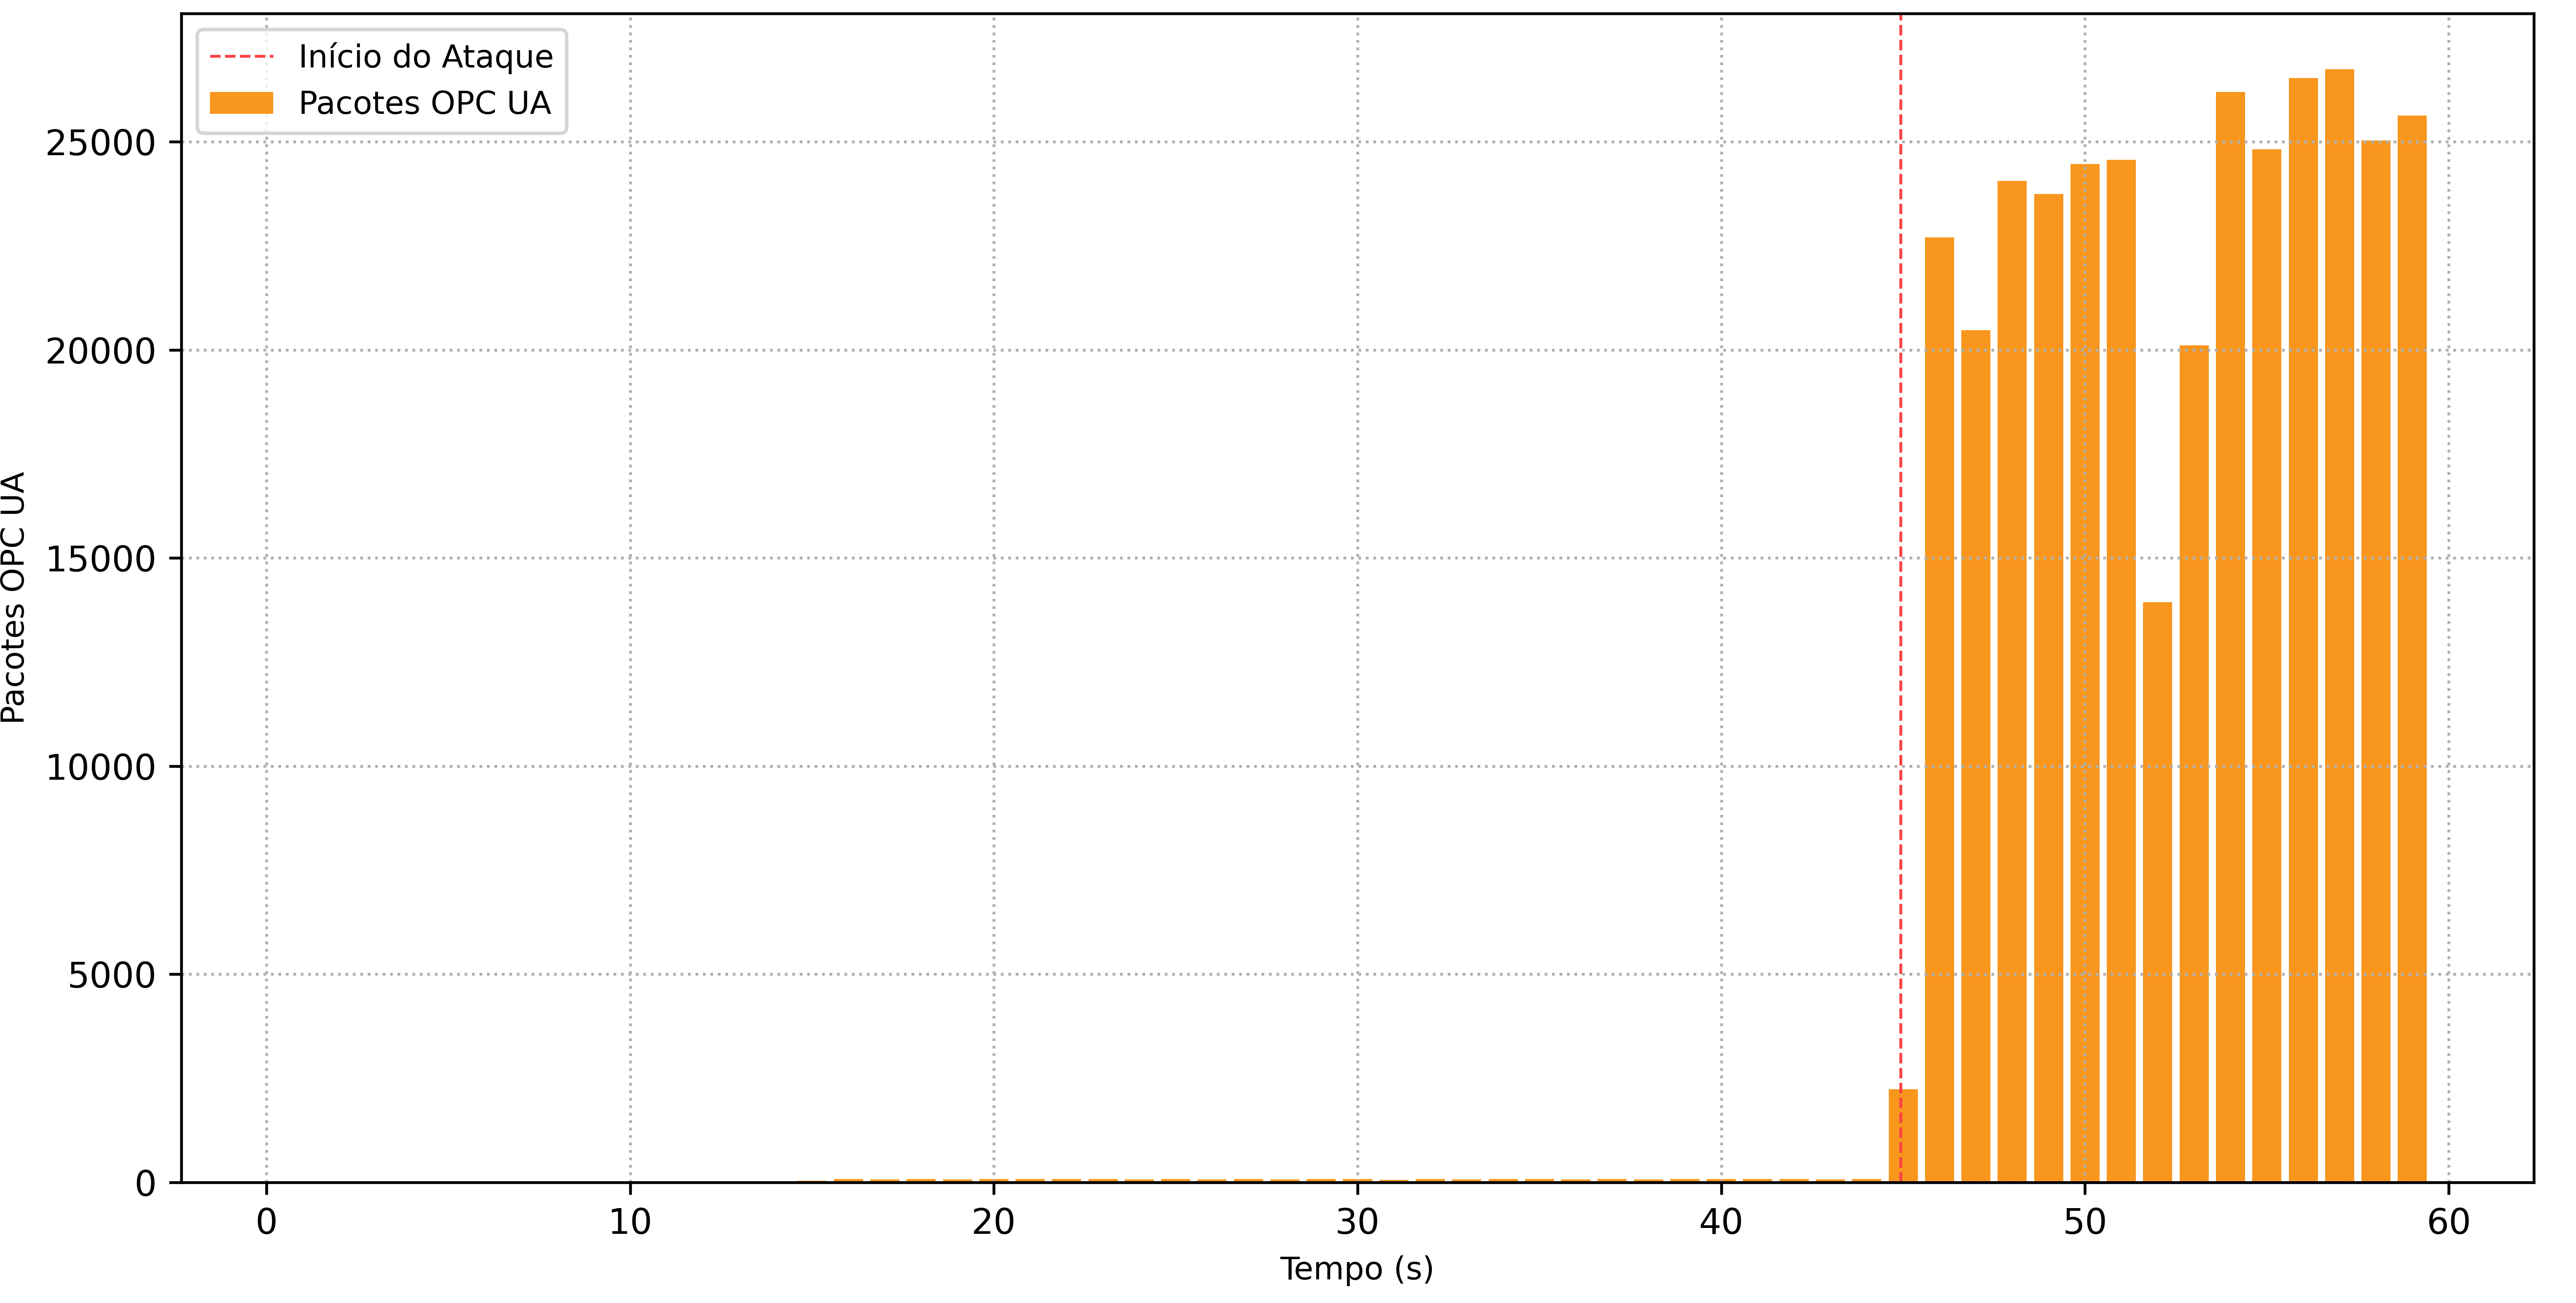
\includegraphics[width=1\textwidth, height=120pt]{USPSC-img/output/cropped/2-dos_hping3-pack.png}
    % \end{subfigure}%
    % ~
    \begin{subfigure}[t]{0.5\textwidth}
        \centering
        \caption{RTT por pacote}
        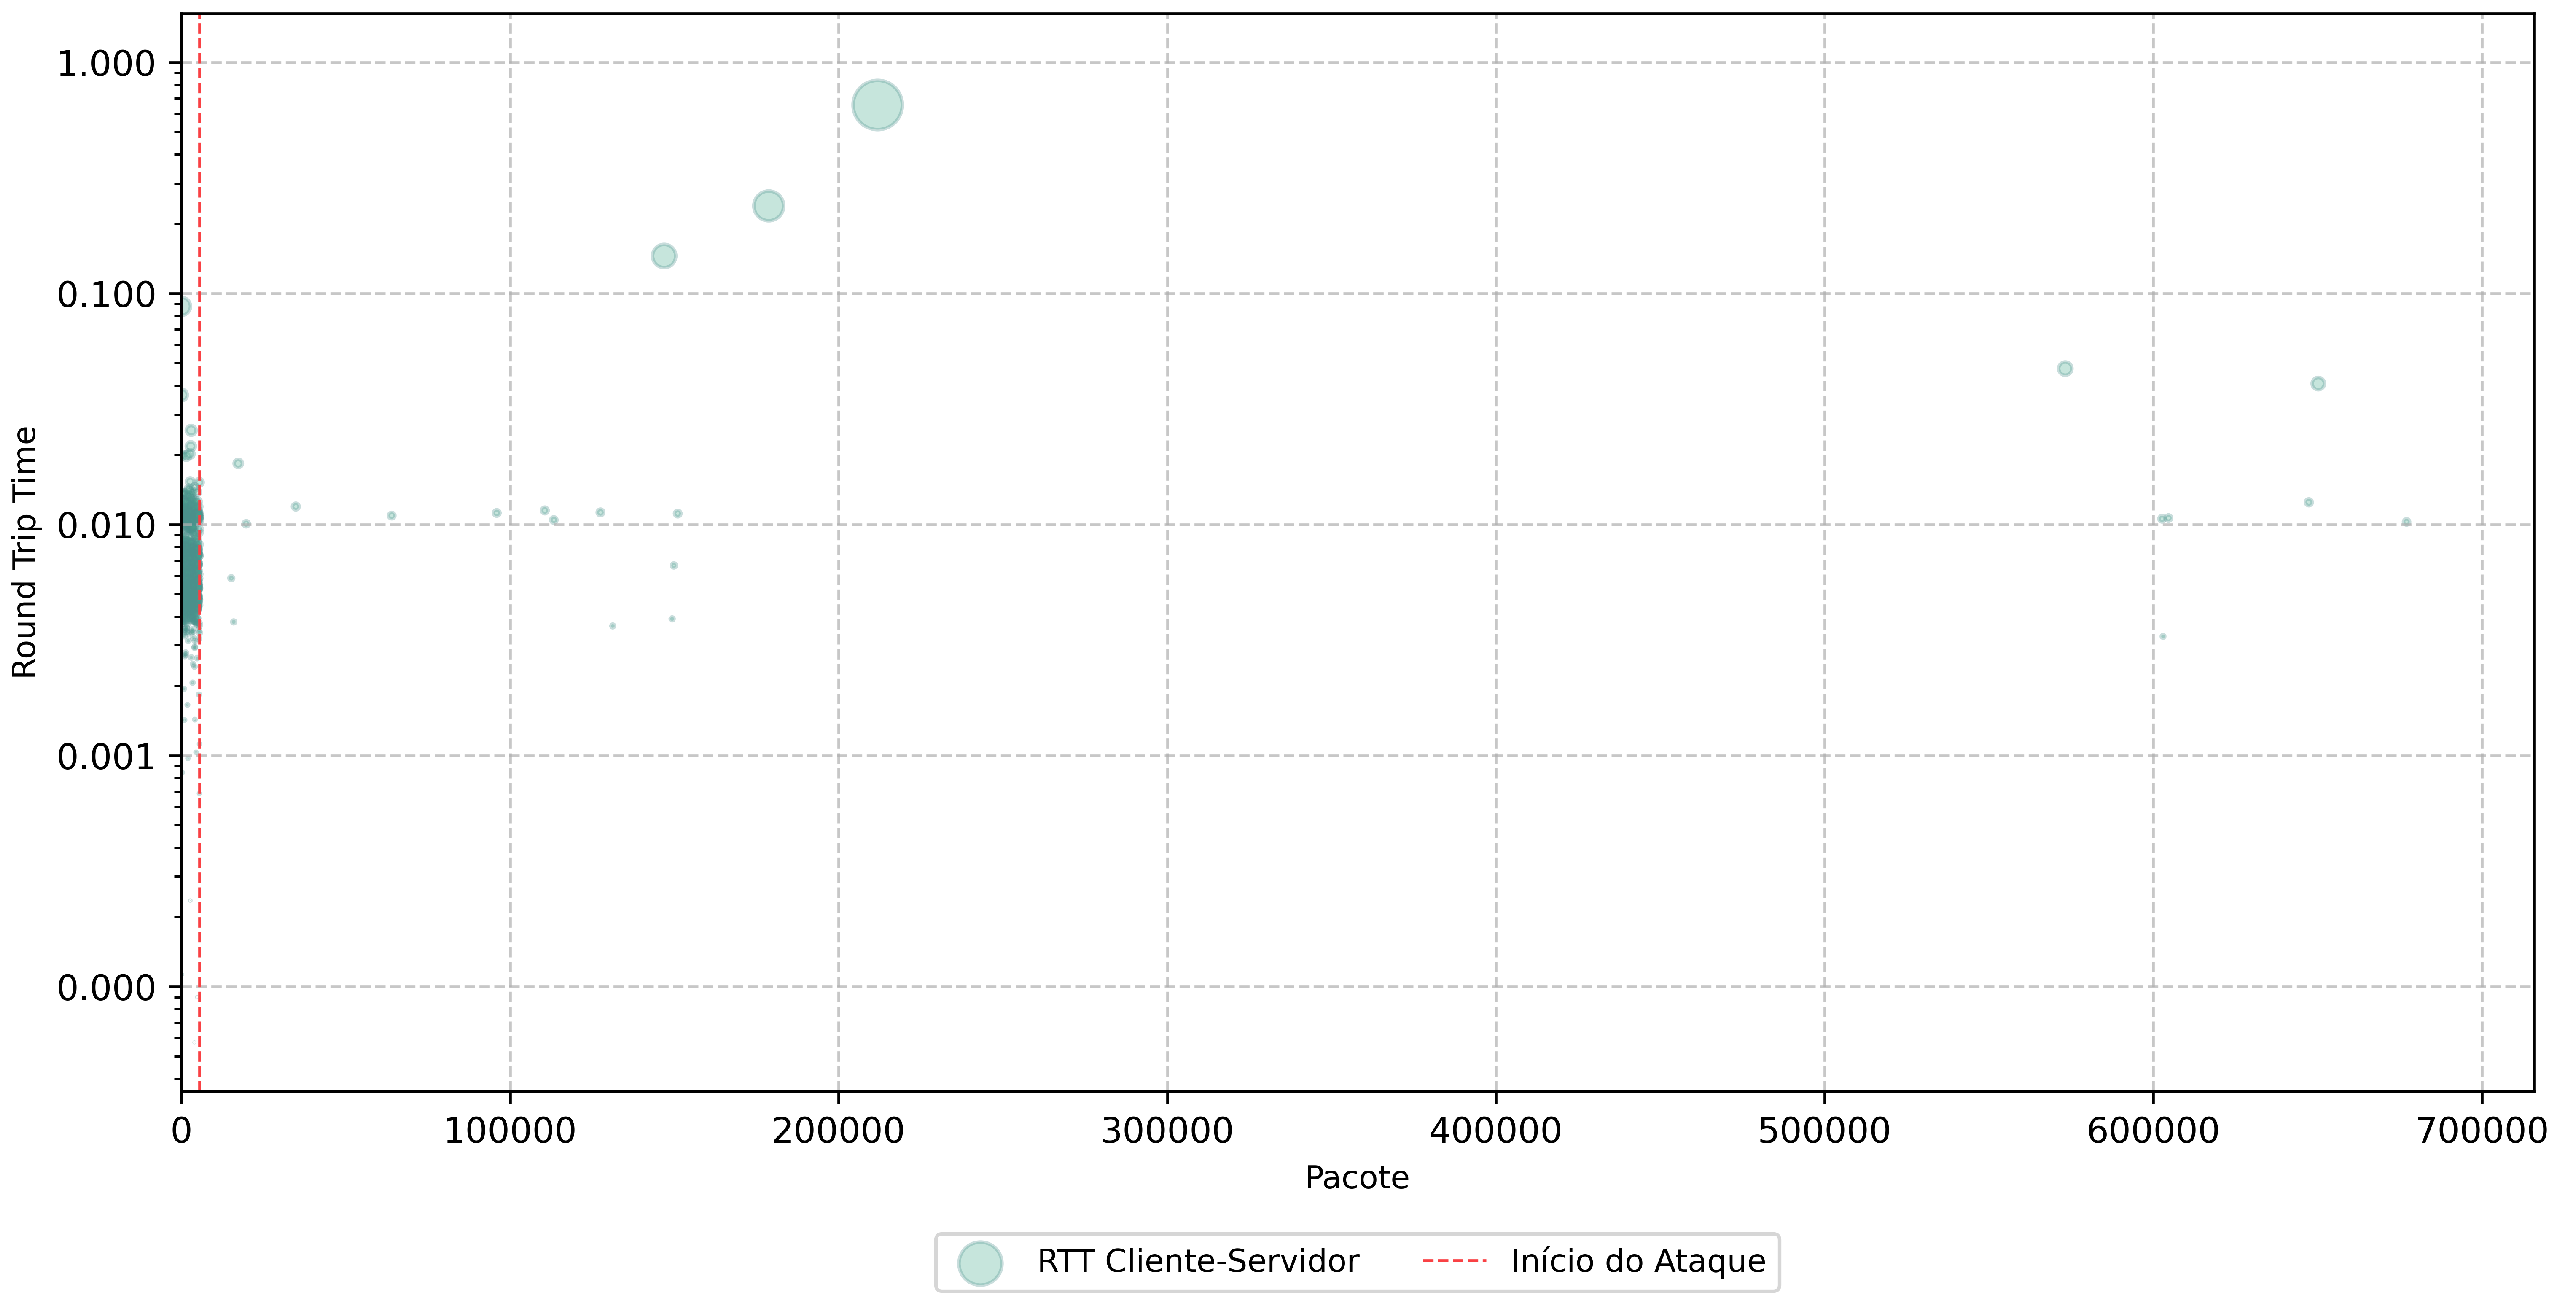
\includegraphics[width=1\textwidth, height=120pt]{USPSC-img/output/cropped/2-dos_hping3-rttp.png}
    \end{subfigure}%
    ~
    \begin{subfigure}[t]{0.5\textwidth}
        \centering
        \caption{RTT por segundos}
        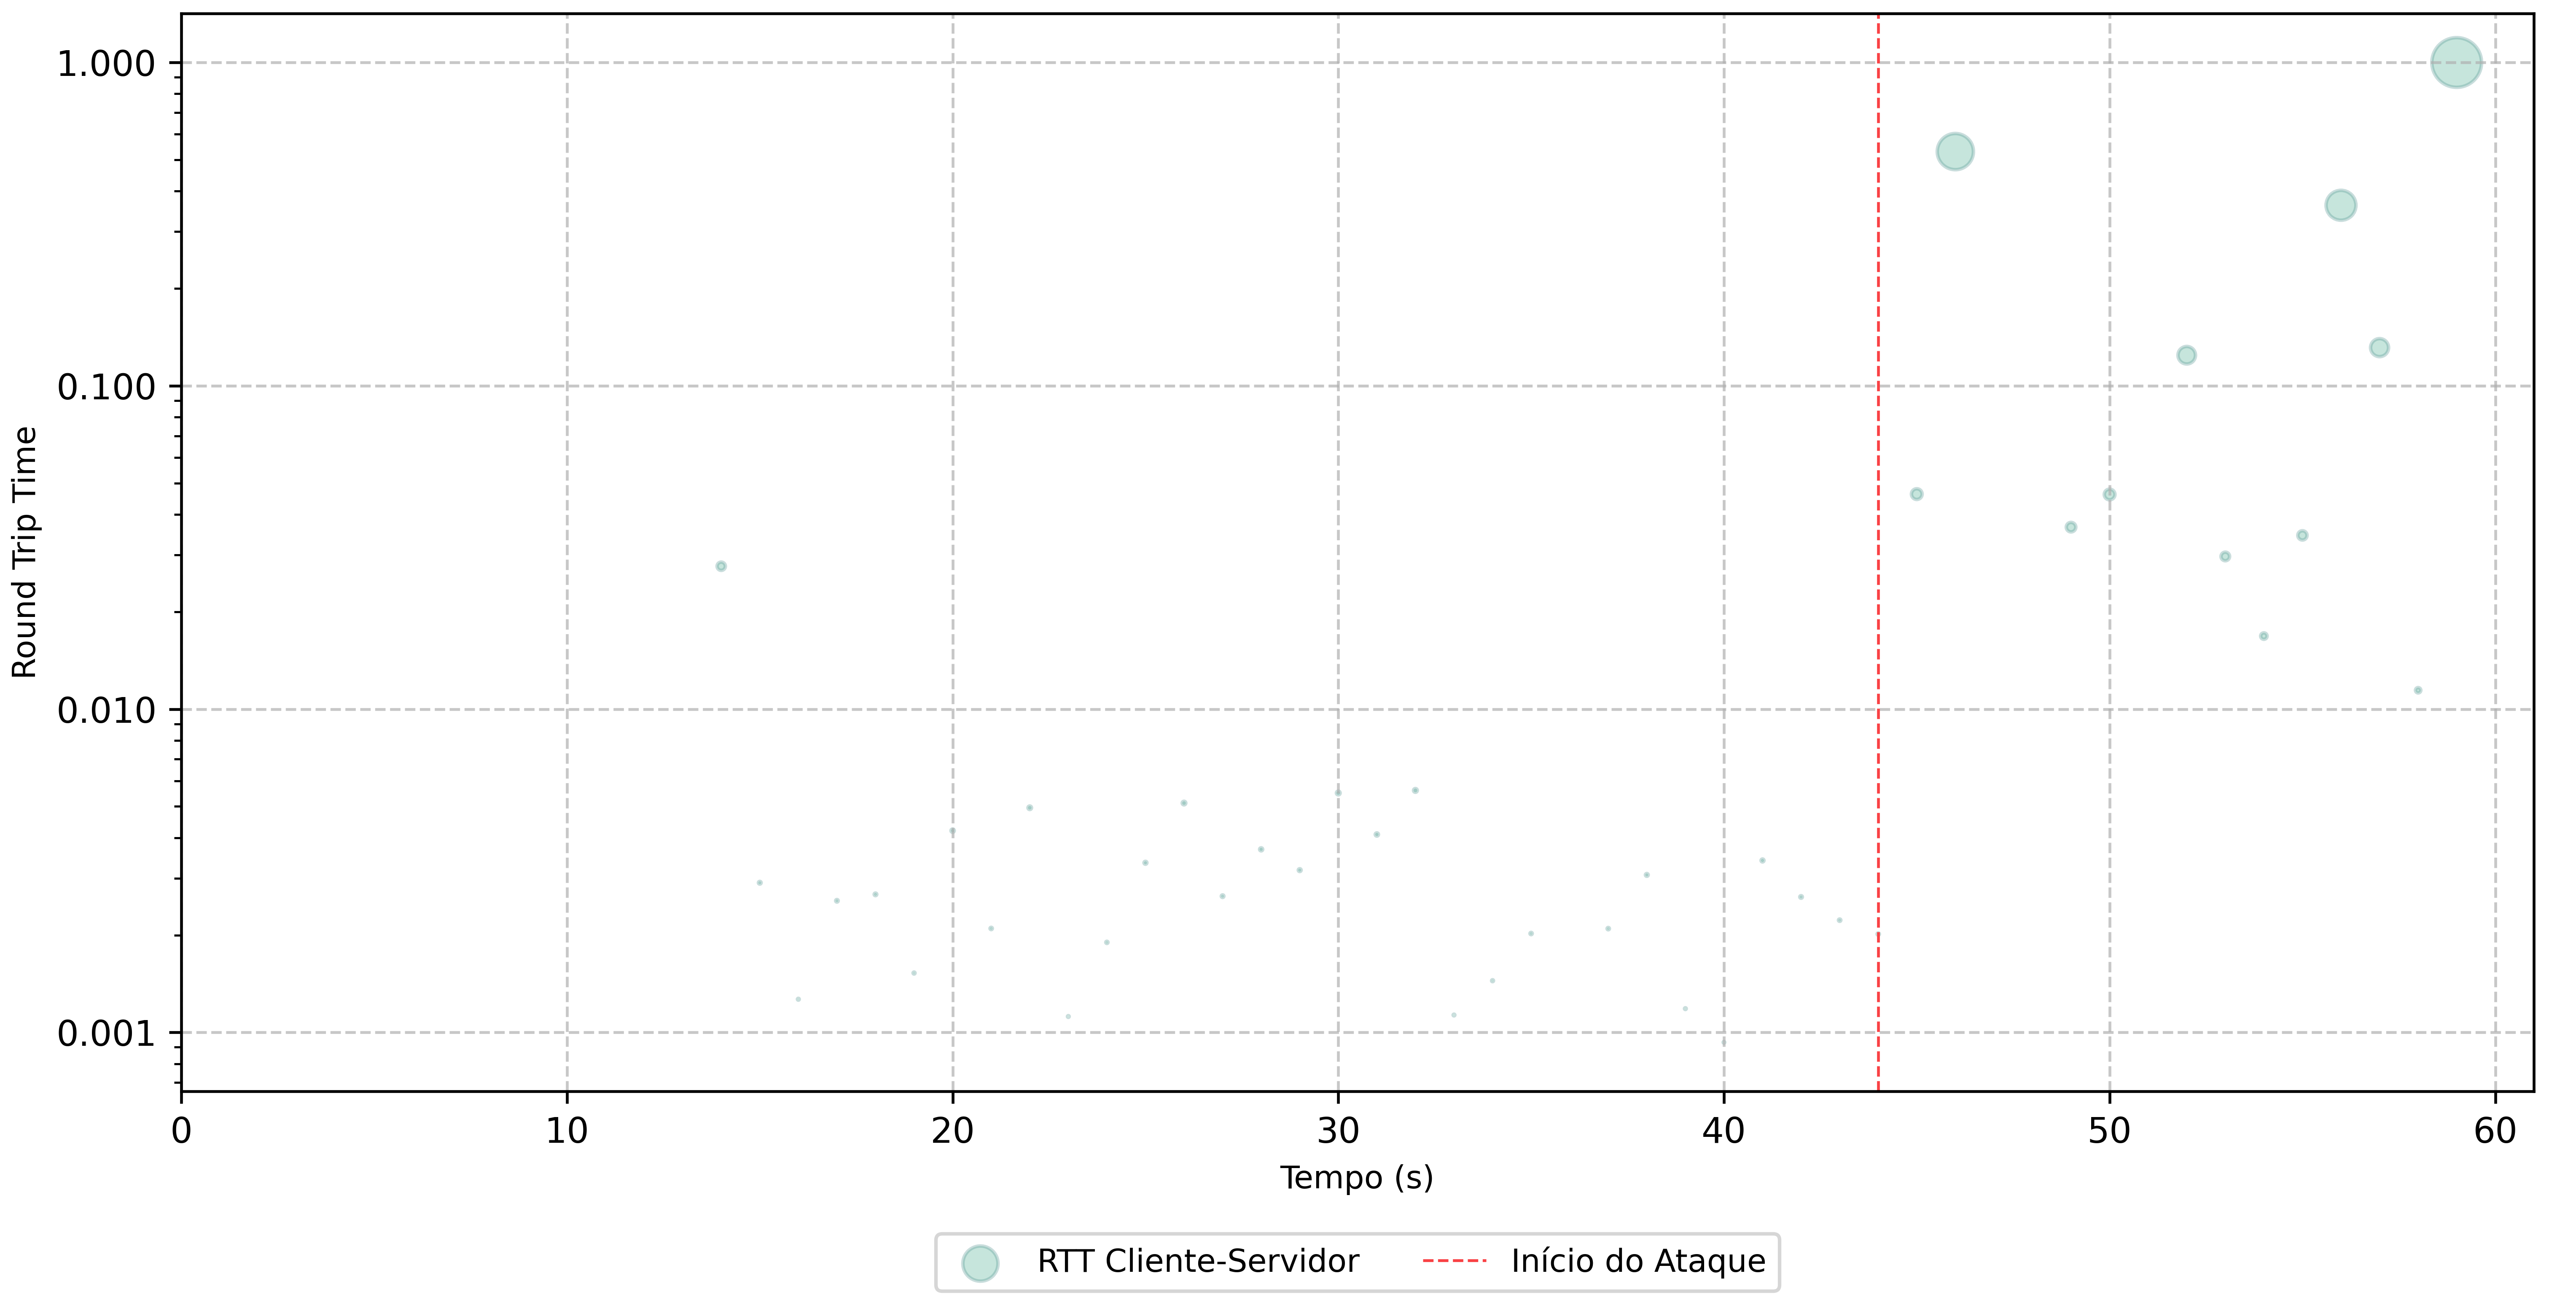
\includegraphics[width=1\textwidth, height=120pt]{USPSC-img/output/cropped/2-dos_hping3-rtts.png}
    \end{subfigure}%
\end{figure}

\begin{figure}[htbp!]
    \centering
    \caption{\label{fig:0-dos_open_multiple_secure_channels}Gráficos do ataque de DoS pela abertura de múltiplos canais seguros - nível de segurança: `None'.}
    \begin{subfigure}[t]{0.5\textwidth}
        \centering
        \caption{\textit{Throughput}}
        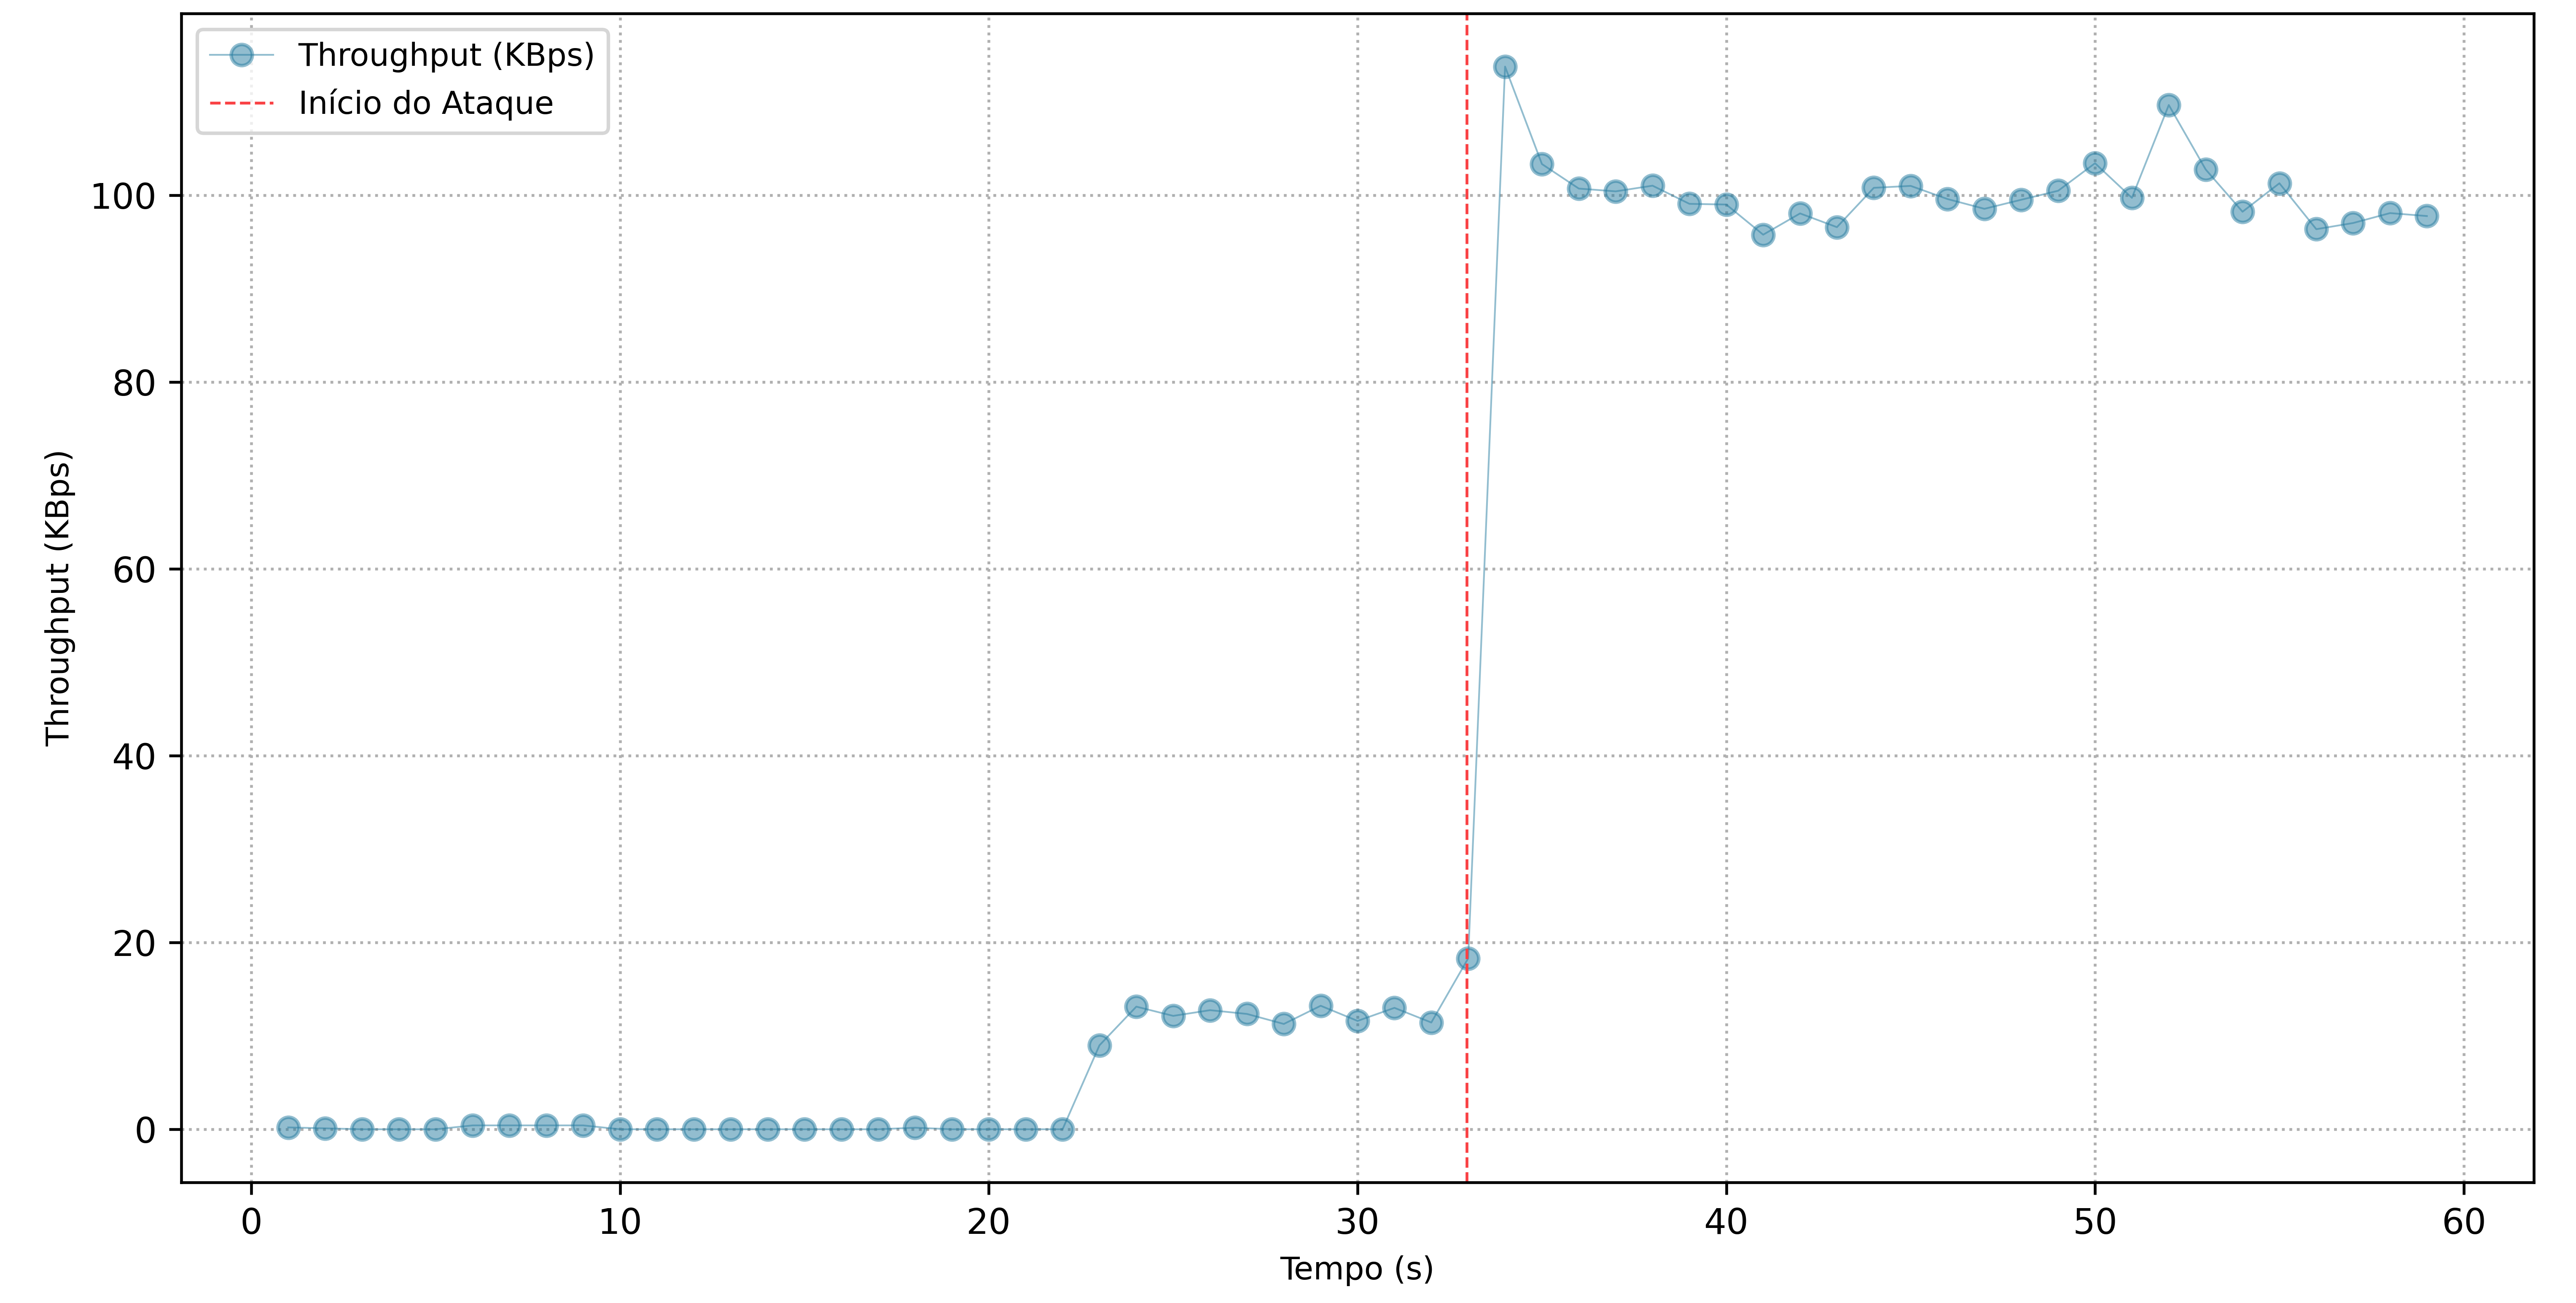
\includegraphics[width=1\textwidth, height=120pt]{USPSC-img/output/cropped/0-dos_open_multiple_secure_channels-tput.png}
    \end{subfigure}%
    ~ 
    \begin{subfigure}[t]{0.5\textwidth}
        \centering
        \caption{Desempenho}
        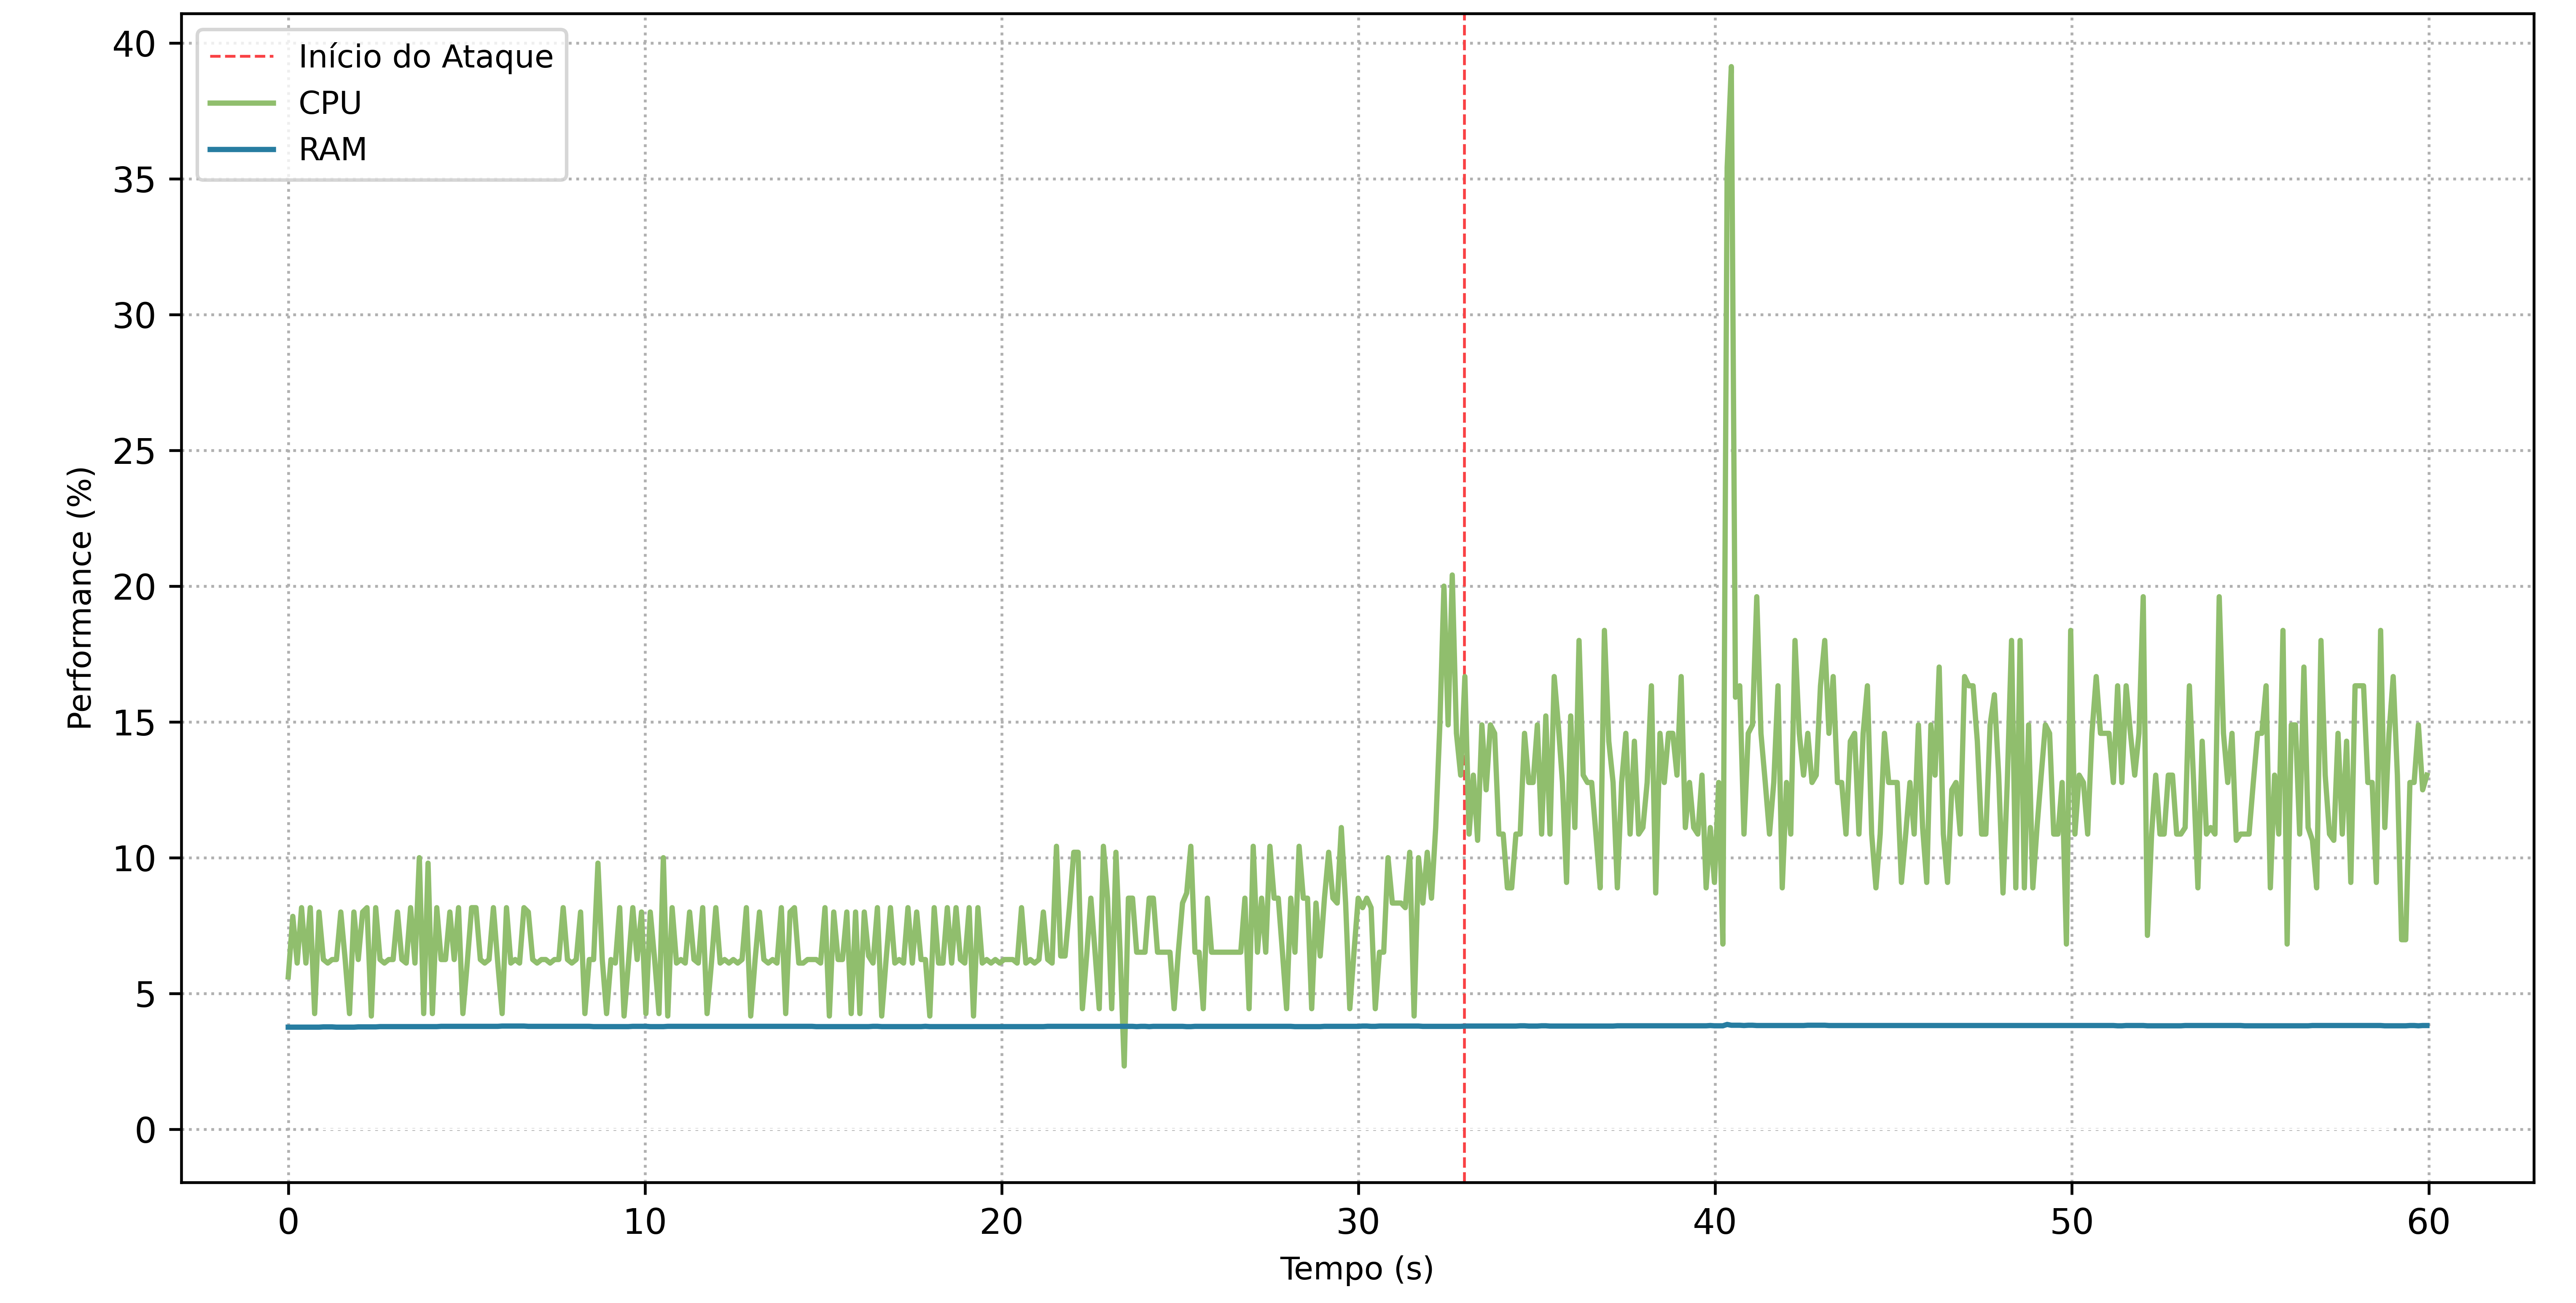
\includegraphics[width=1\textwidth, height=120pt]{USPSC-img/output/cropped/0-dos_open_multiple_secure_channels-perf.png}
    \end{subfigure}%
    \\
    \begin{subfigure}[t]{0.5\textwidth}
        \centering
        \caption{Pacotes OPC UA}
        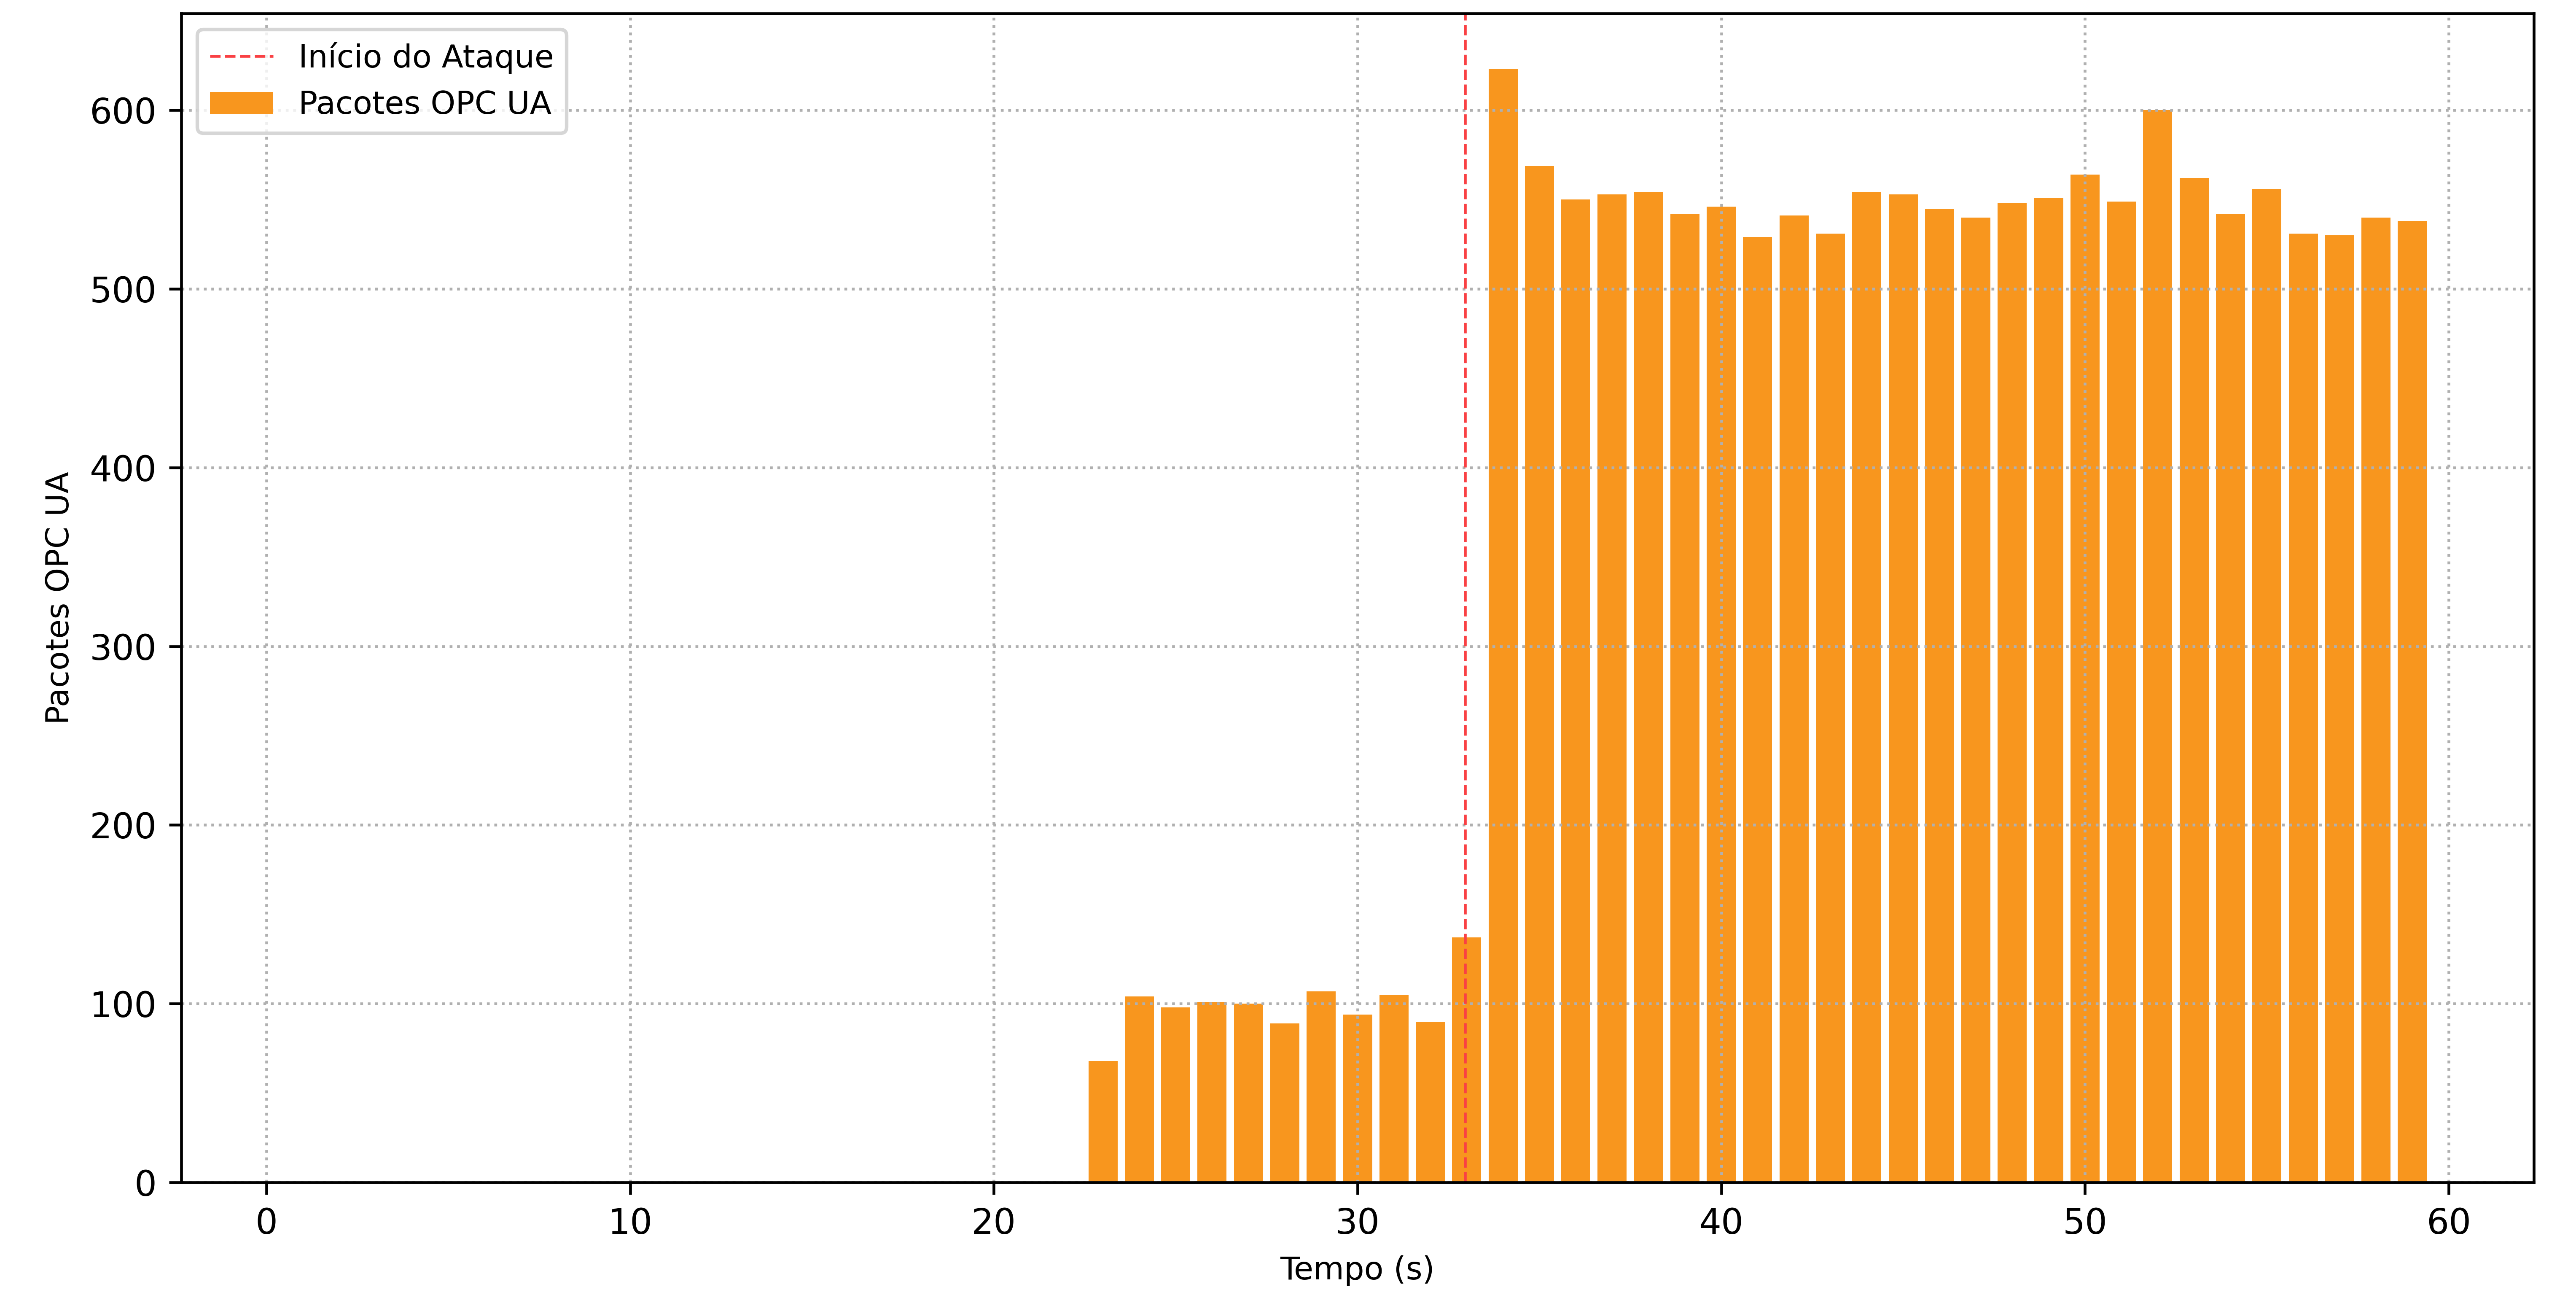
\includegraphics[width=1\textwidth, height=120pt]{USPSC-img/output/cropped/0-dos_open_multiple_secure_channels-pack.png}
    \end{subfigure}%
    ~
    \begin{subfigure}[t]{0.5\textwidth}
        \centering
        \caption{RTT por pacote}
        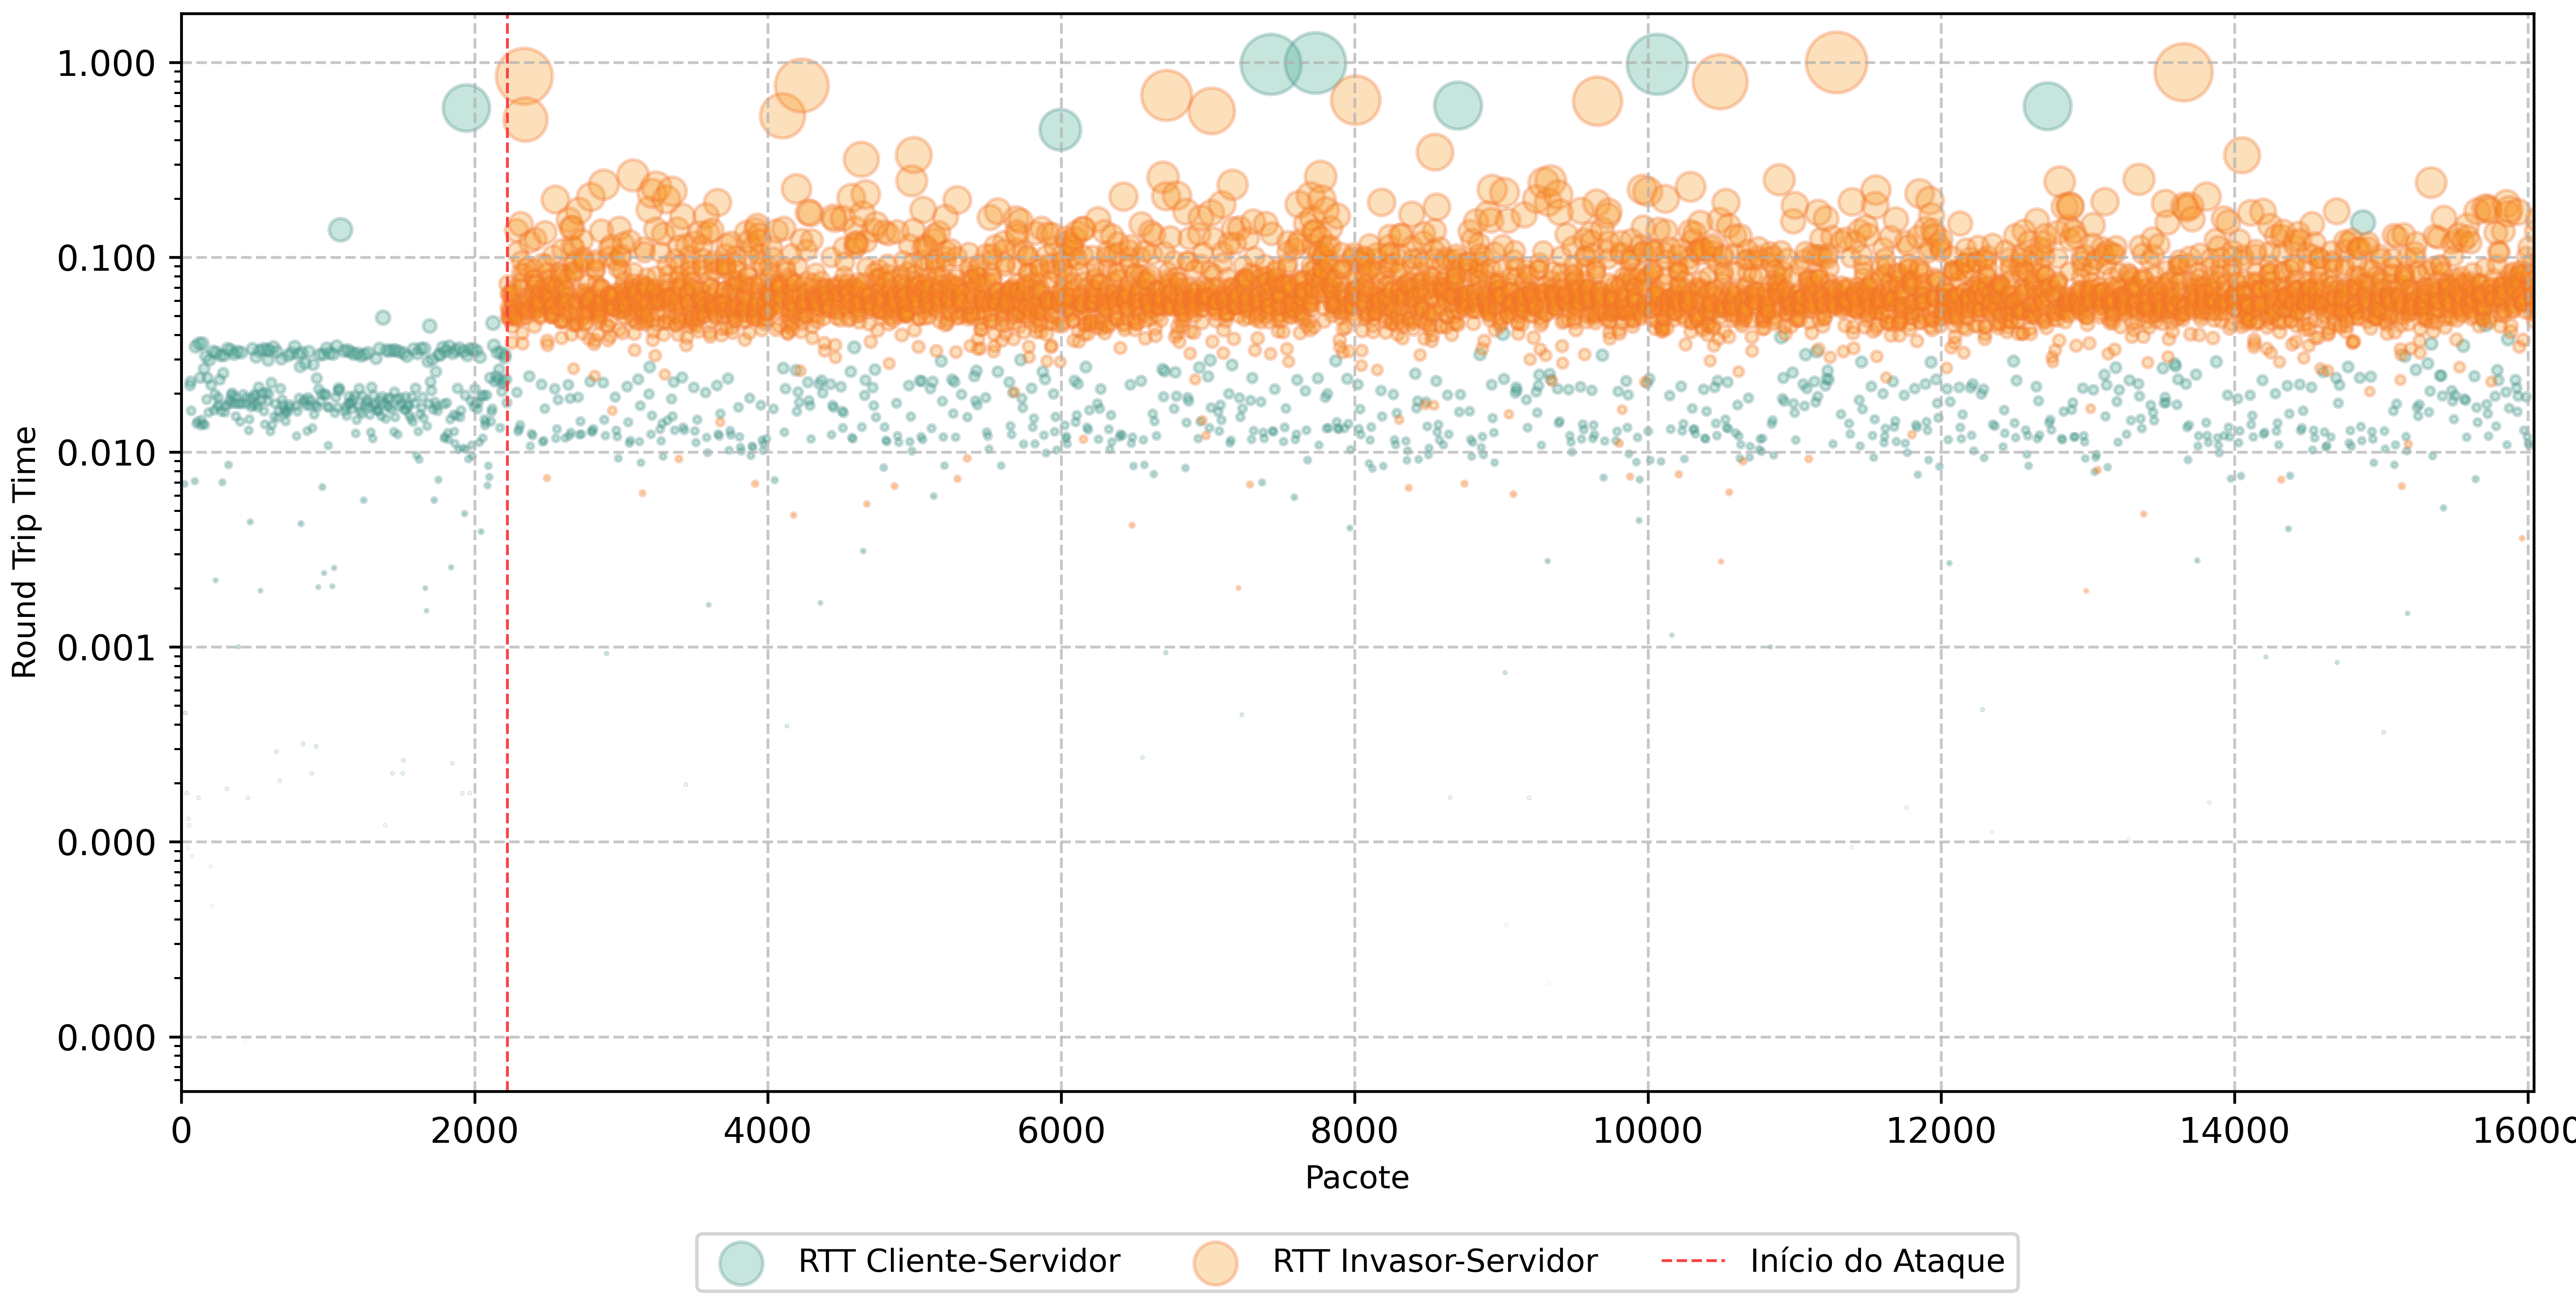
\includegraphics[width=1\textwidth, height=120pt]{USPSC-img/output/cropped/0-dos_open_multiple_secure_channels-rttp.png}
    \end{subfigure}%
    % ~
    % \begin{subfigure}[t]{0.5\textwidth}
    %     \centering
    %     \caption{RTT por segundos}
    %     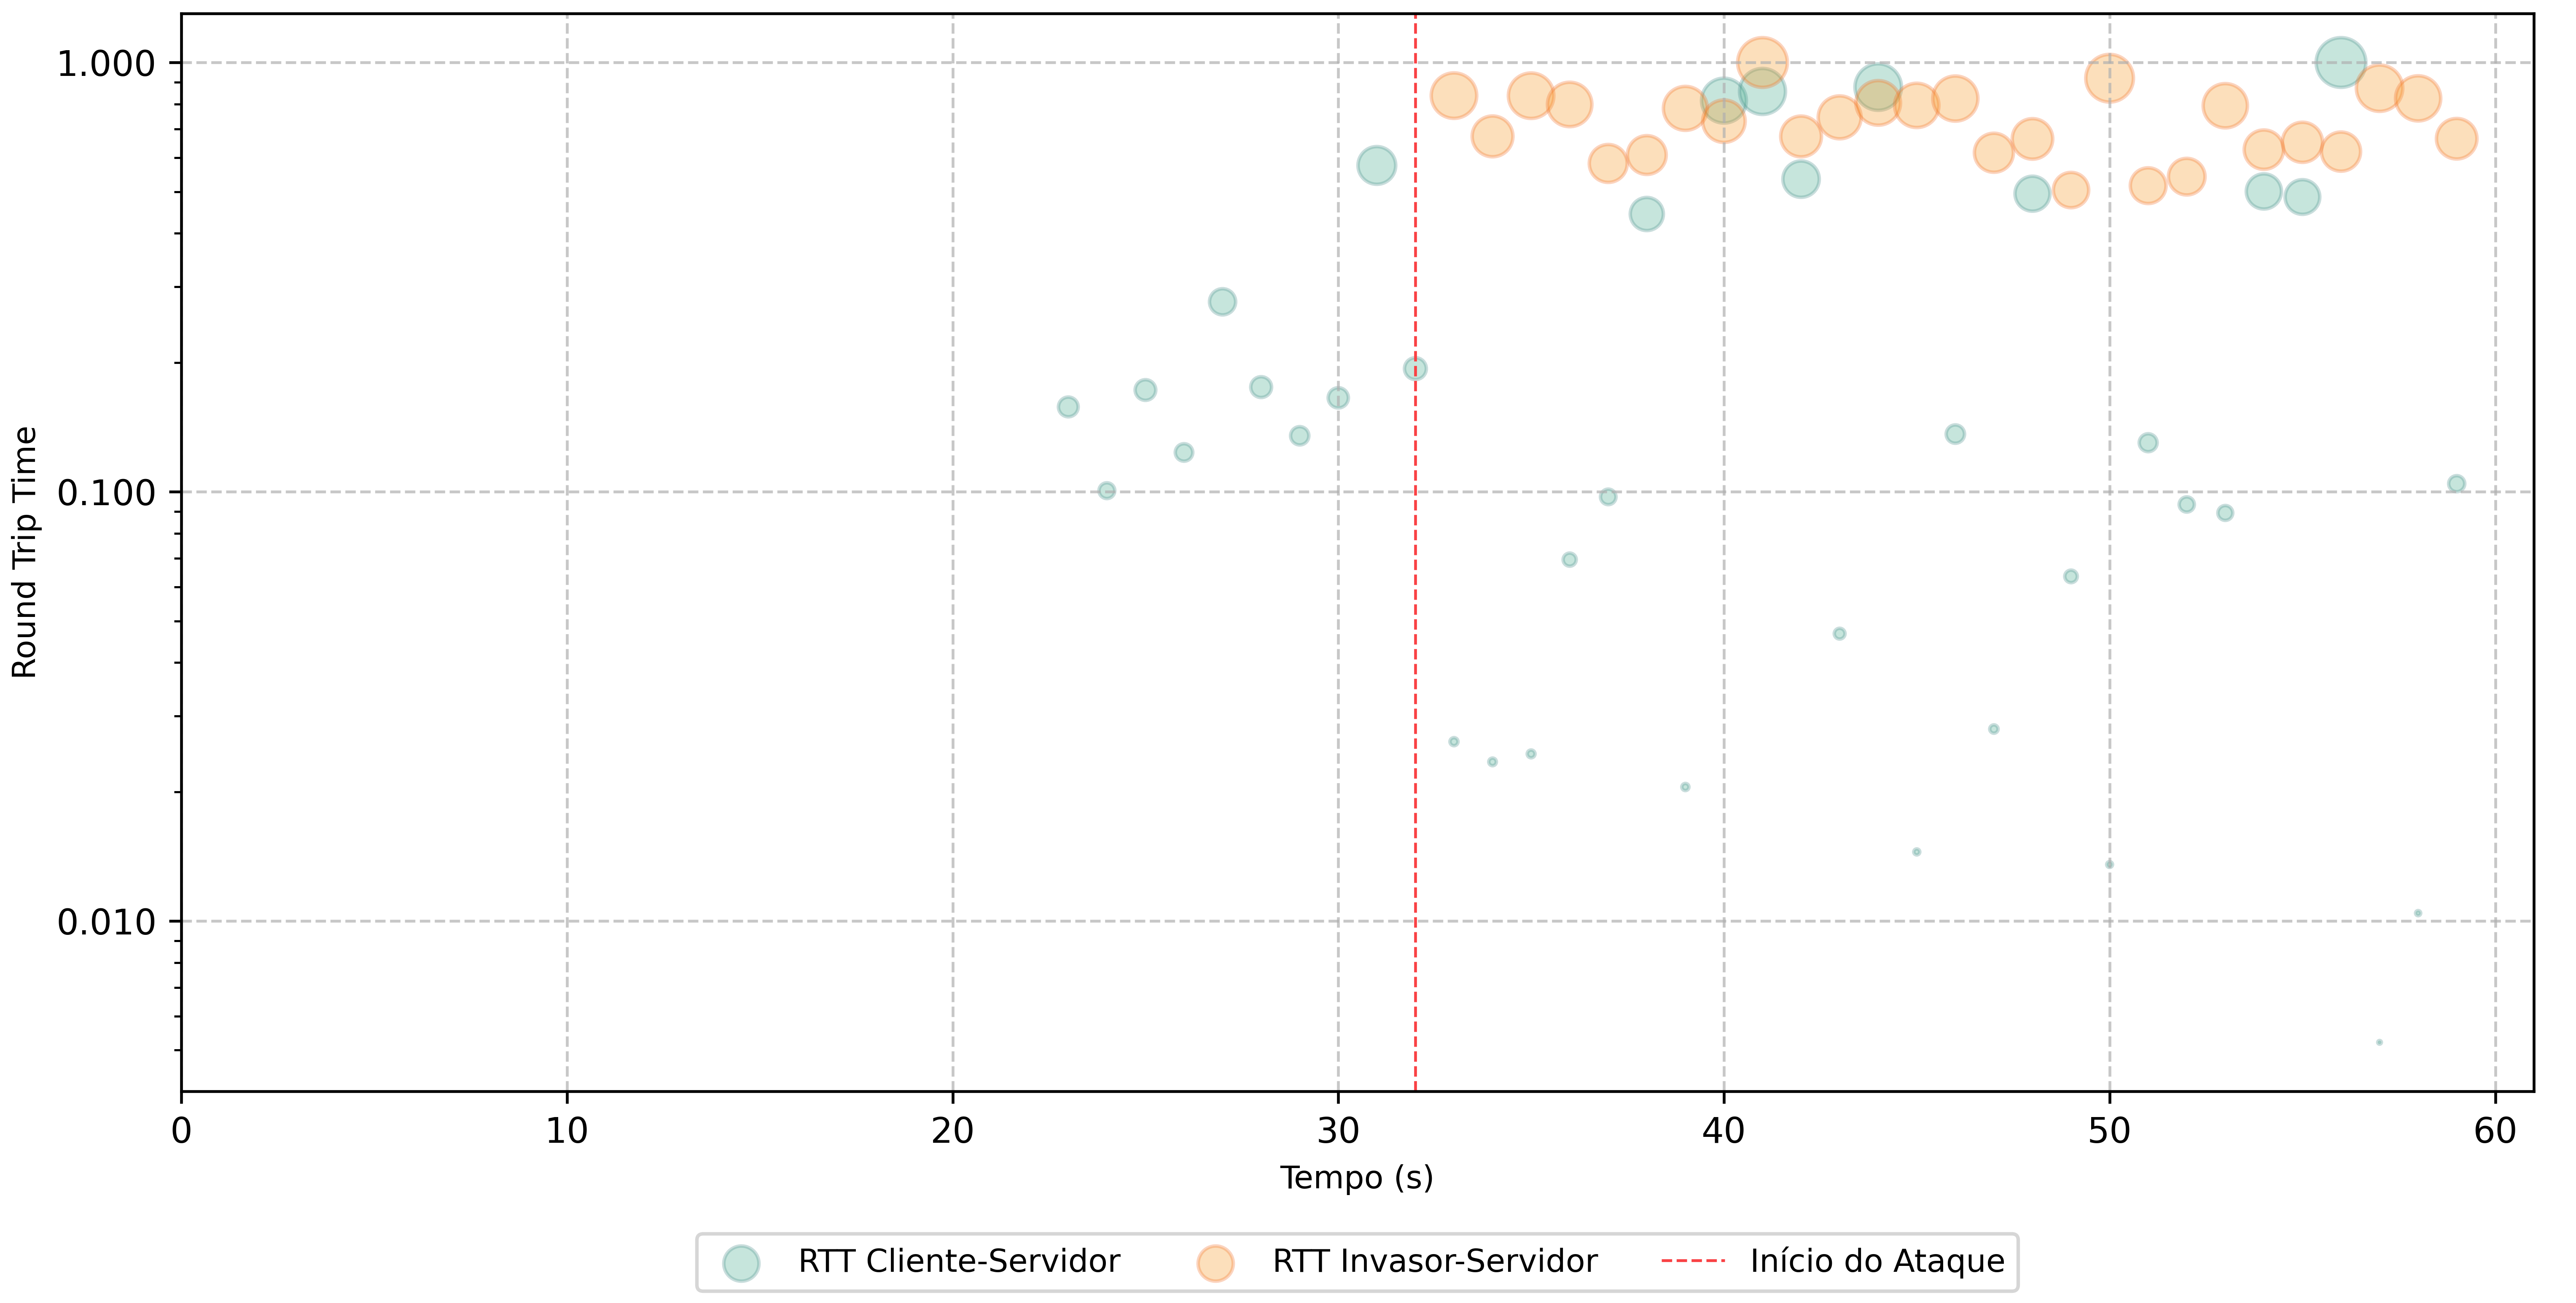
\includegraphics[width=1\textwidth, height=120pt]{USPSC-img/output/cropped/0-dos_open_multiple_secure_channels-rtts.png}
    % \end{subfigure}%
\end{figure}

\begin{figure}[htbp!]
    \centering
    \caption{\label{fig:1-dos_open_multiple_secure_channels}Gráficos do ataque de DoS pela abertura de múltiplos canais seguros - nível de segurança: `Sign'.}
    \begin{subfigure}[t]{0.5\textwidth}
        \centering
        \caption{\textit{Throughput}}
        \includegraphics[width=1\textwidth, height=120pt]{USPSC-img/output/cropped/1-dos_open_multiple_secure_channels-tput.png}
    \end{subfigure}%
    ~ 
    \begin{subfigure}[t]{0.5\textwidth}
        \centering
        \caption{Desempenho}
        \includegraphics[width=1\textwidth, height=120pt]{USPSC-img/output/cropped/1-dos_open_multiple_secure_channels-perf.png}
    \end{subfigure}%
    \\
    \begin{subfigure}[t]{0.5\textwidth}
        \centering
        \caption{Pacotes OPC UA}
        \includegraphics[width=1\textwidth, height=120pt]{USPSC-img/output/cropped/1-dos_open_multiple_secure_channels-pack.png}
    \end{subfigure}%
    ~
    \begin{subfigure}[t]{0.5\textwidth}
        \centering
        \caption{RTT por pacote}
        \includegraphics[width=1\textwidth, height=120pt]{USPSC-img/output/cropped/1-dos_open_multiple_secure_channels-rttp.png}
    \end{subfigure}%
    % ~
    % \begin{subfigure}[t]{0.5\textwidth}
    %     \centering
    %     \caption{RTT por segundos}
    %     \includegraphics[width=1\textwidth, height=120pt]{USPSC-img/output/cropped/1-dos_open_multiple_secure_channels-rtts.png}
    % \end{subfigure}%
\end{figure}

\begin{figure}[htbp!]
    \centering
    \caption{\label{fig:2-dos_open_multiple_secure_channels}Gráficos do ataque de DoS pela abertura de múltiplos canais seguros - nível de segurança: `Sign \& Encrypt'.}
    \begin{subfigure}[t]{0.5\textwidth}
        \centering
        \caption{\textit{Throughput}}
        \includegraphics[width=1\textwidth, height=120pt]{USPSC-img/output/cropped/2-dos_open_multiple_secure_channels-tput.png}
    \end{subfigure}%
    ~ 
    \begin{subfigure}[t]{0.5\textwidth}
        \centering
        \caption{Desempenho}
        \includegraphics[width=1\textwidth, height=120pt]{USPSC-img/output/cropped/2-dos_open_multiple_secure_channels-perf.png}
    \end{subfigure}%
    \\
    \begin{subfigure}[t]{0.5\textwidth}
        \centering
        \caption{Pacotes OPC UA}
        \includegraphics[width=1\textwidth, height=120pt]{USPSC-img/output/cropped/2-dos_open_multiple_secure_channels-pack.png}
    \end{subfigure}%
    ~
    \begin{subfigure}[t]{0.5\textwidth}
        \centering
        \caption{RTT por pacote}
        \includegraphics[width=1\textwidth, height=120pt]{USPSC-img/output/cropped/2-dos_open_multiple_secure_channels-rttp.png}
    \end{subfigure}%
    % ~
    % \begin{subfigure}[t]{0.5\textwidth}
    %     \centering
    %     \caption{RTT por segundos}
    %     \includegraphics[width=1\textwidth, height=120pt]{USPSC-img/output/cropped/2-dos_open_multiple_secure_channels-rtts.png}
    % \end{subfigure}%
\end{figure}

\begin{figure}[htbp!]
    \centering
    \caption{\label{fig:0-dos_translate_browse_path_call_stack_overflow}Gráficos do ataque de DoS pela tradução do caminho de navegação - nível de segurança: `None'.}
    \begin{subfigure}[t]{0.5\textwidth}
        \centering
        \caption{\textit{Throughput}}
        \includegraphics[width=1\textwidth, height=120pt]{USPSC-img/output/cropped/0-dos_translate_browse_path_call_stack_overflow-tput.png}
    \end{subfigure}%
    ~ 
    \begin{subfigure}[t]{0.5\textwidth}
        \centering
        \caption{Desempenho}
        \includegraphics[width=1\textwidth, height=120pt]{USPSC-img/output/cropped/0-dos_translate_browse_path_call_stack_overflow-perf.png}
    \end{subfigure}%
    \\
    \begin{subfigure}[t]{0.5\textwidth}
        \centering
        \caption{Pacotes OPC UA}
        \includegraphics[width=1\textwidth, height=120pt]{USPSC-img/output/cropped/0-dos_translate_browse_path_call_stack_overflow-pack.png}
    \end{subfigure}%
    ~
    \begin{subfigure}[t]{0.5\textwidth}
        \centering
        \caption{RTT por pacote}
        \includegraphics[width=1\textwidth, height=120pt]{USPSC-img/output/cropped/0-dos_translate_browse_path_call_stack_overflow-rttp.png}
    \end{subfigure}%
    % ~
    % \begin{subfigure}[t]{0.5\textwidth}
    %     \centering
    %     \caption{RTT por segundos}
    %     \includegraphics[width=1\textwidth, height=120pt]{USPSC-img/output/cropped/0-dos_translate_browse_path_call_stack_overflow-rtts.png}
    % \end{subfigure}%
\end{figure}

\begin{figure}[htbp!]
    \centering
    \caption{\label{fig:1-dos_translate_browse_path_call_stack_overflow}Gráficos do ataque de DoS pela tradução do caminho de navegação - nível de segurança: `Sign'.}
    \begin{subfigure}[t]{0.5\textwidth}
        \centering
        \caption{\textit{Throughput}}
        \includegraphics[width=1\textwidth, height=120pt]{USPSC-img/output/cropped/1-dos_translate_browse_path_call_stack_overflow-tput.png}
    \end{subfigure}%
    ~ 
    \begin{subfigure}[t]{0.5\textwidth}
        \centering
        \caption{Desempenho}
        \includegraphics[width=1\textwidth, height=120pt]{USPSC-img/output/cropped/1-dos_translate_browse_path_call_stack_overflow-perf.png}
    \end{subfigure}%
    \\
    \begin{subfigure}[t]{0.5\textwidth}
        \centering
        \caption{Pacotes OPC UA}
        \includegraphics[width=1\textwidth, height=120pt]{USPSC-img/output/cropped/1-dos_translate_browse_path_call_stack_overflow-pack.png}
    \end{subfigure}%
    ~
    \begin{subfigure}[t]{0.5\textwidth}
        \centering
        \caption{RTT por pacote}
        \includegraphics[width=1\textwidth, height=120pt]{USPSC-img/output/cropped/1-dos_translate_browse_path_call_stack_overflow-rttp.png}
    \end{subfigure}%
    % ~
    % \begin{subfigure}[t]{0.5\textwidth}
    %     \centering
    %     \caption{RTT por segundos}
    %     \includegraphics[width=1\textwidth, height=120pt]{USPSC-img/output/cropped/1-dos_translate_browse_path_call_stack_overflow-rtts.png}
    % \end{subfigure}%
\end{figure}

\begin{figure}[htbp!]
    \centering
    \caption{\label{fig:2-dos_translate_browse_path_call_stack_overflow}Gráficos do ataque de DoS pela tradução do caminho de navegação - nível de segurança: `Sign \& Encrypt'.}
    \begin{subfigure}[t]{0.5\textwidth}
        \centering
        \caption{\textit{Throughput}}
        \includegraphics[width=1\textwidth, height=120pt]{USPSC-img/output/cropped/2-dos_translate_browse_path_call_stack_overflow-tput.png}
    \end{subfigure}%
    ~ 
    \begin{subfigure}[t]{0.5\textwidth}
        \centering
        \caption{Desempenho}
        \includegraphics[width=1\textwidth, height=120pt]{USPSC-img/output/cropped/2-dos_translate_browse_path_call_stack_overflow-perf.png}
    \end{subfigure}%
    \\
    \begin{subfigure}[t]{0.5\textwidth}
        \centering
        \caption{Pacotes OPC UA}
        \includegraphics[width=1\textwidth, height=120pt]{USPSC-img/output/cropped/2-dos_translate_browse_path_call_stack_overflow-pack.png}
    \end{subfigure}%
    ~
    \begin{subfigure}[t]{0.5\textwidth}
        \centering
        \caption{RTT por pacote}
        \includegraphics[width=1\textwidth, height=120pt]{USPSC-img/output/cropped/2-dos_translate_browse_path_call_stack_overflow-rttp.png}
    \end{subfigure}%
    % ~
    % \begin{subfigure}[t]{0.5\textwidth}
    %     \centering
    %     \caption{RTT por segundos}
    %     \includegraphics[width=1\textwidth, height=120pt]{USPSC-img/output/cropped/2-dos_translate_browse_path_call_stack_overflow-rtts.png}
    % \end{subfigure}%
\end{figure}

\begin{figure}[htbp!]
    \centering
    \caption{\label{fig:0-mitm_arp}Gráficos do ataque de MITM pela falsificação da tabela ARP - nível de segurança: `None'.}
    \begin{subfigure}[t]{0.5\textwidth}
        \centering
        \caption{\textit{Throughput}}
        \includegraphics[width=1\textwidth, height=120pt]{USPSC-img/output/cropped/0-mitm_arp-tput.png}
    \end{subfigure}%
    ~ 
    \begin{subfigure}[t]{0.5\textwidth}
        \centering
        \caption{Desempenho}
        \includegraphics[width=1\textwidth, height=120pt]{USPSC-img/output/cropped/0-mitm_arp-perf.png}
    \end{subfigure}%
    \\
    \begin{subfigure}[t]{0.5\textwidth}
        \centering
        \caption{Pacotes OPC UA}
        \includegraphics[width=1\textwidth, height=120pt]{USPSC-img/output/cropped/0-mitm_arp-pack.png}
    \end{subfigure}%
    ~
    \begin{subfigure}[t]{0.5\textwidth}
        \centering
        \caption{RTT por pacote}
        \includegraphics[width=1\textwidth, height=120pt]{USPSC-img/output/cropped/0-mitm_arp-rttp.png}
    \end{subfigure}%
    % ~
    % \begin{subfigure}[t]{0.5\textwidth}
    %     \centering
    %     \caption{RTT por segundos}
    %     \includegraphics[width=1\textwidth, height=120pt]{USPSC-img/output/cropped/0-mitm_arp-rtts.png}
    % \end{subfigure}%
\end{figure}

\begin{figure}[htbp!]
    \centering
    \caption{\label{fig:1-mitm_arp}Gráficos do ataque de MITM pela falsificação da tabela ARP - nível de segurança: `Sign'.}
    \begin{subfigure}[t]{0.5\textwidth}
        \centering
        \caption{\textit{Throughput}}
        \includegraphics[width=1\textwidth, height=120pt]{USPSC-img/output/cropped/1-mitm_arp-tput.png}
    \end{subfigure}%
    ~ 
    \begin{subfigure}[t]{0.5\textwidth}
        \centering
        \caption{Desempenho}
        \includegraphics[width=1\textwidth, height=120pt]{USPSC-img/output/cropped/1-mitm_arp-perf.png}
    \end{subfigure}%
    \\
    \begin{subfigure}[t]{0.5\textwidth}
        \centering
        \caption{Pacotes OPC UA}
        \includegraphics[width=1\textwidth, height=120pt]{USPSC-img/output/cropped/1-mitm_arp-pack.png}
    \end{subfigure}%
    ~
    \begin{subfigure}[t]{0.5\textwidth}
        \centering
        \caption{RTT por pacote}
        \includegraphics[width=1\textwidth, height=120pt]{USPSC-img/output/cropped/1-mitm_arp-rttp.png}
    \end{subfigure}%
    % ~
    % \begin{subfigure}[t]{0.5\textwidth}
    %     \centering
    %     \caption{RTT por segundos}
    %     \includegraphics[width=1\textwidth, height=120pt]{USPSC-img/output/cropped/1-mitm_arp-rtts.png}
    % \end{subfigure}%
\end{figure}

\begin{figure}[htbp!]
    \centering
    \caption{\label{fig:2-mitm_arp}Gráficos do ataque de MITM pela falsificação da tabela ARP - nível de segurança: `Sign \& Encrypt'.}
    \begin{subfigure}[t]{0.5\textwidth}
        \centering
        \caption{\textit{Throughput}}
        \includegraphics[width=1\textwidth, height=120pt]{USPSC-img/output/cropped/2-mitm_arp-tput.png}
    \end{subfigure}%
    ~ 
    \begin{subfigure}[t]{0.5\textwidth}
        \centering
        \caption{Desempenho}
        \includegraphics[width=1\textwidth, height=120pt]{USPSC-img/output/cropped/2-mitm_arp-perf.png}
    \end{subfigure}%
    \\
    \begin{subfigure}[t]{0.5\textwidth}
        \centering
        \caption{Pacotes OPC UA}
        \includegraphics[width=1\textwidth, height=120pt]{USPSC-img/output/cropped/2-mitm_arp-pack.png}
    \end{subfigure}%
    ~
    \begin{subfigure}[t]{0.5\textwidth}
        \centering
        \caption{RTT por pacote}
        \includegraphics[width=1\textwidth, height=120pt]{USPSC-img/output/cropped/2-mitm_arp-rttp.png}
    \end{subfigure}%
    % ~
    % \begin{subfigure}[t]{0.5\textwidth}
    %     \centering
    %     \caption{RTT por segundos}
    %     \includegraphics[width=1\textwidth, height=120pt]{USPSC-img/output/cropped/2-mitm_arp-rtts.png}
    % \end{subfigure}%
\end{figure}

\begin{figure}[htbp!]
    \centering
    \caption{\label{fig:0-mitm_port}Gráficos do ataque de MITM pelo roubo de portas - nível de segurança: `None'.}
    \begin{subfigure}[t]{0.5\textwidth}
        \centering
        \caption{\textit{Throughput}}
        \includegraphics[width=1\textwidth, height=120pt]{USPSC-img/output/cropped/0-mitm_port-tput.png}
    \end{subfigure}%
    ~ 
    \begin{subfigure}[t]{0.5\textwidth}
        \centering
        \caption{Desempenho}
        \includegraphics[width=1\textwidth, height=120pt]{USPSC-img/output/cropped/0-mitm_port-perf.png}
    \end{subfigure}%
    \\
    \begin{subfigure}[t]{0.5\textwidth}
        \centering
        \caption{Pacotes OPC UA}
        \includegraphics[width=1\textwidth, height=120pt]{USPSC-img/output/cropped/0-mitm_port-pack.png}
    \end{subfigure}%
    ~
    \begin{subfigure}[t]{0.5\textwidth}
        \centering
        \caption{RTT por pacote}
        \includegraphics[width=1\textwidth, height=120pt]{USPSC-img/output/cropped/0-mitm_port-rttp.png}
    \end{subfigure}%
    % ~
    % \begin{subfigure}[t]{0.5\textwidth}
    %     \centering
    %     \caption{RTT por segundos}
    %     \includegraphics[width=1\textwidth, height=120pt]{USPSC-img/output/cropped/0-mitm_port-rtts.png}
    % \end{subfigure}%
\end{figure}

\begin{figure}[htbp!]
    \centering
    \caption{\label{fig:1-mitm_port}Gráficos do ataque de MITM pelo roubo de portas - nível de segurança: `Sign'.}
    \begin{subfigure}[t]{0.5\textwidth}
        \centering
        \caption{\textit{Throughput}}
        \includegraphics[width=1\textwidth, height=120pt]{USPSC-img/output/cropped/1-mitm_port-tput.png}
    \end{subfigure}%
    ~ 
    \begin{subfigure}[t]{0.5\textwidth}
        \centering
        \caption{Desempenho}
        \includegraphics[width=1\textwidth, height=120pt]{USPSC-img/output/cropped/1-mitm_port-perf.png}
    \end{subfigure}%
    \\
    \begin{subfigure}[t]{0.5\textwidth}
        \centering
        \caption{Pacotes OPC UA}
        \includegraphics[width=1\textwidth, height=120pt]{USPSC-img/output/cropped/1-mitm_port-pack.png}
    \end{subfigure}%
    ~
    \begin{subfigure}[t]{0.5\textwidth}
        \centering
        \caption{RTT por pacote}
        \includegraphics[width=1\textwidth, height=120pt]{USPSC-img/output/cropped/1-mitm_port-rttp.png}
    \end{subfigure}%
    % ~
    % \begin{subfigure}[t]{0.5\textwidth}
    %     \centering
    %     \caption{RTT por segundos}
    %     \includegraphics[width=1\textwidth, height=120pt]{USPSC-img/output/cropped/1-mitm_port-rtts.png}
    % \end{subfigure}%
\end{figure}

\begin{figure}[htbp!]
    \centering
    \caption{\label{fig:2-mitm_port}Gráficos do ataque de MITM pelo roubo de portas - nível de segurança: `Sign \& Encrypt'.}
    \begin{subfigure}[t]{0.5\textwidth}
        \centering
        \caption{\textit{Throughput}}
        \includegraphics[width=1\textwidth, height=120pt]{USPSC-img/output/cropped/2-mitm_port-tput.png}
    \end{subfigure}%
    ~ 
    \begin{subfigure}[t]{0.5\textwidth}
        \centering
        \caption{Desempenho}
        \includegraphics[width=1\textwidth, height=120pt]{USPSC-img/output/cropped/2-mitm_port-perf.png}
    \end{subfigure}%
    \\
    \begin{subfigure}[t]{0.5\textwidth}
        \centering
        \caption{Pacotes OPC UA}
        \includegraphics[width=1\textwidth, height=120pt]{USPSC-img/output/cropped/2-mitm_port-pack.png}
    \end{subfigure}%
    ~
    \begin{subfigure}[t]{0.5\textwidth}
        \centering
        \caption{RTT por pacote}
        \includegraphics[width=1\textwidth, height=120pt]{USPSC-img/output/cropped/2-mitm_port-rttp.png}
    \end{subfigure}%
    % ~
    % \begin{subfigure}[t]{0.5\textwidth}
    %     \centering
    %     \caption{RTT por segundos}
    %     \includegraphics[width=1\textwidth, height=120pt]{USPSC-img/output/cropped/2-mitm_port-rtts.png}
    % \end{subfigure}%
\end{figure}

\end{apendicesenv}
% ---